\documentclass[a4paper,oneside, 12pt]{amsart}

\usepackage[draft,
type = paper,
externalise,
figureFolder = tikzfigures,
font = libertine,
sidenotes,
math = euler,
pkgOptions={
  hyperref = {linkcolor=red},
  geometry = {a4paper, margin=3cm}
}
]{style}

\usepackage{tcolorbox}
\usetikzlibrary{quantikz2}

\addbibresource{local-bib.bib}
\usetikzlibrary{babel} % TODO: WIESO?!?
\pdfoutput=1
\title{Quantum Computing}
\author{Sebastian Halbig}
\author{Istvan Heckenberger}

%%% Some useful regexps:
% Word repetition: \(\<\w+\>\W-*\)\1

%%% --- Course specific definitions and macros

\newcommand*{\Pclass}{\ensuremath{\mathsf{P}}}
\newcommand*{\NPclass}{\ensuremath{\mathsf{NP}}}
\newcommand*{\BQPclass}{\ensuremath{\mathsf{BQP}}}
\newcommand*{\BPPclass}{\ensuremath{\mathsf{BPP}}}
\newcommand*{\Dtime}{\ensuremath{\mathbf{DTIME}}}
\DeclareMathOperator{\SWAP}{SWAP}
\DeclareMathOperator{\CNOT}{CNOT}
\newcommand*{\PauliGroup}{\ensuremath{\mathcal{P}}}


\newcommand{\underConstruction}{%
  \tikzexternaldisable
  \par\addvspace{1.5em} % Ensure new line and add space above
  \noindent
  \begingroup
  \setlength{\fboxrule}{2pt} % Thicker frame
  \setlength{\fboxsep}{10pt} % Space between frame and content
  \fbox{%
    \begin{minipage}{\linewidth-2\fboxsep-2\fboxrule}
      % Left side: The Icon
      \begin{minipage}{0.15\linewidth}
        \centering
        \scalebox{0.4}{ % Increased scale slightly for the thicker box
          
\begin{tikzpicture}[limb/.style={line cap=round,line width=1.5mm,line join=bevel}]
            \draw[line width=2mm,rounded corners,fill=yellow] (-2,0) -- (0,-2) -- (2,0) -- (0,2) -- cycle;
            \fill (1.5mm,7mm) circle (1.5mm);
            \fill(0,-7.5mm) -- ++(10mm,0mm) -- ++(120:2mm)--++(100:1mm)--++(150:2mm) arc (70:170:2.5mm and 1mm);
            \draw[limb] (-7.5mm,-6.5mm)--++(70:4mm)--++(85:4mm) coordinate(a)--++(-45:5mm)--(-2.5mm,-6.5mm);
            \fill[rotate around={45:(a)}] ([shift={(-0.5mm,0.55mm)}]a) --++(0mm,-3mm)--++
            (7mm,-0.5mm)coordinate(b)--++(0mm,4mm)coordinate(c)--cycle;
            \draw[limb] ([shift={(-0.6mm,-0.4mm)}]b) --++(-120:5mm) ([shift={(-0.5mm,-0.5mm)}]c) --++
            (-3mm,0mm)--++(-100:3mm)coordinate (d);
            \draw[ultra thick] (d) -- ++(-45:1.25cm);
          \end{tikzpicture}
        }
      \end{minipage}%
      \hfill
      % Right side: The Text
      \begin{minipage}{0.80\linewidth}
        \raggedright
        \small \textbf{Under Construction:}\\
        This part of the lecture notes is still under construction and may change over the course of the semester.
      \end{minipage}
    \end{minipage}%
  }
  \endgroup
  \par\addvspace{1.5em} % Add space below
  \tikzexternalenable
}

\begin{document}
\maketitle
\tableofcontents

\cleardoublepage

\section*{About the course}
This course is an introduction to the foundations of quantum computing, specifically designed for students in computer science, data science, mathematics, and physics.
Its goal is to provide a comprehensive overview of many important aspects of theoretical quantum computing from a mathematical perspective.
Due to the complexity of the topic, however, we will not be able to cover all aspects of (theoretical) quantum computing in a single semester.

These notes are designed to be a  self-contained and detailed companion to the lectures.
At certain points, they expand beyond the topics discussed there and provide additional background information.

\subsection*{Prerequisites}
We assume a working knowledge of vector-based linear algebra.
This includes amongst other aspects in particular the ability to compute matrix-vector and matrix-matrix products, solve (small) linear equations, and to calculate the determinant of (small) matrices.
Other mathematical topics like calculus or abstract algebra can be useful at times, though they are not required.

\subsection*{Get in touch}
We strongly encourage active in-person participation in lectures and our dedicated office hours.
In case you have questions regarding the material or the exercises, please do not hesitate to reach out via email:
\begin{itemize}
  \item \textsc{Sebastian Halbig:} \url{Sebastian.Halbig@uni-marburg.de}
  \item \textsc{Istvan Heckenberger:} \url{heckenberger@mathematik.uni-marburg.de}
\end{itemize}

\subsection*{Main resources}\label{sec:main-resources}
The course is designed around the following key resources:

\begin{itemize}[leftmargin=*]
  \item  R.\ Wolf ``Quantum Computing: Lecture Notes'' (2023), \cite{wolf2023:QuantumComputing}
  \item A.\ Kockum \etal ``Lecture Notes on Quantum Computing'' (2025), \cite{kockum-soro-garcía-álvarez-et-al2025:Lecture}
  \item A.\ Kissinger, J.\ van de Wetering, ``Picturing Quantum Software'' (2026), \cite{kissinger-wetering2025:PicturingQuantumSoftware}
  \item B.\ Coecke, A.\ Kissinger ``Picturing Quantum Processes'' (2017), \cite{coecke-kissinger2017:PicturingQuantumProcesses}
  \item M.\ Nielsen, I.\ Chuang ``Quantum Computation and Quantum Information'' (2000), \cite{nielsen-chuang2000:QuantumComputationInformation}
  % \item \cite{simon2021:TopologicalQuantum}
  % \item \cite{preskill:QuantumComputing}
\end{itemize}


\numberwithin{theorem}{section}
\cleardoublepage

\section{Why quantum computing?}\label{sec:why-quantum-computing}

To motivate why quantum computers are such a fascinating topic, we will showcase---without going into technical details---how the fundamental principles of quantum mechanics can be used to solve certain problems much faster than classical computers.
This ``quantum advantage'' relies on a rather simple shift of perspective: instead of using bit logic---expressed as maps \(f\from \{0,1\}^{n}\to\{0,1\}^{m}\)---we have (almost) the full power of linear algebra at our disposal.

\addtocontents{toc}{\SkipTocEntry}
\subsection*{The Deutsch--Jozsa algorithm}\label{sec:the-deutsch--josza-algorithm}


Consider the following problem.
For a fixed number \(n \in \mathbb{N}\), we are given a map \(f \from \{0,1\}^{n}\to\{0,1\}\).
We have no information about this map except: either it is constant or balanced.
\begin{itemize}
  \item \emph{Constant:} The output is always the same (all 0s or all 1s).
  \item \emph{Balanced:} For exactly half the possible inputs, the output is \(0\) and for the other half \(1\).
\end{itemize}
We are now given the task:
\medskip

\begin{center}
  \textit{Determine which type of function we have.}
\end{center}
\medskip

\noindent
The catch: if \(f\) is balanced, we do not know which inputs belong to the half producing 0s and which inputs result in 1s.
Thus, in the worst case, a classical computer must compute the value of \(f\) for \(2^{n-1} + 1\) inputs to conclude the type of \(f\).

\subsubsection*{The quantum approach}
In contrast to the classical solution which grows exponentially in \(n\), a quantum computer can solve the above problem with a single call to (a quantum version of) \(f\).
\begin{enumerate}
  \item[Step 1:] We initialise the system by setting up \(n+1\) qubits---the quantum version of bits.
  The first \(n\) qubits are set to \(0\) and a single trailing \(1\) qubit at the end.
  We will use the first \(n\) qubits as our ``input'' and the last qubit will function as a control qubit that captures the output of \(f\).

  \item [Step 2:] While classical gates like AND and OR would allow us to transform our first \(n\) qubits (which are \((00\dots0)\)) to some other input of \(f\) (\eg \((0101\dots 01)\)), we want to use the ``magic'' of quantum mechanics to simultaneously capture all possible inputs of \(f\).
  To that end, we use Hadamard gates.
  These transform a \(0\)-qubit into a state that is equally likely \(0\)  and \(1\).
  Applying Hadamard gates to all of our \(n+1\) qubits results in particular in our desired superposition: a combination of all possible inputs of \(f\).
  Observe that we also used a Hadamard gate to alter the control qubit.
  In the next step this will be crucial in distinguishing between the balanced and the constant case.

  \item [Step 3:] We now apply the quantum version of \(f\) to this superposition and thereafter apply  Hadamard gates again to the first \(n\) qubits.
  While the details are subtle, we can roughly think of this as creating an interference pattern that depends on \(f\).
  \begin{description}
    \item [Constructive] In case \(f\) is constant, it treats all inputs the same.
    Because of the way we set up our control qubit, this results in the components of our superposition ``adding up''.
    \item [Destructive] In contrast, if \(f\) is balanced, it treats one half of our superposition differently than the other, resulting in ``cancellations''.
  \end{description}


  \item [Step 4:] In order to determine the type of \(f\), we now simply have to measure the first \(n\) qubits.
  Due to the interference of the previous step we get two cases:
  \begin{enumerate}
    \item If all qubits are zero, the interference was constructive and \(f\) must have been constant.
    \item In case we observe anything else (at least one qubit being \(1\)), the function \(f\) must be balanced.
  \end{enumerate}
\end{enumerate}
Quite counterintuitively, the Deutsch--Jozsa algorithm is linear in the number of inputs \(n\) of \(f\).
For a classical computer, even a relatively small \(n=300\) would require more operations than there are atoms in the known universe\footnote{
  The number of atoms in the observable universe is estimated to be around \(10^{80}\). % TODO Some source
}, whereas a quantum computer could determine the type of \(f\) in merely \(603\) steps (601  Hadamard gates, 1 application of \(f\), and 1 measurement).

It is precisely this potential for exponential speedups that explains the excitement around quantum computing.



\subsection{The plan for this semester}\label{sec:the-plan-for-this-semester}

\( \)\underConstruction

The preceding exposition of the Deutsch--Jozsa algorithm raises several questions that will guide us through the semester.
\bigskip

\begin{center}
  \textit{The mathematics of quantum computing}
\end{center}
\bigskip

While we tried to convey the main ideas behind an exemplary quantum algorithm, many terms (superposition, interference, \etc) remained rather opaque.
In order to properly describe and precisely analyse quantum algorithms, we must develop a rigorous mathematical framework.
For us, this framework will be that of finite-dimensional Hilbert spaces, unitary transformations,  and orthogonal projections.

\begin{thmlist}
  \item In order to describe qubits, we will explain the \emph{SCUM rules} of~\cite{kissinger-wetering2025:PicturingQuantumSoftware}:
  \begin{enumerate}
    \item [S] \emph{States} of a quantum system correspond to vectors in a Hilbert space.
    \item [C] \emph{Compound} systems are represented by tensor products.
    \item [U] \emph{Unitary} maps realise gates.
    \item [M] \emph{Measurements} are computed according to the Born rule.
  \end{enumerate}
  \item Often, explicit matrix computations can become quite cumbersome.
  As an alternative, we will discuss the \emph{ZX-calculus}---a graphical computation method that provides a lucid description of linear maps between highly compound systems.
\end{thmlist}
\bigskip

\begin{center}
  \textit{Algorithms and applications}
\end{center}
\bigskip

As demonstrated in our exposition of the Deutsch-Jozsa algorithm, the power of quantum algorithms stems from a fundamentally different approach to computation and often requires deep insights into the problem’s structure.
To further sharpen our intuition and understanding of how the paradigm of quantum computing allows for considerable speedups compared to classical computing, we now turn to what one might call the ``big four'' quantum algorithms.

\begin{thmlist}
  \item \textbf{Deutsch--Jozsa and Simon's Algorithm:} Both address pattern recognition in functions using similar methods.
  Deutsch--Jozsa determines whether a function is balanced or constant,
  while Simon's problem asks to identify a hidden periodicity.

  \item \textbf{Shor's Algorithm:} It provides an exponential speedup for factorising integers by utilising the  the quantum Fourier transform.

  \item \textbf{Grover's Algorithm:} A probabilistic algorithm that enables efficient searching of unstructured databases, achieving a quadratic speedup over classical methods.

  \item \textbf{Harrow--Hassidim--Lloyd Algorithm:}
  Offers an efficient method for gaining insights into solutions of linear systems of equations, with the solution being encoded in the quantum state amplitudes.
\end{thmlist}
\bigskip

\begin{center}
  \textit{Quantum complexity theory}
\end{center}
\bigskip

The previous algorithms suggest an advantage of quantum computers over classical machines.
We will formalise this as a conjecture phrased in the language of complexity theory and discuss the following topics:
\noindent
\begin{thmlist}
  \item \textbf{Efficient Classical Simulation:}  The \emph{Gottesman--Knill theorem} shows that certain ``incomplete'' (in particular allowing only so-called Clifford gates) quantum computers can be efficiently simulated by a classical computer.
  \item \textbf{Universal Quantum computing:} In the classical world, a set of gates is universal if any algorithm (thought of as a map \(f\from \{0,1\}^{n}\to \{0,1\}^{m}\)) can be realised by applying these gates finitely many times.
  In stark contrast, the ``algorithms'' for a quantum computer do not form a finite set but the topological space \(\SU(2^{n})\)  (\ie a set with a notion of points being close to each other).
  A finite set of quantum gates is universal if finitely many gate applications can approximate any element of \(\SU(2^{n})\) with arbitrary precision.
  \item \textbf{The Solvay--Kitaev theorem:} Addresses the question of whether some universal gate sets are inherently more efficient than others.
  The theorem demonstrates under mild assumptions that, up to logarithmic overhead, all universal gate sets are equivalent.
  \item \textbf{An overview of complexity classes:} The class \(\Pclass\) consists of problems that are efficiently solvable by a classical computer.
  The quantum analogue is the class \(\BQPclass\) (bounded-error quantum polynomial time).
  We will formally define these classes and discuss the conjecture \(\Pclass \subsetneq \BQPclass\).
\end{thmlist}
\bigskip

\begin{center}
  \textit{Quantum error-correction}
\end{center}
\bigskip

So far, we have studied quantum computing in an idealised setting.
However, just like classical computers, we need error-correction to pass from physical to logical qubits.
Achieving fault-tolerant quantum computing is one of the most pressing challenges in the development of real-world quantum computers.

\begin{itemize}

  \item \textbf{No-Cloning Theorem:}
  Classical error correction often relies on duplicating information.
  The no-cloning theorem shows that this approach is not possible in the quantum world, necessitating alternative methods to achieving fault-tolerance.

  \item \textbf{Threshold Theorem:}
  The threshold theorem asserts that if the error rate per quantum gate is below a certain threshold, arbitrarily long quantum computations can be performed with arbitrarily small error, provided sufficient error correction is applied.
  As a consequence, universal fault-tolerant quantum computing is at least theoretically possible.

  \item \textbf{Shor’s 9-Qubit Code:}
  One of the first error-correcting codes,  demonstrating that quantum information can be protected against bit-flip and phase-flip errors.

  \item \textbf{The toric code:}
  A  system with two logical qubits, realised by combining geometric properties of the torus (\ie a doughnut) with group symmetries.
  The relevant information is encoded in global properties of these systems protecting them against all local perturbations.
\end{itemize}

\part{The mathematics of quantum computing}

\section{Linear algebra for quantum computing}\label{sec:linear-algebra-for-quantum-computing}
In the following we recapitulate basics of linear algebra necessary to discuss the axioms of quantum computing.
For further reading, see for example \cite{axler2024:LinearAlgebraDoneRight, treil2024:LinearAlgebraDoneWrong, blyth1990:ModuleTheoryLinearAlgebra}.

\subsection{Complex numbers and the binary system}\label{sec:complex-numbers}
There are two arithmetic systems at the heart of (quantum) computing: the binary system and the complex numbers.

\begin{definition}\label{def:the-field-f2}
  The binary numbers \(\mathbb{F}_{2}\) are the set \(\{0,1\}\) endowed with the maps
  \begin{align*}
    \boxplus & \from \mathbb{F}_{2} \times \mathbb{F}_{2} \to \mathbb{F}_{2}, \\
    \boxdot & \from \mathbb{F}_{2} \times \mathbb{F}_{2} \to \mathbb{F}_{2},
  \end{align*}
  called \emph{binary addition} and \emph{multiplication}, respectively.
  They are defined by the operation tables
  \begin{equation}
    \begin{array}{c|cc}
      \boxplus & 0 & 1 \\
      \hline
      0 & 0 & 1 \\
      1 & 1 & 0
    \end{array}
    \qquad\qquad
    \begin{array}{c|cc}
      \boxdot & 0 & 1 \\
      \hline
      0 & 0 & 0 \\
      1 & 0 & 1
    \end{array}.
  \end{equation}
\end{definition}

Complex numbers on the other hand subsume the real numbers and extend them by adding an imaginary part.

\begin{definition}\label{def:complex-numbers}
  The \emph{complex numbers} \( \mathbb{C} \) are the set \( \mathbb{R}^2 = \{(x, y) \mid x, y \in \mathbb{R}\} \), whose elements we write as \(x+iy\eqdef (x,y)\), endowed with two binary maps,
  \begin{align*}
    + & \from \mathbb{C} \times \mathbb{C} \to \mathbb{C}, \qquad & (a+ ib) + (x + iy) &= a+x + i(b+y), \\
    \cdot & \from \mathbb{C} \times \mathbb{C} \to \mathbb{C}, \qquad &   (a+ ib) \cdot (x +iy) &= ax - by +i(ay + bx),
  \end{align*}
  called \emph{(complex) addition} and \emph{multiplication}.
\end{definition}

Note that, while not defined as additional operations, we can \emph{subtract} complex numbers and \emph{divide} complex numbers, provided we are given a non-zero denominator.
In examples,
given \(a+ib, c+id, x+iy \in \mathbb{C}\) with \(x+iy \neq 0\), we compute
\begin{align*}
  (a+ib) - (c+id)
  & = a-c + i(b-d), \\
  \frac{1}{x+iy}
  & = \frac{x - iy}{x - iy} \frac{1}{x + iy}
    = \frac{x - iy}{x^{2} - (iy)^{2}}
    = \frac{x - iy}{x^{2}+y^{2}}.
\end{align*}

The arithmetic properties of  \( \mathbb{F}_{2}\) as well as the complex numbers \( \mathbb{C} \) are  succinctly described by stating that \( \mathbb{F}_{2}\) and \( \mathbb{C}\) form a \emph{field}.
That is, their addition and multiplication satisfy the following axioms for all elements \( a, b, c \):
\begin{thmlist}
  \item \emph{Associativity}: \((a + b) + c = a + (b + c)\) and \((a \cdot b) \cdot c = a \cdot (b \cdot c)\);
  \item \emph{Commutativity}: \( a + b = b + a \) and \( a \cdot b = b \cdot a \);
  \item \emph{Neutral elements}: \( a + 0 = a = 0 + a \) and \( a \cdot 1 = a = 1 \cdot a \);
  \item \emph{Inverses}: There exists an element \( -a \) such that \( a + (-a) = 0 \), and if \(a\neq 0\) there is an \( a^{-1}\) such that \( a \cdot a^{-1} = 1 \);
  \item \emph{Distributive law}: \( a \cdot (b + c) = a \cdot b + a \cdot c \).
\end{thmlist}

Beyond these basic algebraic properties, complex numbers have additional structure that will be essential throughout the course.

\begin{definition}\label{def:some-props-of-complex-numbers}
  Consider a complex number \( z = x + iy \in \mathbb{C} \).
  \begin{thmlist}
    \item Its \emph{real part} is \(\Re(z) = x\).
    \item Its \emph{imaginary part} is \(\Im(z) = y\).
    \item Its \emph{complex conjugate} is \(\overline{z}\eqdef x-iy\).
    \item Its \emph{absolute value} is \(|z| \eqdef \sqrt{z\overline{z}} = \sqrt{x^{2}+y^{2}}\).
  \end{thmlist}

  The \emph{unit circle} \(U(1)\eqdef\{z \in \mathbb{C} \mid |z| = 1\}\) consists of all complex numbers with absolute value \(1\).
\end{definition}

\begin{notation}
  For a complex number \(z \in \mathbb{C}\) with \(\Im(z) = 0\), we use the shorthand notation \(z \geq 0\) or \(z\leq 0\) instead of \(\Re(z) \geq 0\) and \(\Re(z) \leq 0\), respectively.
\end{notation}


We will often use the fact that any non-zero complex number can be written as a combination of its absolute value and some angle.

\begin{lemma}\label{lem:polar-form-uniqueness}
  Consider a non-zero complex number \(z= x +iy \in \mathbb{C}\).
  \begin{thmlist}
    \item There exist \((r, \alpha) \in \mathbb{R}^{2}\) with \(r>0\) such that
    \(z = re^{2\pi i \alpha}\).
    \item For any other pair \((s, \beta)\in \mathbb{R}^{2}\) satsifying \(s>0\), we have \(re^{2\pi i \alpha} = s e^{2 \pi i \beta}\) if and only if \(r=s\) and \(\alpha-\beta \in \mathbb{Z}\).
    \item We have \(x = r\cos(2 \pi \alpha)\) and \(y = r\sin(2 \pi \alpha)\), implying that \(|z| = r\).
  \end{thmlist}
\end{lemma}

\begin{equation*}
  \inputtikz{complex-numbers}
\end{equation*}

\begin{definition}\label{def:polar-decomposition}
  Consider a non-zero complex number \(z=re^{2\pi i \alpha} \in \mathbb{C}\) with \(r>0\) and \(\alpha\in \mathbb{R}\).
  We refer to \(r e^{2\pi i \alpha}\) as its \emph{polar form}, and call \(r\) the \emph{radius} and \(\alpha\) the \emph{angle} of \(z\), respectively.
\end{definition}

While it is hard to add complex numbers in polar form, it has the unquestionable advantage of simplifying complex  multiplication and division.

\begin{lemma}\label{lem:multiplication-in-polar-form}
  Let \( c = r e^{2\pi i \alpha} \) and \( d = s e^{2\pi i \beta} \) be two non-zero complex numbers in polar form.
  Their product is
  \begin{equation}
    cd = rs \; e^{2\pi i (\alpha + \beta)}.
  \end{equation}
\end{lemma}

\subsection{Vector spaces}\label{sec:vector-spaces}
The building blocks for quantum computers---qubits---will often be modelled as equivalence classes of vectors in a complex vector space.
To also succinctly cover aspects of classical computation, we use the following notation.

\begin{convention}
  For the remainder of the section, we write \(\Bbbk\in\{ \mathbb{F}_{2}, \mathbb{C}\}\).
  To maintain a unified notation, in case \( \Bbbk= \mathbb{F}_{2}\), we will often slightly deviate Definition~\ref{def:the-field-f2} and  use \(+\) instead of \(\boxplus\) and \(\cdot\) instead of \(\boxdot\).
  Additionally,we will often use juxtaposition for  multiplication.
\end{convention}

\begin{definition}\label{def:complex-vector-space}
  A \(\Bbbk\)-\emph{vector space} is a set \( V \) endowed with two maps.
  A \emph{(vector) addition} \( +\from V \times V \to V \) and a \emph{scalar multiplication} \( \cdot\from \Bbbk \times V \to V \) satisfying the following axioms for all \( s, v, w \in V \) and \( \alpha, \beta \in \Bbbk \):

  \begin{thmlist}
    \item \emph{Associativity of addition}: \( (s + v) + w = s + (v + w) \);
    \item \emph{Commutativity of  addition}: \( s + v = v + s \);
    \item \emph{Additive identity}: There exists a vector \( 0 \in V \), called the \emph{zero vector},  such that \( v + 0 = v = 0 + v \);
    \item \emph{Additive inverses}: Each vector \( v \in V \) admits an additive inverse \(-v \in V\). That is \( v + (-v) = 0 = (-v) + v \);
    \item \emph{Associativity of scalar multiplication}: \( \alpha \cdot (\beta \cdot v) = (\alpha \beta) \cdot v \);
    \item \emph{Unitality}: \( 1 \cdot v = v \).
    \item \emph{Distributivity}: \( (\alpha + \beta) \cdot (s + v) = \alpha \cdot s + \beta \cdot s + \alpha \cdot v + \beta \cdot v\).
  \end{thmlist}
  The elements of \(V\) are referred to as \emph{vectors}.

  In case \(  \Bbbk= \mathbb{C}\), we call \(V\) a \emph{complex} vector space and in case \(  \Bbbk= \mathbb{F}_{2}\), we refer to it as a \( \mathbb{F}_{2}\)-vector space.
\end{definition}

A direct computation shows that the zero vector \( 0 \in V \) and additive inverses are unique.
Furthermore, the existence of additive inverses can be derived from  the distributivity between scalar multiplication and vector addition.
For any \(v\in V\) we have
\begin{equation*}
  v + (-1)\cdot v = 1\cdot v + (-1) \cdot v = (1 -1) \cdot v = 0,
\end{equation*}
implying that \(-v = (-1)\cdot v\).

\begin{example}\label{ex:one-dim-vector-space}
  The set \( \mathbb{C} \) becomes a complex vector space with its usual complex addition and multiplication as vector addition and scalar multiplication, respectively.
  The zero vector is \( 0 \in \mathbb{C} \).

  Similarly, \( \mathbb{F}_{2}\) is an \( \mathbb{F}_{2}\)-vector space with vector addition given by \(\boxplus \from \mathbb{F}_{2} \times \mathbb{F}_{2} \to \mathbb{F}_{2}\) and scalar multiplication \(\boxdot \from \mathbb{F}_{2} \times \mathbb{F}_{2} \to \mathbb{F}_{2}\)
\end{example}

A lot of our considerations will revolve around intelligent bookkeeping for vector spaces and their transformations.
We will achieve this using a graphical calculus.
\begin{notation}\label{not:string-diagrams.}
  We will describe vector spaces, and later matrices, or linear maps using \emph{string diagrams}.
  For now these are quite simple.
  A vector space \(V\) is simply a (horizontal) line, possibly labelled by \(V\).
  The space \( \Bbbk\) will be drawn transparently.
  \begin{equation}
    \inputtikz{vector-spaces-as-string-diags}
  \end{equation}
\end{notation}

Measurements play a central role in our quantum algorithms.
These will in particular ``update'' qubits such that the resulting state is contained in a (smaller) region of  of the state space.

\begin{definition}\label{def:subspace-space}
  Consider a vector space \(V\).
  A subset \(U\subset V\) is called a \emph{subspace} of \(V\) if it is non-empty and for all \(\lambda
  \in \Bbbk \) and \(x,y \in U\) we have \(\lambda x+y \in U\).
\end{definition}

\begin{proposition}\label{prop:sub-are-vs}
  Consider a subspace \(U\) of a vector space \(V\).
  Then \(U\) becomes a vector space by restricting the vector addition and scalar multiplication of \(V\) to \(U\).
\end{proposition}

Given a vector \(v\in V\) and a subspace \(U \subset V\), we write \(v+U\eqdef\{v+u \mid u \in U\}\).

\begin{proposition}\label{prop:quotients-are-vs}
  Let \(V\) be a vector space and \(U\) a subspace.
  The set \(V/U \eqdef\{x+ U \mid x \in V\}\) becomes a vector space when endowed with the vector addition and scalar multiplication
  \begin{subequations}
    \begin{align}
      (x+U) + (y+ U) &\eqdef (x+y) +U, \label{eq:quotient-vector-addition} \\
      \lambda(x + U) &\eqdef (\lambda x) + U. \label{eq:quotient-scalar-multiplication}
    \end{align}
  \end{subequations}
\end{proposition}

\begin{definition}\label{def:quotient-vs}
  Consider a vector space \(V\) and a subspace \(U\).
  We call the vector space \(V/U\) with the vector addition and scalar multiplication of Equations~\eqref{eq:quotient-vector-addition}~and~\eqref{eq:quotient-scalar-multiplication} the \emph{quotient space} of \(V\) by \(U\).
\end{definition}

Often, we want to decompose a vector space into ``complementary'' parts.

\begin{definition}\label{def:direct-sum}
  A vector space \(V\) is said to be the \emph{(internal) direct sum} of a family of subspaces \(U_{1}, \dots , U_{n} \subset V\), called \emph{direct summands}, if for every \(v\in V\) there exist for all \(1 \leq i \leq n\) unique \(u_{i}\in U_{i}\)  such that \(u_{1}+ \dots + u_{n} = v\).

  In this case, we write \(V= U_{1} \oplus  \dots \oplus U_{n}\).
\end{definition}

Suppose \(V = U \oplus W\) is decomposed into a direct sum of two subspaces \(U\) and \(W\)
While  \(U\) and \(W\) intersect trivially, \ie \(U\cap W = \{0\}\), it is not the case that \(U \cup W = V\).
In fact, \(U \cup W\) is, in general, not even a vector space.

\begin{example}\label{ex:direct-sum-c2}
  The space \( \mathbb{C}^2=\{\begin{psmallmatrix} u \\ w \end{psmallmatrix} \mid u,w \in \mathbb{C}
  \}\) is a complex vector space with component-wise addition and scalar multiplication.
  We define the subspaces
  \(U = \{\begin{psmallmatrix} u \\ 0 \end{psmallmatrix} \mid u \in \mathbb{C}\}\) and \(W = \{\begin{psmallmatrix} 0 \\ w \end{psmallmatrix} \mid w \in \mathbb{C}\}\).
  Clearly, every vector \(v =
  \begin{psmallmatrix}
    u \\ w
  \end{psmallmatrix}
  \) of \(\mathbb{C}^{2}\) is given by the sum of two vectors \(
  \begin{psmallmatrix}
    u \\0
  \end{psmallmatrix} \in U
  \) and \(
  \begin{psmallmatrix}
    0 \\ w
  \end{psmallmatrix}
  \in W
  \).
  Therefore, \( \mathbb{C}^{2}= U \oplus W\).
\end{example}

Direct sums allude to the idea of decomposing a vector space into smaller, better manageable pieces.
Based on this idea, we want to break down a vector space into its ``simplest'' non-trivial components, leading to the notion of a basis.


\begin{definition}\label{def:basis}
  An \emph{(ordered) basis} of a \(\Bbbk\)-vector space \( V \) is a tuple \( \mathcal{B} = (b_i)_{i \in I} \), where \( I \) is a totally ordered index set, such that every vector \( v \in V \) can be written as a \emph{unique} linear combination
  \begin{equation*}
    v = \sum_{i \in I} \lambda_i b_i,
  \end{equation*}
  with \( \lambda_i \in  \Bbbk \) and only finitely many \( \lambda_i \) are non-zero.
\end{definition}

One of the most fundamental theorems in linear algebra is the existence of bases.

\begin{theorem}\label{thm:existence-of-bases-and-well-defd-dimension}
  Any vector space \(V\) admits a basis \(\mathcal{B}\).
  Moreover, any other basis \(\mathcal{A}\) of \(V\) satisfies \(|\mathcal{A}| = |\mathcal{B}|\).
\end{theorem}

While bases of a vector space are highly non-unique\footnote{Every complex vector space except \(\{0\}\) admits infinitely many bases.}, the cardinality of a basis does not, by the above result, depend on a choice.

\begin{definition}\label{def:finite-dimensional-vs}
  The \emph{dimension} of a vector space \(V\) is \(\dim V \eqdef | \mathcal{B}| \) for \(\mathcal{B}\) a basis of \(V\).

  We call \(V\) \emph{finite-dimensional} if \(\dim V < \infty\).
\end{definition}

One of the most important examples for us will be the two-dimensional complex space \( \mathbb{C}^{2}\) used to model a single qubit.

\begin{example}\label{ex:c2}
  The space \( \mathbb{C}^2=\{\begin{psmallmatrix} v \\ w \end{psmallmatrix} \mid v,w \in \mathbb{C}
  \}\) is a complex vector space with component-wise addition and scalar multiplication.
  Its \emph{standard basis} is
  \begin{equation*}
    \mathcal{E}= \big(\begin{psmallmatrix} 1 \\ 0 \end{psmallmatrix},
    \begin{psmallmatrix} 0 \\ 1 \end{psmallmatrix} \big).
  \end{equation*}
  In the context of quantum computing, one writes \(\ket{0} = \begin{psmallmatrix} 1 \\ 0 \end{psmallmatrix}\) and \(\ket{1} = \begin{psmallmatrix} 0 \\ 1 \end{psmallmatrix}\) and refers to \(\mathcal{E}\) as either the \emph{computational} or \emph{\(Z\)-basis}.
\end{example}

Similar to \( \mathbb{C}^{2}\), we can define a vector space \( \mathbb{C}^{n}\) or even \(  \Bbbk^{n}\) for any natural number \(n \in \mathbb{N}\).


\begin{example}\label{ex:cn}
  For any  natural number \(n\in \mathbb{N}\), we can define a vector space
  \begin{equation*}
    \Bbbk^n= \left\{\begin{psmallmatrix}  v_{1}\\ \vdots \\ v_{n} \end{psmallmatrix} \mid v_{1}, \dots , v_{n} \in \Bbbk \right\}
  \end{equation*}
  with pointwise addition and scalar multiplication.

  Representing elements of \( \Bbbk^{n}\) as \emph{column vectors} is not particularly space-saving.
  Thus, we will often write them as \emph{row vectors} instead.
  Explicitly, we set
  \begin{equation*}
    \begin{pmatrix}
      v_{1}\\ \vdots \\ v_{n} \end{pmatrix}^{T}
    \eqdef
    ( v_{1}, \dots, v_{n} )\qquad
    \text{for all } v=     \begin{pmatrix}
      v_{1}\\ \vdots \\ v_{n} \end{pmatrix} \in \Bbbk^{n}
  \end{equation*}
  and call \(v^{T}\) the \emph{transpose} of \(v\).


  Similar to \( \Bbbk^{2}\), it has a \emph{standard basis} \( \mathcal{E} = (e_{1}, \dots , e_{n})\) given by
  \begin{equation*}
    e_{j}^{T} \eqdef
    ( 0 , \dots , 0 , 1 , 0 , \dots , 0), \qquad \text{ with \(j\)-th entry \(1\) and all other entries \(0\).}
  \end{equation*}
\end{example}

Not all vector spaces are of the form \( \Bbbk^{n}\) for some \(n\in \mathbb{N}\).

\begin{example}\label{ex:free-vector-space}
  Let \(S\) be a set.
  We define a vector space structure on the collection \(\mathrm{Map}(S, \Bbbk)\) of all  maps \(f \from S \to \Bbbk  \) by setting
  \begin{equation*}
    (f+g)s \eqdef f(s) + g(s), \qquad (\lambda f) s \eqdef \lambda (f(s))
  \end{equation*}
  for all \(f,g \in \mathrm{Map}(S, \Bbbk)\) and \(s \in S\).

  We refer to \(\mathrm{Map}(S, \Bbbk)\) as the \emph{free \(\Bbbk\)-vector space} generated by \(S\).
  By choosing a total order on \(S\), we obtain a basis \(\mathcal{B}= (\delta_{s})_{s\in S}\) of \(\mathrm{Map}(S, \Bbbk)\), given by the \emph{delta functions}
  \begin{equation}
    \delta_{s} \from S \to \Bbbk\qquad \delta_{s}(t) =
    \begin{cases}
      1 & \text{ if } s= t, \\
      0 & \text{ otherwise},
    \end{cases} \qquad \text{ for } s\in S.
  \end{equation}

  Note that we have an inclusion
  \begin{equation*}
    \iota_{S} \from S \to \mathrm{Map}(S, \Bbbk), \qquad
    s \mapsto \delta_{s}.
  \end{equation*}

  If we identify,  by a slight abuse of notation, \(s\) with \(\iota_{S}(s) = \delta_{s}\), we can consider
  \begin{equation}
    \mathrm{Map}(S, \Bbbk) = \left\{\sum\nolimits_{s\in S} \lambda_{s} s \mid \lambda_{s}\in \Bbbk \text{ with } \lambda_{s}= 0 \text{ for all but finitely many } s\in S\right\}
  \end{equation}
  as the space of all (formal) linear combinations of \(S\).

  \textit{Mental picture for students of a computer science background:}
  We can think of the vectors in \( \mathrm{Map}(S, \Bbbk) \) as dictionaries (or associative arrays) with keys from the set \( S \) and values in \( \Bbbk \).
  For example in a Python-like pseudocode, if \( v= \texttt{ \{s: l\_s for s in S\}} \) and \(w= \texttt{ \{s: r\_s for s in S\}} \) are two vectors, then addition and scalar multiplication (by a scalar \(\lambda \in \Bbbk\))  would look like:
\begin{verbatim}
  v_plus_w = {s: v[s] + w[s] for s in S}
  lambda_v = {s: lambda * v[s] for s in S}
\end{verbatim}
\end{example}

\subsection{Matrices}\label{sec:matrices}
Matrices will play a two-fold role for us.
On the one hand, we will use them to model quantum gates.
On the other hand, they will be used to describe certain measurements.
\bigskip

For any natural number  \(n \in \mathbb{N}\), we write
\begin{equation}
  [n] \eqdef \{1, \dots , n\}.
\end{equation}
\begin{definition}\label{def:matrices}
  Consider numbers \(m, n \in \mathbb{N}\).
  An \( m \times n \) \emph{matrix} \(A\) over \( \Bbbk \) is a collection
  \begin{equation}
    A= (a_{ij})_{(i, j) \in [m] \times [n]} \eqdef
    \begin{pmatrix}
      a_{11} & a_{12} & \dots & a_{1n} \\
      a_{21} & a_{22} & \dots & a_{2n} \\
      \vdots& \ddots & & \vdots\\
      a_{m1} & a_{m2} & \dots & a_{mn}
    \end{pmatrix}
  \end{equation}
  with \(a_{ij} \in \Bbbk\) for all \(i \in [m]\) and \(j \in [n]\).
  The set of all such matrices is \( \Mat_{m,n}(\Bbbk) \).
  For \( m = n \), we write \( \Mat_n(\Bbbk) \).
\end{definition}

As we will discuss below, matrices can be used to transform vectors (via the matrix-vector multiplication).
Here, the computationally easiest case is given if all the non-zero entries of a matrix are located on the (main) diagonal.
\begin{example}\label{ex:diagonal-matrices}
  Let \(n\in \mathbb{N}\) and consider complex numbers \(\lambda_{1}, \dots , \lambda_{n} \in \Bbbk\).
  The matrix
  \begin{equation}
    \mathrm{diag}(\lambda_{1}, \dots , \lambda_{n}) =
    \begin{pmatrix}
      \lambda_1 & 0 & \cdots & 0 \\
      0 & \lambda_2 & & \vdots \\
      \vdots & & \ddots & 0 \\
      0 & \cdots & 0 & \lambda_n
    \end{pmatrix}
  \end{equation}
  is called a \emph{diagonal matrix}.
  In case \(\lambda_{1}= \dots = \lambda_{n} = 1\), we write \(I_{n}\eqdef \mathrm{diag}(1, \dots ,1)\in \Mat_{n}(\Bbbk)\) and call it the \emph{identity matrix} of size \(n\).
\end{example}

The ``power'' of quantum computing arises from the calculus of non-diagonal matrices.
The two examples below will be fundamental throughout the course.

\begin{example}\label{ex:Hadamard-and-cnot-gate}
  The  matrix
  \begin{equation*}
    \begin{pmatrix}
      \tfrac{1}{\sqrt{2}} & \tfrac{1}{\sqrt{2}} \\
      \tfrac{1}{\sqrt{2}} & -\tfrac{1}{\sqrt{2}}
    \end{pmatrix} \in \Mat_{2}( \mathbb{C})
  \end{equation*}
  is called the \emph{Hadamard gate} in quantum computing and will be used to create superpositions.

  The \emph{CNOT}-gate is given by the matrix
  \begin{equation*}
    \begin{pmatrix}
      1 & 0 & 0 & 0 \\
      0 & 1 & 0 & 0 \\
      0 & 0 & 0 & 1 \\
      0 & 0 & 1 & 0
    \end{pmatrix}\in \Mat_{4}( \mathbb{C}).
  \end{equation*}
  We will later see how it can be used to flip a \emph{target qubit} depending on the behaviour of a \emph{control qubit}.
  This will be a source of producing entanglements.
\end{example}

One of the most important set of matrices are the Pauli-matrices.
\begin{definition}\label{def:Pauli-matrices}
  The complex matrices
  \begin{equation*}
    \sigma_x =
    \begin{pmatrix}
      0& 1 \\ 1& 0
    \end{pmatrix}, \qquad
    \sigma_{y} =
    \begin{pmatrix}
      0 & -i \\ i & 0
    \end{pmatrix},\qquad
    \sigma_{z} =
    \begin{pmatrix}
      1 & 0 \\ 0 & -1
    \end{pmatrix}
  \end{equation*}
  are called \emph{Pauli matrices}.
\end{definition}
For convenience, we also write \(\sigma_{0} = I_{2}\eqdef
\begin{psmallmatrix}
  1 & 0 \\ 0 & 1
\end{psmallmatrix}.
\)

\begin{remark}\label{rmk:matrices-are-a-vector-space}
  The set \( \Mat_{m,n}(\Bbbk) \) of \( m \times n \) matrices forms a complex vector space under entry-wise addition and scalar multiplication.
  Specifically, for \( \lambda \in \Bbbk \) and \( A, B \in \Mat_{m,n}(\Bbbk) \), we define
  \begin{subequations}
    \begin{gather}
      A + B =
      \begin{pmatrix}
        a_{11} & \dots &  a_{1n} \\
        \vdots & \ddots & \vdots \\
        a_{m1} & \dots &  a_{mn}
      \end{pmatrix}
      +
      \begin{pmatrix}
        b_{11} & \dots &  b_{1n} \\
        \vdots & \ddots & \vdots \\
        b_{m1} & \dots &  b_{mn}
      \end{pmatrix}
      \eqdef \begin{pmatrix}
        a_{11} + b_{11} & \dots & a_{1n} + b_{1n} \\
        \vdots & \ddots & \vdots \\
        a_{m1} + b_{m1} & \dots & a_{mn} + b_{mn}
      \end{pmatrix}, \\
      \lambda A =
      \lambda
      \begin{pmatrix}
        a_{11} & \dots &  a_{1n} \\
        \vdots & \ddots & \vdots \\
        a_{m1} & \dots &  a_{mn}
      \end{pmatrix}
      \eqdef \begin{pmatrix}
        \lambda a_{11} & \dots & \lambda a_{1n} \\
        \vdots & \ddots & \vdots \\
        \lambda a_{m1} & \dots & \lambda a_{mn}
      \end{pmatrix}.
    \end{gather}
  \end{subequations}
\end{remark}

While qubits are often described as equivalence classes of vectors in a complex vector space, there is an equivalent formulation via density matrices.
These are matrices which are, amongst other properties, invariant under the transformations discussed in the next definition.

\begin{definition}\label{def:adjoint}
  Consider a matrix \( A = (a_{ik}) \in \Mat_{m,n}(  \Bbbk) \).
  \begin{thmlist}
    \item The \emph{transpose} of \( A \) is \( A^T = (a_{ki}) \in \Mat_{n,m}(\mathbb{  \Bbbk}) \).
  \end{thmlist}
  Now, let \(  \Bbbk= \mathbb{C}\).
  \begin{thmlist}[resume]
    \item The \emph{conjugate} of \( A \) is \( \overline{A} = (\overline{a_{ik}}) \in \Mat_{m,n}(\mathbb{C}) \).
    \item The \emph{adjoint} of \( A \) is \( A^\dagger = \overline{A^T} \in \Mat_{n,m}(\mathbb{C}) \).
  \end{thmlist}
  In the case \( m = n \) and \( A = A^\dagger \), we call \( A \) \emph{self-adjoint} or \emph{Hermitian}.
\end{definition}


We want to perform two operations with our quantum gates:
we want to apply them to a state and we want to compose them (\ie, apply multiple ones in sequence).
The former operation will be modelled by matrix-vector multiplication.
The latter by matrix-matrix multiplication.

\begin{definition}\label{def:matrix-multiplication}
  Let \( A = (a_{ik}) \in \Mat_{m,n}(\Bbbk) \) be a matrix.
  \begin{thmlist}
    \item Consider a vector \(v\in \Bbbk^{n}\) with \(v^{T}= (v_{1}, \dots , v_{n})\).
    The \emph{matrix-vector multiplication} of \(A\) and \(v\) is the vector \(Av \in \Bbbk^{m}\) defined by
    \begin{equation}
      (Av)_{i} \eqdef \sum_{k=1}^{n} a_{ik} v_{k}.
    \end{equation}
    \item Given another matrix \( B = (b_{kj}) \in \Mat_{n,p}(\Bbbk) \), the \emph{matrix product} of \(A\) and \(B\) is the matrix \( AB \in \Mat_{m,p}(\Bbbk) \) whose entries are given for all \(1\leq i \leq m\) and \(1\leq j \leq p\) by
    \begin{equation*}
      (AB)_{ij} = \sum_{k=1}^n a_{ik} b_{kj}.
    \end{equation*}
  \end{thmlist}
\end{definition}

The above formula for the product of two matrices can be memorised as follows.
Consider matrices \(A\in \Mat_{m,n}(\Bbbk)\) and \(B \in \Mat_{n,p}( \Bbbk)\).
Suppose, we want to determine the entry \(C_{ij}\) of the product \(C= AB \in \Mat_{m,p} (\Bbbk)\).
To that end, we proceed in two steps.
\begin{thmlist}
  \item We consider the (row)  vector \(a= (a_{i1}\;  \dots \; a_{in})\) given by the \(i\)-th row of \(A\) and the (column) vector \(b = \begin{psmallmatrix} b_{1j}\\ \vdots \\b_{nj}  \end{psmallmatrix}
  \) given by the \(j\)-th column of \(B\).
  \item Then \( C_{ij} \) is the ``dot product'' of \( a \) and \( b \).
  That is,
  \begin{equation*}
    C_{ij}=
    \begin{pmatrix}
      a_{i1} & a_{i2} & \dots & a_{in}
    \end{pmatrix}
    \begin{pmatrix}
      b_{1j} \\
      b_{2j} \\
      \vdots \\
      b_{nj}
    \end{pmatrix}
    =
    a_{i1}b_{1j} + a_{i2} b_{2j} + \dots + a_{in}b_{nj}.
  \end{equation*}
\end{thmlist}
To see this pattern of combining columns and rows, consider the matrices
\begin{equation*}
  A = \begin{pmatrix}
    {\color{red}{\mathbf{a_{11}}}} & {\color{red}{\mathbf{a_{12}}}} \\
    {\color{dark blue}{a_{21}}} & {\color{dark blue}{a_{22}}}
  \end{pmatrix}, \quad
  B = \begin{pmatrix}
    {\color{dark green}{\mathbf{b_{11}}}} & {\color{pastel orange}{b_{12}}} \\
    {\color{dark green}{\mathbf{b_{21}}}} & {\color{pastel orange}{b_{22}}}
  \end{pmatrix}.
\end{equation*}
The product \( C = AB \) is
\begin{equation*}
  C =
  \begin{pmatrix}
    {\color{red}{\mathbf{a_{11}}}}{\color{dark green}{\mathbf{b_{11}}}} + {\color{red}{\mathbf{a_{12}}}}{\color{dark green}{\mathbf{b_{21}}}} & & {\color{red}{a_{11}}}{\color{pastel orange}{b_{12}}} + {\color{red}{a_{12}}}{\color{pastel orange}{b_{22}}} \\
    {\color{dark blue}{a_{21}}}{\color{dark green}{b_{11}}} + {\color{dark blue}{a_{22}}}{\color{dark green}{b_{21}}} & & {\color{dark blue}{a_{21}}}{\color{pastel orange}{b_{12}}} + {\color{dark blue}{a_{22}}}{\color{pastel orange}{b_{22}}}
  \end{pmatrix}.
\end{equation*}
A pure colour comparison shows that \eg the entry \(C_{11}\) of \(C\) is obtained by combining the first row of \(A\) with the first column of \(B\).

\begin{notation}\label{not:string-diags-for-matrices}
  In string diagrams, we represent matrices as labelled boxes between lines.
  To keep the diagrams lucid, we omit drawing identity matrices.
  As a convention, we read our diagrams from right to left.
  \begin{equation}
    \inputtikz{matrices-as-string-diags}
  \end{equation}
  Matrix multiplication is given by horizontally concatenating diagrams.
  \begin{equation}
    \inputtikz{matrix-matrix-mult-as-string-diags}
  \end{equation}

  We can also express taking transposes, adjoints, and conjugates in our diagrammatic formalism.
  \begin{equation}
    \inputtikz{matrix-transpose-adjoint-conjugate}
  \end{equation}

  To also express matrix-vector multiplication, we may consider a vector \(v \in \Bbbk^{n}\) as a matrix \(v\in \Mat_{n,1}( \Bbbk)\).
  To signify that \(v\) is a vector, we draw it as a triangle.
  \begin{equation}
    \inputtikz{matrix-vector-mult-as-string-diags}
  \end{equation}
\end{notation}

To ensure that the diagrammatic approach to matrix operations is well-defined, we implicitly use that matrix multiplication is associative and the identity matrix is a multiplicative identity.

\begin{lemma}\label{lem:associativity-of-matrix-multiplication}
  Matrix multiplication is associative and unital.
  That is, for all \(A \in \Mat_{m,n}( \Bbbk)\), \(B \in \Mat_{n,o}( \Bbbk)\), and \( C \in \Mat_{o,p}( \Bbbk)\), we have
  \begin{equation*}
    A(BC) = (AB)C \qquad \text{and}\qquad
    I_{m} A = A = A I_{n}.
  \end{equation*}
\end{lemma}
Note however, that matrix multiplication is \emph{not} commutative.
For every \(n\geq 2\) there are square matrices \(A, B \in \Mat_{n,n}(\Bbbk)\), such that \(AB \neq BA\).

\begin{example}\label{ex:multiplication-table}
  The multiplication table of the Pauli matrices of Definition~\ref{def:Pauli-matrices} (with \(\sigma_{0}=I_{2}\)) is as follows:
  \begin{equation*}
    \begin{array}{l| c c c c}
      & \sigma_{0} & \sigma_{x} & \sigma_{y} & \sigma_{z} \\\hline
      \sigma_{0} & \sigma_{0} & \sigma_{x} & \sigma_{y} & \sigma_{z} \\
      \sigma_{x} & \sigma_{x} & \sigma_{0} & i \sigma_{z} & i\sigma_{y} \\
      \sigma_{y} & \sigma_{y} & -i \sigma_{z} & \sigma_{0} & i\sigma_{x} \\
      \sigma_{z} & \sigma_{z} & -i \sigma_{y} & - i\sigma_{x} & \sigma_{0}
    \end{array}
  \end{equation*}
\end{example}

\begin{definition}\label{def:invertible-matrix}
  Let \(n\in \mathbb{N}\) be a natural number.
  A matrix \( A \in \Mat_n(\Bbbk) \) is \emph{invertible} if there exists a matrix \( B \in \Mat_n(\Bbbk) \) such that \( AB = I_n = BA \), where \( I_n \) is the \( n \times n \) identity matrix.
  In this case, \( B \) is called the \emph{inverse} of \( A \) and is denoted by \( A^{-1} \eqdef B\).

  The set of invertible matrices is \(\GL_{n}( \Bbbk)\).
\end{definition}
The inverse of an invertible matrix \(A\in \Mat_{n}( \Bbbk)\) can be computed for example using Gaussian elimination.
Starting with
\begin{equation*}
  \left(\begin{array}{cccc|cccc}
    a_{11}& a_{12} & \dots & a_{1n}& 1 & 0 & \dots & 0 \\
    a_{21}& \ddots & \ddots & \vdots& 0 & \ddots &\ddots & \vdots \\
    \vdots& \ddots & \ddots & a_{n-1 \;n}& \vdots & \ddots & \ddots & 0 \\
    a_{n1}& \ddots & a_{n\; n-1} & a_{nn}& 0 & \dots & 0 & 1
  \end{array}\right),
\end{equation*}
we apply elementary (row) transformations until we reach a matrix of the form
\begin{equation*}
  \left(\begin{array}{cccc|cccc}
     1 & 0 & \dots & 0 & b_{11}& b_{12} & \dots & b_{1n} \\
     0 & \ddots & \ddots & \vdots & b_{21}& \ddots & \ddots & \vdots \\
    \vdots & \ddots & \ddots & 0 & \vdots& \ddots & \ddots & b_{n-1 \;n} \\
    0 & \dots & 0 & 1 & b_{n1}& \ddots & b_{n\; n-1} & b_{nn}
  \end{array}\right).
\end{equation*}
The matrix \(B=(b_{ij})\) is the inverse of \(A\).
\bigskip

Three interconnected invariants of matrices will play a central role in the study of quantum computing: the rank, trace and the determinant of a matrix (the latter indirectly, and mostly via its connection to eigenvalues).

\begin{definition}\label{def:rank}
  The \emph{rank} \(\rk(A)\) of a matrix \(A \in \Mat_{m,n}(\Bbbk)\) is the dimension of the subspace \(\{ Av \mid v\in \Bbbk^{n}\}\subset \Bbbk^{m}\).
\end{definition}

The rank of a matrix \( A \in \Mat_{m,n}(\Bbbk) \) can be computed using Gaussian elimination.
By applying elementary row operations (swapping rows, multiplying a row by a non-zero scalar, and adding a multiple of one row to another), we can transform \( A \) into a matrix \(A'\) in  \emph{row echelon form}.
That is, a matrix of the form
\begin{equation*}
  A' = \left(
    \begin{array}{cccccccccc}
      0 & \dots & 0 &\multicolumn{1}{|c}{\mathbf{a_{1j_{1}}}} & \dots  & \dots& \dots & \dots & \dots  & a_{1n} \\
      \cline{4-5}
      0 & \dots & \dots & \dots & 0 &  \multicolumn{1}{|c}{\mathbf{a_{2j_{2}}}} & \dots & \dots & \dots & a_{2n} \\
      \cline{6-7}
      \vdots & \vdots & \vdots & \vdots & \vdots & \vdots & \vdots & \vdots & \vdots  & \vdots\\
      0 & \dots & \dots & \dots & \dots & \dots &  0 & \multicolumn{1}{|c}{\mathbf{a_{kj_{k}}}} &\dots &  a_{3n} \\
      \cline{8-10}
      0 & \dots & \dots & \dots  & \dots & \dots & \dots & \dots & \dots & 0\\
      \vdots & \vdots & \vdots & \vdots & \vdots & \vdots & \vdots & \vdots & \vdots  & \vdots\\
    \end{array}
  \right)
\end{equation*}
with \((a_{1j_{1}}, \dots , a_{kj_{k}})\)  non-zero.
These elements are called the \emph{pivot elements} of \(A'\).
The rank \(\rk (A) = k\) simply equals the number of \emph{pivot} elements of \(A'\).


\begin{definition}\label{def:trace}
  The \emph{trace} of a matrix \(A\in \Mat_{n}( \Bbbk)\) is
  \begin{equation}
    \tr(A)= a_{11}+ \dots + a_{nn}.
  \end{equation}
\end{definition}

In the density matrix formalism, traces will be used to describe probabilities of outcomes of measurements.

\begin{proposition}\label{prop:basic-properties-of-trace}
  Let \(A, B\in \Mat_{n}( \Bbbk)\), \(\lambda \in \Bbbk\), and \(G \in \GL_{n}( \Bbbk)\).
  The trace  is
  \begin{thmlist}
    \item linear:  \(\tr(\lambda A + B) = \lambda \tr(A) + \tr(B)\),
    \item cyclic: \(\tr(AB) = \tr(BA)\), and
    \item invariant under conjugation: \(\tr(GAG^{-1}) = \tr(A)\).
  \end{thmlist}
\end{proposition}

Eigenvalues play a crucial role in quantum computing, for example via their connection to positive (semi-)definiteness.

\begin{definition}\label{def:eigenvalue-and-eigenspace}
  Let \( A \in \Mat_{n}(\Bbbk) \). A scalar \( \lambda \in \Bbbk \) is called an \emph{eigenvalue} of \( A \) if there exists a non-zero vector \( v \in \Bbbk^n \) such that
  \begin{equation}
    A v = \lambda v.
  \end{equation}

  The vector \( v \) is called an \emph{eigenvector} associated with \( \lambda \).
  The subspace \(\{v\in \Bbbk^{n} \mid Av = \lambda v\}\) is the \emph{eigenspace} of the eigenvalue \( \lambda \).
\end{definition}

For computations, it is often favourable to work with \emph{diagonal matrices}.
That is, matrices with all off-diagonal entries being zero.

\begin{definition}\label{def:diagonalisable}
  A matrix \( A \in \Mat_{n}(\Bbbk) \) is \emph{diagonalisable} if there exists an invertible matrix \( P \in \Mat_{n}(\Bbbk) \) such that
  \begin{equation*}
    P^{-1} A P =
    \begin{pmatrix}
      \lambda_1 & 0 & \dots & 0 \\
      0 & \lambda_2 & & \vdots \\
      \vdots & & \ddots & 0 \\
      0 & \cdots & 0 & \lambda_n
    \end{pmatrix}.
  \end{equation*}
  is a diagonal matrix.
\end{definition}

The connection between eigenvalues and diagonalisable matrices is due to the following result.

\begin{proposition}\label{prop:diag-iff-basis-of-eigenvalues}
  A matrix \( A \in \Mat_{n}(\Bbbk) \) is diagonalisable if and only if there exists a basis \( \mathcal{B} = (b_1, \dots, b_n) \) of \( \Bbbk^n \) consisting of eigenvectors of \( A \).

  In this case, let \( B \) be the matrix whose columns are the eigenvectors \( b_1, \dots, b_n \), and set \( \lambda_k \in \Bbbk \)  such that \(Ab_{k}=\lambda_{k}b_{k}\) for all \(1\le k \leq n\).
  Then,
  \begin{equation}
    B^{-1} A B =
    \begin{pmatrix}
      \lambda_1 & 0 & \cdots & 0 \\
      0 & \lambda_2 & & \vdots \\
      \vdots & & \ddots & 0 \\
      0 & \cdots & 0 & \lambda_n
    \end{pmatrix}.
  \end{equation}
\end{proposition}

The determinant is a fundamental tool for finding the eigenvalues of a matrix.
Specifically, eigenvalues of a matrix \(A\) correspond to roots of the so-called characteristic polynomial \(\chi_{A}(\lambda)\).

\begin{definition}\label{def:permutation}
  For a given \( n \in \mathbb{N} \), the set of all \emph{permutations} of \( \{1, \dots, n\} \) is
  \begin{equation}
    \Sym(n) \eqdef \{\sigma \from [n] \to [n] \mid \sigma \text{ is bijective}\}.
  \end{equation}
  The \emph{signum} of a permutation \( \sigma \) is
  \begin{equation}
    \sgn(\sigma) = \prod_{1\leq i<j \leq n}\frac{\sigma(j)-\sigma(i)}{j-i} \in \{\pm 1\}.
  \end{equation}
\end{definition}

The following definition of the determinant is called the \emph{ Leibniz formula}.
Equivalent definitions can be given in terms of the Laplace formula, or the universal property of the determinant as alternating and normalised multilinear form.
\begin{definition}\label{def:determinant}
  The \emph{determinant} of a matrix \( A = (a_{ij}) \in \Mat_n(\Bbbk) \) is
  \begin{equation}
    \det(A) = \sum_{\sigma \in \Sym(n)} \sgn(\sigma) a_{1\sigma(1)} \cdots a_{n\sigma(n)}.
  \end{equation}
\end{definition}

Unlike traces, the determinant is not linear\footnote{%
  It is however, linear in the columns and rows of a matrix, respectively.}.

\begin{proposition}\label{prop:basic-properties-of-determinant}
  Consider matrices \(A, B \in\Mat_{n}( \Bbbk) \) and \(P \in \GL_{n}( \Bbbk)\).
  The determinant is
  \begin{thmlist}
    \item multiplicative: \(\det(AB) = \det(A) \det (B)\),
    \item normalised: \(\det(I_{n}) = 1\), and
    \item invariant under conjugation: \(\det(PAP^{-1})= \det(A)\).
  \end{thmlist}
\end{proposition}

One shows that \(A\in \Mat_{n}( \Bbbk)\) is invertible if and only if \(\det(A) \neq 0\).
This can be cleverly used to study eigenvalues.
Suppose that \(\lambda\) is an eigenvalue of \(A\) and \(v \in \Bbbk^{n}\) is an eigenvector
Then
\begin{equation*}
  (\lambda I_{n} - A) v = \lambda I_{n} v - Av = \lambda v - \lambda v =0.
\end{equation*}
Since \(0 \neq v\) the matrix \(\lambda I_{n} - A\) cannot be invertible and \(\det (\lambda I_{n} - A) = 0\).
Thus, we want to systematically find all \(t \in \Bbbk\) such that  \(\det(t I_{n} - A) = 0\).

\begin{definition}\label{def:char-poly}
  The \emph{characteristic polynomial} of a matrix \( A \in \Mat_n(\Bbbk) \) is
  \begin{equation}
    \chi_A(t) = \det(t I_n - A) \in \Bbbk[t].
  \end{equation}
\end{definition}
We can now state our previously made observation about the connection between eigenvalues and determinants as a theorem.
\begin{theorem}\label{thm:eigenvalues-and-char-poly}
  A scalar \(\lambda \in \Bbbk\) is an eigenvalue of a matrix \(A\in \Mat_{n}( \Bbbk)\) if and only if \(\chi_{A}(\lambda) = 0\).
\end{theorem}

The coefficients of the characteristic polynomial are closely connected with the invariants of matrices we have previously discussed.

\begin{proposition}\label{prop:coeffs-of-char-poly}
  The characteristic polynomial of a matrix \(A \in \Mat_{n}( \Bbbk)\) satisfies
  \begin{equation}
    \chi_{A}(t) = t^{n} - \tr(A)t^{n-1} + \dots + (-1)^{n}\det(A).
  \end{equation}
\end{proposition}
Let \(v\in \Bbbk^{n}\) be a vector and \(A \in \Mat_{n}( \Bbbk)\) a matrix.
By considering \(v^{\dagger}= (\overline{v_{1}}, \dots , \overline{v_{n}})\in \Mat_{1,n}( \Bbbk)\) as a matrix, we can compute the scalar
\begin{equation*}
  v^{\dagger}Av =\sum_{i,k=1}^{n} \overline{v_{i}}a_{ik}v_{k} \in \Bbbk.
\end{equation*}

\begin{definition}\label{def:positive-semidefinite}
  A self-adjoint matrix \(A\in \Mat_{n}( \mathbb{C})\) is \emph{positive semidefinite} if one of the following equivalent conditions hold
  \begin{thmlist}
    \item For all \(v\in \mathbb{C}^{n}\) we have \(v^{\dagger}Av \geq 0\).
    \item All eigenvalues \(\lambda\) of \(A\) are real and \(\lambda \geq 0\).
    \item For every \(1\leq i\leq n\), every \emph{i-th principal minor} is non-negative.
    The \(i\)-th principal minors are the determinants \(\det A_{i}\) of  the \( i \times i \) submatrices of \(A\) obtained by deleting the same \( n-i \) rows \(l_{1}, \dots , l_{i}\) and columns \(l_{1}, \dots , l_{i}\) from \( A \).
  \end{thmlist}
\end{definition}
The criterion involving principal minors requires checking \emph{all} possible \( i \times i \) principal minors for each \( i \), not just the leading principal minors (those formed by the first \( i \) rows and columns).
For example, for a self-adjoint \( 2 \times 2 \) matrix
\begin{equation*}
  A = \begin{pmatrix}
    a & b \\
    \overline{b} & d
  \end{pmatrix},
\end{equation*}
the principal minors are:
\begin{thmlist}
\item \( i = 1 \): we delete the first row and first column, and get the matrix \((a)\) whose determinant is \( \det(a)=a \),
\item \( i = 1 \): we delete the second row and second column, leading to the matrix \((d)\) with  determinant \( \det(d)=d\).
\item \( i = 2 \): we consider the whole matrix and have \( \det(A) = ad - b\overline{b} \),
\end{thmlist}
Cases like deleting the first row and the second column are not considered.
\bigskip

Albeit an abstract result at first glance, the Cayley--Hamilton theorem describes many of the structural properties of matrices.
\begin{theorem}[Cayley--Hamilton]\label{thm:cayley-hamilton}
  Every matrix \( A \in \Mat_n(\Bbbk) \) satisfies
  \begin{equation*}
    \chi_{A}(A) = 0 \in \Mat_{n}( \Bbbk).
  \end{equation*}
\end{theorem}
Here, \( \chi_A(A) \) is the matrix obtained by substituting \( A^k \) for \( t^k \) in the characteristic polynomial \( \chi_A(t) \), with the convention that \( A^0 = I_n \).
For example,  the \(2 \times 2\)-matrix \(A =\begin{psmallmatrix} a & b \\ c & d \end{psmallmatrix}\)
has the characteristic polynomial
\begin{equation*}
  \chi_A(t) = \det(t I_2 - A) = t^2 - (a + d)t + (ad - bc)
\end{equation*}
and inserting \(A\) yields
\begin{equation*}
  \chi_{A}(A) = A^{2} - (a + d) A + (ad-bc) I_{2} = A^{2} - \tr(A)A + \det(A)I_{2}.
\end{equation*}

\begin{corollary}\label{cor:consequences-of-caley-hamilton}
  Consider a square matrix \( A \in \Mat_n(\mathbb{C}) \) with characteristic polynomial \(\chi_{A}(t) = t^{n} + c_{n-1} t^{n-1} + \dots + c_{1}t + c_{0}\).
  \begin{thmlist}
    \item \( A \) is invertible if and only if \( \det(A) \neq 0 \).
    In this case, the inverse is
    \begin{equation}
      A^{-1}= - \frac{1}{c_{0}}(A^{n-1} + c_{n-1} A^{n-2} + \dots + c_{1} I_{n}).
    \end{equation}
  \end{thmlist}
  Suppose that \(\lambda_{1}, \dots , \lambda_{k}\in \Bbbk\) are the pairwise distinct roots of \(\chi_{A}(t)\) with multiplicities  \(m_{1}, \dots , m_{k}\in \mathbb{N}\), \ie \(\chi_{A}(t) = (t-\lambda_{1})^{m_{1}} \cdot \dots \cdot (t-\lambda_{k})^{m_{k}}\).
  \begin{thmlist}[resume]
    \item  The eigenvalues of \(A\) are \(\lambda_{1}, \dots , \lambda_{k}\).
    \item  The trace of \(A\) is \(\tr(A) =  \lambda_{1}m_{1} + \dots \lambda_{k}m_{k}\).
    \item  The determinant of \(A\) is \(\det(A) = \lambda_{1}^{m_{1}} \cdot \dots \cdot \lambda_{k}^{m_{k}}\)
    \item The matrix \(A\) is diagonalisable if for every \(1\leq j\leq k\) the eigenspace \(E(A, \lambda_{j})\) of \(A\) for the eigenvalue \(\lambda_{j}\) has dimension \(\dim(E(A, \lambda_{j})) = m_{j}\).
  \end{thmlist}
\end{corollary}

\subsection{Linear maps}\label{sec:linear-maps}

While matrix-vector multiplication provides a way to act on vectors in \( \Bbbk^n \), we will later encounter more general vector spaces that cannot be canonically identified with \( \Bbbk^{n}\).
This necessitates a more abstract and general notion of transformation.

\begin{definition}\label{def:linear-maps}
  A \emph{map} \( f \from V \to W \) between \(\Bbbk\)-vector spaces \(V\) and \(W\) is called  a \emph{linear map} or \emph{homomorphism of vector spaces} if
  \begin{subequations}
    \begin{align}
      f(x + y) &= f(x) + f(y), \\
      f(\lambda x) &= \lambda f(x),
    \end{align}
  \end{subequations}
  for all \( x, y \in V \) and \( \lambda \in \Bbbk \).
  In case there exists a linear map \(g \from W \to V\) such that \(g f = \id_{V} \) and \(f g = \id_{W}\), we call \(f\) an \emph{isomorphism} and \(g\) the \emph{inverse} of \(f\).

  The set of all linear maps from \( V \) to \( W \) is \(\Hom_{ \Bbbk}(V, W) \).
  If \(V=W\), we call \(f\) an \emph{endomorphism} and write \(\End_{ \Bbbk}(V) \eqdef \Hom_{ \Bbbk}(V,V)\).
\end{definition}

In Proposition~\ref{prop:basic-properties-of-trace}, we have already seen that the trace map \(\tr \from \Mat_{n}( \Bbbk) \to \Bbbk\) is linear.

\begin{example}\label{ex:matrices-lead-to-linear-multiplication}
  Consider a matrix \(A\in \Mat_{m,n}( \Bbbk)\).
  The map
  \begin{equation}
    \mu_{A} \from \Bbbk^{n}\to \Bbbk^{m}, \qquad v \mapsto Av.
  \end{equation}
  is linear.

  The image \(\mu_{A}(e_{j})\) of the \(j\)-th standard basis vector coincides with the \(j\)-th column of \(A\).
\end{example}

\begin{definition}\label{def:image-and-kernel}
  Consider two vector spaces \(V\) and \(W\) and a linear map \(f\ \from V \to W\).
  Its \emph{kernel} is the subspace \(\ker f \eqdef \{v \in V \mid f(v) = 0\} \subset V\).
  The \emph{image} of \(f\) is the subspace \(\im f \eqdef \{f(v) \mid v\in V\} \subset W\).
\end{definition}

Similar to matrices, the collection of all linear maps between two fixed vector spaces forms again a vector space.

\begin{remark}\label{rmk:vector-space-structure}
  The set \( \Hom_{\Bbbk}(V, W) \) naturally forms a vector space under pointwise addition and scalar multiplication.
  That is, for all \(f, g \in \Hom_{ \Bbbk}(V,W)\), \(\lambda \in \Bbbk\), and \(v\in V\) we have
  \begin{equation*}
    (f+g)v = f(v) + g(v)\qquad \text{ and } \qquad
    (\lambda f)v = \lambda (f (v)).
  \end{equation*}
  Here, the zero vector is given by the map constant zero map
  \begin{equation*}
    V\to W, \qquad v \mapsto 0.
  \end{equation*}
\end{remark}

\begin{definition}\label{def:dual space}
  We call \(\rd*{V} \eqdef \Hom_{ \Bbbk}(V,   \Bbbk )\) the \emph{dual space} of \(V\).
\end{definition}

We now want to link linear maps to matrices.
As an auxiliary step, we first notice that any linear map is uniquely determined by its values on a chosen basis of the domain.

\begin{theorem}\label{thm:universal-property-free-vector-space}
  Consider a vector space \(V\) with basis \( \mathcal{B}\) and let \(W\) be any vector space.
  Any (set) map \(g \from \mathcal{B} \to W\) can be extended to a unique linear map \(f\from V \to W\) such that \(f(b) = g(b)\) for all \(b\in \mathcal{B}\).
\end{theorem}

As an immediate consequence, we can identify any \(n\)-dimensional space (non-uniquely!) with \( \Bbbk^{n}\).

\begin{corollary}\label{cor:basis-isomorphism}
  For any basis \( \mathcal{B} = (b_{1}, \dots , b_{n})\)  of a vector space \(V\), the map
  \begin{equation}
    \can_{\mathcal{B}} \from
    \Bbbk^{n} \to V, \qquad
    \begin{pmatrix}
      \lambda_{1}\\ \vdots \\ \lambda_{n}
    \end{pmatrix}
    \mapsto
    \lambda_{1} b_{1} + \dots + \lambda_{n} b_{n}
  \end{equation}
  is an isomorphism.
\end{corollary}

One of the most powerful tools in linear algebra is to translate between linear maps and matrices by choosing bases.

\begin{proposition}\label{prop:matrices-linear-maps}
  Consider a vector space \(V\) with basis \( \mathcal{B} = (b_{1}, \dots , b_{n})\), a space \(W\) with basis \( \mathcal{C} = (c_{1}, \dots , c_{m})\), and a linear map \(f\from V \to W\).
  \begin{thmlist}
    \item There is a  unique matrix  \(A= (a_{ij}) \in \Mat_{m,n}( \Bbbk)\) such that
    \begin{equation*}
      f(b_{j})= a_{1j}c_{1} + \dots + a_{mj} c_{m}\qquad \text{ for all } 1\leq j \leq n.
    \end{equation*}
    \item The following diagram commutes
    \begin{equation}
      \begin{tikzcd}[ampersand replacement=\&,cramped]
        V \&\& W \\\\
        {\Bbbk^n} \&\& {\Bbbk^m}
        \arrow["f", from=1-1, to=1-3]
        \arrow["{\can_{\mathcal{B}}}", from=3-1, to=1-1]
        \arrow["{\mu_A}"', from=3-1, to=3-3]
        \arrow["{\can_{\mathcal{C}}}"', from=3-3, to=1-3]
      \end{tikzcd}
    \end{equation}
    In other words, we have \(f \can_{ \mathcal{B}} = \can_{\mathcal{C}}\mu_{A}\).
  \end{thmlist}
\end{proposition}

\begin{definition}\label{def:transformation-matrix}
  Retain the notation of the previous proposition: \( V \)  is a vector space with basis \( \mathcal{B} \), \( W \) a space with basis \( \mathcal{C} \), and \( f \from V \to W \) a linear map.
  The matrix \( A \) such that \( f \circ \can_{\mathcal{B}} = \can_{\mathcal{C}} \circ \mu_A \) is called the \emph{transformation matrix} of \( f \) with respect to the bases \( \mathcal{B} \) and \( \mathcal{C} \).

  To emphasise the choice of bases, we also  denote this matrix by \({_{\mathcal{C}}}{f}{_{\mathcal{B}}} \eqdef A\).
\end{definition}

We write \(\id_{V} \from V\to V\), \(v \mapsto v\) for the identity map of a vector space \(V\).

\begin{lemma}\label{lem:composition-linear-maps}
  Let \(f \from U \to V\),  \(g \from V \to W\), and \(h \from W\to X\) be linear maps.
  \begin{enumerate}
    \item The composition \(g\circ f \from U \to X\) of linear maps  is a linear map.
    \item We have \((h\circ g)\circ f = h \circ (g \circ f)\).
    \item The composition satisfies \(\id_{V} \circ f = f = f \circ \id_{U}\).
  \end{enumerate}
\end{lemma}

Under the identification between linear maps and matrices (once bases are chosen), the composition of linear maps corresponds to matrix multiplication.
In particular, the representing matrix of the composition \( g \circ f \) is the product of the representing matrices of \( g \) and \( f \).

\begin{proposition}\label{prop:comp-is-matrix-mult}
  Consider linear maps \(f \from V \to W\) and \(g \from W\ \to X\) and bases \(\mathcal{B}= (b_{1}, \dots , b_{n})\) of \(V\), \(\mathcal{C}= (c_{1}, \dots , c_{m})\) of \(W\), and \(\mathcal{D} = (d_{1}, \dots , d_{p})\) of \(X\).
  Let \(F = _{ \mathcal{C}}f_{\mathcal{B}}\) and \( G = _{\mathcal{D}} g_{\mathcal{C}}\) be transformation matrices of \(f\) and \(g\), respectively.
  Then, the following diagram commutes
  \begin{equation}
    \begin{tikzcd}[ampersand replacement=\&,cramped]
      V \&\& W \&\& X \\
      \\
      {\Bbbk^n} \&\& {\Bbbk^m} \&\& {\Bbbk^p}
      \arrow["f", from=1-1, to=1-3]
      \arrow["gf", curve={height=-24pt}, from=1-1, to=1-5]
      \arrow["g", from=1-3, to=1-5]
      \arrow["{\can_{\mathcal{B}}}", from=3-1, to=1-1]
      \arrow["{\mu_F}"', from=3-1, to=3-3]
      \arrow["{\mu_{GF}}"', curve={height=24pt}, from=3-1, to=3-5]
      \arrow["{\can_{\mathcal{C}}}", from=3-3, to=1-3]
      \arrow["{\mu_G}"', from=3-3, to=3-5]
      \arrow["{\can_{\mathcal{D}}}"', from=3-5, to=1-5]
    \end{tikzcd}
  \end{equation}
\end{proposition}

Note that representing a linear map \(f\from V\to W\) by a matrix \({}_{\mathcal{C}}f_{\mathcal{B}}\) depends on choices on bases \(\mathcal{B}\) of \(V\) and \(\mathcal{C}\) of \(W\).
This naturally raises the question, how \({}_{\mathcal{C}}f_{\mathcal{B}}\) transforms under a change of bases.

\begin{corollary}\label{cor:change-of-basis}
  Let \( \mathcal{B}, \mathcal{B}' \) be bases of \(V\) and \( \mathcal{C}, \mathcal{C}' \) bases of \(W\).
  For any linear map \(f \from V\to W\), we have
  \begin{equation*}
    {}_{\mathcal{C}' }f_{\mathcal{B}' }= \big({}_{\mathcal{C}' }\id_{\mathcal{C}}\big)\big({}_{\mathcal{C} }f_{\mathcal{B} }\big)\big({}_{\mathcal{B} }\id_{\mathcal{B}' }\big).
  \end{equation*}
\end{corollary}

\begin{notation}\label{not:string-diags-for-linear-maps}
  One take-away of the previous results is that upon taking bases, linear maps can be translated into matrices and vice-versa.
  Subsequently, we can extend our string diagrams to general vector spaces and their transformations by representing linear maps  as labelled boxes between lines.
  Compare this in particular with the conventions of Notation~\ref{not:string-diags-for-matrices}.
  \begin{equation}
    \inputtikz{lin-maps-as-string-diags}
  \end{equation}
  Similar to the identity matrix, we omit a box for the identity map \(\id_{V} \from V \to V\).

  Compositions of linear maps(\ie multiplying their transformation matrices) is given by horizontally concatenating diagrams.
  \begin{equation}
    \inputtikz{composition-as-string-diags}
  \end{equation}
  To also apply a linear map to a vector, we consider a vector \(v \in \Bbbk^{n}\) as the linear map

  \begin{equation*}
    \nu \from \Bbbk \to V,\quad \lambda \mapsto \lambda v.
  \end{equation*}
  Using the convention that \(\Bbbk\) is drawn transparently, we get the following diagrammatic representation.
  \begin{equation}
    \inputtikz{vectors-in-string-diagrams}
  \end{equation}
\end{notation}

For any pair of bases \(\mathcal{B}, \mathcal{B}'\)  of \(V\) the two matrices \({}_{\mathcal{B} }\id_{\mathcal{B}'}\) and \({}_{\mathcal{B}'}\id_{\mathcal{B}}\) are mutually inverse to each other.
Therefore, by using the cyclic property of the trace, we get for any endomorphism \(f \from V \to V\) that
\begin{equation*}
  \tr\big({}_{\mathcal{B}' }f_{\mathcal{B}'}\big)
  = \tr\bigg(\big({}_{\mathcal{B}' }\id_{\mathcal{B}}\big)\big({}_{\mathcal{B} }f_{\mathcal{B} }\big)\big({}_{\mathcal{B} }\id_{\mathcal{B}' }\big)\bigg)
  = \tr\bigg(\big({}_{\mathcal{B} }f_{\mathcal{B} }\big)\big({}_{\mathcal{B} }\id_{\mathcal{B}' }\big)\big({}_{\mathcal{B}' }\id_{\mathcal{B}}\big)\bigg)
  = \tr\big({}_{\mathcal{B}}f_{\mathcal{B}}\big)
\end{equation*}

Many properties of matrices we discussed earlier are invariant under base change, allowing us to formulate them abstractly for linear maps.
\begin{definition}\label{def:trace-of-an-endomorphism}
  Suppose \(f\from V \to V\) is linear map between finite-dimensional vector spaces and \(\mathcal{B}\) is a basis of \(V\).
  \begin{thmlist}
    \item The \emph{trace} of \(f\from V \to V\) is \(\tr(f) = \tr(_{\mathcal{B}}f_{\mathcal{B}})\);
    \item The \emph{determinant} of \(f \from V\to V\) is \(\det(f) = \det(_{\mathcal{B}}f_{\mathcal{B}})\);
    \item The \emph{rank} of \(f\) is \(\rk(f) = \dim \im f\).
  \end{thmlist}
\end{definition}

We conclude our detour into linear algebra by discussing a special kind of linear map---projectors---which play a fundamental role in quantum mechanics.
These will be used to represent measurement outcomes in the quantum formalism. Moreover, in the density formalism, certain states are represented by rank-1 projectors.

\begin{definition}\label{def:projection}
  A \emph{projection} onto a subspace \(U \subset V\) is a linear map \(f\from V \to V\) such that \(\im f \eqdef\{ f(v) \mid v \in V\} = U\) and \(f(u) = u \) for all \(u \in U\).
\end{definition}

In other words, \( f \) acts as the identity on \( U \) and maps every vector in \( V \) to its ``component'' in \( U \) (with respect to a suitable decomposition of \( V= \ker f \oplus U \)).

\begin{lemma}\label{lem:equivalent-characterisations-projections}
  Suppose \(f \from V\to V\) is linear.
  The following are equivalent.
  \begin{thmlist}
    \item \(f\) is a projection onto its image \(\im f =\{f(v) \mid v\in V\}\).
    \item\(f^{2} = f\),
    \item for every  \(v\in V\) we have \(v\in \im(f)\) if and only if \(f(v) = v\), and
    \item every vector \(v\in V\) can be written as a unique linear combination \(v= x+y\) with \(f(x) = 0\) and \(f(y) = y\).
    In this case \(x= (\id_{V} -f) v\) and \(y = f(v)\).
  \end{thmlist}
\end{lemma}
\begin{proof}
  We prove the equivalence by showing the cycle of implications: (i) \(\Rightarrow\) (ii) \(\Rightarrow\) (iii) \(\Rightarrow\) (iv) \(\Rightarrow\) (i).

  \begin{thmlist}[leftmargin=5em]
    \item[(i) \(\Rightarrow\) (ii):]
    If \( f \) is a projection, then for any \( v \in V \), \( f(v) \in \im(f) \). Since \( f \) acts as the identity on its image, \( f^2(v) = f(f(v)) = f(v) \) and \( f^2 = f \).

    \item[(ii) \(\Rightarrow\) (iii):]
    Suppose \( f^2 = f \). If \( v \in \im(f) \), then \( v = f(w) \) for some \( w \in V \). Thus, \( f(v) = f(f(w)) = f(w) = v \). Conversely, if \( f(v) = v \), then \( v \in \im(f) \).

    \item[(iii) \(\Rightarrow\) (iv):]
    We define \(x =(\id_{V} - f) v \) and \(y = f(v)\).
    Clearly, we have \(x + y = v\).
    In case \(\im(f) = \{ v \in V \mid f(v) = v \} \), then
    \(f(y) = f^{2}(v) = f(v) = y\) and \(f(x) = f(v) - f^{2}(v) = 0\).
    Now suppose \(x',y' \in V\) with \(f(x') = 0\), \(f(y') = y' \) and \(x' +y'= v \).
    Then
    \begin{gather*}
      y = f(y) =  f(x+y) = f(v) = f(x' + y') = f(y') = y'\\
      x = x + y -y' = v - y' = x' + y' -y' = x'.
    \end{gather*}
    \item[(iv) \(\Rightarrow\) (i):]
    Consider an element \( w = f(v) \) in the image of \(f\) and write \( v = x + f(v) \) with \( f(x) = 0 \).
    Applying \( f \) to both sides, we get
    \begin{equation*}
      w = f(v) = f(x) + f^2(v) = f^2(v) = f(w) .
    \end{equation*}
    Thus, \(f\)  acts as the identity on its image, making it a projection. \qedhere
  \end{thmlist}
\end{proof}

Any transformation matrix \(_{\mathcal{B}}f_{\mathcal{B}}\) of a projector must square to itself.
Subsequently, its eigenvalues can be either \(0\) or \(1\), leading to the following result.
\begin{proposition}\label{prop:matrix-representation-of-projection}
  For any projector \(f\from V \to V\) on an \(n\)-dimensional space \(V\), there exists a basis \(\mathcal{B}\) of \(V\) such that \(_{\mathcal{B}}f_{\mathcal{B}} = \mathrm{diag}(1, \dots , 1, 0, \dots , 0)\) is a diagonal matrix with \(\dim \im f\) diagonal entries equal to \(1\).
\end{proposition}


\cleardoublepage
\subsection{Exercises}\label{sec:lin-alg-exercises}
\begin{exercise}
  Let \(z_1 = 3 + 4i\) and \(z_2 = 1 - i\).
  \begin{thmlist}
    \item Express \(z_1 + z_2\), \(z_1 z_2\), and \(z_1 / z_2\) in Cartesian form (\ie as linear combinations \(a + ib \in \mathbb{C}\)).
    \item Write \(z_2\) in polar form \(re^{2\pi i \alpha}\).
    \item Find a complex number \(u\) such that \(u^{3}= z_{2}\).
    \item Determine \emph{integers} \(p,q \in \mathbb{Z}\) such that \(z_{1}^{2} + p z_{1} + q = 0\).
    \item Prove that for any \(z \in \Bbbk\setminus\{0\}\), we have \(z^{-1} = \tfrac{\overline{z}}{|z|^{2}}\).
  \end{thmlist}
\end{exercise}

\begin{exercise}
  Recall that \(e^{i\theta} = \cos\theta + i\sin\theta\).
  Using the properties of complex multiplication in polar form, derive the addition theorems:
  \begin{align*}
    \cos(\alpha + \beta) &= \cos\alpha \cos\beta - \sin\alpha \sin\beta \\
    \sin(\alpha + \beta) &= \sin\alpha \cos\beta + \cos\alpha \sin\beta
  \end{align*}
\end{exercise}

\begin{exercise}\label{ex:props-of-Pauli-matrices}
  Consider the Pauli matrices \(\sigma_x, \sigma_y, \sigma_z\) defined in Definition~\ref{def:Pauli-matrices}.
  \begin{thmlist}
    \item Verify that \(\sigma_x^2 = \sigma_y^2 = \sigma_z^2 = I_2\).
    \item Show that \(\tr(\sigma_j) = 0\) for \(j \in \{x, y, z\}\).
    \item Prove that the Pauli matrices are self-adjoint (Hermitian), \ie \(\sigma_j^\dagger = \sigma_j\) for all \(j \in\{x,y,z\}\).
    \item Show that \((\sigma_{0}, \sigma_{x}, \sigma_{y}, \sigma_{z})\) is a basis of \(\Mat_{2}( \Bbbk)\).
  \end{thmlist}
  Define the two matrices \(P_{\pm} = \frac{1}{2}(I_2 \pm \sigma_x)\).
  \begin{thmlist}[resume]
    \item Show that \(P_{\pm}^{2} = P_{\pm}\) and that \(P_+ P_- = 0\).
    \item Find an invertible matrix \(U\in \GL_{2}( \mathbb{C})\) such that \(U^{-1}P_{\pm}U\) are diagonal matrices.
  \end{thmlist}
\end{exercise}

\begin{exercise}
  Let \(A \in \Mat_n(\mathbb{C})\) with eigenvalues \(\lambda_{1}, \lambda_{2}, \dots , \lambda_{n}\) (not necessarily distinct).
  \begin{thmlist}
    \item Formulate what it means for a number \(\mu \in \mathbb{C}\) to be an eigenvalue of \(A\).
    \item Let \(v \in \mathbb{C}^{n}\) be an eigenvector of \(A\) for the eigenvalue \(\lambda_{1}\).
    What is \(A^{2}v\)?
    \item Determine the eigenvalues of \(A^{2}\).
  \end{thmlist}
\end{exercise}

\begin{exercise}[very hard]
  Let \(A \in \Mat_n(\mathbb{C})\) with eigenvalues \(\lambda_{1}, \lambda_{2}, \dots , \lambda_{n}\) (not necessarily distinct).
  One can express the determinant of \(A\) in terms of traces of powers of \(A\).
  The following sketches this idea in the case \(n\in\{2,3\}\).
  \begin{thmlist}
    \item For \(n=2\), show that \(2\det(A) = (\tr(A)^2 - \tr(A^2))\).
    \textit{Hint}: Use the Cayley-Hamilton theorem or the relationship between trace/determinant and eigenvalues.
  \end{thmlist}
  For \(n=3\), prove that \(6 \det(A) = \tr(A)^{3} - 3 \tr(A)\tr(A^{2}) + 2 \tr(A^{3})\).
  Proceed as follows
  \begin{thmlist}
    \item  The characteristic polynomial of \(A\) is
    \begin{equation*}
      \chi_{A}(t) = t^{3} - \alpha t^{2} + \beta t - \gamma = (t- \lambda_{1})(t- \lambda_{2})(t-\lambda_{3})
    \end{equation*}
    Determine the coefficient \(\beta\) as a combination of the \(\lambda_{i}\)'s.
    \item Using the previous exercise, compute  \(\tr(A)^{2}\) and \(\tr(A^{2})\).
    Express \(\beta\)  in terms of \(\tr(A)^{2}\) and \(\tr(A^{2})\).
    \item Now use the connection between \(\alpha\) and \(\gamma\) and the trace and characteristic polynomial of \(A\) to conclude the proof.
  \end{thmlist}
\end{exercise}


\begin{exercise}
  Let \(V\) be a finite-dimensional vector space and \(p \in \End_{\mathbb{C}}(V)\).
  Prove that \(p\) is a projection if and only if there exists a subspace \(U \subset V\), a surjective linear map \(f \from V \to U\), and an injective linear map \(g \from U \to V\) such that \(f \circ g = \id_U\) and \(p = g \circ f\).
\end{exercise}

\begin{exercise}
  Let \(V = \mathbb{C}^2\) with the computational basis \(\mathcal{B} = (\ket{0}, \ket{1})\).
  Let \(H\) be the Hadamard gate (Example~\ref{ex:Hadamard-and-cnot-gate}).
  \begin{thmlist}
    \item Determine the image of a vector \( \begin{psmallmatrix}x \\ y\end{psmallmatrix}
\in \mathbb{C}^{2}\) under the linear map \(\mu_{H}\from \mathbb{C}^{2}\to \mathbb{C}^{2}\).
    \item Let \(\mathcal{B}' = (\ket{+}, \ket{-})\) where \(\ket{+} = H\ket{0}\) and \(\ket{-} = H\ket{1}\).
    Show that \(\mathcal{B}'\) is a basis.
    \item Find the change-of-basis matrix \(P = {}_{\mathcal{B}}\id_{\mathcal{B}'}\).
    \item Determine the transformation matrix of \(\mu_{H}\) with respect to the basis \(\mathcal{B}'\).
  \end{thmlist}
\end{exercise}

\begin{exercise}
  Use string diagrams to express the following identities.
  \begin{thmlist}
    \item Write the composition \((f\circ \id_{V})\circ h\) with \(h \from W \to V\) and \(f \from V\to W\).
    \item Visualise the defining identity of a projection \(p \from V \to V\) in terms of string diagrams.
    \item A linear map \(f \from V \to W\) is invertible with inverse \(g \from W \to V\).
    \item Given a matrix \(A\in \Mat_{n}( \mathbb{C})\), express \(v^{T}Av\) for \(v\in \mathbb{C}^{n}\).
  \end{thmlist}
\end{exercise}

\cleardoublepage
\subsection{Study goals}\label{sec:lin-alg-study-goals}
The questions below are designed to help you build a conceptual understanding of the linear algebra required in this course.
You should aim to answer and explain your reasoning independently, without relying on external aids such as search engines or AI tools.
The level of difficulty is aligned with what you can expect in the exam.

\subsubsection*{Complex numbers}
\begin{thmlist}
  \item Express the multiplicative inverse of a complex number \(z \in \mathbb{C}\setminus\{0\}\) as  \(a + ib\) with \(a, b \in \mathbb{R}\).
  \item What are the real and imaginary parts of a complex number \(z = re^{2\pi i \alpha} \in \mathbb{C}\)?
  \item Consider \(z=a+ib \in \mathbb{C}\) with \(a>0, b<0\) and suppose \(z = re^{2\pi i \alpha}\).
  What can be said about \(\alpha \in [0,1]\)?
  \item Let \(z\in \mathbb{C} \).
  Decide which of the following numbers are real \(z + \overline{z}\), \(z - \overline{z}\), and \(z\overline{z}\).
  Does the answer depend on properties of \(z\)?
  \item Compute the values \(\sin(\pi/4)\), \(\cos(\pi/4)\), \(\sin(\pi/3)\) and \(\cos(\pi/3)\) by hand.
  \item What is the polar form of \(\cos(2\pi /5)+ i \sin(2\pi /5)\)?
\end{thmlist}

\subsubsection*{Vector spaces}
\begin{thmlist}
  \item Is the set of all \(n \times n\) Hermitian matrices a complex subspace of \(\Mat_n(\mathbb{C})\)?
  \item Consider two matrices \(A, B \in \Mat_{4}( \mathbb{C})\) and let \(U =\{v \in \mathbb{C}^{4} \mid Av = 0\}\) and \(W =\{Bv \mid v \in \mathbb{C}^{4}\}\).
  How do you check if they form a direct sum \(U \oplus W = \mathbb{C}^4\)?
  \item Suppose \(V\) is an \(n\)-dimensional vector space and \(\mathcal{B}=(b_{1}, \dots , b_{m})\) is a collection of vectors.
  In case \(m\geq n\), is it true that \(\lambda_{1}b_{1} + \dots + \lambda_{m} b_{m} = 0\)  if and only if \(\lambda_{1} = \dots = \lambda_{m} = 0 \).
  \item Consider the vectors \(b_{1}, b_{2} \in \mathbb{C}^{3}\) with \(
  b_{1} = \begin{psmallmatrix}
    1 \\ 0 \\ 0
  \end{psmallmatrix},
  b_{2} = \begin{psmallmatrix}
    1 \\ 1 \\ 0
  \end{psmallmatrix}.
  \)
  Find a third vector \(b_{3}\ \in \mathbb{C}^{3}\) such that \((b_{1}, b_{2}, b_{3})\) is a basis of \( \mathbb{C}^{3}\). Justify your answer.
\end{thmlist}

\subsubsection*{Matrices}
\begin{thmlist}
  \item Given a matrix \(A \in \Mat_{m,n}(\mathbb{C})\), what is the vector \(Ae_i\), where \(e_i\) is the \(i\)-th standard basis vector?
  \item How do you check if a vector \(v\) is an eigenvector of a matrix \(A \in \Mat_{n}( \mathbb{C})\) with eigenvalue \(\lambda\)?
  \item If a square matrix \(A \in \Mat_n(\mathbb{C})\) has full rank (\(\rk(A) = n\)), is it necessarily invertible? Justify your answer.
  \item Let \(A, B \in \Mat_{n}( \mathbb{C})\) be self-adjoint matrices.
  Is their sum \(A+B\) always self-adjoint?
  For \(\lambda \in \mathbb{C}\), under what conditions is \(\lambda A\) self-adjoint?
  \item State two equivalent conditions for a self-adjoint matrix to be positive semidefinite.
  \item Is the matrix \(\begin{psmallmatrix} 1 & 2 \\ 2 & -1 \end{psmallmatrix}\) positive semidefinite?
  \item Suppose \(P^{-1}AP\) is the diagonal matrix \(\mathrm{diag}(\lambda, \mu)\). What is \(\tr(A)\)?
  \item Can a matrix \(A\) with eigenvalues \(\{1, 2, 3\}\) be a projection?
\end{thmlist}

\subsubsection*{Linear maps}
\begin{thmlist}
  \item Let \(f\from V \to W\) be a linear map between a \(p\)-dimensional space \(V\) with basis \(\mathcal{B}\) and a \(q\)-dimensional space \(W\) with basis \(\mathcal{C}\).
  Is \(_{\mathcal{C}}f_{\mathcal{B}} \in \Mat_{p,q}( \mathbb{C})\) or \(_{\mathcal{C}}f_{\mathcal{B}} \in \Mat_{q,p}( \mathbb{C})\)?
  Justify your answer.
  \item Consider the  map
  \begin{equation*}
    f \from \Mat_2(\mathbb{C}) \to \mathbb{C}, \qquad
    \begin{psmallmatrix}
      a & b \\
      c & d
    \end{psmallmatrix}
    \mapsto
    b+c.
  \end{equation*}
  Show that it is linear.
  \item Consider the map \(f \from \Mat_{2} ( \mathbb{C}) \to \mathbb{C}\) of the previous exercise.
  Furthermore, let \(\mathcal{B} = \left(
    \begin{psmallmatrix}
      1 & 0 \\ 0 & 0
    \end{psmallmatrix},
    \begin{psmallmatrix}
      0 & 1 \\ 0 & 0
    \end{psmallmatrix},
    \begin{psmallmatrix}
      0 & 0 \\ 1 & 0
    \end{psmallmatrix},
    \begin{psmallmatrix}
      0 & 0 \\ 0 & 1
    \end{psmallmatrix}
  \right)\) be the standard basis of \(\Mat_2(\mathbb{C})\) and \( \mathcal{C}= (1)\)  the standard basis of \( \mathbb{C}\).
  Determine the transformation matrix \(_{ \mathcal{C}}f_{\mathcal{B}}\in \Mat_{1,4}( \mathbb{C})\).
  \item For a projection \(p \in \End(V)\), what is the relationship between \(\tr(p)\) and the dimension of its image \(\im(p)\)?
  \item Suppose \(p\from V\to V\) is a projection onto \(U\subset V\). Given a vector \(v\in V\), draw \(p(v)\),
  and explain the components of the diagram. Now suppose \(v\in U\), simplify the diagram.
\end{thmlist}
\cleardoublepage

\section{The quantum circuit model and the SCUM axioms}\label{sec:the-quantum-circuit-model-and-the-scum-axioms}
As suggested by their name, quantum computers rely on the principles of quantum mechanics.
Following \cite[Section~2]{kissinger-wetering2025:PicturingQuantumSoftware}, we present a simplified and tailored version of the basic axioms called in their terminology the  \emph{SCUM postulates}.

\subsection{Finite-dimensional Hilbert spaces}\label{sec:finite-dimensional-hilbert-spaces}
The systems we consider will be modeled by finite-dimensional Hilbert spaces---complex vector spaces endowed with an inner product which allows us to define basic geometric concepts like angles and lengths.


\begin{definition}\label{def:unitary-vector-space}
  Let \(V\) be a complex vector space.
  An \emph{inner product} is a map
  \begin{equation*}
    \braket{\blank}{\bblank} \from V\times V \to \mathbb{C}
  \end{equation*}
  which is
  \begin{thmlist}
    \item linear in the second argument: \(\braket{a}{\lambda b + c} = \lambda \braket{a}{b} + \braket{a}{c}\) for all scalars \(\lambda \in \mathbb{C}\) and vectors \(a,b,c \in V\);
    \item Hermitian: \(\braket{a}{b} = \overline{\braket{b}{a}}\) for all \(a, b \in V\);
    \item positive definite: \(\braket{a}{a} \geq 0 \)  for all \(a\in V\) and \(\braket{a}{a} = 0\) if and only if \(a = 0\).
  \end{thmlist}
  We call a pair \((V, \braket{\blank}{\bblank})\) of a complex vector space together with an inner product a \emph{unitary vector space}.
\end{definition}

Combining the Hermitian symmetry of an inner product with the linearity in its second argument implies that an inner product is up-to-conjugation linear in its first argument.

\begin{remark}\label{rmk:sesquilinear}
  A map \(\phi \from V \times W \to \mathbb{C}\) is \emph{sesquilinear} if for all \(v, v' \in V\), \(w, w' \in W\) and \(\lambda, \mu \in \mathbb{C}\), we have
  \begin{gather*}
    \phi(v+v', w+ w') = \phi(v,w) + \phi(v',w) + \phi(v, w') + \phi(v',w'), \\
    \phi(\lambda v, w) = \overline{\lambda} \phi(v, w) \qquad \text{ and } \phi(v, \mu w) = \mu \phi(v,w).
  \end{gather*}
  If \(\braket{\blank}{\bblank} \from V\times V \to \mathbb{C}\) is an inner product, it is in particular sesquilinear, see Exercise~\ref{exe:inner-product-is-sesquilinear}.
\end{remark}



The inner product of \(V\) induces the \emph{norm}
\begin{equation}
  \| \blank \| \from V \to \mathbb{R}_{\geq0} ,\qquad   v \mapsto \|v\| \eqdef  \sqrt{\braket{v}{v}}.
\end{equation}

A sequence \((v_n)_{n \in \mathbb{N}}\) in \( V \) is called a \emph{Cauchy sequence} if for every \(\varepsilon > 0\), there exists an \(N \in \mathbb{N}\) such that
\begin{equation}
  \|v_m - v_n\| \leq \varepsilon \qquad \text{for all } m, n \geq N.
\end{equation}
A \emph{limit} of \((v_{n})_{n\in \mathbb{N}}\), if it exists, is a vector \(w \in V\) such that for every \(\varepsilon>0\) there is an \(N\in \mathbb{N}\) with
\(\|v_{n}- w\|< \varepsilon\) for all \(n \geq N\).
In this case,  we write \(\lim\limits_{n\to \infty} v_{n} \eqdef w\) and say that \((v_{n})_{n\in \mathbb{N}}\) \emph{converges} to \(w\).

\begin{definition}\label{def:Hilbert-space}
  A \emph{Hilbert space} is a unitary vector space \((V, \braket{\blank}{\bblank})\) such that
  every Cauchy sequence \((v_{n})_{n\in \mathbb{N}}\) converges.
\end{definition}

In case the inner product of a Hilbert space or unitary vector space is apparent from the context, we simply write \(V\) instead of \((V, \braket{ \blank }{\bblank})\).

\begin{proposition}\label{prop:fin-dim-implies-Hilbert}
  Any finite-dimensional unitary vector space is a Hilbert space.
\end{proposition}
In the infinite-dimensional case, there are Cauchy sequences within  unitary spaces that do not converge.
In particular, not every unitary space is automatically a Hilbert space.

\begin{convention}
  For the rest of these lecture notes, all spaces will be finite-dimensional Hilbert spaces unless explicitly stated otherwise.
\end{convention}

The inner product allows us to measure the extent to which two vectors \(v, w \in V\) have the same direction.
In the extreme case \(\braket{v}{w} =0\), these vector do not have any ``overlap'', and we say \(v\) and \(w\) are \emph{perpendicular} or \emph{orthogonal}.

\begin{definition}\label{def:orthogonal-complement}
  Consider a subspace \(U\subset V\) of a Hilbert space \(V\).
  The \emph{orthogonal complement} of \(U\) is the subspace
  \begin{equation}
    U^{\perp} \eqdef\{v \in V \mid \braket{u}{v} = 0 \text{ for all }u\in U \} \subset V.
  \end{equation}
\end{definition}

\begin{equation*}
  \inputtikz{orthogonal-complement-example}
\end{equation*}

\begin{proposition}\label{prop:orthogonal-complement-direct-sum}
  Any subspace \(U \subset V\) of a finite-dimensional Hilbert space \(V\), yields a direct sum decomposition \(U \oplus U^{\perp} = V\)
\end{proposition}
Exercise~\ref{exe:orth-complement-direct-sum} provides a guided version of this proof.

\begin{definition}\label{def:orthonormal-basis}
  An \emph{orthonormal basis} of a finite-dimensional unitary vector space \((V, \braket{\blank}{\bblank})\) is a sequence of vectors \(\mathcal{B}= (b_{1}, \dots , b_{n})\)  such that \(\mathcal{B}\) is a basis and
  \begin{equation*}
    \braket{b_{l}}{b_{k}}=
    \begin{cases}
      1 & \text{ if } l = k, \\
      0 & \text{otherwise,}
    \end{cases} \qquad \text{ for all } b_{l}, b_{k} \in \mathcal{B}.
  \end{equation*}
\end{definition}

\begin{example}\label{ex:c2-as-Hilbert-space}
  We turn the 2-dimensional complex vector space  \(\mathbb{C}^2=\{\begin{psmallmatrix} v \\ w \end{psmallmatrix} \mid v,w \in \mathbb{C}\}\) into a Hilbert space by endowing it with its \emph{standard inner product}
  \begin{equation*}
    \braket{ \blank }{\bblank}_{\mathrm{std}} \from \mathbb{C}^{2}\times \mathbb{C}^{2}\to \mathbb{C}, \qquad
    \left( \begin{psmallmatrix} v_1 \\ v_2 \end{psmallmatrix}, \begin{psmallmatrix} w_1 \\ w_2 \end{psmallmatrix} \right) \mapsto \overline{v_{1}}w_{1} + \overline{v_{2}}w_{2}.
  \end{equation*}

  Its standard basis \(\mathcal{E}= (\ket 0, \ket 1)\)---also called the \emph{computational} or \emph{\(Z\)-basis}---is given by
  \begin{equation*}
    \ket{0} = \begin{pmatrix} 1 \\ 0 \end{pmatrix}\qquad \text{and}\qquad
    \ket{1} = \begin{pmatrix} 0 \\ 1 \end{pmatrix},
  \end{equation*}
  and is an orthonormal basis.

  Other common orthonormal bases for \(\mathbb{C}^2\) include the \emph{\(X\)-basis} \((\ket{+}, \ket{-})\), where
  \begin{equation*}
    \ket{+} = \frac{1}{\sqrt{2}} \begin{pmatrix} 1 \\ 1 \end{pmatrix}, \qquad \text{ and } \qquad
    \ket{-} = \frac{1}{\sqrt{2}} \begin{pmatrix} 1 \\ -1 \end{pmatrix},
  \end{equation*}
  and the \emph{\(Y\)-basis} \((\ket{+i}, \ket{-i})\)
  \begin{equation*}
    \ket{+i} = \frac{1}{\sqrt{2}} \begin{pmatrix} 1 \\ i \end{pmatrix}, \qquad \text{ and } \qquad
    \ket{-i} = \frac{1}{\sqrt{2}} \begin{pmatrix} 1 \\ -i \end{pmatrix}.
  \end{equation*}
\end{example}

Similar to the previous example, we can turn \( \mathbb{C}^{n}\) for all \(n\in \mathbb{N}\) into a Hilbert space.

\begin{example}\label{ex:cn-as-Hilbert-space}
  The \emph{standard scalar product} on \( \mathbb{C}^{n}\) is
  \begin{equation*}
    \braket{ \blank }{ \bblank }_{\mathrm{std}}\from \mathbb{C}^{n}\times \mathbb{C}^{n}\to \mathbb{C}, \qquad
    \left(
      \begin{pmatrix}
        v_{1} \\ \vdots \\ v_{n}
      \end{pmatrix},
      \begin{pmatrix}
        w_{1} \\ \vdots \\ w_{n}
      \end{pmatrix}
    \right)
    \mapsto \overline{v_{1}}w_{1} + \dots + \overline{v_{n}}w_{n}.
  \end{equation*}
  The pair \(( \mathbb{C}^{n}, \braket{ \blank }{ \bblank }_{\mathrm{std}})\) is a Hilbert space and the standard basis \(\mathcal{E}\) defined in Example~\ref{ex:cn} is an orthonormal basis.
\end{example}

While any Hilbert space has a basis, such a basis need not a priori be orthonormal.

\begin{proposition}\label{prop:existence-of-onb}
  Let \(\mathcal{B} = (b_{1}, \dots , b_{n})\) be a vector space basis of a Hilbert space \(V\) and define the vectors \(w_{1}, \dots , w_{n}\in V\) inductively by
  \begin{equation*}
    w_{k} = \frac{1}{\|w_{k}'\|} w_{k}', \qquad \text{ where }
    w_{k}' = b_{k} - \sum_{j=1}^{k-1}\braket{ b_{k}}{ w_{j}}w_{j} \qquad \text{ for all } 1\leq k \leq n.
  \end{equation*}
  Then \(\mathcal{O} = (w_{1}, \dots , w_{n})\)  is  an orthonormal basis.
\end{proposition}
Take for example the basis \(\mathcal{B} = \left(
  \begin{psmallmatrix}
    1  \\ 1
  \end{psmallmatrix},
  \begin{psmallmatrix}
    0 \\ 1
  \end{psmallmatrix}
\right)\) of \( \mathbb{C}^{2}\).
The procedure of the previous proposition, called the \emph{Gram-Schmidt process}, produces the vectors
\begin{equation*}
  w_{1}'=
  \begin{pmatrix}
    1 \\ 1
  \end{pmatrix}, \qquad \text{ and }\qquad
    w_{1} = \frac{1}{\sqrt{2}}
  \begin{pmatrix}
    1 \\ 1
  \end{pmatrix},
\end{equation*}
and in the second step
\begin{equation*}
  w_{2}' =
  \begin{pmatrix}
    0 \\ 1
  \end{pmatrix} - \frac{1}{2}
  \begin{pmatrix}
    1 \\ 1
  \end{pmatrix}
  = \frac{1}{2}
  \begin{pmatrix}
    -1 \\ 1
  \end{pmatrix}, \qquad \text{ and } \qquad
  w_{2} = \frac{1}{\sqrt{2}}
  \begin{pmatrix}
    -1 \\ 1
  \end{pmatrix}.
\end{equation*}
In pictures, this process can be visualised as follows.
\begin{equation*}
  \inputtikz{gram-schmidt-example}
\end{equation*}


Recall that the adjoint \(A^{\dagger} = \overline{A}^{T}\) of a matrix  \(A \in \Mat_{m,n}( \mathbb{C})\) is given by transposing \(A\) (\ie changing rows to columns and vice versa) and taking complex conjugates entry-wise.

\begin{remark}\label{rmk:adjoint-and-standard-product}
  For any matrix \(A\in \Mat_{m,n}( \mathbb{C})\), we have
  \begin{equation}
    \braket{ v }{Aw} = \braket{A^{\dagger}v}{w} \qquad \text{for all \(v \in \mathbb{C}^{m}\) and \(w \in \mathbb{C}^{n}\)}.
  \end{equation}
  Subsequently, we  write
  \begin{equation}
    \braket{v}{A \mid w} \qquad \text{ for all } v\in \mathbb{C}^{m}, w \in \mathbb{C}^{n} \text{, and }A \in \Mat_{m,n}( \mathbb{C}).
  \end{equation}
  In particular, one can show that a square matrix \(A\in \Mat_{n}( \mathbb{C})\) is self-adjoint (\ie \(A^{\dagger} = A\)) if and only if
  \(\braket{ v }{Aw} = \braket{Av}{w}\) for all \(v, w \in \mathbb{C}^{n}\), see Exercise~\ref{exe:char-of-self-adjoint}
\end{remark}

We now want to describe the interaction between inner products and linear transformations more abstractly.

\begin{definition}\label{def:adjoint-of-linear-map}
  Let \(f\from V \to W\) be a linear map between two Hilbert spaces \((V, \braket{ \blank }{ \bblank})\) and \((W, [ \blank \mid \bblank])\).
  We call a linear map \(f^{\dagger} \from W \to V\) an \emph{adjoint} of \(f\) if
  \begin{equation}
    \braket{f^{\dagger}(w)}{v} = [w\mid f(v)]\qquad\quad \text{ for all } v\in V \text{ and } w\in W.
  \end{equation}

  In case \(g\from V\to V\) satisfies \(g^{\dagger} = g\), we call \(g\) \emph{self-adjoint}.
\end{definition}

This notion recovers our previously discussed concept of adjoint matrices.

\begin{proposition}\label{prop:adjoint-morph-is-adjoint-matrix}
  Any linear map \(f \from V \to W\) between Hilbert spaces has a unique adjoint \(f^{\dagger} \from W \to V\).
  Moreover, if \(\mathcal{B}\) is an orthonormal basis of \(V\) and \(\mathcal{C}\) is an orthonormal basis of \(W\), the transformation matrices \(A = {_{\mathcal{C}}f_{\mathcal{B}}}\) and \(B = {_{\mathcal{B}}{f^{\dagger}}{}_{\mathcal{C}}}\) are adjoint to each other.
  That is, \(A^{\dagger} = B\) and \(B^{\dagger} =A\).
\end{proposition}
\begin{proof}
  Let us first show that \(f\) has at most one adjoint.
  Suppose both \(g,h \from W\to V\) are adjoints of \(f\).
  For all \(w\in W\) we have
  \begin{align*}
    \braket{g(w)- h(w)}{g(w) - h(w)}
    & = \braket{g(w)}{g(w) - h(w)} - \braket{h(w)}{g(w) - h(w)}\\
    & = [w\mid f(g(w) - h(w))] - [w \mid f(g(w) - h(w))]
      = 0.
  \end{align*}
  This implies  \(g(w) = h(w)\) for all \(w\in W\) and so \(g = h\).

  To prove existence, let \( \mathcal{B} = (b_1, \dots, b_n) \) and \( \mathcal{C} = (c_1, \dots, c_m) \) be orthonormal bases for \( V \) and \( W \), respectively.
  Since \( \mathcal{B}\) is orthonormal, the canonical map \( \can_{\mathcal{B}} \from \mathbb{C}^n \to V \) satisfies
  \begin{equation*}
    \braket{\can_{\mathcal{B}}(x)}{\can_{\mathcal{B}}(y)} = \braket{x}{y}_{\mathrm{std}} \quad \text{for all } x, y \in \mathbb{C}^n,
  \end{equation*}
  and similarly for  and \( \can_{\mathcal{C}} \from \mathbb{C}^m \to W \) .

  Let \(A= {}_{\mathcal{C}}f_{\mathcal{B}}\) be the transformation matrix of \(f\) with respect to the bases \(\mathcal{B}\) and \(\mathcal{C}\).
  We define \(f^{\dagger}\) such that \(_{\mathcal{B}}f^{\dagger}{}_{\mathcal{C}} = A^{\dagger}\).
  Explicitly,
  \begin{equation*}
    f^{\dagger }= W \xrightarrow{\can_{\mathcal{C}}^{-1}} \mathbb{C}^{m}\xrightarrow{\mu_{A^{\dagger}}} \mathbb{C}^{n}\xrightarrow{\can_{\mathcal{B}}} V.
  \end{equation*}
  Now, consider \(v \in V\) and \(w\in W\).
  Using that there are unique \(x \in \mathbb{C}^{n}\) and \(y \in \mathbb{C}^{m}\) such that
  \(\can_{\mathcal{B}}(x) = v\) and \(\can_{\mathcal{C}}(y) = w\), we compute
  \begin{align*}
    \braket{f^{\dagger}(w)}{v}
    & = \braket{f^{\dagger} (\can_{\mathcal{C}}(y))}{\can_{\mathcal{B}}(x)}
      = \braket{(\can_{\mathcal{B}} \circ \mu_{A^{\dagger}} \circ \can_{\mathcal{C}}^{-1}) (\can _{\mathcal{C}} (y))}{\can_{\mathcal{B}}(x)} \\
    & = \braket{A^{\dagger}y}{x}_{\mathrm{std}}
      = \braket{y}{Ax}_{\mathrm{std}}
      = [\can_{\mathcal{C}}(y) \mid \can_{\mathcal{C}}(Ax)] = [w\mid f(v)]. \qedhere
  \end{align*}
\end{proof}

We can now define a notion of positive-semidefiniteness for linear maps by mimicking the matrix version of Definition~\ref{def:positive-semidefinite}.
\begin{definition}\label{def:positive-semidefinite-maps}
  A self-adjoint map \(f\from V \to V\) is positive semidefinite if
  \begin{equation}
    \braket{v}{f(v)} \geq 0\qquad \text{ for all } v\in V.
  \end{equation}
\end{definition}

\begin{example}\label{ex:self-adjoint-pos-definite}
  Consider the map
  \begin{equation*}
    f \from \mathbb{C}^{2} \to \mathbb{C}^{2},\qquad
    \begin{pmatrix}
      x \\ y
    \end{pmatrix} \mapsto
    \begin{pmatrix}
      2 x + y \\ x + 2y
    \end{pmatrix}.
  \end{equation*}
  Its transformation matrix with respect to the standard basis is
  \begin{equation*}
    A=
    \begin{pmatrix}
      2 & 1 \\ 1 & 2
    \end{pmatrix} \in \Mat_{2}( \mathbb{C}).
  \end{equation*}
  Clearly, \(A\) is self-adjoint.
  To show that it is positive semidefinite, we observe that its first principal minor (the \(1\times 1\) matrix \((2)\)) has determinant \(2\) and its second principal minor (which is all of \(A\)) has  \(\det A = 4-1=3\).

  Note that \(A\) has the eigenvalues \(3\) and \(1\) with eigenvectors \(
  \begin{pmatrix}
    1 \\ 1
  \end{pmatrix}
  \) and \(
  \begin{pmatrix}
    1 \\ -1
  \end{pmatrix}
  \), respectively.
  These vectors are orthogonal.
\end{example}
The spectral theorem, stated below, shows that the observations of the previous example hold more generally: eigenvectors  of distinct eigenvalues of a self-adjoint map are orthogonal.

\begin{theorem}[spectral theorem]\label{thm:spectral-theorem}
  Any self-adjoint map \(f\from V\to V\) admits an orthonormal basis of eigenvectors \(\mathcal{B}=(b_{1}, \dots , b_{n})\) with real eigenvalues \(\lambda_{1}\geq \dots \geq \lambda_{n}\).

  Moreover, \(f\) is positive semidefinite if and only if \(\lambda_{1} \geq \dots \geq \lambda_{n}\geq 0\).
\end{theorem}
\begin{proof}[Proof (sketch).]
  We show the claim by induction on the dimension of \(V\).
  Clearly, if \(V\) is \(0\)-dimensional, the claim holds.

  Now suppose the statement holds for all self-adjoint maps \(f\from V \to V\) between \(n\)-dimensional spaces and let \(g\from W\to W\) be a self-adjoint map on an \(n+1\)-dimensional space.
  Since \( \mathbb{C}\) is algebraically closed, \(g\) must have a maximal eigenvalue \(\lambda\).
  We pick a normalised eigenvector \(v \in W\)  with respect to the eigenvalue \(\lambda\) and define the subspace \(V=\{w\in W\mid \braket{w}{v} = 0\}\).
  For any \(w\in V\), we have
  \begin{equation*}
    \braket{g(w)}{v} = \braket{g^{\dagger}(w)}{v} = \braket{w}{g(v)} = \lambda \braket{w}{v} = 0,
  \end{equation*}
  implying that \(g(V) \subset V\).
  Using the induction hypothesis, we choose an orthonormal basis \(\mathcal{C} = (c_{1}, \dots , c_{n})\) of \(V\) given by eigenvectors of \(g\) and set \(\mathcal{B} = (v, c_{1}, \dots , c_{n})\).
  The claim follows.
\end{proof}

One can show that a version of the spectral theorem even holds for the broader class of \emph{normal}  endomorphisms \(f \from V\to V\).
However, in this case, the eigenvalues need not be real anymore.

\begin{remark}\label{rmk:spectral-theorem-results}
  Our formulation of the spectral theorem does not require eigenvalues to be mutually distinct.
  An extreme example in that direction is the identity map \(\id_{V} \from V\ \to V\).
  Here every non-zero vector is an eigenvector for the (only) eigenvalue \(1\).
  Hence,  any orthonormal basis \(\mathcal{B}\) of \(V\) is a basis of eigenvectors of \(\id_{V}\).

  We also note that the choice to arrange the eigenvalues in descending order is purely for convenience and not a mathematical necessity.
\end{remark}


Our approach to quantum computing is based on the study of three interconnected types of maps between Hilbert spaces.
We will discuss these both abstractly as linear maps \(f \from V \to W\) and concretely as matrices \(A \in \Mat_{m,n}( \mathbb{C})\).

\begin{definition}\label{def:orthogonal-projection}
  Consider a Hilbert space \(V\).
  An \emph{orthogonal projection} onto a subspace \( U \subset V \) is a linear map \( e\from V \to V \) such that
  \begin{thmlist}
    \item \( e(v) \in U \) for all \( v \in V \), and
    \item \( \braket{e(v) - v}{u} = 0 \) for all \( v \in V \) and \( u \in U \).
  \end{thmlist}
\end{definition}

As is discussed in Exercise~\ref{exe:alternative-defn-orthogonal-projection}, the above definition is equivalent to \( e\from V\to V \) being a projection (\ie \( e^2 = e \)) with the additional property that \( \im(e) \) is orthogonal to \( \ker(e) \).

\begin{lemma}\label{lem:representing-orthogonal-projection}
  A linear map \( e \from V \to V \) is an orthogonal projection onto its image if and only if, for any orthonormal basis \( \mathcal{B} \) of \( V \), the transformation matrix \( A = {_{\mathcal{B}}} e_{\mathcal{B}}\) satisfies \(A^{2} = A\) and \(A^{\dagger} = A\).
\end{lemma}

\begin{proof}
  From Lemma~\ref{lem:equivalent-characterisations-projections}, we know that \( e \) is a projection if and only if \( A^2 = A \).
  It remains to show that the orthogonality condition \( \ker(p) = (\im(e))^\perp \) is equivalent to \( A \) being self-adjoint.
  To that end, we note that \(A\) is self-adjoint if and only if \(\braket{e(v)}{w} = \braket{v}{e(w)}\) for all \(v,w \in V\).

  \begin{description}
    \item[(\( \Rightarrow \))]
    Suppose \( e \) is an orthogonal projection.
    For any \( v, w \in V \), we have
    \begin{align*}
      \braket{e(v)}{w}
      & = \braket{e(v)}{e(w) + (w - e(w))}
        = \braket{e(v)}{e(w)} + \braket{e(v)}{w - e(w)}, \\
      \braket{v}{e(w)}
      & = \braket{e(v) + (v - e(v))}{e(w)}
        = \braket{e(v)}{e(w)} + \braket{v-e(v)}{e(w)}.
    \end{align*}
    Since \( e(v) \in \im(e) \) and \( w - e(w) \in \ker(e) \), and \( \im(e)^{\perp} = \ker(e) \), it follows that \( \braket{e(v)}{w - e(w)} = 0 \).
    Similarly, we observe that \(\braket{v- e(v)}{e(w)} = 0\).
    Thus,
    \begin{equation*}
      \braket{e(v)}{w} = \braket{e(v)}{e(w)} = \braket{v}{e(w)},
    \end{equation*}
    which shows that \( A \) is self-adjoint.

    \item[(\( \Leftarrow \))]
    Suppose \( A \) is self-adjoint.
    For any \( v \in V \) and \( u \in \im(e) \), we have:
    \begin{equation*}
      \braket{e(v) - v}{u}
      = \braket{e(v)}{u} - \braket{v}{u}
      = \braket{v}{e(u)} - \braket{v}{u}
      = \braket{v}{u} - \braket{v}{u}
      = 0,
    \end{equation*}
    since \( e(u) = u \) for \( u \in \im(e) \).\qedhere
  \end{description}
\end{proof}

Projections play a central role for measurements.
\begin{example}\label{ex:proj-onto-0-ket}
  The linear map
  \begin{equation*}
    e \from \mathbb{C}^{2} \to \mathbb{C}^{2}, \qquad
    \begin{pmatrix}
      x \\ y
    \end{pmatrix}
    \mapsto
    \begin{pmatrix}
      x \\ 0
    \end{pmatrix}
  \end{equation*}
  is an orthogonal projection with image \( \mathbb{C} \ket 0\) and kernel \( \mathbb{C} \ket 1\).
  The vector \(v = \tfrac{1}{\sqrt{2}}(\ket 0 + \ket 1)\) is a linear combination of ``equal parts'' of \(\ket 0\) and \(\ket 1\) and indeed, we compute
  \begin{equation*}
    \braket{v}{e \mid v}
    = \braket{v}{e(v)}
    = (\frac{1}{\sqrt{2}})^{2} \braket[\big]{(\ket 0 + \ket 1)}{e(\ket 0 + \ket 1)}
    = \frac{1}{2} \braket[\big]{(\ket 0 + \ket 1)}{\ket{0}}
    = \frac{1}{2}.
  \end{equation*}
\end{example}
\bigskip

The second kind of map we are interested in is defined by preserving the inner-product on a subspace of its domain.
\begin{definition}\label{def:partial-isometry}
  A \emph{partial isometry} \(f \from (V, \braket{\blank}{\bblank}_{V})\to (W, \braket{\blank}{ \bblank}_{W})\) between Hilbert spaces is a linear map \(f \from V\to W\) such that
  \begin{equation}
    \braket{f(v)}{f(w)}_{W} = \braket{v}{w}_{V} \qquad \text{ for all } v, w \in \ker f^{\perp}\subset V.
  \end{equation}
  In case \(\ker f =\{0\}\), we call \(f\) a \emph{(linear) isometry}.
\end{definition}

Suppose \( f \from V \to W \) is a partial isometry and write \(U = \ker(f)^\perp \) for the orthogonal complement of the kernel of \( f \).
There exists an orthogonal projection \( p \from V \to V \) onto \( U \) and an isometry \( g \from U \to W \) such that \( f = g \circ \pi \), where \( \pi \from V \to U \), \(v \mapsto p(v)\) is the obvious restriction map.

\begin{lemma}\label{lem:transformation-matrix-of-isometry}
  Consider a linear map \(f \from V\to W\) between an \(n\)-dimensional space \(V\) and an \(m\)-dimensional space \(W\).
  Moreover, let \(\mathcal{B}\) and \(\mathcal{C}\) be orthonormal bases of \(V\) and \(W\), respectively, and let \(A={}_{\mathcal{C}}f_{\mathcal{B}}\) be the transformation matrix of \(f\) with respect to \(\mathcal{B}\) and \(\mathcal{C}\).
  The following are equivalent
  \begin{thmlist}
    \item \(f\) is a partial isometry,
    \item \(f^{\dagger} f\from V\to V\) is an orthogonal projection onto \((\ker f)^{\perp}\), and
    \item  \(P \eqdef A^{\dagger}A\) satisfies \(P^{2} = P\).
  \end{thmlist}
\end{lemma}
\begin{proof}
  First, let us show \((i) \iff (ii)\).
  We write \(U = \ker f^{\perp}\) for the orthogonal complement of \(\ker f\).
  For any linear map \(f\from V \to W\), the image of \(f^{\dagger}f\) is contained in \(U\).
  To that end, consider  vectors \(v\in V\) and \(w \in \ker f\).
  We compute
  \begin{equation*}
    \braket{f^{\dagger}f(v)}{w}_{V}
    = \braket{f(v) }{ f(w)}_{W}
    = \braket{f(v) }{ 0 }_{W}
    = 0,
  \end{equation*}
  implying that \(f(v) \in U\).

  Next, given \(v \in V\) and \(u\in U\), we observe that
  \begin{align*}
    \braket{f^{\dagger}f(v) - v}{u}_{V}
    & = \braket{f^{\dagger}f(v)}{u}_{V} - \braket{v}{u}_{V}
      = \braket{f(v)}{f(u)}_{W} - \braket{v}{u}_{V} \\
    & = 0 \iff \braket{f(v)}{f(u)}_{W}
      = \braket{v}{u}_{V}.
  \end{align*}
  Therefore, \(f\) is a partial isometry if and only if \(f^{\dagger}f\) is an orthogonal projection onto \(U\).
  \medskip

  Since \(f^{\dagger} f\) is a projection, its transformation matrix \(P\) needs to satisfy \(P^{2} = P\) and therefore \((ii) \implies (iii)\).
  \medskip

  Conversely, assume \((iii)\) holds.
  Since \(P^{2} = P\) and \(P^{\dagger} = (A^{\dagger} A)^{\dagger} = A^{\dagger}(A^{\dagger})^{\dagger} = A^{\dagger} A = P\), the map \(f^{\dagger} f \from V\to V\) is an orthogonal projection onto its image by Lemma~\ref{lem:representing-orthogonal-projection}.
  Moreover, Theorem~\ref{thm:spectral-theorem} implies that \(\im (f^{\dagger} f) = \ker(f^{\dagger} f)^{\perp}\) (using that the kernel is the eigenspace of the eigenvalue \(0\) and that the image is spanned by the eigenvectors of the non-zero eigenvalues).
  Finally, \(\ker (f) \subset \ker(f^{\dagger} f)\) and for any  \(v\in \ker (f^{\dagger} f)  \), we have
  \begin{equation*}
    \braket{f(v)}{f(v)}_{W} = \braket{v}{f^{\dagger}f(v)}_{V} = 0.
  \end{equation*}
  Thus \(v \in \ker f\) and \(\ker(f^{\dagger} f) = \ker f \).
\end{proof}


\begin{remark}\label{rmk:isometries-vs-partial-isometries}
  The above result gives a particularly simple characterisation of linear isometries:
  a linear map \(f \from V \to W\) is an isometry if and only if \(f^{\dagger} f =\id_{V}\).
\end{remark}


Lastly, the third kind of map, is a special case of an isometry \(f\from V\to V\)  whose domain and codomain coincide.

\begin{definition}\label{def:unitary-matrix}
  Consider a Hilbert space \(V\).
  A linear map \(f \from V \to V\) is a \emph{unitary map} if \(f^{\dagger} f = \id_{V} = f f^{\dagger}\).


  Similarly, a matrix \( A \in \Mat_n(\mathbb{C}) \) is called \emph{unitary} if
  \begin{equation}
    A^\dagger A = I_n = A A^\dagger.
  \end{equation}
  We denote the set of all unitary \( n \times n \) matrices by \( \U(n) \).
\end{definition}
One easily verifies that upon choosing orthonormal bases, any unitary map is represented by a unitary matrix, see Exercise~\ref{exe:unitary-matrix-unitary-map}.

\begin{remark}\label{rmk:unitaries-are-isometrics}
  Consider a unitary map \(f \from V\to V\). Remark~\ref{rmk:isometries-vs-partial-isometries} shows that it is in particular an isometry and therefore satisfies
  \begin{equation*}
    \braket{f(v)}{f(w)} = \braket{v}{w} \qquad\quad \text{ for all } v,w \in V.
  \end{equation*}
\end{remark}

The concept of dual spaces arises naturally in the context of Hilbert spaces.
By inserting a vector \( v \in V \) into the first entry of the inner product, we obtain a linear map
\begin{equation*}
    V \to \mathbb{C}, \qquad w \mapsto \braket{v}{w} .
\end{equation*}
It ``measures'' the projection of any vector \( u \in V \) onto \( v \), and is a prototypical element of the dual space \( \rd*{V}= \Hom_{ \mathbb{C}}(V, \mathbb{C})\).

\begin{lemma}\label{lem:canonical-iso-to-dual-space}
  Consider a finite-dimensional Hilbert space \((V, \braket{\blank}{\bblank})\) and the
  Riesz-map
  \begin{equation}
    d \from V \to \rd*{V}, \qquad v \mapsto \braket{v}{\bblank}.
  \end{equation}
  \begin{thmlist}
    \item The Riesz-map is well-defined and anti-linear. That is,
    \begin{equation}
      d(\lambda v+w ) = \overline{\lambda} d(v) + d(w), \qquad \text{ for all }\lambda\in \mathbb{C}, v, w \in V.
    \end{equation}
    \item The Riesz-map is a bijection.
    \item The dual \(\rd*{V}\) of \(V\) becomes a Hilbert space via the inner product
    \begin{equation*}
      \braket{\phi}{\psi} = \braket{d^{-1}(\phi)}{d^{-1}(\psi)} \qquad \text{for all } \phi, \psi \in \rd*{V}.
    \end{equation*}
  \end{thmlist}
\end{lemma}
Exercise~\ref{exe:proof-of-lem-canonical-iso-to-dual-space} provides a guided proof of this statement.


\begin{notation}\label{not:bra-ket}
  Following physics literature, we will occasionally use \emph{bra-ket notation}.
  Here, a vector of a Hilbert space \((V, \braket{\blank }{\bblank})\) will be written as a \emph{ket} \(\ket v\).
  Similarly, a vector of the dual space \((\rd*{V}, \braket{ \blank }{ \bblank })\) is written as a \emph{bra} \(\bra{\phi}\).
  Recall that the Riesz-map \(d \from V\to \rd*{V}\) establishes a bijection between \(V\) and its dual space.
  As a shorthand notation, we write \(\bra{v} \eqdef d(\ket{v})\).
  This has the additional advantage that the \emph{canonical pairing}, also called \emph{evaluation},
  between \(\ket{w}\in V\) and \(\bra{v}\in \rd*{V}\) will be
  \begin{equation*}
    d\big(\ket{v}\big) \ket{w} = \braket{v}{w}.
  \end{equation*}


  To keep our notation concise, we write \(f \ket v\eqdef f(\ket v)\) for any linear map \(f\from V\to W\) and \(\ket v\in V\), leading to ``sandwiched'' terms
  \begin{equation*}
    \braket{w}{f \mid v}_{W} \eqdef \braket[\big]{w}{f(\ket{v})}_{W}, \qquad \text{ where } \ket{v} \in V, \ket{w} \in W.
  \end{equation*}


  While we considered in our diagrammatic calculus vectors \(\ket{v}\) as linear maps \( \mathbb{C} \to V\), \(\lambda \mapsto \lambda \ket{v}\),
  vectors of the dual space are---by definition---linear maps \(\bra{\phi} \from V \to \mathbb{C}\).

  This allows us to form diagrams of the following type:
  \begin{thmlist}[leftmargin=6.5em + \parindent, align = left,labelwidth = 6.5em]
    \item[ \textit{initialisation}:] We consider a vector \(\ket{v}\in V\);
    \item[ \textit{transformation}:] We apply a linear map (often a partial isometry)  \(f\from V\to W\);
    \item[ \textit{evaluation}:] We evaluate the outcome against a vector \(\bra{\psi}\in \rd*{V}\) and obtain a scalar.
  \end{thmlist}
  \begin{equation}
    \inputtikz{init-transform-eval}
  \end{equation}
\end{notation}

We conclude our discussion by a ``practitioners guide to dual spaces''.
\begin{remark}\label{rmk:the-practicioners-guide-to-dual-spaces}
  Consider a vector \( \ket{v} \in \mathbb{C}^n \), which we can represent as a column vector
  \begin{equation*}
        \ket{v} = \begin{pmatrix} v_1 \\ v_2 \\ \vdots \\ v_n \end{pmatrix}.
      \end{equation*}
      For intuition purposes, we want to think of \( \ket{v} \) as an \( n \times 1 \) matrix.
      The dual space of \( \mathbb{C}^n \) consists of linear maps \( \mathbb{C}^n \to \mathbb{C} \), or equivalently, \( 1 \times n \) matrices.
      Thus, the dual vector \( \bra{v} = d(\ket{v}) \) corresponding to \( \ket{v} \) is given by the \(1 \times n\) matrix
      \begin{equation*}
        \bra{v} = \begin{pmatrix} \overline{v_1} & \overline{v_2} & \dots & \overline{v_n} \end{pmatrix}.
  \end{equation*}
\end{remark}

\subsection{States}
In quantum computing, states serve as the fundamental representation of quantum information.

\begin{definition}\label{def:states}
  Consider a Hilbert space \(V\).
  \begin{thmlist}
    \item A vector \(v\in V\) is \emph{normalised} if \(\braket{v}{v} = 1\).
    \item Two normalised vectors \(v,w\in V\) are \emph{equivalent up to global phase} if there exists an \(\alpha\in \mathbb{R}\) such that \(e^{2\pi i \alpha}v = w\).
    \item The equivalence class \([v]\eqdef \{ e^{2\pi i \alpha} v \mid \alpha \in \mathbb{R}\}\) of a normalised vector \(v \in V\) is called a \emph{(pure) state}.
  \end{thmlist}
\end{definition}

The choice of basis \(\mathcal{B}\) for a Hilbert space is often motivated by the physical interpretation of the system.
For example, in the context of qubits, the standard basis \( \{\ket{0}, \ket{1}\} \) corresponds to classical binary states, and measurements are often performed with respect to this basis.
Superposition describes the idea of having a state \([v]\) that cannot be represented by a single basis vector alone.

\begin{definition}\label{def:superposition}
  Let \(V\) be a Hilbert space and \(\mathcal{B}= (b_1, \dots, b_n)\) a basis.
  A state \([v]\) is in a \emph{superposition} with respect to \(\mathcal{B}\) if  \(v = \lambda_{1} b_{1} + \dots +\lambda_{n}b_{n}\) and \(\lambda_{i}, \lambda_{j}\neq 0\) for some \(i\neq j\).
\end{definition}

We will now discuss two equivalent ways of describing states, eliminating the ambiguity introduced by global phase factors.

\begin{lemma}\label{lem:projective-space-and-phases}
  The canonical map
  \begin{equation}
    \mathrm{pro} \from \{\text{states in } V\} \to\{L\subset V\mid L \text{ is a 1-dimensional subspace}\} \qquad
    [v]\mapsto \mathbb{C} v %or some \otimesher nate \instead of pro...
  \end{equation}
  is a bijection.
\end{lemma}
\begin{proof}
  We construct the inverse map explicitly.
  For each \(1\)-dimensional subspace \( L \subset V \), we choose a normalised  \( v_{L} \in L\).
  We define the inverse map via
  \begin{equation*}
    \mathrm{st} \from \{L\subset V\mid L \text{ is a 1-dimensional subspace}\} \to \{\text{states in } V\} \qquad L \mapsto [v_{L}].
  \end{equation*}
  Given a \(1\)-dimensional subspace \( L = \mathbb{C} v \), we compute
  \begin{equation*}
    \mathrm{pro}(\mathrm{st}(L)) = \mathrm{pro}([v_{L}]) = \mathbb{C}  v_{L} = L.
  \end{equation*}

  Conversely, if \([v]\) is a state, we get
  \begin{equation*}
    \mathrm{st}(\mathrm{pro}[v]) = \mathrm{st}( \mathbb{C} v) = [v_{L}]
  \end{equation*}
  and  \(v =\beta v_{L}\) for some \(\beta \in \mathbb{C}\).
  Since \( \|v_{L}\| = 1 = \|v\| \), we have
  \begin{equation*}
    |\beta| = |\beta| \;\|v_{L}\| = \|\beta v_{L}\| = \|v\| = 1.
  \end{equation*}
  Thus, \( \beta = e^{2\pi i \alpha} \) for some \( \alpha \in \mathbb{R} \), and \( [v] = [v_{L}]\).
\end{proof}

The set \( \mathbb{C}P^{n-1} =\{L \subset \mathbb{C}^{n}\mid \dim L = 1\} \) is called the \emph{complex projective space}.
By the above result, states in \( \mathbb{C}^{n}\) can be thought of as points in the projective space.
\bigskip

A different perspective on states is given by viewing them as matrices.

\begin{definition}\label{def:mixed-state-density-matrix}
  A \emph{mixed state} is a self-adjoint, positive semidefinite map \(\rho\from V\to V\) satisfying \(\tr \rho = 1\).

  A \emph{density matrix} is a self-adjoint, positive semidefinite matrix \(A \in \Mat_{n}( \mathbb{C})\) with \(\tr(A)=1\).
\end{definition}

\begin{remark}\label{rmk:density-matrices-are-mixed-states}
  Let \(\mathcal{B}=(b_{1}, \dots , b_{n})\) be an orthonormal basis of \(V\).
  By construction, a linear map \(f\from V\to V\) is a mixed state if and only if \(_{\mathcal{B}}f_{\mathcal{B}} \in \Mat_{n}(\mathbb{C})\) is a density matrix.
\end{remark}


Consider any  vector \(\ket{v}= a \ket{0} + b \ket{1} \in \mathbb{C}^{2}\).
A direct computation shows that
\begin{equation*}
  \rho_{\ket v}\eqdef\ket{v}\bra{v} \from \mathbb{C}^{2} \to \mathbb{C}^{2}, \qquad \ket{w} \mapsto \braket{v}{w}\; \ket{v}
\end{equation*}
is self-adjoint and positive semidefinite.
Moreover the trace of \(\rho_{\ket{v}}\) is
\begin{align*}
  \tr(\rho_{\ket v})
  & = \braket{0}{\rho_{\ket v}(\ket 0)} + \braket{1}{\rho_{\ket v}(\ket{1})}
    = (\braket{v}{0}\braket{0}{v}) + \braket{v}{1}\braket{1}{v} \\
  & = \|\braket{v}{0}\|^{2} + \|\braket{v}{1}\|^{2}
    = |a|^{2} + |b|^{2} = \|\ket{v}\|^{2}.
\end{align*}
Thus, \(\tr(\rho_{\ket v})=1\) is equivalent to \(\ket{v}\) being normalised.

\begin{proposition}\label{prop:density-matrix-perspective}
  There is an injective map
  \begin{equation}
    \varrho \from \{\text{pure states of }V\}\to\{ \text{mixed states of } V\}, \qquad [\ket{v}] \mapsto \rho_{\ket{v}} \eqdef \ket{v}\bra{v}
  \end{equation}
  Its image coincides with the rank \(1\) mixed states.
\end{proposition}
\begin{proof}
  Let \(\ket v \in V\) be normalised and let \( \mathcal{B} = (\ket{v}, \ket{b_2}, \dots, \ket{b_n}) \) be an orthonormal basis containing \( \ket{v} \).
  The transformation matrix of \( \rho_{\ket{v}} \) with respect to \( \mathcal{B} \) is \( \mathrm{diag}(1, 0, \dots, 0)\), which is clearly self-adjoint, positive semidefinite, and has trace \(1\) and rank \(1\).

  To show that \(\varrho\) is well-defined and injective it suffices to observe that for normalised vectors \(\ket{v}, \ket{w} \in V\) we observe that
  \begin{align*}
    \ket{w}\bra{w} = \ket{v}\bra{v}
    &\iff
      \ket{w}\braket{w}{x} = \ket{v}\braket{v}{x} \quad \text{for all } \ket{x} \in V\\
    &
     \xLeftrightarrow[\text{\(\impliedby:\) \(\ket{w} \mapsto \bra{w}\) is anti-linear}]{\text{\(\implies:\) take \(\ket{x} = \ket{v}\)}}
      \text{there is an  }\alpha \in \mathbb{R} \text{ such that} \ket{w} = e^{2\pi i \alpha} \ket{v}.
  \end{align*}


  It remains to show that if \(\zeta \in \End(V)\) is a rank \(1\) mixed state, it lies in the image of \(\rho\).
  By the spectral Theorem~\ref{thm:spectral-theorem}, \(V\) admits an orthonormal basis \(\mathcal{B}= (\ket{b_{1}}, \ket{b_{2}}, \dots , \ket{b_{n}})\) of eigenvectors of \(\zeta\) corresponding to the eigenvalues \(\lambda_{1}\geq  \dots \geq \lambda_{n} \geq 0\).
  Since \(\rk \zeta\) coincides with the number of non-zero eigenvalues and \(\tr(\zeta) = \lambda_{1} + \dots + \lambda_{n} = 1\), we have \(\lambda_{1} = 1\) and \(\lambda_{2} = \dots = \lambda_{n} = 0\).
  In particular \(_{\mathcal{B}}\zeta_{\mathcal{B}} = \mathrm{diag}(1,0, \dots , 0) = {}_{\mathcal{B}}{\rho_{\ket{b_{1}}}}_{\mathcal{B}}\) which implies that \(\zeta = \rho_{\ket{b_{1}}}\).
\end{proof}

In string diagrams, the density matrix of a pure state is given as follows.
\begin{equation*}
  \inputtikz{density-matrix-example}
\end{equation*}

\begin{remark}\label{rmk:mixed-states-are-convex-coms-of-pure-state}
  Consider a mixed state \(\zeta \from V\to V\).
  By the spectral theorem, there exists an orthonormal basis
  \(\mathcal{B}= (\ket{b_{1}}, \ket{b_{2}}, \dots , \ket{b_{n}})\) of eigenvectors of \(\zeta\).
  These eigenvectors correspond to the eigenvalues \(1\geq\lambda_{1}\geq  \dots \geq \lambda_{n} \geq 0\) (counted with multiplicities), where the upper bound \(1\geq \lambda_{1}\) follows from \(\tr(\zeta) = 1\).
  Thus, \(\zeta\) can be expressed as a \emph{convex combination}\footnote{%
    A convex combination is a linear combination \(\lambda_{1} v_{1} + \dots + \lambda_{n} v_{n}\) where \(\lambda_{1}, \dots , \lambda_{n}\) are non-negative real numbers and \(\lambda_{1} + \dots + \lambda_{n} =1\).
  } of pure states
  \begin{equation*}
    \zeta = \lambda_{1}\rho_{\ket{b_{1}}} + \lambda_{2}\rho_{\ket{b_{2}}} + \dots + \lambda_{n}\rho_{\ket{b_{n}}}.
  \end{equation*}

  Realising \(\zeta\) as a combination of pure states leads to a simple tool for detecting whether it is pure or genuinely mixed.
  For any real number \(0 \leq \gamma \leq 1\) we have \(\gamma^{2}\leq \gamma\) with equality if and only if \(\gamma \in\{0,1\}\) and therefore
  \begin{equation*}
    \tr(\zeta^{2}) = \lambda_{1}^{2} + \lambda_{2}^{2} + \dots + \lambda_{n}^{2} \leq 1 \qquad
  \end{equation*}
  This implies that \(\zeta = \rho_{\ket{b_{1}}}\) is pure if and only if \(\tr(\zeta^{2}) = 1\).
\end{remark}


\subsubsection{Qubits and the Bloch sphere}\label{sec:qubits-and-the-bloch-sphere}

As the name suggests, a \emph{qubit} is the quantum analogue of a bit.
It is modelled by a system with two degrees of freedom and represented by the Hilbert space \( \mathbb{C}^2 \).

\begin{definition}\label{def:qubit}
  A \emph{(pure) qubit state} is a state of \( \mathbb{C}^2 \).
\end{definition}

As discussed in Example~\ref{ex:c2-as-Hilbert-space}, the space \( \mathbb{C}^2 \) has the \emph{computational basis} or \emph{Z-basis}  \((\ket{0}, \ket{1})\) with
\begin{equation*}
  \ket{0} = \begin{psmallmatrix} 1 \\ 0 \end{psmallmatrix}, \qquad
  \ket{1} = \begin{psmallmatrix} 0 \\ 1 \end{psmallmatrix}.
\end{equation*}
These basis vectors can represent physical quantities such as spin states.
\bigskip

Before moving on to more complex systems, we will study the geometry of a qubit in detail.
To do this, we use that pure states are precisely the rank-1 density matrices, see Proposition~\ref{prop:density-matrix-perspective}, and that \( \Mat_2(\mathbb{C}) \) has a basis in terms of the identity matrix and the Pauli matrices of Definition~\ref{def:Pauli-matrices}, see Exercise~\ref{ex:props-of-Pauli-matrices}.

\begin{example}\label{ex:density-matrices-of-some-bases}
  As a warm-up, we compute the density matrices of the \( Z \)-, \( X \)-, and \( Y \)-bases of \( \mathbb{C}^2 \) discussed in Example~\ref{ex:c2-as-Hilbert-space}.

  For the \( Z \)-basis \( (\ket{0}, \ket{1}) \), we have
  \begin{equation*}
    P_{\ket{0}} = \ket{0}\bra{0} = \begin{pmatrix} 1 & 0 \\ 0 & 0 \end{pmatrix} = \tfrac{1}{2}(I_2 + \sigma_z), \quad
    P_{\ket{1}} = \ket{1}\bra{1} = \begin{pmatrix} 0 & 0 \\ 0 & 1 \end{pmatrix} = \tfrac{1}{2}(I_2 - \sigma_z).
  \end{equation*}

  The \( Y \)-basis \( (\ket{+i}, \ket{-i}) \), with \( \ket{i\pm} = \frac{1}{\sqrt{2}}(\ket{0} \pm i\ket{1}) \), yields
  \begin{equation*}
    P_{\ket{+i}} = \ket{+i}\bra{+i} = \tfrac{1}{2} \begin{pmatrix} 1 & -i \\ i & 1 \end{pmatrix} = \tfrac{1}{2}(I_2 + \sigma_y), \quad
    P_{\ket{-i}} = \ket{-i}\bra{-i} = \tfrac{1}{2} \begin{pmatrix} 1 & i \\ -i & 1 \end{pmatrix} = \tfrac{1}{2}(I_2 - \sigma_y).
  \end{equation*}


  Finally, for the \( X \)-basis \( (\ket{+}, \ket{-}) \), where \( \ket{\pm} = \frac{1}{\sqrt{2}}(\ket{0} \pm \ket{1}) \), we get
  \begin{equation*}
    P_{\ket{+}} = \ket{+}\bra{+} = \tfrac{1}{2} \begin{pmatrix} 1 & 1 \\ 1 & 1 \end{pmatrix} = \tfrac{1}{2}(I_2 + \sigma_x), \quad
    P_{\ket{-}} = \ket{-}\bra{-} = \tfrac{1}{2} \begin{pmatrix} 1 & -1 \\ -1 & 1 \end{pmatrix} = \tfrac{1}{2}(I_2 - \sigma_x).
  \end{equation*}
\end{example}

We will now describe arbitrary states as linear combinations of \(I_{2}\) and the Pauli matrices.

\begin{theorem}\label{thm:characterising-the-qubit}
  A matrix \(P \in \Mat_{2}( \mathbb{C})\) is a density matrix  if and only if there are real numbers \(r_{x}, r_{y}, r_{z}\in \mathbb{R}\) with \(r_{x}^{2}+ r_{y}^{2}+r_{z}^{2} \leq 1\) such that
  \begin{equation}
    P = \tfrac{1}{2}(I_{2} +r_{x}\sigma_{x} + r_{y}\sigma_{y}+ r_{z}\sigma_{z}).
  \end{equation}
  Moreover, \(P\) represents a pure state if and only if
  \begin{equation}
    r_{x}^{2}+ r_{y}^{2}+r_{z}^{2} = 1.
  \end{equation}
\end{theorem}
\begin{proof}
  Let \(P=\tfrac{1}{2}(r_{0}I_{2} +r_{x}\sigma_{x} + r_{y}\sigma_{y}+ r_{z}\sigma_{z})\in \Mat_{2}( \mathbb{C})\) be any matrix.
  Since the identity and the Pauli matrices are self-adjoint, \(P = P^{\dagger}\) if and only if the scalars \(r_{0}, r_{x}, r_{y}, r_{z}\) are real.
  Since the trace is linear and Pauli matrices are traceless, we have \(1 = \tr(P) = r_{0}\) is equivalent to \(r_{0} = 1\).

  Let \(\lambda_{1} \geq \lambda_{2}\) be the eigenvalues of \(P\).
  From \(1=\tr(P) = \lambda_{1}+ \lambda_{2}\), we conclude that \(\lambda_{1}> 0\).
  Thus, \(\lambda_{2} \geq 0 \) is equivalent to \(\det(2P) = 4\lambda_{1}\lambda_{2} \geq 0\).
  We compute
  \begin{equation*}
    \det (2 P)
    =\det
    \begin{pmatrix}
      1 + r_{z} & r_{x} - i r_{y} \\
      r_{x} + i r_{y} & 1- r_{z}
    \end{pmatrix}
    = (1+r_{z})(1- r_{z}) - (r_{x} -i r_{y})(r_{x} + i r_{y})
    = 1 -r_{z}^{2} - r_{x}^{2} - r_{y}^{2}.
  \end{equation*}
  In other words, \(P\) is positive semidefinite if and only if \(r_{x}^{2} + r_{y}^{2} + r_{z}^{2} \leq 1\).
  Finally, note that \(P\) having rank \(1\) is equivalent to \(\det(P) = 0\) which holds if and only if \(r_{x}^{2} + r_{y}^{2} + r_{z}^{2} = 1\).
\end{proof}

We can model the pure states of \( \mathbb{C}^{2}\) as unit vectors of \( \mathbb{R}^{3}\).

\begin{definition}\label{def:bloch-sphere}
  We call  \(S^{2}=\{(r_{x}, r_{y}, r_{z})^{T} \in \mathbb{R}^{3} \mid r_{x}^{2}+ r_{y}^{2}+ r_{z}^{2}=1\}\) the \emph{Bloch sphere}.
\end{definition}

The following corollary is a reformulation of Theorem~\ref{thm:characterising-the-qubit}

\begin{corollary}\label{cor:Bloch-sphere-pure-state}
  There is a bijection between the Bloch sphere and the pure states of \( \mathbb{C}^{2}\):
  \begin{equation}
    S^{2} \mapsto\left\{ p \in \Mat_{2}( \mathbb{C}) \;\middle\vert\;
      \begin{gathered}
      p \text{ density matrix,}\\
       \rk(p) = 1
      \end{gathered}\right\},
    \qquad
    \begin{pmatrix}
      r_{x} \\
      r_{y}\\
      r_{z}
    \end{pmatrix}
    \mapsto \frac{1}{2}(I_{2}\! +\! r_{x}\sigma_{x}\! +\! r_{y}\sigma_{y}\! +\! r_{z} \sigma_{z}).
  \end{equation}
\end{corollary}

The figure below shows the Bloch sphere with \(\ket{0}\) and \(\ket{1}\) as north and south pole and the \(X\)- and \(Y\)-basis as points on the equator.

\begin{equation*}
  \inputtikz{bloch-sphere}
\end{equation*}

\begin{remark}\label{rmk:Bloch-ball}
  If we include genuinely mixed states of \( \mathbb{C}^2 \) into the picture, we obtain the \emph{Bloch ball} \( D^3 \).
  Here, the coordinate \( (0, 0, 0)^{T} \in \mathbb{R}^3 \) corresponds to the maximally mixed state
  \begin{equation*}
    \frac{1}{2}
  \begin{pmatrix}
    1 & 0 \\
    0 & 1
  \end{pmatrix}.
\end{equation*}
\end{remark}

\subsection{Compound systems}\label{sec:compound-systems}
Having established a single qubit, we now want to discuss the mathematical foundations for multi-qubit systems.
In order to see what kind of construction we need, we can look at the translation between the classical and the quantum world.
\begin{equation*}
  \inputtikz{motivation-tensor-product}
\end{equation*}
In other words, we need a construction that combines vector spaces \(V\) and \(W\) such that the resulting space \(T\) has dimension \(\dim V \cdot \dim W\).
This space \(T\) will be the tensor product of \(V\) and \(W\).

\subsubsection{Tensor products of vector spaces}\label{sec:tensor-products-of-vector-spaces}

In order to get some intuition for what will become the tensor product \(T\) of two vector spaces \(V\) and \(W\), suppose \(\mathcal{B}\) is a basis for \(V\) and \(\mathcal{C}\) is a basis of \(W\).
The requirement \(\dim T = \dim V \cdot \dim W\) suggests that \(T\) has a basis behaving like the Cartesian  product \( \mathcal{B} \times \mathcal{C} \).
To understand \(\mathcal{B}\times \mathcal{C}\) better, let us consider some vector space \(X\) and an assignment \(f\from \mathcal{B}\times \mathcal{C} \to X \).
Since \(\mathcal{B}\) is a basis of \(V\) and \(\mathcal{C}\) is a basis of \(W\) we can extend \(f\) to a map \(\widehat{f} \from V\times W \to X\) which is linear \emph{in each argument}.
Spelling out the details of this construction leads to the following definition.

\begin{definition}\label{def:bilinear-map}
  Let \(V,W,X\) be three vector spaces.
  A map \(b \from V\times W\to X\) is called \emph{bilinear} if for all \(\lambda, \mu \in \mathbb{C}\), \(v,v' \in V\), and \(w, w' \in W\) we have
  \begin{subequations}
    \begin{gather}
      b(v+v', w+w') = b(v, w) + b(v, w') + b(v', w) + b(v', w'), \\
      b(\lambda v, w) = \lambda b(v, w) \quad  \text{ and }\quad
      b(v, \mu w) = \mu b(v, w).
    \end{gather}
  \end{subequations}
\end{definition}
Alternatively, \(b\from V\times W \to X\) is a bilinear map if and only if the associated map \(B \from V\to \Hom_{ \mathbb{C}}(W,X)\), \(v\mapsto b(v, \blank)\) is well-defined and linear, see Exercise~\ref{exe:bilinear-vs-linear-hom}.

\begin{example}
  A well-known bilinear map is the determinant of \(2 \times 2\) matrices.
  Consider
  \begin{equation*}
    \det \from \mathbb{C}^{2} \times \mathbb{C}^{2} \to \mathbb{C}, \qquad \bigg(
    \begin{pmatrix}
      a \\ c
    \end{pmatrix},
    \begin{pmatrix}
      b \\ d
    \end{pmatrix}
    \bigg)
    = ad - bc.
  \end{equation*}
  For example, we have
  \begin{align*}
    \det \bigg(
    &
      \begin{pmatrix}
        a \\ c
      \end{pmatrix}
      +
      \begin{pmatrix}
        a' \\ c'
      \end{pmatrix},
      \begin{pmatrix}
        b \\ d
      \end{pmatrix}
      \bigg)
      =
      \det \bigg(
      \begin{pmatrix}
        a + a'  \\ c + c'
      \end{pmatrix},
      \begin{pmatrix}
        b \\ d
      \end{pmatrix}
      \bigg)\\
    & = (a+ a')d - b(c + c') = ad - bc + a'd - bc' \\
    & =
      \det \bigg(
      \begin{pmatrix}
        a \\ c
      \end{pmatrix},
      \begin{pmatrix}
        b \\ d
      \end{pmatrix}\bigg)
      +
      \det \bigg(
      \begin{pmatrix}
        a' \\ c'
      \end{pmatrix},
      \begin{pmatrix}
        b \\ d
      \end{pmatrix}\bigg).
  \end{align*}
\end{example}

\begin{remark}\label{rmk:bilinear-uniquely-def-by-values-on-basis}
  Let \( V \) and \( W \) be vector spaces with bases \( \mathcal{B} \) and \( \mathcal{C} \), respectively, and let \( X \) be a vector space.
  A direct computation shows that any bilinear map \(f\from V\times W \to X\) is uniquely determined by its values on \(\mathcal{B}\times \mathcal{C}\).
  Conversely, any function \( g \from \mathcal{B} \times \mathcal{C} \to X \) extends uniquely to a bilinear map
  \begin{equation*}
    \widehat{g} \from V \times W \to X, \quad \big(\sum_{b\in \mathcal{B}}\lambda_{b} b, \sum_{c \in \mathcal{C}} \mu_{c}c\big) \mapsto \sum_{b\in \mathcal{B}} \sum_{c\in \mathcal{C}} \lambda_{b} \mu_{c}\; g(b,c).
  \end{equation*}
  Thus, we obtain a bijection
  \begin{align*}
    \{ \text{bilinear maps } V \times W \to X \} &\longleftrightarrow \{ \text{set maps } \mathcal{B} \times \mathcal{C} \to X \}, \\
    f &\mapsto \left( (b, c) \mapsto f(b, c) \right), \\
    \widehat{g} &\longmapsfrom g.
  \end{align*}
\end{remark}
If functions \(\mathcal{B}\times \mathcal{C}\to X\) determine bilinear maps and the tensor product of \(V\) and \(W\) is intended to have a basis behaving like \(\mathcal{B}\times \mathcal{C}\), it needs to turn bilinear maps into linear ones.

\begin{definition}\label{def:tensor-product}
  The \emph{tensor product} of two vector spaces \(V, W\) is a pair \((V\otimes W, \blank \otimes \bblank)\) comprising a vector space \(V\otimes W\) and a bilinear map
  \begin{equation}
    (\blank \otimes \bblank)\from V \times W \to V\otimes W, \qquad (v,w) \mapsto v\otimes w
  \end{equation}
  such that for every vector space \(X\) and  bilinear map \(b \from V \times W \to X\) there exists a unique linear map \(f \from V\otimes W \to X\) satisfying
  \begin{equation}
    b(v, w) = f(v \otimes w) \qquad \text{for all } v \in V, w \in W.
  \end{equation}
\end{definition}

We can express the defining condition of the tensor product in terms of the commuting diagram:
\begin{equation*}
  \begin{tikzcd}[ampersand replacement=\&,cramped]
    {V\times W} \&\& X \\
    \\
    {V\otimes W}
    \arrow["b \text{ (bilinear)}", from=1-1, to=1-3]
    \arrow["{\blank \otimes \bblank}"', from=1-1, to=3-1]
    \arrow["{\exists! f \text{ (linear)}}"', dashed, from=3-1, to=1-3]
  \end{tikzcd}
\end{equation*}
This defining condition is also called the \emph{universal property of the tensor product}.
\bigskip

A priori, we do not know whether tensor products exist and, in case they do, if they are unique.
However, we get a first hint towards a potential construction of tensor products by reconsidering the analogy between classical bits and quantum bits.
In the classical world, we have 4 possible \(2\)-bit words: \(00\), \(01\), \(10\), and  \(11\).
These words are all possible concatenations of the letters \(0\) and \(1\).
For qubits, we want a vector space with a basis \(\ket{00}\), \(\ket{01}\), \(\ket{10}\), \(\ket{11}\), and this basis should result from ``concatenating'' the basis \((\ket{0}, \ket{1})\) of \( \mathbb{C}^{2}\) with itself.
We have already seen such a construction  in the context of free vector spaces discussed in~Example~\ref{ex:free-vector-space}.

\begin{remark}\label{rmk:realisation-of-tensor-products}
  Consider a  pair of vector spaces \((V,W)\) with bases \(\mathcal{B}= (b_{1}, \dots , b_{n})\) and \(\mathcal{C}= (c_{1}, \dots , c_{m})\), respectively.
  By Example~\ref{ex:free-vector-space}, the set of all maps \(\mathrm{Map}(\mathcal{B}\times \mathcal{C}, \mathbb{C})\) becomes a vector space under pointwise addition.
  Given \(1\leq i \leq n\) and \(1 \leq j \leq m\), we write
  \begin{equation*}
    b_{i} \boxtimes c_{j} \from \mathcal{B} \times \mathcal{C} \to \mathbb{C}, \qquad (b_{k}, c_{l}) \mapsto
    \begin{cases}
      1 & i=k, j= l \\
      0 & \text{ otherwise.}
    \end{cases}
  \end{equation*}
  By construction \((b_{1}\boxtimes c_{1}, \dots , b_{1}\boxtimes c_{m}, b_{2} \boxtimes c_{1}, \dots , b_{n} \boxtimes c_{m})\) is a basis of \(\mathrm{Map}(\mathcal{B}\times \mathcal{C}, \mathbb{C})\) allowing us to express
  \begin{equation*}
    \mathrm{Map}(\mathcal{B}\times \mathcal{C}, \mathbb{C}) =  \big\{ \sum\nolimits_{i=1}^{n}\sum\nolimits_{j=1}^{m}\lambda_{ij}(b_{i}\boxtimes c_{j})\mid \lambda_{ij} \in \mathbb{C}\big\}.
  \end{equation*}
\end{remark}

\begin{theorem}\label{thm:tensor-product-existence-and-uniqueness}
  Let \( V \) and \( W \) be two vector spaces with bases \( \mathcal{B} = (b_1, \dots, b_n) \) and \( \mathcal{C} = (c_1, \dots, c_m) \), respectively.
  Retaining the notation of the previous remark, we write
  \begin{equation*}
    V\boxtimes W \eqdef \mathrm{Map}(\mathcal{B}\times \mathcal{C}, \mathbb{C}) = \big\{ \sum\nolimits_{i=1}^{n}\sum\nolimits_{j=1}^{m}\lambda_{ij}(b_{i}\boxtimes c_{j})\mid \lambda_{ij} \in \mathbb{C}\big\}
  \end{equation*}
  and define the map
  \begin{equation*}
    (\blank \boxtimes \bblank )\from V\times W \to V \boxtimes W, \quad  (\lambda_{1} b_{1} + \dots \lambda_{n} b_{n})\boxtimes (\mu_{1}c_{1}+ \dots \mu_{m}c_{m}) = \sum \lambda_{i}\mu_{j}\; b_{i}\boxtimes c_{j}.
  \end{equation*}
  The following statements hold:
  \begin{thmlist}
    \item The map \( \blank \boxtimes \bblank \) is bilinear.
    \item The pair \( (V \boxtimes W, \blank \boxtimes \bblank) \) is a tensor product of \( V \) and \( W \).
    \item For any other tensor product \( (V \otimes W, \blank \otimes \bblank) \) of \( V \) and \( W \), there exists a unique linear isomorphism \( f \from V \boxtimes W \to V \otimes W \) such that \( f(v \boxtimes w) = v \otimes w \) for all \( v \in V \) and \( w \in W \).
  \end{thmlist}
\end{theorem}
\begin{proof}
  \begin{thmlist}
    \item The map \( \blank \boxtimes \bblank \) is the bilinear extension of
    \begin{equation*}
      \mathcal{B}\times \mathcal{C} \to V\boxtimes W, \qquad (b_{i}, c_{j})\mapsto b_{i}\boxtimes c_{j}
    \end{equation*}
    to a map \(V \times W \to V \boxtimes W\) and therefore in particular bilinear.
    \item Given a bilinear map \( g \from V \times W \to X \), we define the linear map \( f \from V \boxtimes W \to X \) by \( f(b_i \boxtimes c_j) = g(b_i, c_j) \).
    Note that
    \begin{equation*}
      (f\circ( \blank \boxtimes \bblank)) (b_{i}, c_{j}) =  f(b_{i} \boxtimes c_{j}) = g(b_{i}, c_{j}),
    \end{equation*}
    implying that \(f(v\boxtimes w) = g(v,w)\) for all \(v\in V\), \(w\in W\).
    In case \(f' \from V\boxtimes W \to X \) also satisfies \(f'(v \boxtimes w) = g(v,w)\) for all \(v\in V\) and \(w\in W\), we in particular have \(f'(b_{i}\boxtimes c_{j}) = f(b_{i} \boxtimes c_{j})\) for all \(b_{i}\in \mathcal{B}\) and \(c_{j}\in \mathcal{C}\), implying that \(f = f'\).

    \item Since \( (\blank \otimes \bblank) \from V \times W \to V \otimes W \) is bilinear, there exists a unique linear map \( k \from V \boxtimes W \to V \otimes W \) such that \( k(v \boxtimes w) = v \otimes w\).
    Similarly, since \(( V \otimes W, \blank \otimes \bblank) \) is a tensor product and \( (\blank \boxtimes \bblank) \from V\times W \to V\boxtimes W\) is bilinear, there exists a unique linear map \( r \from V \otimes W \to V \boxtimes W \) such that \( r(b_i \otimes c_j) = b_i \boxtimes c_j \).
    To show that \(r\circ k = \id_{V\boxtimes W}\), we observe that for all \(v\in V\) and \(w\in W\) we have
    \begin{equation*}
      r\circ k (v\boxtimes w) = r(v\otimes w) = v \boxtimes w = \id_{V\boxtimes W} (v\boxtimes w).
    \end{equation*}
    Therefore, \(r\circ k\) and \(\id_{V \boxtimes W}\) coincide on a basis of \(V \boxtimes W\) implying \(r\circ k = \id_{V\boxtimes W}\).
    Analogously, one shows \(k \circ r = \id_{V\otimes W}\). \qedhere
  \end{thmlist}
\end{proof}


Due to the above theorem, tensor products are unique up to unique isomorphism.
\begin{notation}
  Consider two vector spaces \(V\), \(W\).
  From now onwards we will, by a slight abuse of notation, speak of \emph{the} tensor product of \(V\) and \(W\) and denote it by \((V\otimes W, \blank \otimes \bblank)\).
\end{notation}

By combining Remark~\ref{rmk:realisation-of-tensor-products} with Theorem~\ref{thm:tensor-product-existence-and-uniqueness}, we can characterise bases and the dimension of a tensor product \( V \otimes W \) in terms of the two components \(V\) and \(W\).

\begin{corollary}\label{cor:immediate-consequences-of-existence-of-tp}
  Let \(\mathcal{B}= (b_{1}, \dots , b_{n})\) and \( \mathcal{C} = (c_{1}, \dots , c_{m})\) be bases of the two vector spaces \(V\) and \(W\), respectively.
  Then, \((b_{i} \otimes c_{j})_{(i,j)\in [n]\times [m]}\) is a basis of \(V\otimes W\).
  In particular,
  \begin{equation}
    \dim(V\otimes W) = \dim V \cdot \dim W.
  \end{equation}

\end{corollary}

\begin{example}\label{ex:tensor-products-merging-of-dicts}
  Suppose \( V \) and \( W \) are vector spaces with bases \( \mathcal{B} \) and \( \mathcal{C} \), respectively.
  From a programming perspective, we can think of a vector \( v \in V \) as being represented by a dictionary \( v = \texttt{\{b: l\_b for b in B\}} \) with keys from the set \( \mathcal{B} \) and values in \( \mathbb{C} \).
  Similarly, let \( w = \texttt{\{c: r\_c for c in C\}} \).
  Then, the tensor product \( v \otimes w \) can be represented as:
  \begin{verbatim}
  v_otimes_w = {(b, c): l_b * r_c for (b, c) in B × C}
  \end{verbatim}
\end{example}

The parallels between tensor products and matrices suggested by the dimension formula of Corollary~\ref{cor:immediate-consequences-of-existence-of-tp} are not coincidental.
Indeed, the ``outer product'' map
\begin{equation*}
  \phi \from \mathbb{C}^m \times \mathbb{C}^n \to \Mat_{m,n}(\mathbb{C}), \qquad
  \begin{pmatrix} r_1 \\ \vdots \\ r_m \end{pmatrix} \times
  \begin{pmatrix} c_1 \\ \vdots \\ c_n \end{pmatrix} =
  \begin{pmatrix}
    r_1 c_1 & r_1 c_2 & \dots & r_1 c_n \\
    \vdots & \vdots & \ddots & \vdots \\
    r_m c_1 & r_m c_2 & \dots & r_m c_n
  \end{pmatrix}
\end{equation*}
is bilinear  and \( (\Mat_{m,n}(\mathbb{C}), \phi) \) is a tensor product of \( \mathbb{C}^m \) and \( \mathbb{C}^n \).
The image of \(\phi\) contains only rank \(1\) matrices.
So most matrices are not of this elementary form but can be assembled from these pieces.
We now develop an analogous notion for (abstract) tensor products.

\begin{definition}\label{def:elementary-tensors}
  Let \((V \otimes W, \blank \otimes \bblank)\) be the tensor product of \(V \otimes W\).
  An element \(x\in V\otimes W\) is called a \emph{tensor}.
  In case there are \(v\in V\) and \(w\in W\), such that \(v\otimes w = x\), we refer to \(x\) as an \emph{elementary tensor}.
\end{definition}

Not all tensors in \( V \otimes W \) are elementary tensors.
However, every tensor in \( V \otimes W \) can be expressed as a finite sum of elementary tensors, thus endowing elementary tensors with a quite important role.

\begin{remark}\label{rmk:bilinearity-on-the-level-of-elementary-tensors}
  The bilinearity of the  map \( \blank \otimes \bblank \from V\times W \to V\otimes W\) translates directly to computation rules for elementary tensors.
  Explicitly, for all \(\lambda \in \mathbb{C}\), \(v, v' \in V\), and \(w, w' \in W\), we have
  \begin{subequations}
    \begin{gather}
      (v+v')\otimes (w+w') = v\otimes w + v \otimes w' + v' \otimes w + v' \otimes w', \label{eq:tensor-additive}\\
      (\lambda v) \otimes w = \lambda(v\otimes w) = v \otimes (\lambda w).\label{eq:tensor-scalar-mult}
    \end{gather}
  \end{subequations}
  It is customary to define a linear map \( f \from V \otimes W \to X \) by specifying its behaviour on elementary tensors
  \begin{equation*}
    f \from V \otimes W \to X, \quad v \otimes w \mapsto f(v \otimes w),
  \end{equation*}
  with the implicit understanding that \( f \) is extended linearly to all of \( V \otimes W \).
  That is, for any tensor \( t = \sum_{i=1}^k v_i \otimes w_i \), the map \( f \) is defined by
  \begin{equation*}
    f(t) = \sum_{i=1}^k f(v_i \otimes w_i).
  \end{equation*}

  \textbf{Warning:} While this notation is suggestive and compact, it can be misleading.
  When defining a map \( f \) in this way, one must verify that \( f \) is well-defined by ensuring that it respects the bilinearity relations of Equations~\eqref{eq:tensor-additive} and~\eqref{eq:tensor-scalar-mult}.
\end{remark}

Let us now examine the tensor product \( \mathbb{C}^2 \otimes \mathbb{C}^2 \).

\begin{example}\label{ex:c2-otimes-c2}
  Given vectors \(\ket{v}, \ket{w} \in \mathbb{C}^{2}\), we set \(\ket{vw} \eqdef \ket{v} \otimes \ket{w}\).
  By Theorem~\ref{thm:tensor-product-existence-and-uniqueness} and Remark~\ref{rmk:realisation-of-tensor-products}, the tensor product \( \mathbb{C}^2 \otimes \mathbb{C}^2 \) is four-dimensional and has a basis \( (\ket{00}, \ket{01}, \ket{10}, \ket{11}) \).
  Thus, it will serve as a quantum analogue of a 2-bit system.
\end{example}

We want to iterate this procedure in order to describe multi-qubit systems.

\begin{remark}\label{rmk:iterated-tensor-products}
  Let \( V, W, X \) be vector spaces.
  Although the spaces \( (V \otimes W) \otimes X \) and \( V \otimes (W \otimes X) \) are distinct, yet there exists a canonical isomorphism between them.
  By a slight abuse of notation, we will simply write \( V \otimes W \otimes X \) for either space.
  This construction can be iterated further, allowing us to define the \( n \)-fold tensor product of \( V \) as
  \begin{equation}
    V^{\otimes n} = \underbrace{V \otimes V \otimes \cdots \otimes V}_{n \text{ times}},
  \end{equation}
  with the convention that \( V^{\otimes 0} \eqdef \mathbb{C} \).

  If \( \mathcal{B} = \{b_1, b_2, \ldots, b_k\} \) is a basis of \( V \), then the set of all tensors of the form
  \begin{equation*}
    b_{i_1} \otimes b_{i_2} \otimes \cdots \otimes b_{i_n},
  \end{equation*}
  where \( i_1, i_2, \ldots, i_n \in \{1, 2, \ldots, k\} \), forms a basis for \( V^{\otimes n} \).
\end{remark}


The ``memory'' of a quantum computer will be modelled by the states of the \( n \)-qubit system \(( \mathbb{C}^{2})^{\otimes n}\).
We will use a notation similar to ordinary bit strings.

\begin{example}\label{ex:n-qubits}
  Given \(\ket{v_{1}}, \dots , \ket{v_{n}} \in \mathbb{C}^{2} \), we write
  \begin{equation}
    \ket{v_{1} v_{2} \dots v_{n}} \eqdef \ket{v_{1}}\otimes \ket{v_{2}} \otimes \dots \otimes \ket{v_{n}}.
  \end{equation}
  Then, the \(2^{n}\)-dimensional space \( (\mathbb{C}^{2})^{\otimes n}\)  has a basis \(\mathcal{B}= (\ket{s_{1} s_{2} \dots s_{n}})_{s\in\{0,1\}^{n}}\).
\end{example}


A pragmatic view on iterated tensors comes from computer science.

\begin{remark}\label{rem:tensors-as-lists-of-lists-of-lists}
  From a data structures perspective, we may identify a vector in \( (\mathbb{C}^2)^{\otimes n} \) as a dictionary with keys given by all possible combinations of length \( n \) of \( 0 \)s and \( 1 \)s---equating to the computational basis of \((\mathbb{C}^2)^{\otimes n}\) discussed in Example~\ref{ex:n-qubits}.
  In Python-like pseudocode a single vector would be:
  \begin{verbatim}
    tensor_vector = {
      (b1, b2, ..., bn): coefficient
      for b1, b2, ..., bn in product([0, 1], repeat=n)
    }
\end{verbatim}

  While this data structure-driven definition of iterated tensors is more concrete than the universal property we used, it has one significant drawback: the bookkeeping grows exponentially with each tensor power.
  For our quantum algorithms, we will often consider hundreds of qubits and therefore spaces like \( (\mathbb{C}^2)^{\otimes 100} \).
  Even a single element \( w \in (\mathbb{C}^2)^{\otimes 100} \) would require \( 2^{100} \approx 10^{30} \) key-value pairs.
  Besides computational challenges, the complexity of such spaces grows too quickly to understand what is going on without a certain level of abstraction.
\end{remark}

With tensor products, we can consider multiple qubits, allowing us to complete the infographic at the beginning of the section.
\begin{equation*}
  \inputtikz{motivation-tensor-product-complete}
\end{equation*}


\begin{remark}\label{rmk:tensor-product-string-diags}
  The tensor product is a new operation between vector spaces.
  Since we use the horizontal axis for composition in string diagrams, we will use the vertical axis for tensoring
  \begin{equation*}
    \inputtikz{tensor-product-of-vector-spaces}
  \end{equation*}
  This notation suggests that we should also be able to tensor linear maps, a topic we will discuss later.
\end{remark}

\begin{proposition}\label{prop:unitary-on-tensor-product}
  Let \( V \) and \( W \) be finite-dimensional Hilbert spaces with inner products \( \braket{\blank}{\bblank}_V \) and \( \braket{\blank}{\bblank}_W \), respectively.
  The tensor product \( V \otimes W \) becomes a Hilbert space with the inner product \(\braket{\blank}{\bblank}_{V \otimes W} \from (V \otimes W) \times (V \otimes W) \to \mathbb{C}\) defined on elementary tensors by
  \begin{equation}
    \braket{v \otimes w}{v' \otimes w'}_{V \otimes W} = \braket{v}{v'}_V \braket{w}{w'}_W \qquad \text{for all } v, v' \in V \text{ and }w, w' \in W.
  \end{equation}
\end{proposition}
\begin{proof}
  To show that \( \braket{\blank}{\bblank}_{V \otimes W} \) is well-defined, we use the universal property of tensor products.
  To that end, we want to use a small trick.
  Recall that for any vector space \(V\), we can define a ``conjugate'' space \(\overline{V}\) with the same underlying set and addition as \(V\) but the conjugate scalar multiplication \(\lambda \cdot v \eqdef \overline{\lambda}v\) for all \(\lambda \in \mathbb{C}\)  and \(v \in V\).
  To better distinguish between \(V\) and \(\overline{V}\), we write \(\overline{v} \in \overline{V}\) for the corresponding element \(v\in V\).

  By Exercise~\ref{exe:translating-bilinear-to-sesquilinear},
  and the universal property of tensor products, we obtain linear maps
  \begin{align*}
    [ \blank \mid \bblank]_{V} &\from \overline{V}\otimes V \to \mathbb{C}, \qquad &&\overline{v} \otimes v' \mapsto \braket{v}{v'}_{V},\\
    [ \blank \mid \bblank]_{W} &\from \overline{W}\otimes W \to \mathbb{C}, \qquad &&\overline{w} \otimes w' \mapsto \braket{w}{w'}_{W}.
  \end{align*}
  Since complex multiplication is bilinear, the universal property of tensor products implies the existence of a linear map
  \begin{equation*}
    \psi \from \overline{V} \otimes \overline{W} \otimes V \otimes W \to \mathbb{C},\qquad
    \overline{v} \otimes \overline{w} \otimes v' \otimes w' \mapsto \braket{v}{v'}_{V}\braket{w}{w'}_{W}.
  \end{equation*}
  Applying Exercise~\ref{exe:translating-bilinear-to-sesquilinear} again, shows that
  \begin{equation*}
    \braket{\blank}{\bblank}_{V \otimes W} =  \psi \circ ( \blank \otimes \bblank) \from (V \otimes W) \times (V \otimes W) \to \mathbb{C}
  \end{equation*}
  is a well-defined sesquilinear map.

  It remains to show that \( \braket{\blank}{\bblank}_{V \otimes W} \) is Hermitian and positive definite.
  Since it suffices to verify these properties on elementary tensors, we fix elements  \(v, v' \in V\) and \(w,w' \in W\), and compute
  \begin{equation*}
  \braket{v \otimes w}{v' \otimes w'}_{V \otimes W} = \braket{v}{v'}_V \braket{w}{w'}_W = \overline{\braket{v'}{v}_V} \; \overline{\braket{w'}{w}_W} = \overline{\braket{v' \otimes w'}{v \otimes w}_{V \otimes W}}.
  \end{equation*}
  Similarly, we observe that
  \begin{equation*}
      \braket{v \otimes w}{v \otimes w}_{V \otimes W} = \braket{v}{v}_V \braket{w}{w}_W \geq 0,
  \end{equation*}
  with equality if and only if \( v = 0 \) or \( w = 0 \).
  Since \( 0 \otimes w = 0 = v \otimes 0 \), the inner product is positive definite.
\end{proof}

From now on, we endow \( V \otimes W \) with the inner product defined above.

\begin{corollary}\label{cor:onbs-tensor-to-onbs}
  Let \(\mathcal{B}\) be an orthonormal basis of \(V\) and \(\mathcal{C}\) an orthonormal basis of \(W\).
  Then \(\mathcal{B}\times \mathcal{C}\) is an orthonormal basis of \(V\otimes W\)
\end{corollary}


\begin{definition}\label{def:entangled-state}
  A pure state \( [x] \in V \otimes W \) is a \emph{product state} or \emph{separable} if \(x = v\otimes w\) for \(v\in V\) and \(w \in W\).
  Otherwise, we call \(x\) \emph{entangled}.
\end{definition}

\begin{remark}\label{rmk:comparison-superposition-vs-entanglement}
  Let \(V\), \(W\) be Hilbert spaces with bases \(\mathcal{B}\) and \(\mathcal{C}\).
  If  \(x\in V\otimes W \) is an entangled state, it is in particular in a superposition with respect to the basis \(\mathcal{B}\times \mathcal{C}\) of \(V\otimes W\).

  The converse does not hold.
  Consider \( \mathbb{C}^{2}\) endowed with its computational basis.
  The state \([\ket{v}]\) of \(\ket{v}=\tfrac{1}{\sqrt{2}} \ket{00} + \ket{10} \in (\mathbb{C}^{2})^{\otimes 2}\) is in a superposition but \(\ket{v} = \ket{+} \otimes \ket{0}\). Therefore \([\ket{v}]\) is not entangled.
\end{remark}


\subsubsection{Tensor products of matrices}\label{sec:tensor-products-of-matrices}
Having established \( (\mathbb{C}^{2})^{\otimes n}\) as the model for the memory of a quantum computer, we now want to get a first glimpse at its gates.
That is, linear maps and matrices between tensor products.

\begin{definition}\label{def:kronecker-product}
  Consider matrices \(A \in \Mat_{m,n}( \mathbb{C})\) and \(B \in \Mat_{p,q}( \mathbb{C})\).
  The \emph{Kronecker product} of \(A\) and \(B\)
  % the matrices \( A \in \Mat_{m,n}(\mathbb{C}) \) and \( B \in \Mat_{p,q}(\mathbb{C}) \)
  is the matrix \(A\otimes B \in \Mat_{mp,nq} ( \mathbb{C})\) given by
  \((A\otimes B)_{(i-1)p+k,(j-1)q+l}= a_{ij}b_{kl}\) where \((i,k,j,l)\in[m]\times[p]\times[n]\times[q]\).
\end{definition}
The Kronecker product \(A\otimes B\) of \(A\) and \(B\)  can be subdivided into blocks of size \(p\times q\) with entries of the  form \(a_{ij}B \in \Mat_{p,q}( \mathbb{C})\):
\begin{equation}
  A \otimes B = \begin{pmatrix}
    a_{11}B & a_{12}B & \cdots & a_{1n}B \\
    a_{21}B & a_{22}B & \cdots & a_{2n}B \\
    \vdots  & \vdots  & \ddots & \vdots  \\
    a_{m1}B & a_{m2}B & \cdots & a_{mn}B
  \end{pmatrix} \in \Mat_{mp,nq}(\mathbb{C}).
\end{equation}

Matrix-vector multiplication involving the Kronecker product can be cumbersome due to its block structure.
However, by a slight abuse of notations, certain cases can be handled quite efficiently.
\begin{remark}\label{rmk:matrix-vector-multiplication-Kronecker-product}
  Let \(A\in \Mat_{m,n}( \mathbb{C})\) and \(B \in \Mat_{p,q}( \mathbb{C})\).
  Given a vector \(v\in \mathbb{C}^{n}\) and \(w \in \mathbb{C}^{q}\), we write by a slight abuse of notation
  \begin{equation}
    v\otimes w =
    \begin{pmatrix}
      v_{1} w\\
      v_{2} w\\
      \vdots \\
      v_{n} w
    \end{pmatrix} \in \mathbb{C}^{nq},
  \end{equation}
  where each \( v_i w \) represents the \(q\) entries \(v_{i}w_{1}, \dots , v_{i}w_{q}\).

  With this notation, the action of the Kronecker product \(A\otimes B\) on the tensor product \(v\otimes w\) is given by
  \begin{equation*}
    (A\otimes B) (v\otimes w) = Av \otimes Bw.
  \end{equation*}
\end{remark}

In Remark~\ref{rmk:tensor-product-string-diags}, we discussed how to represent tensor products of vector space diagrammatically.
We can now extend these string diagrams to include matrices.

\begin{remark}\label{rmk:matrices-as-string-diagrams}
  Consider matrices \(A\in \Mat_{m,n}( \mathbb{C})\) and \(B \in \Mat_{p,q}( \mathbb{C})\).
  We visualise the Kronecker product \(A\otimes B \in \Mat_{mp,nq}( \mathbb{C})\) as shown below.
  \begin{equation*}
    \inputtikz{tensor-product-of-matrices}
  \end{equation*}
  As before, we will omit drawing identity matrices, leading to pictures where only one strand has a box on it.
  \begin{equation*}
    \inputtikz{tensor-product-of-matrices-w-identities}
  \end{equation*}
  Conversely, not every matrix \(C \in \Mat_{mp,nq}(\mathbb{C})\) is a product \(C = A\otimes B\).
  In this case, we represent \(C\) by a box spanning multiple strands.
  \begin{equation*}
    \inputtikz{indecomposable-matrix}
  \end{equation*}
\end{remark}

A natural question at this stage is whether we need to be careful with respect to the horizontal alignment of the  boxes, or if they can be moved freely on their strings.

\begin{lemma}\label{lem:eck-hilton}
  Consider matrices \(A \in \Mat_{m,n}( \mathbb{C})\), \(C \in \Mat_{n,p}( \mathbb{C})\), \(B \in \Mat_{r,s}( \mathbb{C})\), and \(D \in \Mat_{s,u}( \mathbb{C})\).
  The Kronecker product and matrix  multiplication satisfy the compatibility relation
  \begin{equation}\label{eq:Kronecker-product-vs-matrix-mult}
    (A\otimes B)(C \otimes D) = AC \otimes BD \in \Mat_{mr,pu}( \mathbb{C}).
  \end{equation}
\end{lemma}
\begin{proof}
  The claim follows from Proposition~\ref{prop:tensor-product-kronecker-product} and Lemma~\ref{lem:comp-vs-tensoring}.
\end{proof}

String diagrams could either be read vertically first or horizontally first.
The previous result shows that both interpretations give the same result, so we can neglect the choice of direction.
\begin{equation*}
  \inputtikz{box-order}
\end{equation*}

Moreover, as a direct application, we obtain that we can move boxes freely along their strands.

\begin{equation*}
  \inputtikz{exchange-order-matrices}
\end{equation*}

Let us now discuss some fundamental properties of the Kronecker product.

\begin{lemma}\label{lem:props-of-tensor-products}
  Let \( A \in \Mat_{m,n}(\mathbb{C}) \) and \( B \in \Mat_{p,q}(\mathbb{C}) \).
  The Kronecker product satisfies
  \begin{thmlist}
    \item \(\overline{A \otimes B} = \overline{A} \otimes \overline{B}\),
    \item \((A \otimes B)^T = A^T \otimes B^T\),
    \item \((A \otimes B)^\dagger = A^\dagger \otimes B^\dagger\),
    \item \(I_n \otimes I_q = I_{nq}\).
  \end{thmlist}
\end{lemma}
\begin{proof}
  \begin{thmlist}
    \item The first property follows directly from the definition of complex conjugation on matrices.
    \item For the transpose, we verify the statement by an index-wise computation:
    \begin{align*}
      (A \otimes B)^T_{(j-1)q + l, (i-1)p + k}
      & = (A \otimes B)_{(i-1)p + k, (j-1)q + l}
        = a_{ij}b_{kl} \\
      & = A^T_{ji}B^T_{lk}
        = (A^T \otimes B^T)_{(j-1)q + l, (i-1)p + k}.
    \end{align*}
    \item The third property follows from the first two properties, since
    \begin{equation*}
      (A \otimes B)^\dagger = \overline{(A \otimes B)^T} = \overline{A^T \otimes B^T} = \overline{A^T} \otimes \overline{B^T} = A^\dagger \otimes B^\dagger.
    \end{equation*}
    \item The fourth property is verified by a direct computation. \qedhere
  \end{thmlist}
\end{proof}

We considered four invariants to discriminate between different kinds of matrices: trace, rank, determinants, and eigenvalues.
The next lemma studies how they  behave under the Kronecker product.

\begin{lemma}\label{lem:rank-trace-det-ev-Kronecker}
  Let \(A \in \Mat_{n}( \mathbb{C})\) and \(B \in \Mat_{m} ( \mathbb{C})\).
  The following identities hold:
  \begin{thmlist}
    \item \(\tr(A\otimes B) = \tr(A)\tr(B)\),
    \item \(\rk(A\otimes B) = \rk(A) \rk(B)\),
    \item \(\det(A\otimes B)= \det(A)^{m}\det(B)^{n}\)
    \item If \(\lambda_{1}, \dots , \lambda_{n} \in \mathbb{C}\) are the eigenvalues of \(A\) and \(\mu_{1}, \dots , \mu_{m}\) are the eigenvalues of \(B\), then \((\lambda_{i}\mu_{j})_{(i,j)\in [n]\times[m]}\) are the eigenvalues of \(A\otimes B\).
  \end{thmlist}
\end{lemma}
\begin{proof}
  By the Schur decomposition, see Exercise~\ref{exe:schur-decomposition}, there exist invertible matrices \( P \) and \( Q \) such that \( A' = P^{-1}AP \) and \( B' = Q^{-1}BQ \) are upper triangular, with eigenvalues \( \lambda_1, \dots, \lambda_n \) of \( A \) and \( \mu_1, \dots, \mu_m \) of \( B \) as their diagonal entries.
  The  Kronecker product is
   \begin{equation*}
    A' \otimes B' = P^{-1}AP \otimes Q^{-1}BQ = (P \otimes Q)^{-1}(A \otimes B)(P \otimes Q)
  \end{equation*}
  and therefore again upper triangular as well.
  We focus on the diagonal entries of \(A' \otimes B'\), which are given by
  \begin{equation*}
    (A' \otimes B')_{(i-1)m +k,(i-1)m +k} = \lambda_{i}\mu_{k}, \qquad\quad i \in [n], k\in[m].
  \end{equation*}
  Lastly, note that the trace, rank, determinant, and eigenvalues of \( A \) and \( A' \) coincide, as do those of \( B \) and \( B' \), and similarly for \( A \otimes B \) and \( A' \otimes B' \).
  \begin{thmlist}
    \item We compute
    \begin{equation*}
      \tr(A\otimes B)
      = \sum_{i=1}^{n}\sum_{k=1}^{m}(A \otimes B)_{(i-1)m +k,(i-1)m +k}
      = \sum_{i=1}^{n}\sum_{k=1}^{m} a_{ii}b_{kk}
      = \tr(A) \tr(B).
    \end{equation*}
    \item The ranks of \(A'\), \(B'\), and \(A' \otimes B'\)  coincide with the number of non-zero diagonal entries.
    Since \((A' \otimes B')_{(i-1)m +k,(i-1)m +k} = 0\) if and only if either \(a'_{ii}=0\) or \(b'_{kk}=0\), we get
    \(\rk(A\otimes B) = \rk(A' \otimes B' ) = \rk(A') \rk(B') = \rk(A) \rk(B)\).
    \item The determinants of \(A'\), \(B'\), and \( A' \otimes B' \)  are the respective products of their diagonal entries, leading to
    \begin{align*}
      \det(A\otimes B)
      & = \det(A' \otimes B') = \prod_{i=1}^n \prod_{k=1}^m (a'_{ii} b'_{kk})
        = \left( \prod_{i=1}^n \lambda_{i} \right)^m \left( \prod_{k=1}^m \mu_{k} \right)^n\\
      & = \det(A')^m \det(B')^n
        = \det(A)^m \det(B)^n.
    \end{align*}
    \item The eigenvalues of \( A' \otimes B' \) coincide with its diagonal entries and are therefore given by the products \((\lambda_{i}\mu_{j})_{(i,j)\in [n]\times[m]}\) of eigenvalues of \(A\) and \(B\) (counted with their multiplicities). \qedhere
  \end{thmlist}
\end{proof}

In the context of quantum computing we are mainly interested in unitary matrices, orthogonal projections, and, more abstractly, partial isometries.

\begin{lemma}\label{lem:matrix-properties}
  Let \( A \in \Mat_n(\mathbb{C}) \), \( B \in \Mat_q(\mathbb{C}) \) and
  \(C \in \Mat_{m,n}( \mathbb{C})\), \( D \in \Mat_{p,q}( \mathbb{C})\).
  \begin{thmlist}
    \item If \( A \) and \( B \) are self-adjoint, then \( A \otimes B \) is self-adjoint.
    \item If \( A \) and \( B \) are (self-adjoint and) positive semidefinite, then \( A \otimes B \) is positive semidefinite.
    \item If \( A \) and \( B \) are orthogonal projections, then \( A \otimes B \) is an orthogonal projection.
    \item If \( C \) and \( D \) are partial isometries, then \( C \otimes D \) is a partial isometry.
    \item If \( A \) and \( B \) are unitary, then \( A \otimes B \) is unitary.
  \end{thmlist}
\end{lemma}
\begin{proof}
  We verify each item by a direct computation.
\begin{thmlist}
  \item If \( A \) and \( B \) are self-adjoint, then \( (A \otimes B)^\dagger = A^\dagger \otimes B^\dagger = A \otimes B \), so \( A \otimes B \) is self-adjoint.

  \item The matrix \( A \) is  positive semidefinite if and only if its eigenvalues \(\lambda_{1}, \dots , \lambda_{n} \in \mathbb{C}\) are real and non-negative.
  Similarly, \(B\) being positive semidefinite is equivalent to its eigenvalues \(\mu_{1}, \dots , \mu_{q}\) being non-negative real numbers.
  The claim now follows from Lemma~\ref{lem:rank-trace-det-ev-Kronecker}(iv).
  \item If \( A \) and \( B \) are orthogonal projections, then \( A^2 = A \) and \( B^2 = B \).
  We now have
  \begin{equation*}
    (A \otimes B)^2 = A^2 \otimes B^2 = A \otimes B,
  \end{equation*}
  and \( A \otimes B \) is self-adjoint by the first property.
  Therefore, \( A \otimes B \) is an orthogonal projection.
  \item \( C \) and \( D \) being partial isometries, corresponds to  \( C^\dagger C = P_C \) and \( D^\dagger D = P_D \) being orthogonal projections.
  We compute
  \begin{equation*}
    (C \otimes D)^\dagger (C \otimes D) = C^\dagger C \otimes D^\dagger D = P_C \otimes P_D,
  \end{equation*}
  which is an orthogonal projection by the third property and \(C\otimes D\) is a partial isometry.
  \item We compute
  \begin{align*}
    (A \otimes B)^\dagger (A \otimes B)
    & = A^\dagger A \otimes B^\dagger B
      = I_n \otimes I_q\\
    & = I_{nq}
      =  I_n \otimes I_q
      = A A^\dagger \otimes B B^\dagger
      = (A \otimes B)(A \otimes B)^\dagger.
  \end{align*}
  Thus, \( A \otimes B \) is unitary. \qedhere
\end{thmlist}
\end{proof}

By combining the previous two lemmas, we can describe Kronecker products of density matrices.

\begin{corollary}\label{cor:tensor-product-of-density-matrices}
  The tensor product of two density matrices \( A \in \Mat_{n}(\mathbb{C}) \) and \( B \in \Mat_{m}(\mathbb{C}) \) is a density matrix.
  Moreover, \(A\) and \(B\) represent pure states if and only if  \(A\otimes B\) represents a pure state.
\end{corollary}
\begin{proof}
  By Lemma~\ref{lem:matrix-properties}, \( A \otimes B \) is self-adjoint and positive semidefinite and Lemma~\ref{lem:rank-trace-det-ev-Kronecker} shows that \(\tr(A\otimes B) = \tr(A)\tr(B) = 1\).
  Finally, \(\rk(A\otimes B) = \rk(A)\rk(B) = 1\) if and only if \(\rk(A) = 1\) and \(\rk(B)=1\).
  That is, \(A\) and \(B\) are density matrices of pure states.
\end{proof}

\subsubsection{Tensor products of linear maps}\label{sec:tensor-products-of-linear-maps}

To simplify the handling of iterated Kronecker products, we introduce a more abstract framework: the tensor product of linear maps.

\begin{lemma}\label{lem:existence-tp-lin-maps}
  Let \( f \from V \to W \) and \( g \from X \to Y \) be linear maps.
  There exists a unique linear map \( f \otimes g \from V \otimes X \to W \otimes Y \) such that
  \begin{equation}
    (f \otimes g)(v \otimes x) = f(v) \otimes g(x)
  \end{equation}
  for all \( v \in V \) and \( x \in X \).
\end{lemma}
\begin{proof}
  The map \(V\times X \to W\otimes Y\), \((v, x) \mapsto f(v) \otimes g(x)\) is bilinear implying that there is a unique linear map
  \begin{equation*}
    f\otimes g \from V\otimes X \to W\otimes Y, \qquad v\otimes x \mapsto f(v) \otimes g(x). \qedhere
  \end{equation*}
\end{proof}

A natural question is how to translate between the tensor product of linear maps and the Kronecker product of matrices.

\begin{proposition}\label{prop:tensor-product-kronecker-product}
  Consider two linear maps \(f\from V\to W\) and \(g\from X\to Y\) and suppose that \(V\) and \(X\) have the bases \(\mathcal{B}_{V} = (v_{1}, \dots , v_{n})\) and \(\mathcal{B}_{X} = (x_{1}, \dots , x_{q})\) and \(W\) as well as \(Y\) have the bases \(\mathcal{C}_{W}= (w_{1}, \dots , w_{m})\) and \(\mathcal{C}_{Y}=(y_{1}, \dots , y_{p})\).

  We endow \(V\otimes X\) and \(W\otimes Y\) with the bases
  \begin{gather*}
    \mathcal{B}_{V\otimes X} = (v_{1}\otimes x_{1}, \dots , v_{1}\otimes x_{q}, v_{2} \otimes x_{1}, \dots , v_{2}\otimes x_{q}, \dots ,v_{n}\otimes x_{1}, \dots , v_{n} \otimes x_{q})\\
    \mathcal{C}_{W\otimes Y} = (w_{1}\otimes y_{1}, \dots , w_{1}\otimes y_{p}, w_{2} \otimes y_{1}, \dots , w_{2}\otimes y_{p}, \dots ,w_{m}\otimes y_{1}, \dots , w_{m} \otimes y_{p})
  \end{gather*}
  and write \(F= {}_{\mathcal{C}_{W}}f_{\mathcal{B}_{V}}\) and \(G = {}_{\mathcal{C}_{Y}}g_{\mathcal{B}_{X}}\).
  Then, the following diagram commutes
  \begin{equation}
    \begin{tikzcd}[ampersand replacement=\&,cramped]
      {V\otimes X} \&\& {W\otimes Y} \\
      \\
      {\mathbb{C}^{nq}} \&\& {\mathbb{C}^{mp}}
      \arrow["{f\otimes g}", from=1-1, to=1-3]
      \arrow["{\can_{\mathcal{B}_{V\otimes X}}}", from=3-1, to=1-1]
      \arrow["{\mu_{F\otimes G}}"', from=3-1, to=3-3]
      \arrow["{\can_{\mathcal{B}_{W\otimes Y}}}"', from=3-3, to=1-3]
    \end{tikzcd}
  \end{equation}
\end{proposition}
\begin{proof}
  Given \(1\leq i \leq n\) and \(1\leq j \leq q\), we compute
  \begin{align*}
    \!\!\!\!\!(f\otimes g)&\circ \can_{\mathcal{B}_{V\otimes X}} (e_{i}\otimes e_{j})
    = (f\otimes g) v_{i}\otimes x_{j}
    = f(v_{i}) \otimes g(x_{j})\\
    & = \can_{\mathcal{C}_{W}}(Fe_{i}) \otimes \can_{\mathcal{C}_{Y}}(Ge_{j})
    = \can_{\mathcal{C}_{W\otimes Y}}( Fe_{i} \otimes Ge_{j})
    = \can_{\mathcal{C}_{W\otimes Y}}\circ \mu_{F\otimes G}(e_{i} \otimes e_{j}) \qedhere
  \end{align*}
\end{proof}

As with matrices, we want to establish a compatibility between the orders of composition and tensoring.

\begin{lemma}\label{lem:comp-vs-tensoring}
  Let \(f\from V\to W\), \(g\from W\to X\) and \(h\from A \to B\), \(k \from B\to C\) be linear maps.
  We have
  \begin{equation*}
    (g\circ f)\otimes (k \circ h) = (g \otimes k)\circ (f\otimes h).
  \end{equation*}
\end{lemma}
\begin{proof}
  Given vectors \(v\in V\) and \(w\in W\), we compute
  \begin{align*}
    \big((g\circ f)&\otimes (k \circ h)\big) v\otimes w
    = \big((g\circ f) v\big) \otimes \big((k \circ h) w\big)
    = g(f(v)) \otimes k(h(w))\\
    &= (g \otimes k)\big( f(v) \otimes h(w)\big)
    = \big((g\otimes k) \circ (f\otimes h)\big) (v\otimes w). \qedhere
  \end{align*}
\end{proof}

We can represent tensor products of linear maps using string diagrams.

\begin{remark}\label{rmk:string-diags-tensoring-linear-maps}
  The diagram, representing the tensor product of linear  maps \(f\from V\to W\) and \(g\from X\to Y\)
  is shown below.
  \begin{equation*}
    \inputtikz{tensor-product-of-lin-maps}
  \end{equation*}
  Note that by the previous result, both interpretations of such a diagram---reading it first horizontally (\ie giving precedence to composition) or vertically (first resolving tensors)--yield the same result.
  Moreover, we can freely move boxes along their strings and do not have to pay close attention to their horizontal alignment.

  If we have a map \(f\from V_{1} \otimes \dots \otimes V_{n} \to W_{1}\otimes \dots \otimes W_{m}\), the corresponding string diagram has a spider-like shape.
  \begin{equation*}
    \inputtikz{tens-product-mult-ins-and-outs}
  \end{equation*}
\end{remark}

So far we have two restrictions left for our string diagrams.
First, we cannot bend edges, second, we cannot cross edges.
To address the first issue, we need to look at the dual of a space \(V\).


\begin{definition}\label{def:dual-basis}
  Let \(\mathcal{B} = (b_{1}, \dots , b_{n})\) be a basis of a vector space \(V\).
  The \emph{dual basis} \(\rd*{B}= (\beta_{1}, \dots , \beta_{n})\) is given by the linear maps \( \beta_{i} \from V \to \mathbb{C}\), satisfying for all \(1\leq i,j \leq n\) the relation
  \begin{equation*}
    \beta_{i}(b_{j})=
    \begin{cases}
      1 & i=j \\
      0 & \text{otherwise.}
    \end{cases}
  \end{equation*}
\end{definition}

If \(V\) is a Hilbert space with (orthonormal) basis \(\mathcal{B}\), its dual basis is simply the image \(d( \mathcal{B})\) of \(\mathcal{B}\) under the Riesz-map.

\begin{lemma}\label{lem:dual-basis-is-basis}
  Let \(\mathcal{B}= (b_{1}, \dots , b_{n})\) be a basis of \(V\).
  The dual basis \(\rd*{\mathcal{B}}= (\beta_{1}, \dots , \beta_{n})\) is a basis of \(\rd*{V}= \Hom_{ \mathbb{C}}(V, \mathbb{C})\).
\end{lemma}
\begin{proof}
  Consider any linear map \(f \from V\to \mathbb{C}\) and set \(\lambda_{1} = f(b_{i})\) for all \(1\leq i\leq n\).
  A direct verification on the basis \(\mathcal{B}\) of \(V\) shows that \(f=\lambda_{1} \beta_{1} + \dots + \lambda_{n}\beta_{n}\).
  Clearly, this linear combination is unique and the claim follows.
\end{proof}

Suppose \(\ket{v} \in V\) is a normalised vector  of a Hilbert space.
It gives  rise to an element \(\ket{v} \otimes \bra{v} \in V \otimes \rd*{V}\) to which we associate the mixed state \(\ket{v}\bra{v} \from V\to V\).
This suggests that there is a (linear) map \(V \otimes \rd*{V} \to \End_{ \mathbb{C}}(V)\).



\begin{proposition}\label{prop:can-iso}
  For any finite-dimensional vector space \(V\) there is an isomorphism
  \begin{align*}
    \mathrm{dk} \from V\otimes \rd*{V} &\to \End_{ \mathbb{C}}(V)\\
    v \otimes \gamma  &\mapsto (w \mapsto \gamma(w)v).
  \end{align*}
\end{proposition}
\begin{proof}
  We choose basis \(\mathcal{B}=(b_{1}, \dots , b_{n})\) of \(V\) with dual basis \(\rd*{\mathcal{B}}= (\beta_{1}, \dots , \beta_{n})\).
  Moreover, we consider the standard basis \((E_{ij})_{1\leq i,j \leq n}\) of \(\Mat_{n}( \mathbb{C})\),
  where
  \begin{equation*}
    (E_{ij})_{kl}=
    \begin{cases}
      1 & k=i, j=l \\
      0 & \text{otherwise.}
    \end{cases}
  \end{equation*}
  We have linear isomorphisms
  \begin{align*}
    k\from  V\otimes \rd*{V} &\to \Mat_{n}( \mathbb{C}),\qquad  b_{i}\otimes \beta_{j}\mapsto E_{ij} \\
    d \from \Mat_{n}( \mathbb{C}) &\to \End_{ \mathbb{C}}(V), \qquad A \mapsto \mu_{A}.
  \end{align*}
  Thus the composition \(\mathrm{dk} = d\circ k\) is an isomorphism as well.
\end{proof}

The space \(\End_{ \mathbb{C}}(V)\) has a distinguished element, namely \(\id_{V}\).
By choosing a basis \(\mathcal{B}\) of \(V\), this corresponds under the isomorphism \(\mathrm{dk}^{-1} \from \End_{ \mathbb{C}}(V) \to \rd*{V} \otimes V\) to \(\sum_{i=1}^{n} \beta_{i}\otimes b_{i}\).
\begin{definition}\label{def:cap-cup}
  Let \(V\) be a finite-dimensional vector space, \(\mathcal{B} =( b_{1}, \dots , b_{n})\) a basis of \(V\) and \(\rd*{\mathcal{B}} = (\beta_{1}, \dots , \beta_{n})\) its dual basis.
  The linear maps
  \begin{subequations}
    \begin{align}
      \coev_{V} &\from \mathbb{C} \to \rd*{V}\otimes V,& \lambda &\mapsto \lambda \sum\nolimits_{i=1}^{n}\beta_{i}\otimes b_{i},\\
      \widetilde{\coev}_{V} &\from \mathbb{C} \to  V\otimes \rd*{V}, &\lambda &\mapsto \lambda \sum\nolimits_{i=1}^{n}b_{i} \otimes \beta_{i}
    \end{align}
  \end{subequations}
  are called right and left \emph{coevaluation}.
  Similarly, the right and left \emph{evaluations} are
  \begin{subequations}
    \begin{align}
      \ev_{V} &\from V\otimes \rd*{V} \to \mathbb{C}, &v \otimes \gamma& \mapsto \gamma(v),  \\
      \widetilde{\ev}_{V} &\from \rd*{V} \otimes V \to \mathbb{C}, &\gamma\otimes v &\mapsto \gamma(v).
    \end{align}
  \end{subequations}
\end{definition}


We visualise evaluations and coevaluations by caps and cups
\begin{equation*}
  \inputtikz{caps-and-cups}
\end{equation*}
Note that passing from a vector space \(V\) to its dual space \(\rd*{V}\) reverses the direction of the arrows in our string diagrams
\begin{equation*}
  \inputtikz{dual-space-as-string-diagram}
\end{equation*}

\begin{example}\label{ex:bell-state}
  Consider the space \( \mathbb{C}^{2}\) with the computational basis \((\ket{0}, \ket{1})\).
  The dual basis for \(\rd*{V}\) is \((\bra{0}, \bra{1})\)
  and the coevaluation map yields the normalised vector
  \begin{equation*}
    \widetilde{\coev}_{ \mathbb{C}^{2}}(\tfrac{1}{\sqrt{2}}) = \tfrac{1}{\sqrt2}(\ket{0}\bra{0} +\ket{1}\bra{1})
  \end{equation*}
  By applying the inverse of the Riesz map \(d \from \mathbb{C}^{2}\to \rd*{\mathbb{C}^{2}}\) to the second component, we obtain the \emph{Bell state}
  \begin{equation*}
    \Phi^{+} = \tfrac{1}{\sqrt{2}} (\ket{0} \otimes \ket{0} + \ket{1} \otimes \ket{1})
    = \tfrac{1}{\sqrt{2}} (\ket{00} + \ket{11}) \in ( \mathbb{C}^{2})^{\otimes 2}.
  \end{equation*}
  This is an entangled state.
\end{example}

\begin{lemma}\label{lem:cap-cup}
  The left and right (co)-evaluations of a finite-dimensional vector space \(V\) satisfy the snake identities
  \begin{align*}
    (\ev_{V}\otimes \id_{V})(\id_{V} \otimes \coev_{V}) = \id_{V}\qquad  \text{ and}\qquad
    (\id_{\rd*{V}}\otimes \ev_{V})(\coev_{V} \otimes \id_{\rd*{V}}) = \id_{\rd*{V}}, \\
    %
    (\id_{V} \otimes \widetilde{\ev}_{V})(\widetilde{\coev}_{V} \otimes \id_{V}) = \id_{V}\qquad  \text{ and}\qquad
    (\widetilde{\ev}_{V} \otimes \id_{\rd*{V}})(\id_{\rd*{V}} \otimes \widetilde{\coev}_{V} ) = \id_{\rd*{V}}. \\
  \end{align*}
\end{lemma}
In string-diagrammatic form, the previous result can be expressed as follows.
\begin{equation*}
  \inputtikz{snake-identity}
\end{equation*}

\begin{definition}\label{def:dual-map}
  Given a linear map \(f\from V\to W\), we define its \emph{dual map} as the composition
  \begin{equation}
    \rd*{f} \eqdef (\id_{\rd*{V}}\otimes \ev_{W})(\id_{\rd*{V}}\otimes f \otimes \id_{\rd*{W}})(\coev_{V}\otimes \id_{\rd*{W}}) \from \rd*{W} \to \rd*{V}
  \end{equation}
\end{definition}

In diagrams, the dual morphism simply is:
\begin{equation*}
  \inputtikz{dual-morphism}
\end{equation*}


Evaluations and coevaluations allow us to  ``close'' string diagrams.
Such closed loops represent linear maps \( \gamma \from \mathbb{C} \to \mathbb{C}\) and in particular the number \(\gamma(1) \in \mathbb{C}\).


\begin{proposition}\label{prop:traces}
  For any linear map \(f\ \from V\to V\), we have
  \begin{equation}
    \tr(f)
    = \big(\ev_{V} (f\otimes \id_{\rd*{V}}) \widetilde{\coev}_{V}\big)(1)
    = \big(\widetilde{\ev}_{V} (\id_{\rd*{V}}\otimes f) \coev_{V}\big)(1).
  \end{equation}
\end{proposition}
\begin{proof}
  The claim follows from the computation
  \begin{equation*}
   \big(\ev_{V} (f\otimes \id_{\rd*{V}}) \widetilde{\coev}_{V}\big)(1) =  \sum_{i=1}^{n} \beta_{i}(f(b_{i})) = \tr(f). \qedhere
  \end{equation*}
\end{proof}

The trace of a linear map \(f \from V\to V \) corresponds to the following closed loop.
\begin{equation*}
  \inputtikz{trace}
\end{equation*}

To any given linear map \(g \from W\otimes V \to X\otimes V\), we can associate another linear map
\(\mathrm{Tr}_{W,X}^{V}(g) \from W\to X\), obtained by ``closing'' the \(V\)-labelled strings
\begin{equation*}
  \inputtikz{partial-trace}
\end{equation*}

\begin{definition}\label{def:partial-trace}
  Let \(V,W\) and \(X\) be three vector spaces.
  The linear map
  \begin{equation}
    \begin{aligned}
      \mathrm{Tr^{V}_{W,X}} \from \Hom_{ \mathbb{C}}(W\otimes V, X \otimes V) &\to \Hom_{ \mathbb{C}}(W, X), \\
      g &\mapsto (\id_{W} \otimes \ev_{V}) (g\otimes \id_{\rd*{V}}) (\id_{W}\otimes \widetilde{\coev}_{V})
    \end{aligned}
  \end{equation}
  is called a \emph{partial trace}.
\end{definition}

Like usual traces, partial traces can be computed using inner products.

\begin{lemma}\label{lem:how-to-compute-partial-traces}
  Consider a linear map \(f\from W\otimes V \to W \otimes V\) between tensor products of Hilbert spaces and let \(\mathcal{B} = (b_{1}, \dots , b_{n})\) be an orthonormal basis of \(V\).
  The partial trace satisfies for all  \(w,x \in W\) the identities
  \begin{subequations}
    \begin{align}
      \braket{w}{\mathrm{Tr}_{W,W}^{V}(f) x}_{W}
      = \sum_{i=1}^{n} \braket{w \otimes b_{i}}{f(x\otimes b_{i})}_{W\otimes V},\\
      \braket{\mathrm{Tr}_{W,W}^{V}(f)w}{x}_{W}
      = \sum_{i=1}^{n} \braket{f(w \otimes b_{i})}{x\otimes b_{i}}_{W\otimes V}
    \end{align}
  \end{subequations}
\end{lemma}
\begin{proof}
  Since every element \( f\in \End(W\otimes V)\) can be written as a linear combination \(f= \sum_{i=1}^{r} g_{i}\otimes h_{i}\), with \(g_{i} \from W \to W\) and \(h_{i} \from V\to V\), and  \(\mathrm{Tr}_{W,W}^{V}\) is linear, we may assume without loss of generality that \(f = g\otimes h\) is a tensor product of maps \(g\from W\to W\) and \(h \from V \to V\).
  Let \(\rd*{ \mathcal{B}} = (\beta_{1}, \dots , \beta_{n})\) be the dual basis of \(\mathcal{B}\).
  We have
  \begin{align*}
    \braket{w}{\mathrm{Tr}_{W,W}^{V}(f) x}_{W}
    & = \braket*{w}{\big((\id_{W} \otimes \ev_{V}) (f\otimes \id_{\rd*{V}}) (\id_{W}\otimes \widetilde{\coev}_{V})\big) x}_{W}\\
    & = \sum_{i=1}^{n} \braket*{w}{\big((\id_{W} \otimes \ev_{V}) (f\otimes \id_{\rd*{V}})\big) x\otimes b_{i} \otimes \beta_{i}}_{W} \\
    & = \sum_{i=1}^{n} \braket*{w}{(\id_{W} \otimes \ev_{V}) (g(x) \otimes h(b_{i}) \otimes \beta_{i})}_{W} \\
    & = \sum_{i=1}^{n} \beta_{i}(h(b_{i})) \braket{w}{g(x)}_{W}\\
    & = \sum_{i=1}^{n} \braket{b_{i}}{h(b_{i})}_{V} \braket{w}{g(x)}_{W} \\
    & = \sum_{i=1}^{n} \braket{w \otimes b_{i}}{f(x \otimes b_{i})}_{W\otimes V}.
  \end{align*}
  We conclude the proof by noting
  \begin{align*}
    \braket{\mathrm{Tr}_{W,W}^{V}(f)w}{x}_{W}
    & = \overline{\braket{x}{\mathrm{Tr}_{W,W}^{V}(f)w}_{W}}
      = \sum_{i=1}^{n} \overline{\braket{x \otimes b_{i}}{f(w \otimes b_{i})}_{W\otimes V}} \\
    & = \sum_{i=1}^{n} \braket{f(w \otimes b_{i})}{x \otimes b_{i}}_{W\otimes V}. \qedhere
  \end{align*}
\end{proof}

Partial traces allow us to reduce a composite system to a smaller subsystem.

\begin{proposition}\label{prop:reduction-via-partial-trace}
  Let \(V\) and \(W\) be finite-dimensional Hilbert spaces and consider a mixed state \(\rho \from W\otimes V \to W\otimes V\).
  Then \(\mathrm{Tr}^{V}_{W,W} \from W\to W\) is a mixed state on \(W\).
\end{proposition}

\begin{proof}
  We need to show that \( \rho'= \mathrm{Tr}^{V}_{W,W}\) is self-adjoint, positive semi-definite, and has trace \(1\).
  To that end, we fix an orthonormal basis \(\mathcal{B} = (b_{1}, \dots , b_{n})\) of \(V\).
  Using Lemma~\ref{lem:how-to-compute-partial-traces}, we observe for all \(w,x\in W\) that
  \begin{align*}
    \braket{w}{\mathrm{Tr}_{W,W}^{V}(f) x}_{W}
    & = \sum_{i=1}^{n} \braket{w \otimes b_{i}}{f(x\otimes b_{i})}_{V\otimes W}
      = \sum_{i=1}^{n} \braket{f(w \otimes b_{i})}{x\otimes b_{i}}_{V\otimes W}\\
    &  = \braket{\mathrm{Tr}_{W,W}^{V}(f) w}{x}_{W}\\[0.25\baselineskip]
    \braket{w}{\mathrm{Tr}_{W,W}^{V}(f) w}_{W}
     & = \sum_{i=1}^{n} \braket{w \otimes b_{i}}{f(w\otimes b_{i})}_{V\otimes W}\geq 0
  \end{align*}
  Finally, let \((c_{1}, \dots , c_{m})\) be an orthonormal basis of \(W\).
  We compute
  \begin{equation*}
    \tr(\mathrm{Tr}_{W,W}^{V}(f))
    = \sum_{j=1}^{m}\braket{c_{j}}{\mathrm{Tr}_{W,W}^{V}(f)c_{j}}
    = \sum_{j=1}^{m}\sum_{i=1}^{n} \braket{c_{j} \otimes b_{i}}{f(c_{j}\otimes b_{i})}_{V\otimes W}
    = \tr(f)
    = 1.\qedhere
  \end{equation*}
\end{proof}

To see this procedure in action, we apply it to a  state on \( \mathbb{C}^{2}\otimes \mathbb{C}^{2}\).
\begin{example}
  Consider the Bell state
  \begin{equation*}
    \ket{\Phi^+} = \frac{1}{\sqrt{2}}(\ket{00} + \ket{11})
  \end{equation*}
  with corresponding mixed state \(\rho = \ket{\Phi^{+}}\bra{\Phi^{+}}\in \End_{ \mathbb{C}}( \mathbb{C}^{2}\otimes \mathbb{C}^{2})\).
  Its transformation matrix with respect to the computational basis \((\ket{00}, \ket{01}, \ket{10}, \ket{11})\) is
  \begin{equation*}
    \frac{1}{2}
    \begin{pmatrix}
      1 & 0 & 0 & 1 \\
      0 & 0 & 0 & 0 \\
      0 & 0 & 0 & 0 \\
      1 & 0 & 0 & 1
    \end{pmatrix}.
  \end{equation*}

  To compute the partial trace over the second qubit, we use the computational basis \(\{\ket{0}, \ket{1}\}\) of \( \mathbb{C}^{2}\) and apply Lemma~\ref{lem:how-to-compute-partial-traces} to get
  \begin{align*}
    \braket{0}{\mathrm{Tr}^{V}_{W,W}(\rho) \mid 0}
    & = \braket{00}{\rho \mid 00} + \braket{01}{\rho \mid 01}
      = \tfrac{1}{2}, \\
    \braket{1}{\mathrm{Tr}^{V}_{W,W}(\rho) \mid 0}
    & = \braket{10}{\rho \mid 00} + \braket{11}{\rho \mid 01}
      = 0, \\
    \braket{0}{\mathrm{Tr}^{V}_{W,W}(\rho) \mid 1}
    & = \braket{00}{\rho \mid 10} + \braket{01}{\rho \mid 11}
      = 0, \\
    \braket{1}{\mathrm{Tr}^{V}_{W,W}(\rho) \mid 1}
    & = \braket{10}{\rho \mid 10} + \braket{11}{\rho \mid 11}
      = \tfrac{1}{2}.
  \end{align*}
  Thus, we get the mixed state \(\mathrm{Tr}^{V}_{W,W}(\rho) \from \mathbb{C}^{2}\to \mathbb{C}^{2}\), \(v\mapsto \tfrac{1}{2} v\).
  As density matrix this is
  \begin{equation*}
    \frac{1}{2}
    \begin{pmatrix}
      1 & 0 \\
      0 & 1
    \end{pmatrix}
  \end{equation*}
  Note that while \(\mathrm{Tr}^{V}_{W,W}(\rho)\) is self-adjoint, positive semidefinite, and of trace \(1\)---so in particular it is a mixed state---it is not a pure state anymore since it has rank \(2\).
\end{example}

Given two vector spaces \(V,W\) we have a bilinear map
\begin{equation*}
  V\times W \trightarrow{(v,w)\mapsto (w,v)} W\times V \trightarrow{(w,v)\mapsto w\otimes v} W\otimes V.
\end{equation*}

\begin{definition}\label{def:tensor-flip}
  Suppose \(V\) and \(W\) are two vector spaces.
  The \emph{tensor flip} or \emph{swap map} is the linear map
  \begin{equation}
    \tau_{V,W}\from V\otimes W \to W\otimes V, \qquad v\otimes w \mapsto w\otimes v.
  \end{equation}
\end{definition}


We draw the tensor flip as a crossing.
\begin{equation*}
  \inputtikz{tensor-flip}
\end{equation*}


\begin{lemma}\label{lem:tensor-flip}
  Consider linear maps \(f\from V\to W\) and \(g\ \from X\to Y\).
  The tensor flip satisfies
  \begin{equation}
    \tau_{W,Y}(f\otimes g)= (g\otimes f) \tau_{V,X}.
  \end{equation}
\end{lemma}
\begin{proof}
  Given \(v\in V\) and \(x\in X\), we compute
  \begin{align*}
    (\tau_{W,Y}(f\otimes g))(v\otimes x)
    & = \tau_{W, Y} (f(v) \otimes g(x))
      = g(x) \otimes f(v) \\
    & = (g \otimes f)(x\otimes v)
      = ((g\otimes f) \tau_{W,X})(v\otimes x). \qedhere
  \end{align*}
\end{proof}

\begin{remark}\label{rmk:partial-traces-at-arbitrary-inputs}
  Suppose we are given a linear map \( \rho \from W \otimes V \to X \otimes V \).
  Using the tensor flip, we can define the partial trace for the \( W \)-component as the composition
  \begin{equation}
    \mathrm{Tr}^{W}_{V,X}(\tau_{X,W} \circ \rho \circ \tau_{V,W}) \from V \to X.
  \end{equation}
  In string diagrams, this is simply:
  \begin{equation*}
    \inputtikz{partial-trace-flip}
  \end{equation*}

  More generally, we can iteratively apply tensor flips to compute the partial trace of the \( k \)-th component of a map \( g \from V_1 \otimes V_2 \otimes \dots \otimes V_n \to V_1 \otimes V_2 \otimes \dots \otimes V_n \).
  By the braid relations, see Exercise~\ref{exe:braid-relations}, the result does not depend on the specific sequence of flips used.
  To simplify notation, we write
   \begin{equation}
     \mathrm{Tr}^{V_k}_{V_1 \otimes \dots \otimes \widehat{V_k} \otimes \dots \otimes V_n} \from V_1 \otimes \dots \otimes \widehat{V_k} \otimes \dots \otimes V_n \to
     W_1 \otimes \dots \otimes \widehat{V_k} \otimes \dots \otimes W_n
   \end{equation}
   for the partial trace applied to the \( k \)-th component.
   Here \(\widehat{V_k}\) indicates that \( V_k \) is omitted.
\end{remark}


\subsection{Unitary transformations}\label{sec:unitary-transformations}

Unitary transformations are fundamental building blocks in quantum algorithms, serving as the quantum analog of classical logic gates.


\begin{lemma}\label{lem:induced-map-on-states}
  Any unitary map \( f \from V \to V \) induces a well-defined map on states:
  \begin{equation}
    \{\text{states of } V\} \to \{\text{states of } V\}, \qquad [v] \mapsto [f(v)].
  \end{equation}
  Moreover, for any pair of states \( [v] \) and \( [w] \), there exists a unitary map \( f \from V\to V\) such that \( [fv] = [w] \).
\end{lemma}
\begin{proof}
  By Remark~\ref{rmk:unitaries-are-isometrics}, \(f\from V\to V\) is an isometry and therefore maps a normalised vector \(v\in V\) to the normalised vector \(f(v)\).
  Moreover, if \( v = \lambda w \), then \( f(v) = \lambda f(w) \), so the induced map on states is well-defined.

  To show the existence of a unitary map between any two states, consider two normalised vectors \( v \) and \( w \).
  We fix  orthonormal bases \( (b_1, b_2, \dots, b_n) \) and \((c_1, c_2, \dots, c_n)\) of \(V\) where \(b_{1} = v\) and \(c_{1} =  w\).
  Next, we define the linear map \( f \from V \to V \) by
  \begin{equation*}
        f (b_i) = c_i \qquad  \text{for all } i = 1, \dots, n.
  \end{equation*}
 By construction, we have \(f(v) = w\) and
 \begin{equation*}
   \braket{b_{j}}{f^{\dagger}f\mid b_{i}} = \braket{f(b_{j})}{f(b_{i})} = \braket{c_{j}}{c_{i}} =
   \begin{cases}
     1 & \text{if } i = j, \\
     0 & \text{otherwise.}
   \end{cases}
 \end{equation*}
 This implies that \(f^{\dagger}f = \id_{V}\) and an analogous computation shows \(ff^{\dagger}=\id_{V}\).
\end{proof}

We now want to translate the action of unitaries on states to an operation on mixed states.

\begin{remark}\label{rmk:unitaries-on-mixed-states}
  Consider a normalised vector \(v \in V \) corresponding to the mixed state \(\rho_{v}\from V\to V\) and a unitary map \( f \from V \to V \).
  Moreover, write \(w = f(v)\) and \(\rho_{w}\from V\to V\) for its mixed state.
  For any \(x\in V\), we compute
  \begin{equation*}
    \rho_{w}(x)
    = w \braket{w}{x}
    = f(v) \braket{f(v)}{x}
    = f(v)\braket{v}{f^{\dagger}(x)}
    = (f \circ \rho_{v} \circ f^{\dagger}) x.
  \end{equation*}
\end{remark}

\begin{lemma}\label{lem:mixed-state-action}
  Let \(m, f\in \End_{ \mathbb{C}}(V)\) be a mixed state and a unitary map, respectively.
  Then \(f\circ m\circ f^{\dagger} \from V \to V\) is again a mixed state.
\end{lemma}
\begin{proof}
  Since \((f\circ m\circ f^{\dagger})^{\dagger} = {f^{\dagger}}^{\dagger}\circ m^{\dagger}\circ f^{\dagger} = f\circ  m\circ f^{\dagger}\), we have that \(f \circ m \circ f^{\dagger}\) is self-adjoint.
  To show that \(f \circ m \circ f^{\dagger}\) is positive semi-definite, we observe that
  \begin{equation*}
    \braket{v}{f \circ m \circ f^{\dagger} \mid v} = \braket{f^{\dagger } v}{m \mid f^{\dagger} v} \geq 0
  \end{equation*}
  for all \(v\in V\).
  Finally, we note  \(\tr(f \circ m \circ f^{\dagger}) = \tr(f^{\dagger} \circ f\circ m ) = \tr(m) = 1\).
\end{proof}

\subsubsection{Quantum gates on the Bloch sphere}\label{sec:quantum-gates-on-the-bloch-sphere}
To develop intuition for how unitaries affect quantum states, we focus on a single qubit.

\begin{definition}\label{def:rotations-on-bloch-sphere}
  Consider real numbers \(\alpha, \beta,\gamma \in \mathbb{R}\), we call the linear maps
  \begin{subequations}
    \begin{align}
      Z(\alpha) &= \ket{0}\bra{0} + e^{2\pi i \alpha}\ket{1}\bra{1} \from \mathbb{C}^{2} \to \mathbb{C}^{2}, \\
      X(\beta) &= \ket{+}\bra{+} + e^{2\pi i \beta}\ket{-}\bra{-} \from \mathbb{C}^{2} \to \mathbb{C}^{2}, \\
      Y(\gamma) &= \ket{+i}\bra{+i} + e^{2\pi i \gamma}\ket{-i}\bra{-i} \from \mathbb{C}^{2}\to \mathbb{C}^{2}.
    \end{align}
  \end{subequations}
  the \(Z\), \(X\), and \(Y\)-\emph{phase gate}, respectively.
\end{definition}
With respect to the computational basis \((\ket{0}, \ket{1})\) of \( \mathbb{C}^{2}\), the transformation matrices of \(Z(\alpha)\), \((X(\beta))\) and \(Y(\gamma)\) are given by
\begin{equation}\label{eq:trafo-matrices-of-z-x-y-gates}
  \begin{pmatrix}
    1 & 0 \\
    0 & e^{2\pi i \alpha}
  \end{pmatrix}, \qquad
  \frac{1}{2}
  \begin{pmatrix}
    1+ e^{2\pi i \beta}  & 1 - e^{2\pi i \beta} \\
    1 - e^{2\pi i \beta} & 1 +  e^{2\pi i \beta}
  \end{pmatrix}, \qquad
  \frac{1}{2}
  \begin{pmatrix}
    1 + e^{2\pi i \gamma}  & -i + ie^{2 \pi i \gamma} \\
    i - ie^{2\pi i \gamma} & 1 + e^{2 \pi i \gamma}
  \end{pmatrix}.
\end{equation}
Note that in particular, \(\sigma_{x} = X(\tfrac{1}{2})\), \(\sigma_{y} = Y(\tfrac{1}{2})\), and \(\sigma_{z} = Z(\tfrac{1}{2})\).

\begin{lemma}\label{lem:xyz-gates-are-unitary}
  The gates \(Z(\alpha), X(\beta), Y(\gamma) \from \mathbb{C}^{2} \to \mathbb{C}^{2}\) are unitary for all \(\alpha,\beta, \gamma \in \mathbb{R}\).
\end{lemma}
\begin{proof}
  It suffices to note that with respect to the \(Z\)-, \(X\)-, and \(Y\)-basis, the transformation matrices of \(Z(\alpha)\), \(X(\beta)\), and \(Y(\gamma)\) are respectively given by
  \begin{equation*}
    \begin{pmatrix}
      1 & 0 \\
      0 & e^{2\pi i \alpha}
    \end{pmatrix}, \qquad
    \begin{pmatrix}
      1 & 0 \\
      0 & e^{2\pi i \beta}
    \end{pmatrix},\qquad
    \begin{pmatrix}
      1 & 0 \\
      0 & e^{2\pi i \gamma}
    \end{pmatrix}. \qedhere
  \end{equation*}
\end{proof}

\begin{lemma}\label{lem:additivity-of-z-x-y-gates}
  For any real numbers \(\alpha, \beta \in \mathbb{R}\), we have
  \begin{equation}\label{eq:additivity-of-z-x-y-gates}
    Z(\alpha+\beta) = Z(\alpha)Z(\beta), \qquad
    X(\alpha+\beta) = X(\alpha)X(\beta), \qquad
    Y(\alpha+\beta) = Y(\alpha)Y(\beta).
  \end{equation}
  Moreover, \(Z(0) = X(0) = Y(0) = \id_{ \mathbb{C}^{2}}\).
\end{lemma}
\begin{proof}
  We compute
  \begin{align*}
    Z(\alpha)Z(\beta)
    & =
      \big(\ket{0}\bra{0} + e^{2\pi i \alpha}\ket{1}\bra{1} \big)
      \big(\ket{0}\bra{0} + e^{2\pi i \beta}\ket{1}\bra{1} \big) \\
    & =
      \ket{0}\braket{0}{0}\bra{0} + e^{2\pi i \alpha}\ket{1}\braket{1}{0}\bra{0} +
      e^{2\pi i \beta} \ket{0}\braket{0}{1}\bra{1} +
      e^{2\pi i \beta}e^{2\pi i \alpha}\ket{1}\braket{1}{1}\bra{1} \\
    & = \ket{0}\bra{0} + e^{2 \pi i (\alpha + \beta)} \ket{1}\bra{1}
      = Z(\alpha + \beta).
  \end{align*}
  Clearly \(Z(0) = \id_{ \mathbb{C}^{2}} \from \mathbb{C}^{2} \to \mathbb{C}^{2}\).
  Analogous computations for the \(X\) and \(Y\)-gates complete the proof.
\end{proof}

We will show in the next proposition, that the \( Z \), \( X \), and \( Y \)-gates act on the Bloch sphere, by rotations.
These rotations are given by the linear maps
\begin{subequations}
  \begin{align}
    r_{z}(\alpha) \from \mathbb{R}^3 &\to \mathbb{R}^3,
    &&
       \begin{pmatrix} x \\ y \\ z \end{pmatrix} \mapsto
       \begin{pmatrix}
         \cos 2\pi \alpha &-\sin 2\pi \alpha &0\\
         \sin 2\pi \alpha &\cos 2\pi \alpha &0\\
         0&0&1
       \end{pmatrix}
       \begin{pmatrix} x \\ y \\ z \end{pmatrix},
    \\
    r_{x}(\beta) \from \mathbb{R}^3 &\to \mathbb{R}^3,
    &&
       \begin{pmatrix} x \\ y \\ z \end{pmatrix} \mapsto
       \begin{pmatrix}
         1&0&0\\
         0&\cos 2\pi \beta &-\sin 2\pi \beta \\
         0&\sin 2\pi \beta &\cos 2\pi \beta
       \end{pmatrix}
       \begin{pmatrix} x \\ y \\ z \end{pmatrix},
    \\
    r_{y}(\gamma) \from \mathbb{R}^3 &\to \mathbb{R}^3,
    &&
       \begin{pmatrix} x \\ y \\ z \end{pmatrix} \mapsto
       \begin{pmatrix}
         \cos 2\pi \gamma &0&\sin 2\pi \gamma \\
         0&1&0\\
         -\sin 2\pi \gamma &0&\cos 2\pi \gamma
       \end{pmatrix}
       \begin{pmatrix} x \\ y \\ z \end{pmatrix}.
  \end{align}
\end{subequations}

These correspond to the rotations depicted below.

\begin{equation*}
  \inputtikz{bloch-sphere-rotation}
\end{equation*}


\begin{proposition}\label{prop:xyz-gates-are-rotations}
  Given a state \([v]\) of \( \mathbb{C}^{2}\), we write \(\mathrm{pt}_{[v]} \in \mathbb{R}^{3}\) for the corresponding point in the Bloch sphere.
  For any \( \alpha, \beta, \gamma \in \mathbb{R} \), we have
  \begin{align*}
    \mathrm{pt}_{[Z(\alpha) v]} = r_{z}(\alpha)\mathrm{pt}_{[v]}, \qquad
    \mathrm{pt}_{[X(\beta) v]} = r_{x}(\beta)\mathrm{pt}_{[v]}, \qquad
    \mathrm{pt}_{[Y(\gamma) v]} = r_{y}(\gamma)\mathrm{pt}_{[v]}.
  \end{align*}
\end{proposition}

\begin{proof}
  Let \( v \in \mathbb{C}^2 \) be normalised.
  By Theorem~\ref{thm:characterising-the-qubit}, the associated density matrix is
  \begin{equation*}
    \rho_{v} = \frac{1}{2}(I_2 + r_x \sigma_x + r_y \sigma_y + r_z \sigma_z),
  \end{equation*}
  and \( \mathrm{pt}_{[v]} = (\mathrm{pt}_x, \mathrm{pt}_y, \mathrm{pt}_z)^{T}\in \mathbb{R}^{3}\) is the associated point on the Bloch sphere.
  The density matrix of the transformed state \( [Z(\alpha)v] \) is given by \(\rho_{Z(\alpha)v} = Z(\alpha) \rho_{v} Z(\alpha)^\dagger\).

  We now compute the conjugation of each Pauli matrix by \( Z(\alpha) \).
  \begin{align*}
    Z(\alpha) I_2 Z(\alpha)^\dagger
    &= I_2, \\[0.25\baselineskip]
    %
    Z(\alpha) \sigma_z Z(\alpha)^\dagger
    &=
      \begin{pmatrix}
        1 & 0 \\
        0 & e^{2\pi i \alpha}
      \end{pmatrix}
      \begin{pmatrix}
        1 & 0 \\
        0 & -1
      \end{pmatrix}
      \begin{pmatrix}
        1 & 0 \\
        0 & e^{- 2\pi i \alpha}
      \end{pmatrix}
      =
      \begin{pmatrix}
        1 & 0 \\
        0 & -1
      \end{pmatrix}
      =\sigma_{z}
    \\[0.25\baselineskip]
    %
    Z(\alpha) \sigma_x Z(\alpha)^\dagger
    & =
      \begin{pmatrix}
        1 & 0 \\
        0 & e^{2\pi i \alpha}
      \end{pmatrix}
      \begin{pmatrix}
        0 & 1 \\
        1 & 0
      \end{pmatrix}
      \begin{pmatrix}
        1 & 0 \\
        0 & e^{-2\pi i \alpha}
      \end{pmatrix}\\
    & =
      \begin{pmatrix}
        0 & e^{-2\pi i \alpha} \\
        e^{2\pi i \alpha} & 0
      \end{pmatrix}
      =  \cos(2\pi \alpha) \sigma_x + \sin(2\pi \alpha) \sigma_y, \\[0.25\baselineskip]
    Z(\alpha) \sigma_y Z(\alpha)^\dagger
    & =
      \begin{pmatrix}
        1 & 0 \\
        0 & e^{2\pi i \alpha}
      \end{pmatrix}
      \begin{pmatrix}
        0 & -i \\
        i & 0
      \end{pmatrix}
      \begin{pmatrix}
        1 & 0 \\
        0 & e^{-2\pi i \alpha}
      \end{pmatrix}\\
    & =
      \begin{pmatrix}
        0 & -ie^{-2\pi i \alpha} \\
        ie^{2\pi i \alpha} & 0
      \end{pmatrix}
      = -\sin(2\pi \alpha) \sigma_x + \cos(2\pi \alpha) \sigma_y.
  \end{align*}
  Thus, we get \(\mathrm{pt}_{[Z(\alpha) v]} = z(\alpha)\mathrm{pt}_{[v]}\).
  The cases for the \(X\) and \(Y\)-gates are similar.
\end{proof}

% TODO Highlight problem with the maximally entangled state: it is invariant under rotations!

We have already seen that any state can be transformed into any other state via a unitary map.
For density matrices, this is implemented by mapping \(M\) to \( U M U^{\dagger} \).
However, different unitaries can yield the same transformation.
For example, given \( \lambda \in \mathbb{C} \) with \( |\lambda| = 1 \), set \(V = \lambda U\).
Then \(V M V^{\dagger} = U M U^{\dagger}\).

\begin{lemma}\label{lem:standard-form-su2}
  There is a bijection
  \begin{equation}
    \begin{aligned}
      \big\{ (a, b) \in \mathbb{C}^2 \mid |a|^2 + |b|^2 = 1 \big\}
      & \to \big\{ U \in \U(2) \mid \det(U) = 1 \big\}, \\
      \begin{pmatrix} a \\ b \end{pmatrix}
      & \mapsto
        \begin{pmatrix}
          a & b \\
          -\overline{b} & \overline{a}
        \end{pmatrix}.
    \end{aligned}
  \end{equation}
\end{lemma}

\begin{proof}
  For complex numbers \( a, b \) such that \( |a|^2 + |b|^2 = 1 \), a direct computation shows that the matrix
  \(
  \begin{psmallmatrix}
    a & b \\
    -\overline{b} & \overline{a}
  \end{psmallmatrix}
  \)
  is unitary and has determinant \(1\).

  Conversely, let \( U \) be a unitary matrix with \(\det(U) = 1\).
  Let \( u_1 \) and \( u_2 \) be the rows of \( U \).
  Then, \( u_1 = (a, b) \) with \( a, b \in \mathbb{C} \) satisfying \(|a|^{2} + |b|^{2} = 1\).
  Moreover, \( u_2 \) must be orthogonal to \( u_1 \) and thus \( u_2 = \lambda (-\overline{b}, \overline{a}) \) for some \( \lambda \in \mathbb{C} \).
  The proof is concluded by observing that \(\det(U) = 1\) forces \( \lambda = 1 \).
\end{proof}

We can now describe  unitary maps \(f \from \mathbb{C}^{2} \to \mathbb{C}^{2}\) up to scalars \(e^{2\pi i \lambda} \in \mathbb{C}\), with \(\lambda \in \mathbb{R}\) in terms of \(Z\) and \(X\)-phase gates.
This is called the \emph{Euler decomposition} of \(f\).

\begin{proposition}\label{prop:euler-decomposition-of-rotation}
  For any unitary map \( f \from \mathbb{C}^2 \to \mathbb{C}^2 \) there exist \( \alpha, \beta, \gamma, \lambda \in \mathbb{R} \) such that
  \begin{equation}\label{eq:euler-decomposition-of-rotation}
    f = e^{2 \pi i \lambda} Z(\alpha) X(\beta) Z(\gamma).
  \end{equation}
\end{proposition}
\begin{proof}
  First, multiply \( f \) by a scalar \( e^{2\pi i \mu} \in \mathbb{C} \) with \( \mu \) real such that \( \det(e^{2\pi i \mu} f) = 1 \).
  By Lemma~\ref{lem:standard-form-su2}, the transformation matrix of \( e^{2\pi i \mu} f \) with respect to the computational basis \( \mathcal{B} \) is of the form
  \begin{equation*}
    {}_{\mathcal{B}}(e^{2\pi i \mu} f)_{\mathcal{B}} =
    \begin{pmatrix}
      a & b \\
      -\overline{b} & \overline{a}
    \end{pmatrix},
  \end{equation*}
  where \( |a|^2 + |b|^2 = 1 \).
  If we express \( a \) and \( b \) in polar coordinates, we get
  \begin{equation*}
    a = \cos(\pi \beta) e^{2\pi i \phi}, \quad b = \sin(\pi \beta) e^{2\pi i \psi}
  \end{equation*}
  and therefore the transformation matrix of \(e^{2\pi i \mu} f\) becomes
  \begin{equation*}
    \begin{pmatrix}
      \cos(\pi \beta) e^{2\pi i \phi} & \sin(\pi \beta) e^{2\pi i \psi} \\
      -\sin(\pi \beta) e^{-2\pi i \psi} & \cos(\pi \beta) e^{-2\pi i \phi}
    \end{pmatrix}.
  \end{equation*}
  The transformation matrix of \(X(\beta)\) can be written as
  \begin{align*}
    \frac{1}{2}
    \begin{pmatrix}
      1+ e^{2\pi i \beta}  & 1 - e^{2\pi i \beta} \\
      1 - e^{2\pi i \beta} & 1 +  e^{2\pi i \beta}
    \end{pmatrix}
    & =
    \frac{e^{\pi i \beta}}{2}
    \begin{pmatrix}
      e^{-\pi i \beta} + e^{\pi i \beta} & e^{- \pi i \beta} - e^{\pi i \beta} \\
      e^{- \pi i \beta} - e^{\pi i \beta} & e^{-\pi i \beta} + e^{\pi i \beta}
    \end{pmatrix} \\
    & =
    e^{\pi i \beta}
    \begin{pmatrix}
      \cos( \pi \beta) & -i \sin (\pi \beta) \\
      -i \sin ( \pi \beta) & \cos(\pi \beta)
    \end{pmatrix}.
  \end{align*}
  We  observe that \( -i = e^{-\pi i / 2} \), set \( \alpha = -(\phi + \psi + 1/4) \) and \( \gamma = -(\phi - \psi - 1/4) \), and compute
  \begin{align*}
    e^{-\pi i(\alpha + \beta + \gamma)} Z(\alpha) X(\beta) Z(\gamma)
    & =
      e^{-\pi i(\alpha + \gamma)}
    \begin{pmatrix}
      1 & 0 \\
      0 & e^{2\pi i \alpha}
    \end{pmatrix}
    \begin{pmatrix}
      \cos( \pi \beta) & -i \sin (\pi \beta) \\
      -i \sin ( \pi \beta) & \cos(\pi \beta)
    \end{pmatrix}
    \begin{pmatrix}
      1 & 0 \\
      0 & e^{2\pi i \gamma}
    \end{pmatrix}\\
    & =
    \begin{pmatrix}
      e^{-\pi i \alpha} & 0 \\
      0 & e^{\pi i \alpha}
    \end{pmatrix}
    \begin{pmatrix}
      \cos( \pi \beta) & -i \sin (\pi \beta) \\
      -i \sin ( \pi \beta) & \cos(\pi \beta)
    \end{pmatrix}
    \begin{pmatrix}
      e^{-\pi i \gamma} & 0 \\
      0 & e^{\pi i \gamma}
    \end{pmatrix} \\
    & =
    \begin{pmatrix}
      \cos(\pi \beta) e^{-\pi i(\alpha+\gamma)} & -i \sin(\pi \beta) e^{\pi i(\gamma- \alpha)} \\
      -i \sin(\pi \beta) e^{-\pi i(\gamma - \alpha)} & \cos(\pi \beta) e^{\pi i(\alpha+\gamma)}
    \end{pmatrix}
    \\
    & =
      \begin{pmatrix}
      \cos(\pi \beta) e^{2\pi i \phi} & \sin(\pi \beta) e^{2\pi i \psi} \\
      -\sin(\pi \beta) e^{-2\pi i \psi} & \cos(\pi \beta) e^{-2\pi i \phi}
    \end{pmatrix}. \qedhere
  \end{align*}
\end{proof}

\subsubsection{Translating classical algorithms to quantum algorithms}\label{sec:translating-classical-algorithms-to-quantum-algorithms}
A main component of quantum algorithms is the transformation of input states using unitary operations.
These operations are invertible, which contrasts with classical algorithms.
Think for example of the search problem: ``Is \( x \) in the list \( l \)?''. From the answer we cannot possibly reconstruct the whole list.

Nonetheless, we will show that an (idealised) quantum machine can at least theoretically execute  every classical algorithm.
This necessitates  a non-trivial process for transforming classical algorithms into unitary maps.
At this stage, and without going into further details, we adopt a high-level perspective on classical algorithms, and simply model them as maps \(f \from \{0,1\}^n \to \{0,1\}^m\).

\begin{remark}\label{rem:addition-modulo-2}
  Recall that as discussed in Definition~\ref{def:the-field-f2}, the
  \emph{addition modulo 2} is the operation
  \begin{equation}
    \boxplus \from\{0,1\}\times\{0,1\} \to\{0,1\}
  \end{equation}
  with addition table
  \begin{equation*}
    \begin{array}{c|cc}
      \boxplus & 0 & 1 \\
      \hline
      0 & 0 & 1 \\
      1 & 1 & 0
    \end{array}.
  \end{equation*}
  This operation is also known as the \emph{exclusive or} (in short \emph{XOR}).
\end{remark}

\begin{convention}
  To emphasise the ``classical'' nature of bitstrings, we will write \(\{0,1\}^{m}\) instead of \(\mathbb{F}_{2}^{m}\).
  We will, however, often treat this set as an \(\mathbb{F}_2\)-vector space equipped with component-wise addition \(\boxplus\).
\end{convention}

The method described below, called \emph{Bennett's trick}, is the first step for turning classical algorithms into quantum ones.

\begin{remark}\label{rmk:Bennetts-trick}
  We associate to any \( f \from \{0,1\}^n \to \{0,1\}^m \), the map
  \begin{equation*}
    B(f) \from \{0,1\}^{n+m} \to \{0,1\}^{n+m}, \qquad (x,y) \mapsto (x, f(x) \boxplus y),
  \end{equation*}

  Note that
  \begin{equation*}
    (B(f) \circ B(f))(x,y) = (x, f(x) \boxplus y) = (x, f(x) \boxplus f(x) \boxplus y) = (x,y)
  \end{equation*}
  implying that \(B(f)\) is a bijection.
\end{remark}

Using the computational basis \(( \ket 0, \ket 1 )\) of  the qubit \( \mathbb{C}^{2}\),
we may lift \(B(f)\) to a linear map.
To that end, given \((x,y)= (x_{1}, \dots , x_{n}, y_{1}, \dots , y_{m}) \in\{0,1\}^{n+m}\), we write
\begin{equation}
  \ket{x,y}\eqdef \ket{x_{1}\dots x_{n}y_{1}\dots y_{m}} \in ( \mathbb{C}^{2})^{\otimes(n+m)}.
\end{equation}


\begin{definition}\label{def:associated-unitary}
  Given a function \( f \from \{0,1\}^n \to \{0,1\}^m \), we define the linear map
  \begin{equation}
    UB(f) \from (\mathbb{C}^2)^{\otimes (n+m)} \to (\mathbb{C}^2)^{\otimes (n+m)}, \qquad \ket{x,y} \mapsto \ket{x, f(x) \boxplus y}.
  \end{equation}
\end{definition}

To prove that \(UB(f)\) can be part of a quantum algorithm, we need to show that it is unitary.

\begin{proposition}\label{prop:associated-unitary-is-unitary}
  Consider the function \( f \from \{0,1\}^n \to \{0,1\}^m \).
  Then, the associated linear map \( UB(f) \from ( \mathbb{C}^{2})^{\otimes (n+m)} \to ( \mathbb{C}^{2})^{\otimes (n+m)} \) is unitary.
\end{proposition}

\begin{proof}
  Since \(UB(f)\) is unitary if and only if it is an isometry, we simply need to verify that it preserves the inner product.
  Given vectors \( \ket{x_1, y_1} \) and \( \ket{x_2, y_2} \) of the standard basis of \( (\mathbb{C}^2)^{\otimes (n+m)} \), their inner product is the product of Kronecker deltas
  \begin{equation*}
    \braket{x_1, y_1}{x_2, y_2} = \delta_{x_1,x_2} \delta_{y_1,y_2},
  \end{equation*}
  where \(\delta_{x_{1}, x_{2}} = 1\) if \(x_{1} = x_{2}\) and zero otherwise, and \(\delta_{y_{1}, y_{2}} \in\{0,1\}\) is defined analogously.
  By a direct computation, we get
  \begin{equation*}
    \braket{UB(f)(x_1, y_1)}{UB(f)(x_2, y_2)}
    = \braket{x_1, f(x_1) \boxplus y_1}{x_2, f(x_2) \boxplus y_2}= \delta_{x_{1}, x_{2}} \delta_{f(x_1) \boxplus y_1, f(x_2) \boxplus y_2}.
  \end{equation*}
  Since \( x_1 = x_2 \) implies \( f(x_1) = f(x_2) \), this simplifies to \(\delta_{x_1,x_2} \delta_{y_1,y_2}\), concluding the proof.
\end{proof}

To get a first idea why quantum algorithms are believed to be more powerful than their classical analogues, it suffices to study transformations of a single bit.

\begin{remark}\label{rmk:only-few-trafos-are-quantum}
  While there are only four maps \(\{0,1\}\to\{0,1\}\), and therefore only four corresponding unitary transformations \( (\mathbb{C}^{2})^{\otimes 2} \to ( \mathbb{C}^{2})^{\otimes 2}\), we get for every real number \(\alpha \in \mathbb{R}\) a ``controlled Z-phase gate'' given by the unitary map
  \begin{equation*}
    Z(\alpha) =
    \begin{pmatrix}
      1 & 0 & 0 & 0 \\
      0 & 1 & 0 & 0 \\
      0 & 0 & 1 & 0 \\
      0 & 0 & 0 & e^{2\pi i \alpha}
    \end{pmatrix} \in \Mat_{4}( \mathbb{C}).
  \end{equation*}
  Moreover \( Z(\alpha) = Z(\beta)\) if and only if \(\alpha- \beta \in \mathbb{Z}\).
\end{remark}

\subsubsection{The (projective) unitary group}\label{sec:the-(projective)-unitary-group}
We conclude our discussion of unitary transformations with some supplementary advanced considerations.
The topics below will not be included in an examination and are not part of the core content.

\begin{definition}\label{def:group}
  A \emph{group} is a set \( G \) together with a binary operation \( \cdot \from G \times G \to G \), called the \emph{group operation} or \emph{multiplication}, satisfying the following axioms.
  \begin{thmlist}
    \item \emph{Associativity:} For all \( a, b, c \in G \), we have \( (a \cdot b) \cdot c = a \cdot (b \cdot c) \).
    \item \emph{Neutral element:} There exists an element \( e \in G \) such that \( a \cdot e = a = e \cdot a \) for all \( a \in G \).
    \item \emph{Inverse element:} For every \( a \in G \), there exists a \( b \in G \) such that \( a \cdot b = e = b \cdot a \). In this case, we write \( a^{-1} \eqdef b \).
  \end{thmlist}
\end{definition}

We have already encountered groups in this course.
For instance, any vector space \( V \) forms a group with vector addition as group operation.
Here the neutral element is the zero vector \(0 \in V\) and the inverse of a vector \( v \in V \) is its additive inverse \( -v\in V \).
\bigskip

Another large class of examples comes from certain subsets of matrices.
\begin{example}\label{ex:invertible-matrices}
  Let \(n\in \mathbb{N}\) be a natural number.
  \begin{thmlist}
    \item The set of invertible \( n \times n \) matrices over \( \mathbb{C} \), denoted \( \GL_{n}(\mathbb{C}) \), forms the \emph{general linear group} under matrix multiplication.
    \item The unitary \( n \times n \) matrices, denoted \( \U(n) \), forms  the \emph{unitary group} with  matrix multiplication as group operation.
    \item The \emph{special unitary group} \(\SU(n)\) has as elements all unitary \( n \times n \) matrices of determinant \(1\).
    Again, the multiplication of \(\SU(n)\) is simply matrix multiplication.
  \end{thmlist}
\end{example}

These groups have natural analogues in the setting of linear maps of finite-dimensional Hilbert spaces, such as the group of invertible linear transformations, the group of unitary transformations, and the group of special unitary transformations.

\begin{definition}\label{def:group-action}
  A \emph{group action} of a group \( G \) on a set \( X \) is a map
  \begin{equation*}
    G \times X \to X, \qquad (g, x) \mapsto g \lact x,
  \end{equation*}
  such that for all \(x\in X\) and \(g,h \in G\) we have \( e \lact x = x \) and \( g \lact (h \lact x) = (gh) \lact x \).

  It is \emph{transitive} if for all \(x, y\in X\) there is a \(g \in G\) such that \(g\lact x = y\).
\end{definition}

The example below can be considered a reformulation of Lemma~\ref{lem:induced-map-on-states}.

\begin{example}\label{ex:states}
  The group \(\U(n) \) acts transitively on the pure states of \( \mathbb{C}^n \) by matrix-vector multiplication
  \begin{equation*}
    \U(n) \times\{\text{states of } \mathbb{C}^{n}\}, \qquad   U\lact [v] \eqdef [Uv].
  \end{equation*}
\end{example}

By Lemma~\ref{lem:mixed-state-action}, conjugation by unitary matrices yields an action on density matrices.

\begin{example}\label{ex:group-action-on-mixed-states}
  The group \( U(n) \) acts on the set of density matrices of \( \mathbb{C}^n \) by conjugation
  \begin{equation*}
    \U(n) \times\{\text{density matrices of } \mathbb{C}^{n}\}, \qquad
    U\lact \rho \mapsto U\rho U^{\dagger}.
  \end{equation*}
  This action is not transitive.
  If \(\rho\) and \(\zeta\) have different ranks, there is no  \(U\) such that \(U\rho U^{\dagger} = \zeta\).
\end{example}

For \(U, V \in \U(n)\) (special) unitary matrices, a density matrix  \(\rho \in \Mat_{n}( \mathbb{C})\) and a scalar \(\lambda \in \mathbb{C}\) such that \(V= \lambda U\),
we have \(U\rho U^{\dagger} = V \rho V^{\dagger}\).
This observation motivates us to define the following equivalence relation on the set of (special) unitary matrices:
\begin{equation}
  U\sim V \iff \text{there exists a } \lambda \in \mathbb{C} \text{ such that } \lambda U= V.
\end{equation}
We denote the equivalence class of \( U \) by \( [U] \) and set
\begin{equation*}
  \mathrm{PU}(n) \eqdef \U(n)/\sim, \quad \mathrm{PSU}(n) \eqdef \SU(n)/\sim.
\end{equation*}

\begin{lemma}\label{lem:projective-unitary-is-well-defd-group}
  The sets \(\mathrm{PU}(n)\) and \(\mathrm{PSU}(n)\) form groups under the operation
  \begin{equation*}
    [U] \cdot [V] \eqdef [UV]
  \end{equation*}
  The neutral element is \([I_{n}]\).
\end{lemma}
\begin{proof}
  Suppose \( U \sim U' \) and \( V \sim V' \), then \( U' = \lambda U \) and \( V' = \mu V \) for some \( \lambda, \mu \in \mathbb{C} \).
  Thus,
  \begin{equation*}
    U'V' = (\lambda U)(\mu V) = (\lambda \mu) (UV) \sim UV
  \end{equation*}
  showing that the group operation is well-defined.

  Associativity as well as the existence of inverses and the  existence of an neutral element follow directly from the properties of matrix multiplication.
\end{proof}

\begin{definition}\label{def:pun-sun}
  Let \(n\in \mathbb{N}\).
  The \emph{projective unitary group} is the set \(\mathrm{PU}(n)\)  endowed with the group operation \([U] \cdot [V] = [UV]\).

  Similarly, the \emph{projective special unitary group} is the set \( \mathrm{PSU}(n) \) with \([U] \cdot [V] = [UV]\) as multiplication.
\end{definition}

We can now look back at our action on density matrices.

\begin{example}\label{ex:psun-acts-on-density-matrices}
  Both, the projective unitary and the projective special unitary group of size \(n\) act by conjugation on the set of \(n\times n\) density matrices:
  \begin{align*}
    \mathrm{PU}(n) &\times\{\text{density matrices of } \mathbb{C}^{n}\}, \qquad
                     U\lact \rho \mapsto U\rho U^{\dagger}, \\
    \mathrm{PSU}(n) &\times\{\text{density matrices of } \mathbb{C}^{n}\}, \qquad
                      V\lact \rho \mapsto V\rho V^{\dagger}.
  \end{align*}
\end{example}
Note that any equivalence class \([U]\in \mathrm{PU}(n)\) has a representative \(U \in \SU(n)\).
Conversely if \([U]\in \mathrm{PSU}(n)\) then \([U]\in \mathrm{PU}(n)\).
Raises the question how similar these groups are.

\begin{definition}\label{def:group-homomorphism}
  A \emph{group homomorphism} between groups \( G \) and \( H \) is a map \( f \from G \to H \) such that \(f(a \cdot b) = f(a) \cdot f(b)\) for all \( a, b \in G \).

  It is an \emph{isomorphism} if \(f\) is bijective.
\end{definition}

When scaling a problem, we often want to extend the input size \( n \) to a possibly larger input size \( n + m \).

\begin{example}\label{ex:tensor-product-of-unitary-groups}
  There is a group homomorphism \( U(n) \times U(m) \to U(n + m) \) given by the block diagonal embedding
  \begin{equation*}
    U(n) \times U(m) \to U(n + m), \qquad
    (A, B) \mapsto \begin{pmatrix}
      A & 0 \\
      0 & B
    \end{pmatrix}.
  \end{equation*}
\end{example}

\begin{lemma}\label{lem:equiv-of-pun-sun}
  The map \( \mathrm{PSU}(n) \to \mathrm{PU}(n) \), \([U] \mapsto [U]\), is an isomorphism of groups.
\end{lemma}

\begin{proof}
  One immediately verifies that the map is a well-defined injective group homomorphism.
  For surjectivity, observe that for any \( U \in \U(n) \) with \( \det(U) = e^{2\pi i \alpha} \), the matrix \( e^{-2\pi i \tfrac{\alpha}{n}} U \) lies in \( \SU(n) \).
\end{proof}

\begin{remark}\label{rmk:reducing-action-to-special-unitary}
  While we  model the transformations of states by unitaries, Lemma~\ref{lem:equiv-of-pun-sun} and Example~\ref{ex:psun-acts-on-density-matrices} show that it suffices to restrict ourselves
  to (projective) special unitary matrices.
  This offers us some theoretical advantages since the group \(\SU(n)\) is particularly well-behaved.
\end{remark}

Our main application of this exploration into abstract algebra is to provide insights into when we can execute "all" quantum algorithms.
This question leads us into the realm of Lie theory.
For a more detailed textbook account, see, e.g.,~\cite{hall2015:LieGroupsLieAlgebrasRepresentations}.
Below, we will use the concepts of real and rational vector spaces, which are defined analogously to complex vector spaces but with scalars restricted to real or rational numbers, respectively.
\bigskip

\noindent
\setlength{\fboxrule}{4pt}
\fbox{
  \begin{minipage}{1.0\linewidth-4\fboxsep-4\fboxrule}
    \medskip
    \textbf{Note:} The following material is advanced and intended as an outlook to motivate further study.
    It is not part of the core course content, and we will only sketch the main ideas without detailed proofs.
    \medskip
  \end{minipage}
}
\bigskip

Suppose we want to build a quantum computer.
Realistically, we do not have an infinite set of gates at our disposal---let alone the entire groups \( \SU(n) \) or \(\U(n)\).
Instead, assume we have a finite list of gates \( \mathcal{U} \) consisting of special unitary matrices.
For a given \( Q \in \SU(n) \) and \( \varepsilon > 0 \), we may ask whether there exists a finite sequence \( (U_i)_{i \in I} \) with \( U_i \in \mathcal{U} \) such that
\begin{equation*}
  \left\| \prod\nolimits_{i\in I} U_{i} - Q\right\| \eqdef \sup_{v \neq 0}\frac{1}{\|v\|}{\left\|\left( \prod\nolimits_{i\in I} U_{i} - Q\right)v\right\|} < \varepsilon.
\end{equation*}
Here, the matrix norm \( \| \prod_{i \in I} U_i - Q \| \) measures the distance between the operations \( \prod_{i \in I} U_i \) and \( Q \).
Smaller values indicate that the operations are closer together.
Colloquially, the above formula means we can approximate \(Q\) with arbitrary precision using our gate-set \( \mathcal{U} \).
We write \(\overline{\langle \mathcal{U} \rangle}\) for the set of all matrices that can be approximated by products of \(\mathcal{U}\).
In case \(\overline{\langle \mathcal{U} \rangle} = \SU(n)\), we say that \( \mathcal{U} \) \emph{generates} \( \SU(n) \).
To find such sets \( \mathcal{U} \), we need to understand the ``directions'' in which we can move within \( \SU(n)\).
It turns out, these are governed by another set of particularly well-behaved matrices.
\begin{definition}\label{def:lie-algebra-su(n)}
  We set \( \mathfrak{su}(n)=\{ A \in \Mat_n(\mathbb{C}) \mid A + A^\dagger = 0, \ \mathrm{tr}(A) = 0 \}\).
\end{definition}
This set forms a \emph{real} vector space.
Moreover, \(\mathfrak{su}(n)\)  is equipped with an additional operation called the \emph{commutator bracket}.
Given \(A, B \in \mathfrak{su}(n)\) we have
\begin{equation*}
  [A, B] = AB - BA \in \mathfrak{su}(n).
\end{equation*}
The pair \( (\mathfrak{su}(n), [ \blank , \bblank]) \) is an example of what is called  a \emph{Lie algebra}.

\begin{definition}\label{def:generating-subset}
  A set \( \PauliGroup = \{ u_1, \dots, u_k \} \subset \mathfrak{su}(n) \) is a \emph{generating subset} if for any subspace \(V \subset \mathfrak{su}(n)\)  such that \(\PauliGroup \subset V\) and \(AB- BA \in V\) for all \(A,B\in V\) we have \(V = \mathfrak{su(n)}\).
\end{definition}

In analogy to the real or complex case, we may be tempted, to construct an exponential map for matrices.
Given \( A \in \mathfrak{su}(n) \), we set
\begin{equation}
  \exp(A) = \sum_{k=0}^\infty \frac{A^k}{k!}.
\end{equation}
One can prove in a relatively straightforward manner that this infinite sum converges and that \( \exp(A) \in \SU(n)\).
Moreover, we can recover \(A\) by
\begin{equation*}
  \left.\exp(tA) \frac{d}{dt}\right\vert_{t=0} = A.
\end{equation*}

For any \(t\in \mathbb{R}\) and \(A \in \mathfrak{su}(n)\), we have \(\exp(tA) \in SU(n)\), so we may ask the arguably more modest question: what do we need to know about \(A\) to ensure that \(\exp(tA)\) can be approximated by matrices of the form \(\exp(A)^{k} = \exp(kA)\) for \(k\in \mathbb{N}\).
This is answered by the following variation of the \emph{Kronecker density theorem}.

\begin{lemma}\label{lem:kronecker-density-theorem}
  Consider \(v=(v_{1}, \dots , v_{k})^{T} \in \mathbb{R}^{k}\).
  The following are equivalent
  \begin{thmlist}
    \item the \( \mathbb{Q}\)-vector space \(\mathrm{Map}(\{v_{1}, \dots , v_{k}, \pi\}, \mathbb{Q})\) has dimension \(k+1\),
    \item for every \(w= (w_{1}, \dots , w_{k})^{T} \in \mathbb{R}^{k}\) and \(\varepsilon> 0\) there exists an \(n \in \mathbb{N}\) such that
    \begin{equation*}
      \left\|
        \begin{pmatrix}
          e^{i  v_1} & 0 & \dots & 0 \\
          0 & e^{i  v_2} & \dots & 0 \\
          \vdots & \vdots & \ddots & \vdots \\
          0 & 0 & \dots & e^{i  v_k}
        \end{pmatrix}^{n} -
        \begin{pmatrix}
          e^{i w_1} & 0 & \dots & 0 \\
          0 & e^{i w_2} & \dots & 0 \\
          \vdots & \vdots & \ddots & \vdots \\
          0 & 0 & \dots & e^{i w_k}
        \end{pmatrix} \right\| < \varepsilon.
    \end{equation*}
  \end{thmlist}
\end{lemma}
\begin{proof}
  This is a variant of the classical Kronecker density theorem, where the coefficients are restricted to natural numbers instead of integers
  In particular, it suffices to show that if we can approximate any diagonal unitary matrix by integer powers, then we can approximate it by natural powers.
  This follows directly, if we can approximate \(\mathrm{diag}(e^{-i v_1}, \dots, e^{-i v_k})\).

  We write \(U(v) = \mathrm{diag}(e^{i v_1}, \dots, e^{i v_k})\).
  By Bolzano--Weierstrass, the sequence \((U(v)^{n})_{n\in \mathbb{N}}\) has a convergent subsequence.
  Thus, for any \(\varepsilon> 0 \) there are \( m > n \geq 2\) such that \(\|U(v)^{m} - U^{n}\| <\varepsilon\).
  Therefore
  \begin{align*}
    \|U(v) U(v)^{m-n-1} - I_{k}\|
    & = \|U(v)^{m-n} - U(v)^{n-n}\|
      = \|(U(v)^{m} - U(v)^{n})U(v)^{-n}\| \\
    & \leq \| U(v)^{m} - U(v)^{n}\|\|U(v)^{-n}\|
      = \| U(v)^{m} - U(v)^{n}\| < \varepsilon. \qedhere
  \end{align*}
\end{proof}

Consider a matrix \( A \in \mathfrak{su}(n) \).
By the spectral theorem for normal matrices, there exists a unitary \( P \in \U(n) \) such that
\begin{equation*}
  P^\dagger A P = \mathrm{diag}(i \theta_1, \dots, i \theta_n), \qquad  P \exp(A) P^\dagger = \mathrm{diag}(e^{i \theta_1}, \dots, e^{i \theta_n}).
\end{equation*}
The Kronecker density result allows us to determine when, for a given \( t \in \mathbb{R} \), the matrix \( \exp(tA) \) can be approximated by matrices of the form \( \exp(A)^k = \exp(kA) \) for \( k \in \mathbb{N} \).

\begin{theorem}
  Let \( G = \{ A_1, \dots, A_k \} \subset \mathfrak{su}(n) \) generate \(\mathfrak{su}(n) \) as a Lie algebra
  and assume that \(i \pi\) is linearly independent over \( \mathbb{Q}\) from the set of eigenvalues of \(A_{j}\) for each \(1\leq j \leq k\).
  Then \(\exp{G} =\{ \exp(A_{1}), \dots , \exp(A_{k})\}\) generates \(\SU(n)\).
\end{theorem}

\begin{proof}[Proof(sketch).]
  To simplify our arguments, we will only consider the case where for all matrices \(A_{j}\) the eigenvalues are linearly independent over \( \mathbb{Q}\).
  Using the spectral theorem there is a diagonal matrix \(A'=\mathrm{diag}(i \theta_1, \dots, i \theta_n)\) and a unitary \(P\in U(n)\) such that \(P^{\dagger} A P = A'\).
  Using the continuous map \( \mathbb{R}^{n} \to \Mat_{n}( \mathbb{C})\), \(v \mapsto \mathrm{diag}(v)\) and the Kronecker density theorem of Lemma~\ref{lem:kronecker-density-theorem}, we observe that
  \begin{equation*}
    P e^{t A'} P^{\dagger}  = e^{P t A' P^{\dagger}} = e^{tA}\in \overline{\langle \exp{G} \rangle} \qquad \text{ for all } t \in \mathbb{R}.
  \end{equation*}
  Since \(\overline{\langle \exp{G} \rangle}\) is a closed subgroup, it is a Lie group by Cartan's theorem.
  Moreover, \(\{e^{tA_{j}}| t \in \mathbb{R}\} \subset \overline{\langle \exp{G} \rangle}\) and therefore its associated Lie algebra \( \mathfrak{h} \subset \mathfrak{su}(n) \) contains \( \{ A_1, \dots, A_k\}\).
  As \(G\) generates \( \mathfrak{su}(n)\), it follows that \( \mathfrak{h} = \mathfrak{su}(n)\).

  The final step uses standard topological arguments, which are discussed in detail in any textbook on Lie groups, see \eg~\cite{hall2015:LieGroupsLieAlgebrasRepresentations}.
  Using the fact that the exponential map is locally diffeomorphic, one shows that \( \overline{\langle \exp{G} \rangle} \) is an open subset of \( \SU(n) \).
  By construction, \( \overline{\langle \exp{G} \rangle} \) is also closed.
  Since \( \SU(n) \) is connected, it follows that \( \overline{\langle \exp{G} \rangle} = \SU(n) \).
\end{proof}

Note that similar ideas are discussed in~\cite{lloyd1995:AlmostAnyLogicGateUniversal}.

\subsection{Measurements and the Born rule}\label{sec:measurements-and-the-born-rule}
In the simplest case, a quantum algorithm consists of three main steps: state preparation, application of unitary gates, and measurement of the outcomes. Having discussed states and unitaries, we now focus on measurements.
In our interpretation of quantum mechanics (specifically, the Copenhagen interpretation), measurements of observables are represented by orthogonal projections.

\subsubsection{Pairwise orthogonal projections}\label{sec:pairwise-orthogonal-projections}

We begin by some elementary considerations on how projections and probabilities are connected.

\begin{lemma}\label{lem:orthogonal-projections-and-probabilities}
  Let \(e \from V \to V\) be an orthogonal projection.
  \begin{thmlist}
    \item If \(v\in V\) is a normalised vector, we have \(0 \leq \braket{v}{e \mid v} \leq 1 \)
    \item If \(\rho\from V \to V\) is a mixed state, then \(0 \leq \tr(\rho e) \leq 1\).
    Moreover, in case we have \(\rho_{v} = \ket{v}\bra{v} \from V\to V\) for some normalised \(\ket{v} \in V\), we get \(\tr(\rho_{v} e) = \braket{v}{e \mid v}\).
  \end{thmlist}
\end{lemma}
\begin{proof}
  We show both claims independently.
  \begin{thmlist}
    \item Since \( e \) is an orthogonal projection, it satisfies \( e^2 = e \) and \( e = e^\dagger \).
    Therefore,
    \begin{equation*}
      \braket{v}{e \mid v} = \braket{v}{e^2 \mid v} = \braket{e^\dagger v}{e v} = \braket{e(v)}{e(v)} \geq 0.
    \end{equation*}
    To show that \(1\) is an upper bound, we decompose \( v \) into two summands \( v = e(v) + (v - e(v)) \).
    These are orthogonal, as a direct computation shows
    \begin{equation*}
      \braket{e(v)}{v - e(v)}
      = \braket{e(v)}{v} - \braket{e(v)}{e(v)}
      = \braket{e(v)}{v} - \braket{e(v)}{v}
      = 0.
    \end{equation*}
    Therefore
    \begin{equation*}
      0
      \leq \braket{e(v)}{e(v)}
      \leq \braket{e(v)}{e(v)} + \braket{v - e(v)}{v - e(v)}
      = \braket{v}{v}
      = 1.
    \end{equation*}
  \item   Since \( e \) is an orthogonal projection, it is positive semi-definite and satisfies \( e^2 = e \).
  The mixed state \( \rho \) is self-adjoint, positive semi-definite and has trace \(1\).
  Thus, by the spectral theorem, there exists an orthonormal basis \(\mathcal{B}= (\ket{b_{1}}, \dots , \ket{b_{n}})\) of \(V\) such that
  \begin{equation*}
    \rho = \sum_i \lambda_i \ket{b_{i}} \bra{b_{i}}
  \end{equation*}
  with real numbers \( 0 \leq \lambda_i\leq 1\) satisfying \( \sum_i \lambda_i = 1 \).
  We compute
  \begin{equation*}
    \tr(e\rho)
    = \sum_i \lambda_i \tr(e \ket{b_i} \bra{b_i}) =
    \sum_i \lambda_i \braket{b_i}{e \mid b_i}
  \end{equation*}

  Since \( 0 \leq \braket{b_i}{e \mid b_i} \leq 1 \) for each \( 1\leq i \leq n \), it follows that \( 0 \leq \tr(e\rho) \leq 1 \).
  \end{thmlist}
\end{proof}

Projections will be used to model the probabilistic aspects of our quantum systems.
Naturally, we require that any event \(A\) has  a counter-event \(\neg A\), and if \(A\) has the probability \(p\), then \(\neg A\) should have probability  \(1-p\).
This kind of complementarity translates to a notion of orthogonality between projectors.

\begin{definition}\label{def:orthogonal-idempotent}
  A set \(\{e_{1}, \dots , e_{n}\}\) of projections \(e_{1}, \dots , e_{n} \from V\to V\) is \emph{(pairwise) orthogonal} if \(e_{i}e_{j} = 0 =  e_{j}e_{i}\) for all \(1\leq i< j \leq n\).
\end{definition}

There is an unfortunate clash in nomenclature concerning projectors.
While a single projector \(e \from V\to V\) on a Hilbert space \(V\) is \emph{orthogonal} if its kernel and image are orthogonal complements of each other,
a pair of projectors \(e_{1}, e_{2}\) are \emph{pairwise orthogonal} if \(e_{1}e_{2} = 0 = e_{2}e_{1}\).
In particular, we will later on consider sets \(\{e_{1}, \dots , e_{n}\}\) of orthogonal projectors \(V\to V\) that are moreover pairwise orthogonal.

\begin{lemma}\label{lem:part-of-1-means-orth}
  Consider projections \( e_1, \dots, e_n \from V \to V \) such that \( e_1 + \dots + e_n = \id_V \).
  Then, the set of projections \( \{ e_1, \dots, e_n \} \) is pairwise orthogonal.
\end{lemma}

\begin{proof}
  Let \( V_i = \im(e_i) \) denote the image of the \( i \)-th projector.
  Since \( e_1 + \dots + e_n = \id_V \), any vector \( v \in V \) can be written as \( v = \sum_{i=1}^n e_i(v) \) and therefore \(\sum_{i=1}^{n} V_{i} = V\).
  By Lemma~\ref{lem:equivalent-characterisations-projections}, each \( e_i \) satisfies \( e_i^2 = e_i \), so \( V_i \) is the eigenspace of \( e_i \) with eigenvalue \(1\) and \( \tr(e_i) = \dim V_i \).
  We compute
  \begin{equation*}
    \dim V = \tr(\id_V)
    = \tr\left(\sum\nolimits_{i=1}^n e_i\right)
    = \sum\nolimits_{i=1}^n \tr(e_i)
    = \sum\nolimits_{i=1}^n \dim V_i,
  \end{equation*}
  implying that \( V = V_1 \oplus \dots \oplus V_n \).
  Therefore, any vector \(v\in V\) has a unique decomposition \(v= \sum_{i=1}^{n} v_{i}\) with \(v_{i}\in V_{i}\) and by our previous computation each summand is given by \(v_{i} = e(v_{i})\).
  Therefore, for any \(1\leq i \leq n\) and \(v\in V\), we observe that
  \begin{equation*}
    e_{i}(v) = \id_{V}(e_{i}(v)) = e_{1}(e_{i}(v)) + \dots + e_{n}(e_{i}(v))
  \end{equation*}
  implying that \(e_{j} e_{i}(v) = 0 \) for all \(j \neq i\) and the claim follows.
\end{proof}

The quantum version of an ``if-then-else'' logic relies on combining unitaries with projections.

\begin{lemma}\label{lem:unitaries-and-projections}
  Let \(e_{1}, \dots , e_{n} \in \End_{ \mathbb{C}}(V)\) be orthogonal projections satisfying \(\sum_{k=1}^{n}e_{k} = \id_{V}\), and let \(u_{1}, \dots , u_{n} \in \End_{ \mathbb{C}}(W)\) be unitaries.
  Then
  \begin{equation*}
    e_{1}\otimes u_{1} + \dots + e_{n} \otimes u_{n} \in \End_{ \mathbb{C}}(V \otimes W)
  \end{equation*}
  is unitary.
\end{lemma}
\begin{proof}
  We set \(U = e_{1}\otimes u_{1} + \dots + e_{n} \otimes u_{n}\) and compute
  \begin{equation*}
    U^{\dagger} U
    = \sum_{k,l=1}^{n} e_{k}^{\dagger}e_{l} \otimes u_{k}^{\dagger} u_{l}
    = \sum_{k}^{n} e_{k}e_{k} \otimes u_{k}^{\dagger} u_{k}
    = \sum_{k}^{n} e_{k}e_{k} \otimes \id_{W}
    = \id_{V} \otimes \id_{W} = \id_{V\otimes W}.
  \end{equation*}
  The identity \(UU^{\dagger} = \id_{V\otimes W}\) is obtained analogously.
\end{proof}

\subsubsection{Observables and projection-valued measures}\label{sec:observables-and-projection-valued-measures}

We now briefly motivate how projectors arise in quantum mechanics in the context of observable phenomena.

\begin{notation}
  In the following we identify self-adjoint endomorphisms \(f\from V\to V\) of a Hilbert space with \emph{observables}.
  The eigenvalues of \(f\) play the role of \emph{measurable values}.
\end{notation}

In our finite-dimensional setting, the spectral theorem allows us to decompose an observable \(f\from V \to V\) as a sum
\begin{equation*}
  f = \sum_{i=1}^{n} \lambda_{i} e_{i} \from V\to V,
\end{equation*}
where the \(\lambda_{i}\in \mathbb{R}\) are the (real) distinct eigenvalues of \(f\) and the \(e_{i} \from V\to V\) are the orthogonal projectors onto the corresponding eigenspaces.
These projectors sum to the identity and are therefore pair-wise orthogonal.

We often want to ask questions about ranges of outcomes:
``What is the probability that the measured value of \( f \) lies in  \(X=[x,y]\)?''
To answer this, we consider the set of all possible events \(2^{\mathrm{spec}(f)}\eqdef\{ X \mid X \subseteq \mathrm{spec}(f)\}\) and assign to each \(X \in 2^{\mathrm{spec}(f)}\)  a projector \(E(X)\).
The projector \(E(X)\), in conjunction with the inner product, will allow us to compute the probability of the outcome falling within \(X\).
\bigskip

Given a Hilbert space \(V\), we write \(\mathrm{Proj}(V)\) for the set of orthogonal projectors on \(V\).

\begin{definition}\label{def:projective-measurement}
  Let \( V \) be a Hilbert space and \(\Lambda\) a finite non-empty set whose element we call \emph{elementary events}.
  A \emph{projection-valued measure} is an assignment
  \begin{equation*}
    E \from \{ X \subseteq \Lambda\} \to \mathrm{Proj}(V), \qquad X \mapsto \sum_{\lambda\in X} e(\lambda),
  \end{equation*}
  where \(e \eqdef \Lambda \to\mathrm{Proj}(V)\) is a function such that \(\sum_{\lambda\in \Lambda} e(\lambda) = \id_{V}\).
\end{definition}

The above definition generalises the concept of classical probability measures to the quantum setting.

\begin{remark}\label{rmk:consequences-of-projective-measurement}
  A projection-valued measure \(E \from \Lambda \to\text{Proj}(V)\), satisfies analogues of the Kolmogorov axioms for probability measures.
  In particular
  \begin{thmlist}
    \item \(E(\emptyset) = 0\),
    \item \(E(X)\) is positive semidefinite, and
    \item \(E(X \cup Y)= E(X) + E(Y)\) for disjoint \(X, Y \subseteq \Lambda\).
  \end{thmlist}
\end{remark}
The prime example for projection-valued measures comes from observables.

\begin{example}\label{ex:pvm-from-observable}
  Consider an observable described by the self-adjoint map \(f\from V \to V\).
  We associate to \(f\) the projection-valued measure
  \begin{equation*}
    E_{f} \from\{X \subseteq \mathrm{spec}(f)\} \to \mathrm{Proj}(V), \qquad X \mapsto \sum_{\lambda\in X} e(\lambda),
  \end{equation*}
  where \(e(\lambda) \from V\to V\) is the projection onto the eigenspace of \(f\) for the eigenvalue \(\lambda \in \mathbb{R}\).
\end{example}
\subsubsection{The Born rule}\label{sec:the-born-rule}

Suppose that our quantum system, modelled by the Hilbert space \(V\), is in a state \([v]\), and that \(E \from \{X \subseteq \Lambda\} \to \mathrm{Proj}(V)\) is a projection valued-measure.
For any \(X\subset \Lambda\) and \(\alpha\in \mathbb{R}\), we have
\begin{equation*}
  \braket{v}{E(X) \mid v} = \braket{ e^{2\pi i \alpha}v}{E(X) \mid e^{2\pi i \alpha}v}.
\end{equation*}
Thus, the number \(\braket{v}{E(X) \mid v}\) depends only on the state \([v]\) and not the representative.
\bigskip

The following definition formalises the way to compute the probability of measuring an outcome in a subset \( X \subseteq \Lambda \).
This is known as the \emph{Born rule}.
\begin{definition}\label{def:born-rule}
  Let \(V\) be a Hilbert space and \( E \from\{X \subseteq \Lambda\} \to \mathrm{Proj}(V)\) a projection-valued measure.
  For a given \(X \subseteq \Lambda\) and state \( [v]\), with \(v\in V\), the \emph{probability} of observing an outcome in \( X \) is
  \begin{equation}
    0 \leq \braket{v}{E(X) \mid v}\leq 1.
  \end{equation}
\end{definition}

In quantum mechanics, measurements paradoxically change the system.
Suppose we are in a state \([v]\) and \(E \from\{X \subset \Lambda\} \to \mathrm{Proj}(V)\) is a projection-valued measure, we update \([v]\) according to  \emph{Lüders' rule}
\begin{equation}
  [v] \mapsto \left[\frac{1}{\sqrt{\braket{v}{E(X)\mid v}}} E(X)v \right].
\end{equation}

\begin{example}\label{ex:onb-measures}
  Consider a Hilbert space \( V \) with an orthonormal basis \( \mathcal{B} = (\ket{b_1}, \dots, \ket{b_n}) \).
  The maps \( e_i = \ket{b_i}\bra{b_i} \from V \to V \) are orthogonal projections and satisfy \(\sum_{i=1}^n e_i = \id_V\).
  We can form the projection-valued measure \(E \from\{X \subseteq\{1, \dots , n\}\} \to \mathrm{Proj}(V)\) given by
  \begin{equation*}
    X \mapsto E(X) = \sum_{i \in X} e_{i}.
  \end{equation*}

  This measurement provides detailed information about the system,  at the expense of ``collapsing'' the state: after measurement, any state will be mapped to one of the basis vectors in \( \mathcal{B} \).

  At the other extreme, consider the ``trivial'' projection-valued measure where
  \(\Lambda =\{\mathrm{pt}\}\) and \(E \from\{X \subseteq \Lambda\} \to V\) is given by \(E(\emptyset)= 0\) and \(E(\{\mathrm{pt}\}) = \id_{V}\).
  This measurement does not alter the state of the system, but it also provides no information.

  In practice, we will often use measurements that balance between these two extremes.
\end{example}


\subsubsection{Measurements for mixed states}\label{sec:measurements-for-mixed-states}
Recall that by Lemma~\ref{lem:orthogonal-projections-and-probabilities} for a mixed state \(\rho \from V \to V\) and an orthogonal projection \(e\from V\to V\) we have \(0 \leq \tr(\rho e)\leq 1\).
The definition below is known as the \emph{Born rule for mixed states}.

\begin{definition}\label{def:Born-rule-for-projective-measurment}
  Consider the Hilbert space \(V\) and let \( E \from\{X \subseteq \Lambda\} \to \mathrm{Proj}(V)\) a projection-valued measure.
  For a given \(X \subseteq \Lambda\) and mixed state \(\rho \from V \to V\), the \emph{probability} of observing an outcome in \( X \) is
  \begin{equation}
    0 \leq \tr(E(X)\rho) \leq 1.
  \end{equation}
\end{definition}

Let \(\rho\from V\to V\) be a mixed state and \(E \from\{X \subseteq \Lambda\} \to \mathrm{Proj}(V)\) a projection-valued measure.
\emph{Lüders' rule} for updating \(\rho\) upon measuring an outcome in \(X \subseteq \Lambda\) is
\begin{equation}
  \rho \mapsto \frac{E(X)\rho E(X)}{\tr{ E(X)\rho}}.
\end{equation}


The big advantage about mixed states in the context of  measurements is that we can draw them as traces.
\begin{equation*}
  \inputtikz{traces-probability}
\end{equation*}

\subsection{Quantum circuits}\label{sec:quantum-circuits}
The quantum circuit model formalises quantum computation as a 3 to 4-step process.
\begin{thmlist}
  \item Prepare the system by setting up \(n\) qubits in a certain state.
  \item Apply a \emph{quantum circuit} to the system.
  By quantum circuit we mean a composition of tensor products of certain unitary transformations.
  \item Perform a measurement (possibly on a subsystem).
  \item Post-process the outcome using classical computation.
\end{thmlist}

Our quantum circuits are constructed by sequentially applying unitary maps from a chosen set of ``elementary'' operations.
\begin{definition}\label{def:gate-set}
  A \emph{gate set} is a set \(G\)  of unitary transformations.
  An element \(g \in G\) with \(g \from (\mathbb{C}^{2})^{\otimes n} \to (\mathbb{C}^{2})^{\otimes n}\) is called a \emph{gate (of arity \(n\))}.

  A \emph{quantum circuit} is a unitary map \(f \in U(2^{m})\) such that
  \begin{equation}
    f= (g_{11}\otimes \dots \otimes g_{1k_{1}})\circ \dots \circ (g_{m 1} \otimes \dots \otimes  g_{mk_{m}}), \qquad g_{ij} \in G \cup \{ \id_{ \mathbb{C}^{2}}\}.
  \end{equation}
\end{definition}

Gate sets are often dictated by the hardware.
For example, in topological quantum computing, gates arise from braidings of anyons.

\begin{example}\label{ex:popular-quantum-gates}
  Some of the most common gates and their effects are listed below.

  \begin{thmlist}
    \item The \emph{Hadamard gate}:
    \begin{equation*}
      H =\tfrac{1}{\sqrt{2}}
      \begin{pmatrix}
        1 & 1 \\
        1 & -1
      \end{pmatrix} =
      \inputtikz{Hadamard} %TODO raise
    \end{equation*}
    The Hadamard gate allows us to create superpositions.
    It transforms the \(Z\)-basis to the \(X\)-basis and vice versa.
    \item The \emph{X-gate:}
    \begin{equation*}
      X =
      \begin{pmatrix}
        0 & 1 \\
        1 & 0
      \end{pmatrix}
      =\inputtikz{X-gate}
    \end{equation*}
    The \( X \)-gate acts as a bit-flip, mapping \( \ket{0} \) to \( \ket{1} \) and \(\ket{1}\) to \(\ket{0}\).
    \item The \emph{Z-gate}:
    \begin{equation*}
      Z =
      \begin{pmatrix}
        1 & 0 \\ 0 & -1
      \end{pmatrix}
      =\inputtikz{Z-gate}
    \end{equation*}
    The \( Z \)-gate introduces a phase flip.
    It sends \( \ket{1} \) to \( -\ket{1} \) while leaving \( \ket{0} \) unchanged.
    \item The \emph{CNOT gate}:
    \begin{equation*}
      \CNOT =
      \begin{pmatrix}
        1 & 0 & 0 & 0 \\ 0 & 1 & 0 & 0 \\ 0 & 0 & 0 & 1 \\ 0 & 0 & 1 & 0
      \end{pmatrix}
      =\inputtikz{CNOT}
    \end{equation*}
    CNOT, short for "controlled not," operates conditionally on the second qubit (the target) depending on the state of the first qubit (the control qubit).
    If the control qubit is \( \ket{1} \), the target qubit is flipped; otherwise, the target qubit remains unchanged.

    \item The \emph{SWAP gate}:
    \begin{equation*}
      \SWAP = \begin{pmatrix} 1 & 0 & 0 & 0 \\ 0 & 0 & 1 & 0 \\ 0 & 1 & 0 & 0 \\ 0 & 0 & 0 & 1 \end{pmatrix} = \inputtikz{SWAP}
    \end{equation*}
    The SWAP gate exchanges the states of two qubits.
  \end{thmlist}
\end{example}

The above gates interact nicely with our Pauli matrices.

\begin{definition}\label{def:n-Pauli-group}
  Let \(n\in \mathbb{N}\) be a positive integer.
  The \emph{\(n\)-Pauli group} is the set of matrices
  \begin{equation}
    \PauliGroup_{n} \eqdef\big\{ (\sigma_{i1}\otimes \dots \otimes \sigma_{in}) \dots  (\sigma_{m1}\otimes \dots \otimes \sigma_{mn}) \mid \sigma_{ij} \in\{ I_{2}, \sigma_{x}, \sigma_{y}, \sigma_{z}\}\big\}.
  \end{equation}
\end{definition}

The term \emph{group} indicates that the \(n\)-Pauli group \(\PauliGroup_{n}\) admits additional algebraic properties and indeed, it contains the identity matrix, is closed under matrix multiplication (given \(g, h \in G_{n}\), we have \(gh \in \PauliGroup_{n}\)), and for any \(g\in \PauliGroup_{n}\), its inverse \(g^{-1}\) is also contained in the \(n\)-Pauli group \(\PauliGroup_{n}\).

\begin{lemma}\label{lem:Pauli-group-elements}
  Any element \(g \in \PauliGroup_{n}\) of the \emph{\(n\)-Pauli group} is of the form
  \begin{equation}
    g = \sigma_{0}(\sigma_{1}\otimes \dots \otimes \sigma_{n}),
  \end{equation}
  where \(\sigma_{0}\) is a complex number \(\sigma_{0}\in\{1, i, -1, -i\}\) and  \(\sigma_{k} \in\{ I_{2}, \sigma_{x}, \sigma_{y}, \sigma_{z}\}\) for all \(1\leq k \leq n\).
\end{lemma}
\begin{proof}
  The claim follows immediately from the multiplication table of the Pauli matrices stated in Example~\ref{ex:multiplication-table}.
\end{proof}

Given a positive integer \(n\in \mathbb{N}\) and a matrix \(A\in \Mat_{2^{n}}( \mathbb{C})\), we write
\begin{equation*}
  A\PauliGroup_{n}A^{\dagger} \eqdef \{ A\sigma A^{\dagger} \mid \sigma \in \PauliGroup_{n}\}
\end{equation*}

\begin{lemma}\label{lem:clifford-gates}
  The gates of Example~\ref{ex:popular-quantum-gates} satisfy
  \begin{gather*}
    H\PauliGroup_{1} H^{\dagger}= \PauliGroup_{1}, \qquad
    X \PauliGroup_{1} X^{\dagger}= \PauliGroup_{1},\qquad
    Z \PauliGroup_{1}Z^{\dagger} = \PauliGroup_{1}, \\
    \SWAP \PauliGroup_{2} \SWAP^{\dagger} = \PauliGroup_{2} \qquad
    \CNOT \PauliGroup_{2} \CNOT^{\dagger} = \PauliGroup_{2}.
  \end{gather*}
\end{lemma}
\begin{proof}
  It suffices to verify the claim for
  \(\sigma_{x}, \sigma_{z}, I_{2}\otimes \sigma_{x}, I_{2}\otimes \sigma_{z}, \sigma_{x}\otimes I_{2}, \sigma_{z}\otimes I_{2}\) and we proceed case by case.
  \begin{thmlist}
    \item The Hadamard gate \( H \) conjugates the Pauli matrices as follows
    \begin{equation*}
      H \sigma_x H^\dagger = \sigma_z, \quad H \sigma_z H^\dagger = \sigma_x.
    \end{equation*}
    \item The \( X \)-gate acts on the Pauli matrices via
    \begin{equation*}
      X \sigma_x X^\dagger = \sigma_x, \quad X \sigma_z X^\dagger = -\sigma_z.
    \end{equation*}
    \item The \( Z \)-gate conjugates the Pauli matrices according to
    \begin{equation*}
      Z \sigma_x Z^\dagger = -\sigma_x, \quad Z \sigma_z Z^\dagger = \sigma_z.
    \end{equation*}
    \item The SWAP gate exchanges the qubits, so for any \( \sigma_i \otimes \sigma_j \), we have
    \begin{equation*}
      \SWAP (\sigma_i \otimes \sigma_j) \SWAP^\dagger = \sigma_j \otimes \sigma_i.
    \end{equation*}
    \item The CNOT gate acts on Pauli matrices on two qubits as follows
    \begin{align*}
      \CNOT (\sigma_x \otimes I_2) \CNOT^\dagger &= \sigma_x \otimes\sigma_{x},  \quad &\CNOT (I_2 \otimes \sigma_x) \CNOT^\dagger &= I_2 \otimes \sigma_x, \\
      \CNOT (\sigma_z \otimes I_2) \CNOT^\dagger &= \sigma_z \otimes I_2, \quad  &\CNOT (I_2 \otimes \sigma_z) \CNOT^\dagger &= \sigma_z \otimes \sigma_z. \qedhere
    \end{align*}
  \end{thmlist}
\end{proof}

It might be tempting to assume that the above gates are simply elements of the Pauli group and the previous result is a mere observation that the \(n\)-Pauli groups are closed under multiplication and taking inverses.
This is not the case.

\begin{lemma}\label{lem:CNOT-is-not-in-Pauli-group}
  The gate \(\CNOT\) is not contained in the 2-Pauli group.
\end{lemma}

\begin{proof}
  By Lemma~\ref{lem:clifford-gates}, CNOT would need to be up to a scalar a Kronecker product of Pauli matrices.
  However, \(\CNOT\) is not a Kronecker product of matrices.
\end{proof}

\begin{definition}\label{def:Clifford-gates}
  A unitary map \(g \in U(2^{n})\) contained in some gate set \(G\) is a \emph{Clifford gate} if for any \(\sigma \in \PauliGroup_{n}\) we have
  \begin{equation*}
    g\sigma g^{\dagger} \in \PauliGroup_{n}.
  \end{equation*}
\end{definition}

\begin{remark}\label{rmk:quantum-circuit-notation}
  Quantum algorithms are frequently depicted using a variant of string diagrams called \emph{quantum circuit notation}.
  This notation uses wires to represent qubits and boxes to represent gates, with certain conventions to conveniently express quantum operations.

  It uses wires (strings) to represent individual qubits and boxes for gates.
  A sample diagram is shown below
  \begin{equation*}
    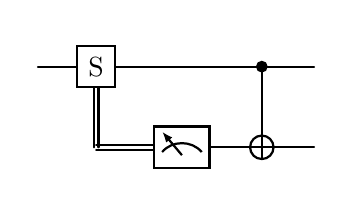
\begin{tikzpicture}
      \node[xscale=-1]{
        \begin{quantikz}[]
          & \ctrl{1} &          &   \gate{\reflectbox{S}} &  \\
          & \targ{}  & \meter{} & \setwiretype{c}\wire[u][1]{c}
        \end{quantikz}
      };
    \end{tikzpicture}
  \end{equation*}
  We read the diagram, according to our convention, from right to left.
  First, we encounter a \(\CNOT\) gate:
  \begin{equation*}
    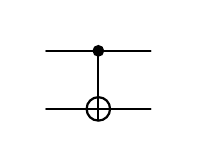
\begin{tikzpicture}
      \node[xscale=-1]{
        \begin{quantikz}[]
          & \ctrl{1} & \\
          & \targ{} &
        \end{quantikz}
      };
    \end{tikzpicture}
  \end{equation*}

  Next, we measure the second qubit in the computational basis:
  \begin{equation*}
    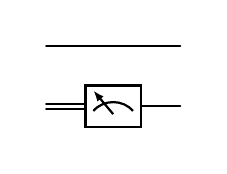
\begin{tikzpicture}
      \node[xscale=-1]{
        \begin{quantikz}[]
          &          &   \\
          & \meter{} & \setwiretype{c}
        \end{quantikz}
      };
    \end{tikzpicture}
  \end{equation*}
The outcome is interpreted as a classical bit: \(0\) if the measurement
outcome was \(\ket{0}\) or \(1\) if \(\ket{1}\) was measured.
The double wire represents this classical information.

Lastly, the connection between this classical wire and the gate \(S\) means that we apply \(S\) only if the measurement outcome was \(1\):
\begin{equation*}
    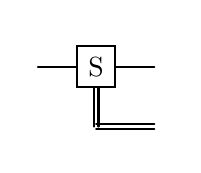
\begin{tikzpicture}
      \node[xscale=-1]{
        \begin{quantikz}[]
          &   \gate{\reflectbox{S}} &  \\
          & \setwiretype{c}\wire[u][1]{c}
        \end{quantikz}
      };
    \end{tikzpicture}
  \end{equation*}

\end{remark}

\cleardoublepage
\subsection{Exercises}\label{sec:basics-exercises}

\subsubsection*{Hilbert spaces}

\begin{exercise}\label{exe:inner-product-is-sesquilinear}
  Show that an inner product \(\braket{\blank}{\bblank} \from V\times V \to \mathbb{C}\) is sesquilinear.

  \textit{Hint:} Use the Hermitian symmetry to move arguments from the first to the second position and vice versa.
\end{exercise}

\begin{exercise}\label{exe:alternative-defn-orthogonal-projection}
  Suppose \(V\) is a Hilbert space.
  Show that a linear map \(f \from V\to V\) is an orthogonal projection onto a subspace \(U \subset V\) if and only if \(f^{2} = f\), \(\im f = U\), and \(\ker f = U^{\perp}\).
\end{exercise}

\begin{exercise}\label{exe:orth-complement-direct-sum}
  Let \(U\subset V\) be a subspace of a finite-dimensional Hilbert space.
  Show that \(U\oplus U^{\perp} = V\) by proceeding as follows.
  \begin{thmlist}
    \item Show that if \(u_{1} + u_{2} = r_{1} + r_{2} \) with \(u_{1}, r_{1} \in U\) and \(u_{2}, r_{2} \in U^{\perp}\) then \(u_{1} = r_{1}\) and \(u_{2} = r_{2}\).

    \textit{Hint:} What is the value of \(\braket{u_{1}-r_{1}}{u_{1} -r_{1}}\)?
    \item Show that \((U+ U^{\perp})^{\perp} =\{0\}\).
    \item Use that \(\{0\}^{\perp} = V\) to conclude the proof.
  \end{thmlist}
\end{exercise}

\begin{exercise}\label{exe:char-of-self-adjoint}
  Let  \(A \in \Mat_{m,n} ( \mathbb{C})\) be a matrix.
  \begin{thmlist}
    \item Show that \(\braket{v}{Aw} = \braket{A^{\dagger} v}{w}\) for all \(v\in \mathbb{C}^{m}\) and \(w \in \mathbb{C}^{n}\).
    \item Suppose now that \(A\) is a \(n\times n\) square matrix.
    Prove that \(A= A^{\dagger}\) if and only if \(\braket{v}{Aw} = \braket{Av}{w}\) for all \( v,w \in \mathbb{C}^{n}\).

    \textit{Hint:} Let \(e_{j}, e_{k}\in \mathbb{C}^{n}\) be two standard basis vectors.
    What is \(\braket{e_{j}}{A e_{k}}\)?
  \end{thmlist}
\end{exercise}



\begin{exercise}\label{exe:unitary-matrix-unitary-map}
  Suppose \(V\) is a Hilbert space with orthonormal basis \(\mathcal{B}\) and \(f\from V\to V\) is a linear map.
  Show that \(f\) is unitary if and only if its transformation matrix is unitary.
\end{exercise}

\begin{exercise}\label{exe:proof-of-lem-canonical-iso-to-dual-space}
  This exercise walks you through a guided proof of Lemma~\ref{lem:canonical-iso-to-dual-space}.
  Consider a finite-dimensional Hilbert space \( V \) and fix an orthonormal basis \( \mathcal{B} = (b_1, \dots, b_n) \) of \( V \).
  \begin{thmlist}
    \item Which axiom of the inner product ensures that \( d \) is well-defined?
    \item Show that \( d(\mathcal{B}) = ( d(b_1), \dots, d(b_n)) \) is a basis of \( \rd*{V}\).
    (Hint: Evaluate \( d(b_i) \) on \( b_j \) for all \( i, j \).)
    \item Use the anti-linearity of \( d \) to conclude that \( d \) is a bijection.
    \item Verify that the given inner product on \( \rd*{V} \) satisfies all axioms of an inner product.
  \end{thmlist}
\end{exercise}

\subsubsection*{States}

\begin{exercise}
  Consider linearly independent vectors \(v, w \in \mathbb{C}^{2}\) such that \( \|v \| = 1 = \|w\|\).
  Prove that \([v]\) and \([w]\) are different states.
\end{exercise}


\begin{exercise}
  The Hadamard gate is modelled by the unitary matrix \(H= \tfrac{1}{2}
  \begin{psmallmatrix}
    1 & 1 \\ 1 & -1
  \end{psmallmatrix} \in \Mat_{2}( \mathbb{C}).
  \)
  Compute \(H\ket{0}\) and \(H \ket{1}\) and determine the associated points on the Bloch sphere.
\end{exercise}

\begin{exercise}
  Find for each Pauli matrix \(\sigma \in\{\sigma_{x}, \sigma_{y}, \sigma_{z}\}\) and normalised eigenvector \(v \in \mathbb{C}^{2}\) of \(\sigma\) the point \(p_{v}\in S^{2}\) on the Bloch sphere associated to the state \([v]\).
\end{exercise}

\begin{exercise}
  Suppose \(v, w \in \mathbb{C}^{2}\) are two normalised vectors such that \(\braket{v}{w}= 0\).
  Let \(p_{v}, p_{w} \in S^{2} \) be the points on the Bloch sphere associated to the states \([v], [w]\).
  Show that \(p_{v} = - p_{w}\).
\end{exercise}

\subsubsection*{Compound systems}
\begin{exercise}\label{exe:bilinear-vs-linear-hom}
  Show that there is a bijection
  \begin{align*}
    \{\text{bilinear maps } V\times W \to X \} & \to \{\text{linear maps} V\to \Hom_{ \mathbb{C}}(W,Z) \} \\
    b & \mapsto (v\mapsto b(v, \blank)) \\
    (B(v) w \longmapsfrom (v,w)) &\longmapsfrom B
  \end{align*}
\end{exercise}


\begin{exercise}\label{exe:translating-bilinear-to-sesquilinear}
  To any vector space \( V \), we assign a new vector space structure on \(V\) with the same vector addition and scalar multiplication defined by
  \begin{equation*}
    \lambda \cdot v \eqdef \overline{\lambda}v \qquad\quad \text{ for all }\lambda \in \mathbb{C}, v\in V.
  \end{equation*}
  To better distinguish between \(V\) and \(\overline{V}\), we write \(\overline{v}\in \overline{V}\) for the corresponding element \(v\in V\).

  Show that a map \( \phi \from V \times V \to \mathbb{C} \) is sesquilinear if and only if the map \( \psi \from \overline{V} \times V \to \mathbb{C} \) defined by \( \psi(\overline{v}, w) = \phi(v, w) \) is bilinear.
\end{exercise}

\begin{exercise}\label{exe:schur-decomposition}
  Given a square matrix \(A\in \Mat_{n}( \mathbb{C})\), show that there is a (unitary) matrix \(P \in \GL_{n}( \mathbb{C})\) such that \(A'= PAP^{-1}\) is upper triangular.
  That is, \((A')_{ij} =0 \) if \(i<j\).

  \textit{Hint:} The diagonal entries of \(A'\) must be the eigenvalues of \(A\) (counted with multiplicities).
\end{exercise}

\begin{exercise}
  Let \(v, v' \in V\) and \(w, w'\in W\) be normalised vectors.
  \begin{thmlist}
    \item Write \((v + v') \otimes (w + w')\) as a linear combination of elementary tensors.
    \item Find a vector in \( \mathbb{C}^{2} \otimes \mathbb{C}^{2}\) that is not an elementary tensor.
    \item Is the vector \(v \otimes w\) normalised?
    Compute its norm.
    \item Compute the Kronecker product \(\sigma_{z} \otimes \sigma_{y}\) (where \(\sigma_{z}, \sigma_{y}\) are Pauli matrices).
    \item Calculate \((\sigma_{z} \otimes \sigma_{y}) \ket{01}\).
    \item What is the rank of \(\sigma_{x}\otimes \sigma_{z}\)?
  \end{thmlist}
\end{exercise}

\begin{exercise}
  Consider a mixed state \(\rho \from V\otimes W \to V\otimes W\) of rank \(1\).
  Show that the corresponding state \(x \in V\otimes W\) is a separable if and only if \(\rho = \sum_{k=1}^{n} \lambda_{k} \phi_{k} \otimes \psi_{k}\) for \(\phi_{k} \from V\to V\) and \(\phi_{k} \from W\to W\) mixed states and real numbers \(\lambda_{k} > 0\) such that \(\sum_{k=1}^{n}\lambda_{k} =1\).

  \textit{Hint:} Show that in the rank \(1\) case we can chose \(n=1\).
  To that end, consider a vector \(x \in V\otimes W\) and compute
  \(\braket{x}{\phi_{k} \otimes \psi_{k} \mid x}\).

  \textit{Hint:} Apply the spectral theorem to show that for any mixed state \(\zeta \from X \to X\) one has \(\zeta(x) = 0\) if and only if \(\braket{x}{\zeta \mid x} = 0\).
\end{exercise}

\begin{exercise}
  Prove for  finite-dimensional vector spaces \(V, W\)  the following identities and represent them as string diagrams.
  \begin{thmlist}
    \item \(\coev_{V} = \tau_{V,\rd*{V}}\widetilde{\coev}_{V}\)
    \item \(\ev_{V} = \widetilde{\ev}_{V}\tau_{V,\rd*{V}}\)
    \item \(\tau_{W,V}\tau_{V,W} = \id_{V,W}\)
  \end{thmlist}
\end{exercise}

\begin{exercise}\label{exe:braid-relations}
  Given vector spaces \(V,W, X\), show that
  \begin{equation*}
    (\tau_{W,X}\otimes \id_{V})(\id_{W}\otimes \tau_{V,W})(\tau_{V,W}\otimes \id_{X})
    =
    (\id_{X}\otimes \tau_{V,W})(\tau_{V,X} \otimes \id_{W})(\id_{V}\otimes \tau_{W,X}).
  \end{equation*}

  Let \(s \from\{1, \dots , n\} \to \{1, \dots , n\}\) be a bijection and \(V_{1}, \dots , V_{n}\) pairwise distinct vector spaces.
  Consider two maps linear maps \(\chi, \zeta \from V_{1} \otimes \dots \otimes V_{n} \to V_{s(1)} \otimes \dots \otimes V_{s(n)}\) which are compositions of tensor flips and  identities.
  Specifically, each component in the composition is of the form
  \begin{equation*}
    \id_{V_1} \otimes \dots \otimes \id_{V_{k-1}} \otimes \tau_{V_k, V_{k+1}} \otimes \id_{V_{k+2}} \otimes \dots \otimes \id_{V_n}.
  \end{equation*}
  Show that  \(\chi = \zeta\).
\end{exercise}

\begin{exercise}
  Let \(f\from V\to W\) be a morphism between finite-dimensional vector spaces.
  Give a string diagrammatic proof of
  \begin{equation*}
    (\id_{\rd*{V}}\otimes f)\coev_{V} = (\rd*{f} \otimes \id_{W})\coev_{W}, \qquad
    \ev_W (f \otimes \id_{\rd*{W}}) = \ev_{V}(\id_{V}\otimes \rd*{f})
  \end{equation*}
\end{exercise}

\begin{exercise}
  Let \(V\), \(W\) be two finite-dimensional vector space.
  \begin{thmlist}
    \item Show that \(\coev_{V\otimes W} = (\id_{V} \otimes \coev_{W}\otimes \id_{\rd*{V}})\coev_{V}\)
    \item Fill in the correct letters such that the following equation holds
    \begin{equation*}
      \widetilde{\ev}_{{V\otimes W}} = (\widetilde{\ev}_{\square})(\square \otimes \widetilde{\ev}_{\square} \otimes \square).
    \end{equation*}

    \item Prove diagrammatically that for any pair of linear maps \(f\from V\to V\) and \(g \from W \to W\), we have \(\tr(f \otimes g) = \tr(f)\tr(g)\).
  \end{thmlist}
\end{exercise}

\begin{exercise}
  Consider morphisms \(f \from V\to W\) and \(g \from W\to X\).
  Show that for the dual morphism, we have
  \(\rd*{(g\circ f)} = \rd*{f} \circ \rd*{g}\).
\end{exercise}

\begin{exercise}
  Given a finite-dimensional vector space \(V\), find, using string diagrams, an isomorphism
  \(\mathrm{dd}\from V \to \rrd*{V}\), where \(\rrd*{V}\) is the dual space of \(\rd*{V}\).
\end{exercise}

\begin{exercise}
  Consider a matrix \(A \in \Mat_{n}( \mathbb{C})\).
  Fill in the box of the following diagram in two different ways to get \(\tr(A)^{2}\), and \(\tr(A^{2})\), respectively.
  \begin{equation*}
    \inputtikz{determinant}
  \end{equation*}
\end{exercise}

\subsubsection*{Unitary transformations}

\begin{exercise}
  Show that for two density matrices \(\rho, \zeta \in \Mat_{n}( \mathbb{C})\) there is a unitary \(U \in \U(n)\) such that \(U\rho U^{\dagger} = \zeta\) if and only if the characteristic polynomials  \(\chi_{\rho}(t)\) and \(\chi_{\zeta}(t)\) are equal.
\end{exercise}

\begin{exercise}
  Compute the Euler decomposition of  \(Y(\gamma)\from \mathbb{C}^{2}\to \mathbb{C}^{2}\) for all \(\gamma \in \mathbb{R}\).
\end{exercise}

\begin{exercise}
  Prove or disprove: given \(\alpha, \beta,\in \mathbb{R}\), there are\(\gamma\in \mathbb{R}\) and \(\lambda \in \mathbb{C}\) such that \(Z(\alpha)X(\beta) - X(\beta) Z(\alpha) = \lambda Y(\gamma)\).
\end{exercise}

\begin{exercise}
  Determine the transformation matrix with respect to the computational basis of \((\mathbb{C}^{2})^{\otimes 2}\) of the map \(UB(\tau) \from (\mathbb{C}^{2})^{\otimes 2} \to (\mathbb{C}^{2})^{\otimes 2}\) associated to the function \(\tau \from \{0,1\}\to\{0,1\}\), \(x \mapsto x \boxplus 1\).
\end{exercise}

\begin{exercise}
  Consider the following unitary matrix:
  \begin{equation*}
    U= \begin{pmatrix}
      1 & 0 & 0 & 0 \\
      0 & 1 & 0 & 0 \\
      0 & 0 & \tfrac{\sqrt{3}}{2}i & \tfrac{1}{2} \\
      0 & 0 & - \tfrac{1}{2} & -\tfrac{\sqrt{3}}{2}i
    \end{pmatrix}.
  \end{equation*}
  Show that there is no map \(f \from\{0,1\}\to\{0,1\}\) and basis \(\mathcal{B}\) of \(( \mathbb{C}^{2})^{\otimes 2}\) such that \(U = {}_{\mathcal{B}}(UB(f))_{\mathcal{B}}\).
\end{exercise}

\begin{exercise}
  Show that for each pair \(\mathcal{B} = (b_{1}, \dots , b_{n})\) and \(\mathcal{C} = (c_{1}, \dots , c_{n})\) of orthonormal bases of \(V\) there is a unitary map \(f \from V\to V\) such that \(f(b_{j}) = c_{j}\) for all \(1 \leq j \leq n\).
\end{exercise}
\subsubsection*{Measurement}

\begin{exercise}
  Let \( V \) be a finite-dimensional Hilbert space and consider \( \End(V) \) as a Hilbert space via the inner product
  \begin{equation*}
    \braket{f}{g} = \tr(f^{\dagger}g).
  \end{equation*}
  Prove that for two \(e_{i}, e_{j}\from V\to V\), we have
  \(e_{i} e_{j} =0 = e_{j} e_{i}\) if and only if \(\braket{e_{i}}{e_{j}} = 0\).

  \textit{Hint:} Let \(\mathcal{B}\) be a (well-chosen) orthonormal basis of \(V\).
  Express \(\tr(e_{i} e_{j})\) using \(\mathcal{B}\) the inner product of \(V\) to conclude that if
  \(\tr(e_{i} e_{j}) =0\) the image of \(e_{i}\) must be contained in the orthogonal complement of the image of \(e_{j}\).
\end{exercise}

\begin{exercise}\label{exe:orthogonal-eigenspaces}
  Consider an observable \(f\from V\to V\) on a finite dimensional Hilbert space, \(\mathrm{spec}(f)= \{\lambda_{1}, \dots , \lambda_{n}\}\) the distinct eigenvalues of \(f\) and \(f = \sum_{i=1}^{n} \lambda_{i} e_{i}\) for \(e_{i} \from V\to V\) the projectors onto the \(i\)-th eigenspaces.
  Show that \(e_{i}e_{j}=0= e_{j}e_{i}\) for \(i \neq j\).
\end{exercise}

\begin{exercise}
  Let \(\Lambda, \Gamma\) be finite sets, \(V, W\) Hilbert spaces and \(E\from\{X \subseteq \Lambda\} \to \mathrm{Proj}(V)\) as well as \(F \from\{Y \subseteq \Gamma\} \to \mathrm{Proj}(W)\) projection-valued measures.
  Show that we have a projection-valued measure
  \begin{equation*}
    \{Z \from \Lambda \times \Gamma\} \to \mathrm{Proj}(V),\qquad Z\mapsto \sum_{(x,y) \in Z} E(x)\otimes F(y).
  \end{equation*}
\end{exercise}

\begin{exercise}
  Let \(e_{1}, e_{2} \from V\to V\) be two orthogonal projectors.
  Prove that their sum is an orthogonal projector if and only if \(e_{1}e_{2}= 0 = e_{2}e_{1}\).
\end{exercise}


\cleardoublepage
\subsection{Study goals}\label{sec:SCUM-study-goals}
The questions below are designed to help you build a conceptual understanding of the SCUM-axioms.
You should aim to answer and explain your reasoning independently, without relying on external aids such as search engines or AI tools.
The level of difficulty is aligned with what you can expect in the exam.

\subsubsection*{Hilbert spaces}
\begin{thmlist}
\item Compute \(\braket{
\begin{psmallmatrix}
2 \\3
\end{psmallmatrix}}{
\begin{psmallmatrix}
5 \\ 2
\end{psmallmatrix}
}_{\mathrm{std}}. \)
\item Find vectors \(v, w \in \mathbb{C}^{3}\) such that \(\braket{v}{w} = 3i\).
\item Suppose \(v\in \mathbb{C}^{3}\) satisifes \(\braket{v}{v}_{\mathrm{std}} = 0\).
What can be said about \(v\)?
\item Let \(U, W\) be \(2\) and \(5\)-dimensional subspaces of a vector space \(V\), respectively.
Whose orthogonal complement has a bigger dimension?
\item Are there scalars \(\lambda, \mu \in \mathbb{C}\) such that
\(\left(
  \lambda
  \begin{psmallmatrix}
    1 \\ 2
  \end{psmallmatrix},
  \mu
  \begin{psmallmatrix}
    -2 \\ 1
  \end{psmallmatrix}
\right)\)
is an orthonormal basis of \( \mathbb{C}^{2}\)?
\item Consider a linear map \(f \from \mathbb{C}^{2} \to \mathbb{C}^{3}\). Is \(ff^{\dagger}\) self-adjoint?
\item Define an orthonormal projection \(e \from \mathbb{C}^{2} \to \mathbb{C}^{2}\) onto
\(\left\{
  \begin{psmallmatrix}
    z \\ - z
  \end{psmallmatrix} \; \middle\vert\; z\in \mathbb{C}
\right\}\).
\item Show that the eigenvalues of a self-adjoint map \(f \from V \to V\) are real.
\item Decide which of the following properties hold for the matrix \(H=
\tfrac{1}{\sqrt{2}}
\begin{psmallmatrix}
  1 & 1 \\ 1 & -1
\end{psmallmatrix}
\):
Is it unitary, self-adjoint, or positive semidefinite? Multiple answers can be true.
\item Let \(\mathcal{B}=(b_{1}, b_{2}, b_{3})\) be a basis of \( \mathbb{C}^{3}\).
Is \((d(b_{1}), d(b_{2}), d(b_{3}))\) a basis of \(\rd*{ \mathbb{C}^{3}}\)?
\end{thmlist}
\subsubsection*{States}
\begin{thmlist}
  \item  Is the vector \( \tfrac{1}{5} \big(3\ket{0} + 4\ket{1}) \in \mathbb{C}^{2}\) normalised?
  \item Calculate the norm of the vector \(\ket 0 + \ket 1\).
  \item Find the complex numbers \(x, y\in \mathbb{C}\) such that \(
  \begin{psmallmatrix}
    x \\ y
  \end{psmallmatrix} = 2\ket{0} - i\ket{1}\).
  \item Do the vectors \(
  \tfrac{1}{\sqrt{2}}
  \begin{psmallmatrix}
    1 \\1
  \end{psmallmatrix}
\) and \( \tfrac{1}{\sqrt{2}}
  \begin{psmallmatrix}
    1 \\-1
  \end{psmallmatrix}\)
  represent the same state?
  \item Write the pure state \(\tfrac{1}{\sqrt{2}}
  \begin{psmallmatrix}
    1 \\1
  \end{psmallmatrix} \in \mathbb{C}^{2}\) as a density matrix \(A \in \Mat_{2}( \mathbb{C})\).
  \item Determine the density matrix associated to the point on the Bloch sphere \((\tfrac{1}{2}, 0, \tfrac{\sqrt{3}}{2})\in S^{2}\).
  \item Does the matrix \(\tfrac{1}{2} \begin{psmallmatrix} 1 & 0 \\ 0 & 1 \end{psmallmatrix}\) represent the density matrix of a pure state?
  \item Consider a density matrix \(M \in \Mat_{n}( \mathbb{C})\). What can be said about its eigenvalues?
\end{thmlist}
\subsubsection*{Compound systems}
\begin{thmlist}
  \item Suppose \(X= V\otimes W\) is an \(11\)-dimensional vector space. What can you say about the dimensions of \(V\) and \(W\)?
  \item Is the map \(\mu \from \mathbb{C} \times \mathbb{C} \to \mathbb{C}\), \((w,z) \mapsto wz\) bilinear?
  \item Simplify the sum \(
  \begin{psmallmatrix}
    1 \\ 0
  \end{psmallmatrix} \otimes
  \begin{psmallmatrix}
     0 \\ 1
  \end{psmallmatrix}
  +
  \begin{psmallmatrix}
    1 \\ 0
  \end{psmallmatrix} \otimes
  \begin{psmallmatrix}
    1 \\ 0
  \end{psmallmatrix}
\).
  \item Compute the Kronecker product \(\sigma_{z}\otimes \sigma_{z}\) for the Pauli matrix \(\sigma_{z}\).
  \item Find examples for states in \( \mathbb{C}^{2}\otimes \mathbb{C}^{2}\) that are  a product state, entangled, and in a superposition with respect to the computational basis (\(\ket{00},\ket{01}, \ket{10}, \ket{11}\)), respectively.
  \item Consider normalised vectors \(v, v', w, w' \in \mathbb{C}^{2}\) such that \([v]=[v']\) as well as  \([w]=[w']\) represent the same state.
  Explain this equivalence relation explicitly.
  Then show that \([v\otimes w] = [v' \otimes w']\) needs not hold.
  \item Let \(A , B \in \Mat_{2}( \mathbb{C})\) have integer eigenvalues.
  Are the eigenvalues of \(A\otimes B\) integers?
  \item Compute the length of \(\ket{00} + \ket{01} \in \mathbb{C}^{2}\).
  \item Consider the following matrix
  \begin{equation*}
      A=\begin{pmatrix}
    1 & 0 & 0 & 0 \\
    0 & 1 & 0 & 0 \\
    0 & 0 & 0 & 1 \\
    0 & 0 & 1 & 0
  \end{pmatrix} \in \Mat_{4}(\mathbb{C}).
\end{equation*}
  Why are there no matrices \(B, C \in \Mat_{2}( \mathbb{C})\), such that \(A= B\otimes C\)?
  \item Compute the partial trace \(\mathrm{Tr}_{ \mathbb{C}^{2}, \mathbb{C}^{2}}^{ \mathbb{C}^{2}}(A)\) (with respect to the second tensor factor) of the matrix \(A\) of the previous question.
  \item Prove string diagramatically: If \(f \from V \to W\) and \(g \from X \to Y\) are isomorphisms, then \(f\otimes g \from V\otimes X \to W\otimes Y\) is an isomorphism as well.
  \item Find a string diagram (only using crossings) that represents the map \(V^{\otimes 3}\to V^{\otimes 3}\),
  \(v\otimes w \otimes x \mapsto x \otimes w \otimes v\).
\end{thmlist}

\subsubsection*{Unitary transformations}
\begin{thmlist}
  \item Show that any eigenvalue \(\lambda \in \mathbb{C}\) of a unitary transformation \(f \from V\to V\) must satisfy \(|\lambda| = 1\).
  \item Determine a unitary map \(f\from \mathbb{C}^{2} \to \mathbb{C}^{2}\) such that \(f (\ket{0}\bra{0}) f^{\dagger} = \ket{+}\bra{+}\).
  \item Explain the induced rotation on the Bloch sphere of the map \(Z(\tfrac{1}{4}) X(\tfrac{1}{4}) Z(\tfrac{1}{4})\).
  \item What is the unitary map \(UB(f) \from (\mathbb{C}^{2})^{\otimes 3}\to (\mathbb{C}^{2})^{\otimes 3}\) corresponding by Bennett's trick to \(f \from\{0,1\} \to\{0,1\}^{2}\), \(x \mapsto (x, x)\).
\end{thmlist}

\subsubsection*{Measurement}
\begin{thmlist}
  \item Let \(e_{1}, e_{2} \from V\to V\) be orthogonal projections. Does \(e_{1} e_{2} = 0 \) imply \(e_{2} e_{1}=0\)?
  \item Define the projection-valued measure associated to the positive self-adjoint matrix \(
  \begin{pmatrix}
    2 & -1 \\  -1 & 2
  \end{pmatrix}
  \).
  \item Given the projection \(e_{1} \from \mathbb{C}^{2} \to \mathbb{C}^{2}\), \(
  \begin{psmallmatrix}
    x\\ y
  \end{psmallmatrix}
  \mapsto \tfrac{1}{2}
  \begin{psmallmatrix}
    x + y \\ x + y
  \end{psmallmatrix},
  \)
  find, with respect to the standard basis, the transformation matrix of the projection \(e_{2} \from \mathbb{C}^{2} \to \mathbb{C}^{2}\) such that \(e_{1} + e_{2} = \id_{ \mathbb{C}^{2}}\).
  \item With \(e_{1}\) and \(e_{2}\) as before. What are the images of \(e_{1}\) and \(e_{2}\)?
  \item Consider the Hilbert space \( \mathbb{C}^{2}\) and let \(\Lambda =\{0,1\}\) and the projection-valued measure \( E \from\{X \subseteq \Lambda\} \to \mathrm{Proj}(V)\) be defined by \(E(\{0\}) =e_{0}\) and \(E(\{1\}) =e_{1}\), where \(e_{0}, e_{1} \from \mathbb{C}\to \mathbb{C}\) are the orthogonal projections onto \(\{\lambda \ket{0} \mid \lambda \in \mathbb{C}\}\) and \(\{ \lambda \ket{1} \mid \lambda \in \mathbb{C}\}\), respectively.
  What is the probability of observing the outcome \(\{1\}\) upon measuring for the state \(\ket{+}\)?
 \item Retain the notion of the previous question. Suppose we observed  the outcome \(\{1\}\) for the state \(\ket{+}\). What is the updated state?
\end{thmlist}


\cleardoublepage
\part{Quantum algorithms and the ZX-calculus}
\section{Quantum computation via the ZX-calculus}\label{sec:quantum-computation-via-the-zx-calculus}

The ZX-calculus is a variant of the string diagrammatic calculus.
The following quote, taken from the website \url{https://zxcalculus.com/} describes its applications and purposes.

\begin{quote}
  The ZX-calculus is a graphical language that goes beyond circuit diagrams.
  It ``splits the atom'' of well-known quantum logic gates to reveal the compositional structure inside.
  The calculus works by generalising the ideas of Z and X operations, allowing us to break out of the circuit model while maintaining soundness of reasoning.
  In doing so we can show properties of circuits, entanglement states, and protocols, in a visually succinct but logically complete manner.

  The ZX-calculus is forging the next generation of quantum software.
  Using the calculus gives optimisation strategies that performs state-of-the-art T-count reduction (an important metric for fault-tolerant computing) and gate compilation.
  The generators of the calculus correspond closely to the basic operations of lattice surgery in the surface code, giving a visual design and verification language for these codes; and ZX has also been used to discover novel error correction procedures.
  It comes with a scalable notation capable of representing repeated structures at arbitrary qubit scales. (...)
\end{quote}

The ZX-calculus is discussed in detail in \cite[Chapter~3]{kissinger-wetering2025:PicturingQuantumSoftware} and \cite{coecke-kissinger2017:PicturingQuantumProcesses}.
\subsection{ZX-spiders}\label{sec:zx-spiders}
The ZX calculus builds on the observation that any unitary matrix can be written as a product of \(Z\) and \(X\) phase gates (up to a global phase), and extends this to a language suitable for diagrammatically reasoning about arbitrary linear maps.

\begin{convention}
  For the \(ZX\)-calculus, we agree on the following conventions.
  \begin{thmlist}
    \item We identify the vector spaces \( \rd*{\mathbb{C}}\) and \(\mathbb{C}\) using the isomorphism
    \begin{equation*}
       \rd*{ \mathbb{C}} \to \mathbb{C}, \qquad \lambda \mapsto \lambda(1).
    \end{equation*}
    \item We identify the vector spaces \( \rd*{\mathbb{C}^{2}}\) and \(\mathbb{C}^{2}\) using the unique isomorphism \(\rd*{\mathbb{C}^{2}} \to \mathbb{C}^{2}\) that satisfies
    \begin{equation*}
       \bra{0} \mapsto \ket{0}, \qquad \bra{1} \mapsto \ket{1}.
    \end{equation*}
    \item We set
    \begin{equation*}
      \ket{0}^{\otimes 0} = 1 = \ket{1}^{\otimes 0}, \qquad
      \ket{+}^{\otimes 0} = 1 = \ket{-}^{\otimes 0}.
    \end{equation*}
  \end{thmlist}
\end{convention}

These conventions have immediate consequences for our string diagrams.
From now on, we will simply write
\begin{equation*}
  \inputtikz{zx-conventions}
\end{equation*}


\begin{definition}\label{def:zx-spiders}
  Given natural numbers \( n, m \in \mathbb{N}_{0} \) and \( \alpha, \beta \in \mathbb{R} \), we define the \emph{Z-spider} \( Z_n^m(\alpha) \) and the \emph{X-spider} \( X_n^m(\beta) \) as the linear maps
  \begin{subequations}
    \begin{align}
      Z_{n}^{m}(\alpha) &= \ket{0}^{\otimes m}\bra{0}^{\otimes n} + e^{2\pi i \alpha}\ket{1}^{\otimes m} \bra{1} ^{\otimes n}\from ( \mathbb{C}^{2})^{\otimes n} \to ( \mathbb{C}^{2})^{\otimes m}, \\
      X_{n}^{m}(\beta) &= \ket{+}^{\otimes m}\bra{+}^{\otimes n} + e^{2\pi i \beta}\ket{-}^{\otimes m} \bra{-} ^{\otimes n}\from ( \mathbb{C}^{2})^{\otimes n} \to ( \mathbb{C}^{2})^{\otimes m}
    \end{align}
  \end{subequations}
  The spiders \(Z_{n}^{m}(\alpha)\) and  \(X_{n}^{m}(\beta)\) are operations of \emph{arity} \((n,m)\) with \(n\) \emph{inputs} and  \(m\) outputs.

  In case \(\alpha, \beta \in \mathbb{Z}\) are integers, we call \(Z_{n}^{m}(\alpha)\), respectively \(X_{n}^{m}(\beta)\) \emph{phase-free} and write \(Z_{n}^{m} \eqdef Z_{n}^{m}(\alpha)\) as well as \(X_{n}^{m} \eqdef X_{n}^{m}(\beta)\).
\end{definition}

We draw \(Z\) and \(X\)-spiders of arity \((n,m)\) as coloured boxes with \(n\) incoming and \(m\) outgoing strings.
Here the strings are undirected.
\begin{equation*}
  \inputtikz{zx-examples}
\end{equation*}

The states below are named after the physicists Greenberger, Horne, and Zeilinger
\footnote{The below short biographies are taken from their wikipedia pages:
  \begin{thmlist}
    \item Daniel M. Greenberger is an American quantum physicist. He has been professor of physics at the City College of New York since 1964.
    \item Michael Allan Horne (January 18, 1943 -- January 19, 2019) was an American quantum physicist, known for his work on the foundations of quantum mechanics.
    \item Anton Zeilinger (born 20 May 1945) is an Austrian quantum physicist and Nobel laureate in physics of 2022.
  \end{thmlist}
}.
\begin{definition}\label{def:GHZ-states}
  Let \(m \geq 2\) be a natural number.
  The \emph{GHZ state}  for \( m \) qubits is
  \begin{equation}\label{eq:GHZ-state}
    \ket{\textrm{GHZ}_m} = \frac{1}{\sqrt{2}} \left( \ket{0}^{\otimes m} + \ket{1}^{\otimes m} \right).
  \end{equation}
  For \( m = 2 \), this coincides with  the Bell state \( \ket{\Phi^+} = \frac{1}{\sqrt{2}} (\ket{00} + \ket{11}) \).
\end{definition}
GHZ states can be obtained by  using \(Z\) spiders
\begin{equation}
  Z_0^m(0)\;\tfrac{1}{\sqrt{2}}
  = \frac{1}{\sqrt{2}}\big(\ket{0}^{\otimes m} + \ket{1}^{\otimes m}\big)= \ket{\text{GHZ}_m}, \qquad m \geq 2.
\end{equation}
In case \(m=1\), we obtain
\begin{equation*}
  Z_{0}^{1}(0) \; \tfrac{1}{\sqrt{2}}
  = \frac{1}{\sqrt{2}}\big( \ket{0} + \ket{1})
  = \ket{+},
  \qquad
  Z_{0}^{1}(\tfrac{1}{2}) \; \tfrac{1}{\sqrt{2}}
  =\frac{1}{\sqrt{2}}\big(\ket{0} - \ket{1}\big)
  = \ket{-}
\end{equation*}

On the other hand the spider \( X_0^m\) can be used to create a superposition with respect to the computational basis. Given \(x = (x_{1}, \dots , x_{m})\in\{0,1\}^{m}\), we write \((-1)^{|x|} \eqdef (-1)^{x_{1}+ \dots + x_{m}}\) and observe
\begin{equation*}
  X_0^m(0)\;1
  = \ket{+}^{\otimes m} + \ket{-}^{\otimes m}
  = \left( \frac{1}{\sqrt{2}} \right)^m \sum_{x \in \{0,1\}^m} 1 + (-1)^{|x|}\ket{x},\qquad  m \geq 2.
\end{equation*}
Moreover, we have
\begin{equation*}
  X_{0}^{1}(0)\;\tfrac{1}{\sqrt{2}}
  = \frac{1}{\sqrt{2}}\big(\ket{+} + \ket{-}\big)
  = \ket{0},
  \qquad
  X_{0}^{1}(\tfrac{1}{2})\;\tfrac{1}{\sqrt{2}}
  = \frac{1}{\sqrt{2}}\big(\ket{+} - \ket{-}\big)
  = \ket{1}.
\end{equation*}

\begin{remark}\label{rmk:x-creates-z-and-vice-versa}
  By the above computations, we get the \(Z\)-basis from \(X\)-spiders, and the \(X\)-basis from the \(Z\)-spiders.
  \begin{equation*}
    \inputtikz{ZX-basis-creation}
  \end{equation*}
\end{remark}
\subsubsection{Classical gates from ZX-diagrams}\label{sec:classical-gates-from-zx-diagrams}
Before developing the syntax of the ZX-calculus---in form of rewriting rules---and
formally defining ZX-diagrams, we aim to build our intuition for the kinds of maps that can be expressed by composing and tensoring \( Z \)- and \( X \)-spiders.
In particular, we will discuss the \(ZX\)-representation of the quantum gates covered in Section~\ref{sec:quantum-circuits}.
\bigskip

For now, we will use the term ``ZX-diagram'' to refer to a string diagram whose nodes are either \(Z\) or \(X\)-spiders.
Some examples of such diagrams are shown below.
\begin{equation} \label{eq:ZX-closed-examples}
  \inputtikz{ZX-closed-examples}
\end{equation}

\begin{lemma}\label{lem:any-complex-number}
  For any complex number \(z\in \mathbb{C}\), there exists a \(ZX\)-diagram representing this number.
\end{lemma}
\begin{proof}
  A guided step-by-step approach to the proof is given in Exercise~\ref{exe:complex-numbers-as-ZX-diagrams}.
\end{proof}
\bigskip

\noindent
\textbf{The Z-gate}: The \(Z\)-phase gate \(Z(\alpha) \from \mathbb{C}^{2}\to \mathbb{C}^{2}\) simply corresponds to  \(Z_{1}^{1}(\alpha)\), where \(\alpha \in \mathbb{R}\) is a real parameter.
\bigskip

\noindent
\textbf{The X-gate}: For any \(\beta \in \mathbb{R}\), the \(X\)-phase gate \(X(\beta) \from \mathbb{C}^{2}\to \mathbb{C}^{2}\) coincides with \(X_{1}^{1}(\beta)\).
\bigskip

\noindent
\textbf{The CNOT-gate}: The \(\CNOT\) is obtained by composing multiple \(X\)- and \(Z\)-spider.
We will derive two presentations.
Both rely on the next auxiliary lemma that uses the addition modulo \(2\) discussed in Remark~\ref{rem:addition-modulo-2}.

\begin{lemma}\label{lem:CNOT-auxiliary-XZ}
  Given \(a, b,c \in\{0,1\}\), we obtain
  \begin{subequations}
    \begin{align}
      Z_{1}^{2} \ket{a}  = \ket{aa}, \qquad
      Z_{2}^{1} \ket{bc} = \delta_{b=c}\ket{b} \label{eq:Z21-and-Z12-gates}\\
      X_{1}^{2} \ket{a}  = \tfrac{1}{\sqrt{2}} \sum_{k=0}^{1} \ket{k}\otimes \ket{a \boxplus k}, \qquad
      X_{2}^{1} \ket{bc} = \tfrac{1}{\sqrt{2}}(\ket{b \boxplus c}) \label{eq:X21-and-X12-gates}
    \end{align}
  \end{subequations}
\end{lemma}
\begin{proof}
  Equation~\eqref{eq:Z21-and-Z12-gates} follows from a straightforward computation.
  To prove Equation~\eqref{eq:X21-and-X12-gates}, we fix \(a, b,c \in\{0,1\}\) and calculate
  \begin{align*}
    \braket{+}{a} = \tfrac{1}{\sqrt2}, \qquad
    \braket{-}{a} = (-1)^{a} \tfrac{1}{\sqrt{2}},
    \qquad
    \ket{++} + (-1)^{a} \ket{--} = \big(\sum\nolimits_{k=0}^{1} \ket{k} \otimes \ket{k \boxplus a}\big), \\
    \braket{+\!+\!}{bc} = \tfrac{1}{2}, \qquad
    \braket{-\!-\!}{bc} = \tfrac{1}{2} (-1)^{b+c},\qquad
    \ket{+} + (-1)^{b+c} \ket{-} = \sqrt{2}\ket{b \boxplus c}
  \end{align*}
  Leading to
  \begin{align*}
    X_{1}^{2}\ket{a}
    & = \ket{++}\braket{+}{a} + \ket{--}\braket{-}{a}
      = \tfrac{1}{\sqrt{2}}\big(\ket{++} + (-1)^{a} \ket{--}\big)
      = \tfrac{1}{\sqrt{2}} \big(\sum\nolimits_{k=0}^{1} \ket{k} \otimes \ket{k \boxplus a}\big), \\
    X_{2}^{1}\ket{bc}
    & = \tfrac{1}{2}\big(\ket{+} + (-1)^{b+c}\ket{-}\big)
      = \tfrac{\sqrt{2}}{2}(\ket{b \boxplus c})
      = \tfrac{1}{\sqrt{2}}(\ket{b \boxplus c})\qedhere
  \end{align*}
\end{proof}


The \(\CNOT\) gate can be characterised as the unique linear map \( (\mathbb{C}^{2})^{\otimes 2} \to (\mathbb{C}^{2})^{\otimes 2}\) satisfying
\begin{equation*}
  \CNOT\ket{ab} = \ket{a} \otimes \ket{a \boxplus b} \qquad \text{ for all } a,b \in\{0,1\}.
\end{equation*}
\begin{lemma}\label{lem:CNOT-equal-presentations}
  We have
  \begin{equation*}
    \inputtikz{ZX-CNOT-variants}
  \end{equation*}
\end{lemma}
\begin{proof}
  Consider \(a ,b \in\{0,1\}\).
  Using Lemma~\ref{lem:CNOT-auxiliary-XZ}, we compute for the left diagram
  \begin{align*}
    (Z_{2}^{1}\otimes \id_{ \mathbb{C}^{2}})(\id_{ \mathbb{C}^{2}} \otimes X_{1}^{2}) \ket{ab}
    & = \tfrac{1}{\sqrt{2}} \sum_{k=0}^{1} (Z_{2}^{1}\otimes \id_{ \mathbb{C}^{2}}) \ket{ak} \otimes \ket{b \boxplus k}
      = \tfrac{1}{\sqrt{2}} \ket{a} \otimes \ket{b \boxplus a}
  \end{align*}
    Similarly, the right diagram yields
  \begin{align*}
    (\id_{ \mathbb{C}^{2}} \otimes X_{2}^{1})(Z_{1}^{2} \otimes \id_{ \mathbb{C}^{2}}) \ket{ab}
    & = (\id_{ \mathbb{C}^{2}} \otimes X_{2}^{1})\ket{aab}
      = \tfrac{1}{\sqrt{2}} \ket{a}\otimes \ket{a \boxplus b}. \qedhere
  \end{align*}
\end{proof}

The previous Lemma allows us to use the following shorthand notation.
\begin{equation*}
  \inputtikz{ZX-pre-CNOT}
\end{equation*}
Combining Lemma~\ref{lem:CNOT-equal-presentations} with Equation~\eqref{eq:ZX-closed-examples} yields a presentation of the CNOT-gate in terms of \(ZX\)-diagrams.
\begin{corollary}\label{cor:CNOT-as-ZX-diagram}
  The CNOT-gate \(\CNOT\from (\mathbb{C}^{2})^{\otimes 2} \to (\mathbb{C}^{2})^{\otimes 2}\) corresponds to the \(ZX\)-diagram
  \begin{equation}\label{eq:ZX-version-of-CNOT}
    \inputtikz{ZX-CNOT}
  \end{equation}
\end{corollary}
\bigskip

\noindent
\textbf{The SWAP gate:}
The SWAP gate interchanges the tensorands of a 2 qubit system.
That is, it maps a  vector \(\ket{ab}\) to \(\ket{ba}\).
We observe that \(\CNOT \ket{ab} = \ket{a} \otimes \ket{a \boxplus b}\) for  \(a, b \in\{0,1\}\), and therefore  transfers at least partially ``information'' from the first to the second qubit.
This suggests that we can use chains of CNOTs to implement the SWAP-gate.

\begin{proposition}\label{prop:swap-as-zx}
  The SWAP-gate \(\SWAP \from ( \mathbb{C}^{2})^{\otimes 2} \to ( \mathbb{C}^{2})^{\otimes 2}\) corresponds to the diagram
  \begin{equation}\label{eq:zw-swap}
    \inputtikz{ZX-SWAP}
  \end{equation}
\end{proposition}
\begin{proof}
  We observe that we can decompose the Diagram~\eqref{eq:zw-swap} into three components: the leftmost and rightmost being CNOT-gates and the middle one a flipped version of the CNOT-gate.
  \begin{equation*}
    \inputtikz{ZX-SWAP-aux}
  \end{equation*}
  Writing \(\sigma\from (\mathbb{C}^{2})^{\otimes 2} \to (\mathbb{C}^{2})^{\otimes 2}\) for the tensor flip, we compute for any \(a, b \in\{0,1\}\)
  \begin{align*}
    (\CNOT\circ (\sigma \CNOT \sigma)\circ \CNOT)\ket{ab}
    & = (\CNOT\circ (\sigma \CNOT \sigma)) \ket{a} \otimes \ket{a \boxplus b}\\
    & = \CNOT \ket{a \boxplus a \boxplus b} \otimes \ket{a \boxplus b}
      = \CNOT \ket{b} \otimes \ket{a \boxplus b}\\
    & = \ket{b} \otimes \ket{a \boxplus b \boxplus b}
      = \ket{ba}. \qedhere
  \end{align*}
\end{proof}
\bigskip

\noindent
\textbf{The Hadamard gate:}
The Hadamard gate, due to its ubiquitous applications,  plays a special role in the \(ZX\)-calculus.
Since it is a unitary operation on a single qubit, we could derive a \(ZX\)-diagram using its Euler decomposition.
\begin{equation}\label{eq:Hadamard-via-Euler-decomposition}
  \inputtikz{ZX-Hadamard-realisation-Euler}
\end{equation}
\begin{proposition}\label{prop:Hadamard-ZX}
  The Hadamard gate \(H \from \mathbb{C}^{2}\to \mathbb{C}^{2}\),
  \(\begin{psmallmatrix}
    x \\ y
  \end{psmallmatrix}\mapsto
  \tfrac{1}{\sqrt{2}}
  \begin{psmallmatrix}
    x+y \\ x-y
  \end{psmallmatrix}\), corresponds to the diagram
  \begin{equation}
    \inputtikz{ZX-Hadamard-realisation}
  \end{equation}
\end{proposition}
\begin{proof}
  The claim follows from a straightforward computation using Lemma~\ref{lem:CNOT-auxiliary-XZ}:
  \begin{align*}
    \big((Z_{1}^{0}(-\tfrac{1}{4})
    & \otimes Z_{1}^{1}(\tfrac{1}{4})) \circ X_{1}^{2} \circ Z_{1}^{1}(\tfrac{1}{4})\big)\ket{0}
      = \big((Z_{1}^{0}(-\tfrac{1}{4}) \otimes Z_{1}^{1}(\tfrac{1}{4})) \circ X_{1}^{2}\big)\ket{0} \\
    & = \tfrac{1}{\sqrt{2}}\big(Z_{1}^{0}(-\tfrac{1}{4}) \otimes Z_{1}^{1}(\tfrac{1}{4})\big) \ket{00} + \ket{11}
      = \tfrac{1}{\sqrt{2}}(\ket{0} + \ket{1}) = \ket{+}   \\
    \big((Z_{1}^{0}(-\tfrac{1}{4})
    & \otimes Z_{1}^{1}(\tfrac{1}{4})) \circ X_{1}^{2} \circ Z_{1}^{1}(\tfrac{1}{4})\big)\ket{1}
      = i \big((Z_{1}^{0}(-\tfrac{1}{4}) \otimes Z_{1}^{1}(\tfrac{1}{4})) \circ X_{1}^{2}\big)\ket{1} \\
    & = \tfrac{i}{\sqrt{2}}\big(Z_{1}^{0}(-\tfrac{1}{4}) \otimes Z_{1}^{1}(\tfrac{1}{4})\big) \ket{01} + \ket{10}
      = \tfrac{i}{\sqrt{2}}(-i\ket{0} + i\ket{1}) = \ket{-}
  \end{align*} \qedhere
\end{proof}

Due to its ubiquity in our quantum algorithms, we add the Hadamard gate as an additional spider to our calculus.

\begin{definition}\label{def:Hadamard-ZX}
  The \emph{Hadamard-spider} is the unitary map
  \begin{equation}
    H \from \mathbb{C}^{2}\to \mathbb{C}^{2}, \qquad
    \begin{pmatrix}
      x \\ y
    \end{pmatrix}\mapsto
    \tfrac{1}{\sqrt{2}}
    \begin{pmatrix}
      x+y \\ x-y
    \end{pmatrix},
  \end{equation}
  which we draw in the \(ZX\)-calculus as a yellow square.
  \begin{equation*}
    \inputtikz{ZX-Hadamard}
  \end{equation*}
\end{definition}

\subsubsection{Interlude: The Deutsch--Jozsa algorithm}\label{sec:interlude:-the-deutsch--jozsa-algorithm}

The \emph{Deutsch--Jozsa algorithm}\footnote{%
  The Deutsch--Jozsa algorithm is named after the physicists
  \textit{David Deutsch} (born 1953) and \textit{Richard Jozsa} (born 1953).
} addresses the following problem:
\begin{center}
  Given a map \( f \from \{0,1\}^m \to \{0,1\} \) that is either
  \begin{thmlist}
    \item \textit{constant}: \( f(x) = f(y) \) for all \( x, y \in \{0,1\}^m \), or
    \item \textit{balanced}: \( |\left\{ x \in \{0,1\}^m \mid f(x) = 0 \right\}| = |\left\{ y \in \{0,1\}^m \mid f(y) = 1 \right\}| \),
  \end{thmlist}
  decide whether \( f \) is balanced or constant.
\end{center}

\noindent
\textbf{The classical approach:}
In the worst case\footnote{This worst-case scenario occurs, for example, if \( f \) is constant.}, we must evaluate \( f \) for at least \( 2^{m-1} + 1 \) inputs to determine whether it is balanced or constant.
\bigskip

\noindent
\textbf{The quantum approach:}
Assume we have a quantum version of our function \(f\) given by the unitary map \( UB(f) \from (\mathbb{C}^2)^{\otimes m+1} \to (\mathbb{C}^2)^{\otimes m+1} \) of \( f \), satisfying (as discussed with Bennett's trick in Section~\ref{sec:translating-classical-algorithms-to-quantum-algorithms})
for every \( x_1, \dots, x_m, y \in \{0,1\} \):
\begin{equation*}
  \ket{x_1 \dots x_m} \otimes \ket{y} \mapsto \ket{x_1 \dots x_m} \otimes \ket{f(x_1, \dots, x_m) \boxplus y}.
\end{equation*}

We will now show that a deceptively simple quantum algorithm can solve this problem. Theorem~\ref{thm:ZX-calculus-is-universal} will show that there even is a ZX-diagram representing \( UB(f) \).
We will use it as a black box and consider the diagram below.
\begin{equation*}
  \inputtikz{Deutsch-Jozsa}
\end{equation*}
Here \(\zeta_{1}= (\tfrac{1}{\sqrt{2}})^{m+1}= \zeta_{2}\) are scalars needed to ensure that we work with normalised vectors.
These scalars can be drawn in the ZX-calculus, see Lemma~\ref{lem:any-complex-number}.

To understand why this can detect whether \( f \) is balanced, we analyse all three phases of the algorithm---state initialisation, quantum circuit application, and measurement—in detail.
\medskip

\noindent
\textit{State initialisation:}
By Remark~\ref{rmk:x-creates-z-and-vice-versa}, a phase-free \( X_0^1 \)-gate creates the state \( \sqrt{2}\ket{0} \), and \( X_0^1(\tfrac{1}{2}) \) gives rise to \( \sqrt{2}\ket{1} \).
Thus, using the normalisation given by the scalar \(\zeta_{1}\), our initial state is
\begin{equation*}
  v_{\text{init}} = \ket{0 \dots 0 1}.
\end{equation*}
\medskip


\noindent
\textit{Quantum circuit:}
The Hadamard gate \( H \from \mathbb{C}^2 \to \mathbb{C}^2 \) corresponds to the change of basis sending \( \ket{0} \) to \( \ket{+} \) and \( \ket{1} \) to \( \ket{-} \).
For any \( x \in \{0,1\} \), we have
\begin{equation}\label{eq:Hadamard-equiv-descriptions}
  H \ket{x} = \frac{1}{\sqrt{2}} \left( \ket{0} + (-1)^x \ket{1} \right) = \frac{1}{\sqrt{2}} \sum_{y \in \{0,1\}} (-1)^{xy} \ket{y}.
\end{equation}

Thus, step 1 of our quantum circuit yields
\begin{equation*}
  v_{\text{step 1}}
  = H^{\otimes m+1} (v_{\text{init}})
  = \left( \frac{1}{\sqrt{2}} \right)^{m+1} \sum_{s \in \{0,1\}^m} \ket{s} \otimes \left( \ket{0} - \ket{1} \right).
\end{equation*}

In order to evaluate \(UB(f) v_{\text{step 1}}\), we compute for a given \( s \in \{0,1\}^m \) the value
\begin{equation*}
  UB(f) \left( \ket{s} \otimes \left( \ket{0} - \ket{1} \right) \right) =
  \begin{cases}
    \ket{s} \otimes \left( \ket{0} - \ket{1} \right) & \text{if } f(s) = 0, \\
    \ket{s} \otimes \left( \ket{1} - \ket{0} \right) & \text{if } f(s) = 1.
  \end{cases}
\end{equation*}
This can also be written as
\begin{equation*}
  UB(f) \left( \ket{s} \otimes \left( \ket{0} - \ket{1} \right) \right) = (-1)^{f(s)} \ket{s} \otimes \left( \ket{0} - \ket{1} \right)
\end{equation*}
and so
\begin{equation*}
  v_{\text{step 2}}
  = UB(f)(v_{\text{step 1}})
  = \left( \frac{1}{\sqrt{2}} \right)^{m+1} \sum_{s \in \{0,1\}^m} (-1)^{f(s)} \ket{s} \otimes \left( \ket{0} - \ket{1} \right).
\end{equation*}
For \( s, z \in \{0,1\}^m \), we write \( sz \eqdef s_1 z_1 + \dots + s_m z_m \).
Then, using the Hadamard transformation, we get
\begin{equation*}
  v_{\text{step 3}}
  = (H^{\otimes m} \otimes \id_{\mathbb{C}^2}) v_{\text{step 2}}
  = \left( \frac{1}{2} \right)^m \sum_{s, z \in \{0,1\}^m} (-1)^{f(s) + sz} \ket{z} \otimes \left( \frac{1}{\sqrt{2}} \big( \ket{0} - \ket{1} \big) \right).
\end{equation*}
\medskip

\noindent
\textit{Measurement:}
Finally, we measure our results.
In the circuit drawn above, this is done by placing at the end of each string either a phase-free \( X_1^0 \)-spider or the \( Z_1^0(\tfrac{1}{2}) \)-spider.
Note that by definition
\begin{equation*}
  X_1^0(0) = \bra{+} + \bra{-} = \sqrt{2} \bra{0}, \quad Z_1^0\left(\tfrac{1}{2}\right) = \bra{0} - \bra{1} = \sqrt{2} \bra{-}.
\end{equation*}

Thus, due to the rescaling factor \(\zeta_{2}\), our measurement map is
\begin{equation*}
  \bra{0}^{\otimes m} \otimes \bra{-}.
\end{equation*}

Let \(\lambda\in \mathbb{C}\) be the the unique scalar such that \(e(v_{\text{step 3}})= \lambda \ket{0}^{\otimes m} \otimes \ket{-} + v^{\perp}\), where \(v^{\perp}\) is orthogonal to \(\ket{0}^{\otimes m} \otimes \ket{-}\).
Then
\begin{equation*}
  \big(\bra{0}^{\otimes m} \otimes \bra{-} \big)v_{\text{step 3}} = \lambda.
\end{equation*}
This is not exactly the projective measurement discussed in Section~\ref{sec:measurements-and-the-born-rule}, but the difference is negligible:
given the projection map  \( e \from (\mathbb{C}^2)^{\otimes m+1} \to (\mathbb{C}^{2})^{\otimes m+1} \) into the subspace spanned by \( \ket{0}^{\otimes m} \otimes \ket{-} \) , we compute the probability of observing our system in state \(\ket{0}^{\otimes m}\otimes \ket{-}\) as
\begin{align*}
  \braket{v_{\text{step 3}}}{ e | v_{\text{step 3}}}
  & = \braket{v_{\text{step 3}}}{ e^{\dagger} e | v_{\text{step 3}}}
    = \braket{e(v_{\text{step 3}})}{e(v_{\text{step 3}})}
    = |\lambda|^{2}.
\end{align*}
Thus, we get the probability of our system being the configuration \(\ket{0}^{\otimes m}\otimes \ket{-}\) as
\begin{equation*}
  |\lambda|^{2}
  = \bigg| \big(\bra{0}^{\otimes m} \otimes \bra{-} \big)v_{\mathrm{step 3}} \bigg|^{2}
  =
  \begin{cases}
    1 & \text{if } f \text{ is constant}, \\
    0 & \text{if } f \text{ is balanced}.
  \end{cases}
\end{equation*}

\subsubsection{Further basic identities of ZX-spiders}\label{sec:further-basic-identities-of-zx-spiders}
With respect to the computational bases of \( (\mathbb{C}^{2})^{\otimes n} \) and \( (\mathbb{C}^{2})^{\otimes m}\), the map \(Z_n^m(\alpha) \from (\mathbb{C}^{2})^{\otimes n} \to ( \mathbb{C}^{2})^{\otimes m}\) is given by the matrix
\begin{equation}\label{eq:Z-spider-as-matrix}
  \begin{pmatrix}
    1 & 0 &   &   &\\
    0 & 0 & \ddots &   &\\
      & \ddots &   & \ddots &\\
      &   & \ddots & 0 & 0 \\
      &   &   & 0 &  e^{2\pi i \alpha}
  \end{pmatrix} \in \Mat_{2^{m}, 2^{n}}( \mathbb{C}).
\end{equation}
Unless \(n=m=2\) this is clearly not invertible and therefore not unitary.


\begin{lemma}\label{lem:zx-spiders-are-partial-isometries}
  For any integers \(n, m \in \mathbb{N}\) with \(n,m \geq 1\) and real numbers \(\alpha, \beta \in \mathbb{R}\), the spiders \(Z_{n}^{m}(\alpha), X_{n}^{m}(\beta)\from (\mathbb{C}^{2})^{\otimes n} \to (\mathbb{C}^{2})^{\otimes m}\) are partial isometries and unitary if and only if \(n=1=m\).
\end{lemma}
\begin{proof}
  Using Equation~\eqref{eq:Z-spider-as-matrix}, we observe that the transformation matrix \(A\) of \(Z_{n}^{m}(\alpha)^{\dagger} \circ Z_{n}^{m}(\alpha)\) with respect to the computational basis of \( (\mathbb{C}^{2})^{\otimes n}\) is given by
  \begin{equation*}
    A=
    \begin{pmatrix}
      1 & 0 &   &   &\\
      0 & 0 & \ddots &   &\\
        & \ddots &   & \ddots &\\
        &   & \ddots & 0 & 0 \\
        &   &   & 0 &  1
    \end{pmatrix} \in \Mat_{2^{n}}( \mathbb{C}).
  \end{equation*}
  Clearly \(A^{2}=A\) and therefore Lemma~\ref{lem:transformation-matrix-of-isometry} shows that \(Z_{n}^{m}(\alpha)\) is a partial isometry and it is unitary if and only if \(n=m=1\).

  The computations for \(X\)-spiders is analogous.
\end{proof}

Due to our identification of \(\rd*{( \mathbb{C}^{2})}\) with \(\mathbb{C}^{2}\), the two variants of the evaluation and coevaluation maps coincide:
\begin{gather*}
  \coev_{ \mathbb{C}^{2}} \from \mathbb{C} \to \mathbb{C}^{2} \otimes \mathbb{C}^{2}, \quad \lambda \mapsto \lambda(\ket{00} + \ket{11}), \\
  \ev_{ \mathbb{C}^{2}} \from \mathbb{C}^{2} \otimes \mathbb{C}^{2} \to \mathbb{C}, \quad \ket{ab} \mapsto \braket{a}{b}.
\end{gather*}

\begin{lemma}\label{lem:coev-and-ev-zx-diagram}
  The following identities hold:
  \begin{equation}
    \inputtikz{ZX-ev-coev}
  \end{equation}
\end{lemma}
\begin{proof}
  The claim follows from a direct computation.
\end{proof}

\begin{convention}
  For convenience we will freely use tensor flips (i.e. SWAPS) and  bends to keep diagrams concise.
\end{convention}

\subsection{Universality of the ZX-calculus}\label{sec:universality-of-zx-calculus}
The aim of this section is simple: we want to prove that any linear map from \( (\mathbb{C}^{2})^{\otimes n} \to (\mathbb{C}^{2})^{\otimes m}\) can be represented as a ZX-diagram.
While this could be done more or less in an ad-hoc fashion, we will take the scenic route to answer probably the most natural question: ``so what?''.
To this end, we will discuss two major results in quantum information theory:
\begin{thmlist}
  \item The \emph{Gottesman--Knill Theorem}~\ref{thm:gottesman-knill} states that certain non-universal gate sets---gate sets with limited complexity for the operations they can implement---can be simulated efficiently (\ie in polynomial time) on a classical computer.
  \item The \emph{Solovay--Kitaev Theorem}~\ref{thm:Kitaev-Solovay-theorem} proves that the choice of universal gate set does not matter.
  That is, any algorithm running in polynomial time using gates  of some gate set \( A \) will also run in polynomial time using gates of a gate set \( B \).
\end{thmlist}

\begin{definition}\label{def:two-level-unitary}
We call a matrix \(U \in \mathrm{U}(n)\) a \emph{two-level unitary} if it is of the form
  \begin{equation*}
    U =
    \begin{pmatrix}
      1 &   &   &   &   &   &   &   \\
        & \ddots &   &   &   &   &   &   \\
        &   & 1 &   &   &   &   &   \\
        &   &   & a & \dots & b &   &   \\
        &   &   & \vdots & \ddots & \vdots &   &   \\
        &   &   & c & \dots & d &   &   \\
        &   &   &   &   &   & 1 &   \\
        &   &   &   &   &   &   & \ddots &   \\
        &   &   &   &   &   &   &   & 1
    \end{pmatrix}
  \end{equation*}
  where \(a, b, c, d\) appear in the \(p\)-th and \(q\)-th rows and columns, and the matrix acts as the identity elsewhere.
\end{definition}

A way to construct two-level unitaries is as follows:
pick any \( 2 \times 2 \) unitary matrix \( \begin{pmatrix} a & b \\ c & d \end{pmatrix} \) and indices \( 1 \leq p < q \leq n \). Then, take the identity matrix and replace the entries at positions \( (p,p) \), \( (p,q) \), \( (q,p) \), and \( (q,q) \) with \( a, b, c, \) and \( d \), respectively.

\begin{remark}\label{rmk:abstract-definition-of-two-level-unitaries}
  Let \(f \from V \to V\) be unitary.
  One can show that there exists an orthonormal basis \(\mathcal{B}\) such that the transformation matrix \(_{\mathcal{B}}f_{\mathcal{B}}\) is two-level unitary if and only if
  \begin{equation*}
    \dim V - \dim\{v \in V \mid f(v) = v\} \leq 2.
  \end{equation*}
\end{remark}

We can now establish a decomposition result for unitary matrices

\begin{lemma}\label{lem:two-level-unitaries-do-the-job}
  Let \( n \geq 2 \).
  Any unitary matrix \( U \in U(n) \) is a product of two-level unitaries.
\end{lemma}
\begin{proof}
  We proceed by induction on \( n \).

  \textit{Base case (\( n = 2 \)):}
  For \( n = 2 \), the claim trivially holds since any \( 2 \times 2 \) unitary matrix is itself a two-level unitary.

  \textit{Induction step \((n\to n+1)\):}
  Assume the claim holds for \( n \), and let \( U \) be a unitary matrix of size \( n+1 \).
  Let \( u = (u_{11}, \dots, u_{n1})^T \) be the first column of \( U \).

  Assume that \( u_{k1} \neq 0 \) for some \( k > 1 \), and let \( 1 < j \leq n \) be the minimal index such that \( u_{j1} \neq 0 \).
  By Exercise~\ref{exe:existence-of-rotation}, there exist \( x, y \in \mathbb{C} \) with \( |x|^2 + |y|^2 = 1 \) such that
  \begin{equation*}
    - \overline{y} u_{11} + \overline{x} u_{j1} = 0.
  \end{equation*}

  Let \( R_{1} \) be the two-level unitary obtained by replacing the entries of the identity matrix at positions \( (1,1) \), \( (1,j) \), \( (j,1) \), and \( (j,j) \) with \( x, y, -\overline{y}, \) and \( \overline{x} \), respectively.
  Then, \( R_{1}U \) is unitary (as a product of unitary matrices), and its first column \( v = (v_{11}, \dots, v_{n1}) \) satisfies \( v_{k1} = 0 \) for all \( 1 \leq k \leq j \).

  Iterating this procedure leads to a unitary matrix \( U' = R_\ell \dots R_1 U \) obtained by multiplying \( U \) with two-level unitaries, such that its first column is \( (e^{2\pi i \lambda}, 0, \dots, 0)^T \) for some \( \lambda \in \mathbb{R} \).
  Since \( U' \) is unitary, we have:
  \begin{equation*}
    U' =
    \begin{pmatrix}
      e^{2\pi i \lambda} & 0 \\
      0 & U''
    \end{pmatrix} =
    \begin{pmatrix}
      e^{2\pi i \lambda} & 0 \\
      0 & 1
    \end{pmatrix}
    \begin{pmatrix}
      1 & 0 \\
      0 & U''
    \end{pmatrix},
  \end{equation*}
  where \( U'' \) is a unitary \( n \times n \) matrix.
  By the induction hypothesis, \( U'' \) is a product of two-level unitaries. Therefore, \( U' \) is a product of two-level unitaries, and so is \( U \).
\end{proof}

We will use the decomposition of unitaries into a product of two-level unitaries predominantly to show that a gate set constructible from \(ZX\)-spiders can be used to implement any unitary.
This also requires a certain  decomposition of the \emph{special unitary} \(2\times 2\) matrices
\begin{equation}\label{eq:SU2-defn}
  \SU(2) \eqdef\{ U \in \U(2) \mid \det(U) = 1\}
\end{equation}

\begin{lemma}\label{lem:ABC-decomposition}
  For any matrix \(U\in \SU(2)\) there exist matrices \(A,B,C \in \SU(2)\) such that
  \begin{equation*}
    ABC= I_{2} \qquad \text{ and } \qquad
    A\sigma_{X}B\sigma_{X}C = U.
  \end{equation*}
\end{lemma}
\begin{proof}
  Let \( A, B \in \SU(2) \) and \( C = B^{-1} A^{-1} \).
  By construction, \( ABC = I_2 \), and
  \begin{equation*}
    A \sigma_X B \sigma_X C
    = A \sigma_X B \sigma_X B^{-1} A^{-1}
    = A V A^{-1}, \qquad \text{where } V = \sigma_X B \sigma_X B^{-1}.
  \end{equation*}

  Clearly, \( V \) is unitary since it is a product of unitary matrices. Moreover, \( \det(V) = \det(\sigma_X)^2 = 1 \), so \( V \in \SU(2) \).

  By Lemma~\ref{lem:standard-form-su2}, there exist \( a, b \in \mathbb{C} \) with \( |a|^2 + |b|^2 = 1 \) such that
  \begin{equation*}
    B = \begin{pmatrix} a & b \\ -\overline{b} & \overline{a} \end{pmatrix}.
  \end{equation*}

  We compute \( V \) explicitly
  \begin{align*}
    V & =
        \begin{pmatrix} 0 & 1 \\ 1 & 0 \end{pmatrix}
        \begin{pmatrix} a & b \\ -\overline{b} & \overline{a} \end{pmatrix}
        \begin{pmatrix} 0 & 1 \\ 1 & 0 \end{pmatrix}
        \begin{pmatrix} \overline{a} & -b \\ \overline{b} & a \end{pmatrix}
        =
        \begin{pmatrix} -\overline{b} & \overline{a} \\ a & b \end{pmatrix}
        \begin{pmatrix} \overline{b} & a \\ \overline{a} & -b \end{pmatrix} \\
      & =
        \begin{pmatrix}
          \overline{a}^2 - \overline{b}^2 & -\overline{b}a - \overline{a}b \\
          a\overline{b} + b\overline{a} & a^2 - b^2
        \end{pmatrix}.
  \end{align*}

  Thus, the trace of \( V \) is
  \begin{equation*}
      \tr(V) = (\overline{a}^2 - \overline{b}^2) + (a^2 - b^2) = 2 \Re(a^2 - b^2).
  \end{equation*}

  Let \( t = \tr(U) \).
  Since \( U \in \SU(2) \), we have \( t \in [-2, 2] \).
  We can choose \( a \) and \( b \) such that \( \Re(a^2 - b^2) = \frac{t}{2}\).
  The claim now follows by Exercise~\ref{exe:conjugacy-classes-su2}, which establishes that two matrices in \( \SU(2) \) with the same trace are conjugate.
\end{proof}

Recall the notion of a quantum circuit discussed in Definition~\ref{def:gate-set}.

\begin{proposition}\label{prop:zx-calc-is-universal}
  Consider the gate set
  \begin{equation*}
    \mathcal{G}=\{\CNOT, Z_{1}^{1}(\alpha), X_{1}^{1}(\beta), e^{2\pi i \gamma} \id_{ \mathbb{C}^{2}}\mid \alpha, \beta, \gamma \in \mathbb{R}\}.
  \end{equation*}
  For any  unitary map \(f \from ( \mathbb{C}^{2})^{ \otimes n} \to ( \mathbb{C}^{2})^{\otimes n}\) there exists a quantum circuit with gates in \(\mathcal{G}\) implementing \(f\).
  That is
  \begin{equation*}
    f = (g_{11} \otimes \dots \otimes g_{1k_{1}})\otimes \dots \otimes (g_{m_{1}}\otimes \dots \otimes g_{m k_{m}}),\qquad \text{where } g_{ij} \in \mathcal{G} \cup \{\id_{ \mathbb{C}^{2}}\}.
  \end{equation*}
\end{proposition}

To keep the proof concise, we will, depending on the context, implicitly identify a linear map \( \vartheta \from (\mathbb{C}^2)^{\otimes n} \to (\mathbb{C}^2)^{\otimes n} \) with its transformation matrix with respect to the computational basis.

\begin{proof} \phantom{abc}\hfill\\
  \noindent
  \textit{Step 1. Construction of unary gates:}

  By Proposition~\ref{prop:euler-decomposition-of-rotation}, any unitary map \( f \from \mathbb{C}^2 \to \mathbb{C}^2 \) can be implemented using \( \mathcal{G} \).
  This holds in particular for the Hadamard gate \( H \from \mathbb{C}^2 \to \mathbb{C}^2 \).
  \medskip

  \noindent
  \textit{Step 2. Construction of (multi-)controlled gates:}
  We will now show that for any \(1\leq j \leq n\) and any unitary \(f \from \mathbb{C}^{2} \to \mathbb{C}^{2}\), we can implement the (multi-)controlled unitary
  \begin{equation*}
    \CNOT_{j}(f)
    \eqdef \id + (\ket{1}\bra{1})^{\otimes j-1} \otimes (f-\id) \otimes (\ket{1}\bra{1})^{ \otimes n-j}.
  \end{equation*}
  Due to Exercise~\ref{exe:flipped-cnot-using-cnot-Hadamard}, the \( \SWAP \) gate can also be realised as a circuit with gates in \( \mathcal{G} \) and therefore iteratively applying \(\SWAP\)-gates, allows us to assume without loss of generality that \(j=n\).

  We now prove the claim by induction on \(n\).

  \textit{Base case (\( n = 2 \)):}
  Let \( V \) be the transformation matrix of \( f \) with respect to the \( Z \)-basis \( \mathcal{B} \).
  There is a \( \lambda \in \mathbb{R} \)   such that
  \begin{equation*}
    U= P V\in \SU(2), \qquad\qquad \text{where }
    P= \begin{pmatrix}
      1 & 0\\
      0 & e^{2\pi i \lambda}
    \end{pmatrix}.
  \end{equation*}
  Lemma~\ref{lem:ABC-decomposition}, show that three matrices \(A, B, C \in \SU(2)\) exist, such that \(ABC=I_{2}\) and \(A\sigma_{x}B\sigma_{x}C = U\).
  We now define the sequence of gates:
  \begin{equation*}
    \inputtikz{controlled-f}
  \end{equation*}

  Given \(s, t\in\{0,1\}\), we compute
  \begin{align*}
    (\id\otimes A)&\CNOT(\id\otimes B)\CNOT(\id\otimes C)(P^{-1}\otimes\id) \ket{st}
              = e^{-2\pi i s \lambda} \ket{s}\otimes A \sigma_{x}^{s}B \sigma_{x}^{s}C\ket{t}\\
            & = \ket{s} \otimes U^{s}\ket{t}
              = \CNOT(f) \ket{st}.
  \end{align*}

  \textit{Induction step \((n \to n+1)\):}
  We define the unitary matrix
  \begin{equation*}
    K = \tfrac{1+i}{2}
    \begin{pmatrix}
      1 & -i \\
      -i & 1
    \end{pmatrix}.
  \end{equation*}
  A direct computation shows that \(K^{2}= \sigma_{x}\).
  Now, let us consider the map \(\widetilde{\CNOT}\) depicted by the composition below.
  \begin{equation*}
    \inputtikz{multi-controlled-cnot}
  \end{equation*}
  By the induction hypothesis, combined with the fact that the \( \SWAP \)-gate can be implemented using \( \mathcal{G} \), there is a quantum circuit based on the gate set \( \mathcal{G} \) that gives rise to \( \widetilde{\CNOT} \).

  We now evaluate \(\widetilde{\CNOT}\) on the computational basis of \(( \mathbb{C}^{2})^{\otimes n}\) by tracing the effects of  each of the \(5\) (generalised) \(\CNOT\) gates step-by-step.
  To that end, let \(s \in\{0,1\}^{n-1}\) with \(s \neq (1, \dots , 1)\) and \(a, b \in\{0,1\}\):
  \begin{align*}
    \ket{s} \otimes \ket{a} \otimes \ket{b}
    &
      \mapsto \ket{s} \otimes \ket{a} \otimes K^{a}\ket{b}
      \mapsto \ket{s} \otimes \ket{a} \otimes K^{a}\ket{b}\\
    & \mapsto \ket{s} \otimes \ket{a} \otimes (K^{\dagger})^{a}K^{a}\ket{b}
      \mapsto \ket{s} \otimes \ket{a} \otimes (K^{\dagger})^{a}K^{a}\ket{b}\\
    & \mapsto \ket{s} \otimes \ket{a} \otimes (K^{\dagger})^{a}K^{a}\ket{b}
      = \ket{s} \otimes \ket{a} \otimes \ket{b}, \\
    \ket{1 \dots 1} \otimes \ket{a} \otimes \ket{b}
    &
      \mapsto \ket{1 \dots 1} \otimes \ket{a} \otimes K^{a}\ket{b}
      \mapsto \ket{1 \dots 1} \otimes \ket{1- a} \otimes K^{a}\ket{b}\\
    & \mapsto \ket{1 \dots 1} \otimes \ket{1- a} \otimes (K^{\dagger})^{1-a} K^{a}\ket{b}
      \mapsto \ket{1 \dots 1} \otimes \ket{a} \otimes (K^{\dagger})^{1-a} K^{a}\ket{b} \\
    & \mapsto \ket{1 \dots 1} \otimes \ket{a} \otimes K (K^{\dagger})^{1-a} K^{a}\ket{b} \\
    & = \ket{1 \dots 1} \otimes \ket{a} \otimes K^{2a} \ket{b}
      = \ket{1 \dots 1} \otimes \ket{a} \otimes \sigma_{x}^{a} \ket{b}
  \end{align*}
  Therefore, \(\widetilde{\CNOT}\) flips the last qubit if and only if the first \(n\)-qubits are \(1\) and acts as the identity otherwise.

  Analogously to the base-case, we obtain \(\CNOT_{{n+1}}(f)\) as
  \begin{equation*}
    (\id\otimes A)\widetilde{\CNOT}(\id\otimes B)\widetilde{\CNOT}(\id\otimes C)(\CNOT_{n}(P^{-1})\otimes\id).
  \end{equation*}

  \noindent
  \textit{Step 3. Construction of transpositions:}
  Suppose now that there are \(x,y \in\{0,1\}^{n}\) and an \(1\leq j \leq n\) such that \(x_{j}=0\), \(y_{j}=1\) and \(x_{i}=y_{i}\) for all \(i \neq j\).
  We define the unitary map \(\tau_{x,y} \from ( \mathbb{C}^{2})^{\otimes n} \to ( \mathbb{C}^{2})^{\otimes n}\) via
  \begin{equation*}
    \tau_{x,y} \ket{x} = \ket{y} \quad
    \tau_{x,y} \ket{y} = \ket{x} \quad
    \tau_{x,y}\ket{s} = \ket{s} \text{ for all } s\notin\{x,y\}.
  \end{equation*}
  By suitably applying \(\SWAP\) gates, we can assume without loss of generality that \(j=n\).
  In order to implement \(\tau_{x,y}\) using our gate set, we define the map
  \begin{equation*}
    h= h_{1} \otimes \dots \otimes  h_{n-1}\otimes \id,
  \end{equation*}
  where \( h_i = \id \) if \( x_i = 1 \) and \( h_i = \sigma_x \) otherwise.
  We set \(x' =h \ket{x} = \ket{1\dots1 0} \) and \(y'= h\ket{y}= \ket{1 \dots 1 1}\) and observe that since \(h^{2}=\id\), we have
  \(h\tau_{x,y}h= \tau_{x',y'}\).
  However, \(\tau_{x', y'} = \CNOT_{n}(\sigma_{x})\) and therefore, we can construct \(\tau_{x,y}\) using the gate set \(\mathcal{G}\).
  \medskip

  \noindent
  \textit{Step 4. Construction of two-level unitaries:}
  We endow\( \{0,1\}^n \) with the lexicographical order\footnote{
    The \emph{lexicographical order} is given by \((x_{1}, \dots , x_{n})< (y_{1}, \dots , y_{n})\) if and only if there exists a \(1\leq i \leq n \) such that \(x_{j}=y_{j}\) for all \(j<i\) and \(x_{i}<y_{i}\).
  }.
  Assume the transformation matrix of \( f \) with respect to the computational basis of \( (\mathbb{C}^2)^{\otimes n} \) is a two-level unitary matrix. That is, there exist \( x < y \in \{0,1\}^n \) such that \( f \) acts by some unitary \( U \) on the subspace generated by \( \ket{x} \) and \( \ket{y} \), and as the identity on the orthogonal complement of that subspace.
  We can now chose chains
  \begin{equation*}
    y = y_0 < y_1 < \dots < y_k = (1, \dots, 1), \quad x = x_0 < x_1 < \dots < x_l = (1, \dots, 1, 0),
  \end{equation*}
  such that \( y_i \) and \( y_{i+1} \) and similarly \( x_{i} \) and \(x_{i+1}\) only differ by a single digit.
  Set
  \begin{equation*}
    f' = \tau_{x_l, x_{l-1}} \dots \tau_{x_1, x_0} \tau_{y_k, y_{k-1}} \dots \tau_{y_1, y_0} f \tau_{y_0, y_1} \dots \tau_{y_{k-1}, y_k} \tau_{x_0, x_1} \dots \tau_{x_{l-1}, x_l}.
  \end{equation*}
  Its transformation matrix is
  \begin{equation*}
    \begin{pmatrix}
      I & 0 \\
      0 & U
    \end{pmatrix}.
  \end{equation*}
  Therefore, \( f' = \CNOT_n(U) \).
  Since the transpositions \( \tau_{x_i, x_{i+1}} \) and \( \tau_{y_j, y_{j+1}} \), as well as \( f' \), can be obtained as quantum circuits using \( \mathcal{G} \), we can implement \( f \) using \( \mathcal{G} \).

  Finally, by Lemma~\ref{lem:two-level-unitaries-do-the-job},  every \(f \from ( \mathbb{C}^{2})^{\otimes n} \to ( \mathbb{C}^{2})^{\otimes n}\) is a product of two-level unitaries and the claim follows.
\end{proof}

\begin{lemma}\label{lem:generate-vectors-using-zx-calculus}
  For any vector \(v \in ( \mathbb{C}^{2})^{ \otimes n}\) there is a \(ZX\)-diagram representing the vector.
\end{lemma}
\begin{proof}
  Let \(w \in ( \mathbb{C}^{2})^{\otimes n}\) be normalised and \(\lambda \in \mathbb{C}\) such that \(\lambda w= v\).
  There exists a unitary map \(f\from ( \mathbb{C}^{2})^{ \otimes n} \to ( \mathbb{C}^{2})^{ \otimes n}\) satisfying \( f\ket{0 \dots 0} = w\).
  We conclude the proof by noting that due to Remark~\ref{rmk:x-creates-z-and-vice-versa}, Proposition~\ref{prop:zx-calc-is-universal}, and Lemma~\ref{lem:any-complex-number}, there are \(ZX\)-diagrams representing  the vector \(\ket{0 \dots 0}\), the map \(f\) and the scalar \(\lambda\), respectively.
\end{proof}

Now we are ready to establish the universality of the \(ZX\)-calculus.

\begin{theorem}\label{thm:ZX-calculus-is-universal}
  Any linear \(f \from ( \mathbb{C}^{2})^{ \otimes n} \to ( \mathbb{C}^{2})^{ \otimes m}\) has a representation as a \(ZX\)-diagram.
\end{theorem}
\begin{proof}
Consider the string diagram shown below.
  \begin{equation*}
    \inputtikz{zx-universal-via-string-diags}
  \end{equation*}
  While regions (I) and (IV) are identities, (II) depicts a vector in \(( \mathbb{C}^{2})^{\otimes n} \otimes ( \rd*{\mathbb{C}^{2}})^{ \otimes m}\cong (\mathbb{C}^{2})^{\otimes n + m}\) and hence, by Lemma~\ref{lem:generate-vectors-using-zx-calculus}, can be represented by some \(ZX\)-diagram.
  Finally, region (III) is a collection of evaluations and Lemma~\ref{lem:coev-and-ev-zx-diagram} shows that these can be realised using \(ZX\)-diagrams.
\end{proof}

\subsubsection{The Gottesman-Knill theorem}\label{sec:the-gottesman-knill-theorem}

One of the main reasons we want a certain level of complexity in our quantum computer is due to the fact that it may otherwise be efficiently simulable on a classical computer.
In this section, we follow \cite[Chapter~10]{nielsen-chuang2000:QuantumComputationInformation}.
\bigskip

The Gottesman-Knill theorem relies on an abstract algebraic machinery known as \emph{group theory}.
To prove this theorem, we need some concepts discussed in the supplementary Section~\ref{sec:the-(projective)-unitary-group}, starting with the notion of a group, also examined in Definition~\ref{def:group}.
\begin{definition}
  A \emph{group} is a set \( G \) together with a binary operation \( \cdot \from G \times G \to G \), called the \emph{group operation} or \emph{multiplication}, satisfying the following axioms.
  \begin{thmlist}
    \item \emph{Associativity:} For all \( a, b, c \in G \), we have \( (a \cdot b) \cdot c = a \cdot (b \cdot c) \).
    \item \emph{Neutral element:} There exists an element \( e \in G \) such that \( a \cdot e = a = e \cdot a \) for all \( a \in G \).
    \item \emph{Inverse element:} For every \( a \in G \), there exists a \( b \in G \) such that \( a \cdot b = e = b \cdot a \). In this case, we write \( a^{-1} \eqdef b \).
  \end{thmlist}
\end{definition}

We have already encountered groups in this course.
For instance, any vector space \( V \) forms a group with vector addition as group operation.
Here the neutral element is the zero vector \(0 \in V\) and the inverse of a vector \( v \in V \) is its additive inverse \( -v\in V \).

\begin{example}\label{ex:z2-and-z-as-groups}
  Other groups we will consider from time to time are the integers \(\mathbb{Z}\) with their usual addition and \(0 \in \mathbb{Z}\) as neutral element.
  Note that \(\mathbb{Z}\) is not a group with respect to multiplication since we do not have inverses.
  For example the multiplicative inverse \(\tfrac{1}{2}\) of \(2\) is not an integer.

  In the following, \( \mathbb{Z}_{2}^{n} \eqdef (\mathbb{F}_{2}^{n}, \boxplus)\) will play a central role.
  Recall that here the group operation applied to \(b= (b_{1}, \dots , b_{n})\) and \(e= (e_{1}, \dots , e_{n})\) yields
  \begin{equation*}
    b \boxplus e \eqdef (b_{1}\boxplus e_{1}, \dots , b_{n} \boxplus e_{n}).
  \end{equation*}

\end{example}

With groups we will frequently use the following notations.
\begin{convention}
  Let \(G\) be a group.
  We denote the inverse of an element \(a\in G\) by \(a^{-1}\) and write the multiplication of \(G\) using juxtaposition: \( ab \eqdef a \cdot b\) for all \(a,b \in G\).
\end{convention}

As for vector spaces, we have a notion of structure preserving maps between groups.

\begin{definition}
  A map \(f\from G\to H\) between two groups is a \emph{(group) homomorphism} if
  \begin{equation}
    f(g_{1} g_{2}) = f(g_{1}) f(g_{2})\qquad\quad \text{for all \(g_{1}, g_{2} \in G\)}.
  \end{equation}
\end{definition}
Note that indeed any linear map \(f\from V\to W\) is a homomorphism of the groups \((V,+)\) and \((W,+)\).

\begin{example}\label{ex:projection-of-z}
  Define the map
  \begin{equation*}
    \pi \from \mathbb{Z} \to \mathbb{Z}_{2}, \qquad x \mapsto
    \begin{cases}
      1 & x \text{ is odd},\\
      0 & x \text{ is even}.
    \end{cases}
  \end{equation*}
  A direct computation shows that \(\pi\) is a homomorphism of groups.
\end{example}

What subvector spaces are to vector spaces, subgroups are to groups.
\begin{definition}\label{def:subgroup}
  A non-empty subset \(H \subset G\) of a group is called a \emph{subgroup} if for all \(g,h \in H\) we have \(gh^{-1} \in H\).
\end{definition}

A large class of examples of groups and subgroups comes from certain subsets of matrices, see also Example~\ref{ex:invertible-matrices}.
\begin{example}
  Let \(n\in \mathbb{N}\) be a natural number.
  \begin{thmlist}
    \item The set of invertible \( n \times n \) matrices over \( \mathbb{C} \), denoted \( \GL_{n}(\mathbb{C}) \), forms the \emph{general linear group} under matrix multiplication.
    \item The unitary \( n \times n \) matrices \( \U(n) \), form  the \emph{unitary group}. They are a subgroup of \(\GL_{n}( \mathbb{C})\).
    \item The \emph{special unitary group} \(\SU(n)\) has as elements all unitary \( n \times n \) matrices of determinant \(1\).
    They are a subgroup of \(\U(n)\) and therefore also of \(\GL_{n}( \mathbb{C})\).
  \end{thmlist}
\end{example}

Recall the \(n\)-Pauli group from Definition~\ref{def:n-Pauli-group}.
In  Exercise~\ref{exe:n-Pauli-group-is-group}, you are asked to show that it is indeed a group with respect to matrix multiplication.

\begin{lemma}\label{lem:Pauli-group}
  Let \(n \in \mathbb{N}\).
  The \(n\)-Pauli group
  \begin{equation*}
    \PauliGroup_{n} \eqdef\big\{ (\sigma_{i1}\otimes \dots \otimes \sigma_{in}) \dots  (\sigma_{m1}\otimes \dots \otimes \sigma_{mn}) \mid \sigma_{ij} \in\{ I_{2}, \sigma_{x}, \sigma_{y}, \sigma_{z}\}\big\}.
  \end{equation*}
  is a subgroup of \(\U(2^{n})\).
\end{lemma}

The multiplication table of the Pauli group, see Example~\ref{ex:multiplication-table}, shows that any element in \(\PauliGroup_{1}\) can be written as \(i^{a}\sigma_{x}^{b}\sigma_{z}^{c}\).
This extends straightforwardly to the \(n\)-Pauli group \(\PauliGroup_{n}\).

\begin{lemma}\label{lem:bijection-Pauli-n-group-matrices}
  There is a bijection
  \begin{equation}
    \begin{gathered}
      \Phi \from \left\{
        \begin{pmatrix}
          a, b_{1}, \dots, b_{n}, c_{1}, \dots, c_{n}
        \end{pmatrix}
        \;\middle|\;
        a \in\{0, \dots 3\}, b_{i}, c_{j} \in\{0,1\} \right\} \to \PauliGroup_{n}\\
      \begin{pmatrix}
        a , b_{1} , \dots , b_{n} , c_{1} , \dots , c_{n}
      \end{pmatrix}  \mapsto i^{a} \sigma_{x}^{b_{1}}\sigma_{z}^{c_{1}} \otimes \dots \otimes \sigma_{x}^{b_{n}}\sigma_{z}^{c_{n}}.
    \end{gathered}
  \end{equation}
  In the other direction, we there exists a homomorphism of groups
  \begin{equation}
    r \from \PauliGroup_{n} \to \mathbb{Z}_{2}^{2n}
  \end{equation}
  such that \(r\Phi(a, b_{1}, \dots , b_{n}, c_{1}, \dots , c_{n}) = (b_{1}, \dots , b_{n}, c_{1}, \dots , c_{n})\).
\end{lemma}
\begin{proof}
  That \( \Phi \) is surjective can be immediately obtained from the multiplication table of \( \PauliGroup_1 \).
  To
  show its injectivity, let us assume that we have two tuples
  \begin{equation*}
    g = (a, b_1, \dots, b_n, c_1, \dots, c_n), \quad h = (d, e_1, \dots, e_n, f_1, \dots, f_n).
  \end{equation*}
  We set \(b= (b_{1}, \dots , b_{n})\in\{0,1\}^{n}\) and define \(c,e,f\in\{0,1\}^{n}\) analogously.
  Let \( s \in \{0,1\}^n \).
  As a short hand notation, given \(t \in\{0,1\}^{n}\), we write
  \begin{equation*}
    |s| = s_{1} + \dots+ s_{n}, \qquad s\bullet t = (s_{1}t_{1}, \dots, s_{n}t_{n})
  \end{equation*}
  A direct computation shows that
  \begin{align*}
    \Phi(g) \ket{s} = i^a \sigma_x^{b_1} \sigma_z^{c_1} \otimes \dots \otimes \sigma_x^{b_n} \sigma_z^{c_n} \ket{s} = i^{a} (-1)^{|s\bullet c|}\ket{s\boxplus b}, \\
    \Phi(h) \ket{s} = i^d \sigma_x^{e_1} \sigma_z^{f_1} \otimes \dots \otimes \sigma_x^{e_n} \sigma_z^{f_n} \ket{s} = i^{d} (-1)^{|s\bullet f|}\ket{s\boxplus e}.
  \end{align*}
  Thus, \( \Phi(g) = \Phi(h) \) if and only if \( g = h \).

  To show that there is a group homomorphism \( r \from \PauliGroup_n \to \mathbb{Z}_2^{2n} \), we again consider the elements \( \Phi(g) \) and \( \Phi(h) \).
  By using the anti-commutativity of \( \sigma_x \) and \( \sigma_z \), we observe that there is some \( k \in \{0, \dots, 3\} \) such that
  \begin{equation*}
    \Phi(g) \Phi(h) = i^k \Phi(1, b_1 \boxplus e_1, \dots, b_n \boxplus e_n, c_1 \boxplus f_1, \dots, c_n \boxplus f_n).
  \end{equation*}
  Therefore, the map
  \begin{equation*}
      r \from \PauliGroup_n \to \mathbb{Z}_2^{2n}, \quad i^a \sigma_x^{b_1} \sigma_z^{c_1} \otimes \dots \otimes \sigma_x^{b_n} \sigma_z^{c_n} \mapsto (b_1, \dots, b_n, c_1, \dots, c_n)
  \end{equation*}
  is a well-defined group homomorphism.
\end{proof}

We can use this vector representation of elements in the Pauli group to simplify our bookkeeping.

\begin{definition}\label{def:check-vector}
  Let \(n\in \mathbb{N}\) be a positive integer.
  Given  a number \(a \in\{0, \dots , 3\}\) and tuples \(b= (b_{1}, \dots , b_{n})\in \mathbb{F}_{2}^{n}\) and \(c=(c_{1}, \dots , c_{n}) \in \mathbb{F}_{2}^{n}\), we write
  \begin{equation*}
    (a \mid b \mid c) \eqdef
    (a, b_{1}, \dots , b_{n}, c_{1}, \dots , c_{n}), \quad \text{ and }\quad
    (b \mid c) \eqdef
    (b_{1}, \dots , b_{n}, c_{1}, \dots , c_{n})
  \end{equation*}
and call  \((a\mid b\mid c)\) and \((b\mid c)\) the \emph{(extended) check vectors} of \(\Phi(a \mid b \mid c) \in \PauliGroup_{n}\).
\end{definition}

We say that two elements \(g,h \in \PauliGroup_{n}\) \emph{commute} if \(gh= hg\).
They \emph{anti-commute} in case \(gh=-hg\).

\begin{lemma}\label{lem:pauli-commutativity}
  Consider elements elements \(g,h\in \PauliGroup_{n}\).
  Then \(g\) and \(h\) commute if and only if their check vectors \((b \mid c)\) and \((e \mid f)\) satisfy
  \begin{equation}
    (b \mid c)
    \begin{pmatrix}
      0 & I_{n} \\
      I_{n} & 0
    \end{pmatrix} (e \mid f)^{T} = c_{1}e_{1} \boxplus \dots c_{n}e_{n} \boxplus b_{1}f_{1}\boxplus \dots \boxplus b_{n}f_{n} = 0.
  \end{equation}
  Otherwise, \(g\) and \(h\) anti-commute.
\end{lemma}
\begin{proof}
  The fact that \(\sigma_{i} \sigma_{j} = - \sigma_{j}\sigma_{i}\) for all \(i,j \in\{x,y,z\}\) distinct implies that the elements of \(\PauliGroup_{n}\) either commute or anti-commute.

  To derive necessary and sufficient conditions for elements in \(\PauliGroup_{n}\) to commute, we compute
  \begin{align*}
    gh
    & = \big(i^{a}\sigma_{x}^{b_{1}}\sigma_{z}^{c_{1}} \cdot \dotsc \cdot \sigma_{x}^{b_{n}} \sigma_{z}^{c_{n}}\big)
    \big(i^{d}\sigma_{x}^{e_{1}}\sigma_{z}^{f_{1}} \cdot \dotsc \cdot \sigma_{x}^{e_{n}} \sigma_{z}^{f_{n}}\big)\\
    & = i^{a+d}(-1)^{c_{1}e_{1}+ \dots + c_{n} e_{n}} \sigma_{x}^{b_{1}+e_{1}}\sigma_{z}^{c_{1}+f_{1}} \cdot \dotsc\cdot \sigma_{x}^{b_{n}+e_{n}}\sigma_{z}^{c_{n}+f_{n}}\\
    hg
    & = \big(i^{d}\sigma_{x}^{e_{1}}\sigma_{z}^{f_{1}} \cdot \dotsc \cdot \sigma_{x}^{e_{n}} \sigma_{z}^{f_{n}}\big)
      \big(i^{a}\sigma_{x}^{b_{1}}\sigma_{z}^{c_{1}} \cdot \dotsc \cdot \sigma_{x}^{b_{n}} \sigma_{z}^{c_{n}}\big)
    \\
    & = i^{a+d}(-1)^{f_{1}b_{1}+ \dots + f_{n} b_{n}} \sigma_{x}^{e_{1}+b_{1}}\sigma_{z}^{c_{1}+f_{1}} \cdot \dotsc\cdot \sigma_{x}^{e_{n}+b_{n}}\sigma_{z}^{f_{n}+c_{n}}.
  \end{align*}
  Therefore, \(g\) and \(h\) commute if and only if \(c_{1}e_{1}+ \dots + c_{n}e_{n}\) and \(f_{1}b_{1} +\dots + f_{n}b_{n}\) have the same parity (so either both are even or both are odd).
  This is equivalent to
  \begin{equation*}
    (b \mid c)
    \begin{pmatrix}
      0 & I_{n} \\
      I_{n} & 0
    \end{pmatrix}
    (e \mid f)^{T}
    = (c \mid b)(e \mid f)^{T}
    = c_{1}e_{1} \boxplus \dots c_{n}e_{n} \boxplus b_{1}f_{1}\boxplus \dots \boxplus b_{n}f_{n} =0. \qedhere
  \end{equation*}
\end{proof}

While the Pauli group alone is too simplistic to implement interesting quantum circuits, many gates, such as the Hadamard gate, have a well-behaved interaction with Pauli groups.

\begin{definition}\label{def:normaliser-of-group}
  Let \(G\) be a group and \(H \subset G\) a subset.
  The \emph{normaliser} of \(H\) is the set
  \begin{equation}
    N(H) =\{n \in G \mid nHn^{-1} = H\},
  \end{equation}
  where for any \(n\in G\) we write \(nHn^{-1} =\{nhn^{-1} \mid h\in H\}\).
\end{definition}


\begin{lemma}\label{lem:normaliser-of-group-is-group}
  The normaliser \(N(H)\) of a subgroup \(H \subset G\) is a group with group operation inherited from \(G\).
\end{lemma}
\begin{proof}
  Let \(e\in G\) be the neutral element of \(G\).
  Clearly \(ehe^{-1} = h \) for all \(h\in H\) and so \(N(H)\) contains the neutral element \(e\in G\).
  In particular, \(N(H)\) is non-empty.
  Let \(n,m\in N(H)\).
  We compute
  \begin{equation*}
    n^{-1}m H (n^{-1}m)^{-1}
    = n^{-1}(mHm^{-1})n
    = n^{-1}Hn
    = n^{-1}nHn^{-1}n
    = H. \qedhere
  \end{equation*}
\end{proof}

Recall  Definition~\ref{def:Clifford-gates} specifying Clifford gates.
We can now provide a concise mathematical framework for them using our group-theoretical language.

\begin{definition}\label{def:Clifford-group}
  Consider an integer \(n\in \mathbb{N}\).
  The \emph{\(n\)-Clifford group} \(\mathcal{C}_{n}\eqdef N(\PauliGroup_{n})\) is the normaliser of the Pauli group \(\PauliGroup_{n}\subset\U(2^{n})\).
\end{definition}

The next example shows that some well-known gates are contained in the respective \(n\)-Clifford groups, see also Lemma~\ref{lem:clifford-gates}.
\begin{example}\label{ex:CNOT-S-Hadamard-are-in-Clifford}
  Let us verify that the Hadamard gate \(H\) and the \(\CNOT\) gate belong to the Clifford group by looking at their conjugation action on the Pauli operators
  \begin{thmlist}
    \item For the Hadamard gate: \(H \sigma_x H^\dagger = \sigma_z\) and \(H \sigma_z H^\dagger = \sigma_x\).
    \item For the \(\CNOT\) gate acting on two qubits:
    \begin{align*}
      \CNOT (\sigma_x \otimes I_{2}) \CNOT^\dagger &= \sigma_x \otimes \sigma_x, \quad &\CNOT (I_{2} \otimes \sigma_x) \CNOT^\dagger &= I_{2} \otimes \sigma_x, \\
      \CNOT (\sigma_z \otimes I_{2}) \CNOT^\dagger &= \sigma_z \otimes I_{2}, \quad &\CNOT (I_{2} \otimes \sigma_z) \CNOT^\dagger &= \sigma_z \otimes \sigma_z.
    \end{align*}
  \end{thmlist}

  Another interesting unary gate to consider is the \(S\)-gate, given by
  \begin{equation*}
    S= Z_{1}^{1}(\tfrac{1}{4}) =
    \begin{pmatrix}
      1 & 0 \\
      0 & i
    \end{pmatrix}.
  \end{equation*}
  It satisfies \(S \sigma_x S^\dagger = \sigma_y\) and \(S \sigma_z S^\dagger = \sigma_z\).

  We can rewrite these relations in terms of check vectors and get
  \begin{subequations}
    \begin{align}
      (b \mid c) &\xrightarrow{\text{conjugation by Hadamard-gate}} (c \mid b) \\
      (b \mid c) &\xrightarrow{\text{conjugation by \(S\)-gate}} (b \mid b \boxplus c) \\
      (b_{1}, b_{2} \mid c_{1}, c_{2}) &\xrightarrow{\text{conjugation by \(\CNOT\)-gate}} (b_{1}, b_{1}\boxplus b_{2} \mid c_{1}\boxplus c_{2}, c_{2}).
    \end{align}
  \end{subequations}
\end{example}

Given a subset \(K\) of a group \(G\), we write \(K^{-1} \eqdef \{g\in G \mid g^{-1}\in K\}\).

\begin{definition}\label{def:generators}
  A subset \(K\)  of a group \(G\) is said to \emph{generate} \(G\), if for every \(g \in G\) there exists a \(j\in \mathbb{N}_{0}\) such that
  \begin{equation*}
    g = k_{1} \cdot \dotsc \cdot k_{j}, \qquad\quad \text{ where } k_{l} \in K \cup K^{-1}.
  \end{equation*}
  In this case, we write \(G = \langle K \rangle\).
\end{definition}

Suppose we have a subset \(\{p \in G \mid p \text{ satisfying some property }P \}\) of a group \(G\).
It is customary to write
\begin{equation*}
  \langle p \in G \mid p \text{ satisfying some property }P \rangle \eqdef \langle \{p \in G \mid p \text{ satisfying some property }P \}\rangle.
\end{equation*}

\begin{lemma}\label{lem:Clifford-group-generated}
  Let \(n\in \mathbb{N}\) be a positive integer.
  For any \(1\leq j \leq n\) and \(1\leq l<n\), we abbreviate
  \begin{equation*}
    H_{j} \eqdef I_{2}^{\otimes j-1} \otimes H \otimes I_{2}^{\otimes n-j}, \quad\;
    S_{j} \eqdef I_{2}^{\otimes j-1} \otimes S \otimes I_{2}^{\otimes n-j}, \quad\;
    \CNOT_{l} \eqdef I_{2}^{\otimes l-1}\otimes \CNOT \otimes I_{2}^{n-l-1}.
  \end{equation*}
  Then, we have
  \begin{equation}
      \mathcal{C}_n = \langle e^{2\pi i \lambda}, H_j, S_k, \CNOT_{l} \mid \lambda \in \mathbb{R},  1\leq j,k \leq n \text{ and } 1\leq  l <n\rangle.
  \end{equation}
\end{lemma}
\begin{proof}
  We prove the claim by induction on \(n\). The base case \(n=1\) is established in Exercise~\ref{exe:clifford-generation-base-case}.

  \textit{Induction step \(( n \to n+1)\):}
  The set of generators \(\mathcal{G}_{n+1}\) is contained in \( \mathcal{C}_{n+1}\) and it remains to show that  \(\mathcal{C}_{n+1} \subseteq \mathcal{G}_{n+1}\).
  Let \(U \in \mathcal{C}_{n+1}\) and consider the elements \(x = I_{2}^{\otimes n} \otimes \sigma_{x}\) and \(z = I_{2}^{\otimes n} \otimes \sigma_{z}\) of the \((n+1)\)-Pauli group.
  We organise the check vectors of \(U x U^{\dagger}\) and \(U z U^{\dagger}\) into a \(2\times 2(n+1)\) matrix with entries in \(\{0,1\}\):
  \begin{equation*}
    A=\left(
      \begin{array}{c c c c| c c c c}
        b_{1} & \dots & b_{n} & b_{n+1} & c_{1} & \dots & c_{n} & c_{n+1} \\
        d_{1} & \dots & d_{n} & d_{n+1} & e_{1} & \dots & e_{n} & e_{n+1}
      \end{array}
    \right),
  \end{equation*}
  Since \(x\) and \(z\) anti-commute there is a \(1\leq j \leq n+1\) such  that the \(2 \times 2\) sub-matrix \(
  \begin{psmallmatrix}
    b_{j} & c_{j} \\ d_{j} & e_{j}
  \end{psmallmatrix}
  \) has odd determinant, see Lemma~\ref{lem:pauli-commutativity}.
  Due to Exercise~\ref{exe:flipped-cnot-using-cnot-Hadamard}, the \(\SWAP\)-gate can be realised as a circuit with gates in \(\mathcal{G}_{n+1}\).
  By iteratively applying \(\SWAP\)-gates if necessary, we can move this sub-matrix to the final slot.
  The matrix component restricted to the \((n+1)\)-th and \(2(n+1)\)-th columns then reads as
  \begin{equation*}
    A_{n+1} \eqdef
    \begin{pmatrix}
      b_{j} & c_{j}\\
      d_{j} & e_{j}
    \end{pmatrix}.
  \end{equation*}
  By Example~\ref{ex:CNOT-S-Hadamard-are-in-Clifford}, left-multiplication by \(H_{n+1}\) swaps the columns of \(A_{n+1}\), while \(S_{n+1}\) adds the first column to the second.
  Using these operations, we can reduce \(A_{n+1}\) to the identity matrix.
  Thus, we have transformed \(A\) into the matrix
  \begin{equation*}
    A'=\left(
      \begin{array}{c c c c| c c c c}
        b_{1} & \dots & b_{n} & 1 & c_{1} & \dots & c_{n} & 0 \\
        d_{1} & \dots & d_{n} & 0 & e_{1} & \dots & e_{n} & 1
      \end{array}
    \right),
  \end{equation*}
  We will now further simplify this matrix.
  To that end, we use
  \begin{equation*}
    \CNOT_{j,k}\eqdef \SWAP_{j+1,k}\;\CNOT_{j}\;\SWAP_{j+1,k},
  \end{equation*}
  where \(\SWAP_{j+1,k}\) is a product of \(\SWAP\)-gates that interchanges the \(j+1\) and \(k\)-th tensorand.
  The \(\CNOT_{j,k}\)-gate acts on a check vector by
  \begin{equation*}
    b_{j} \mapsto b_{j}, \qquad b_{k}\mapsto b_{k}\boxplus b_{j}, \qquad
    c_{j} \mapsto c_{j} \boxplus c_{k}, \qquad c_{k}\mapsto c_{k}.
  \end{equation*}
  For each \(1 \leq j \leq n\), we execute the following steps.
  \begin{thmlist}
    \item If \(e_{j} =1 = d_{j}\), we  apply \(S_{j}\) to get \(e_{j}=0\).
    Otherwise, if \(d_{j}=0\) and \(e_{j}=1\), we use \(H_{j}\) to interchange \(d_{j}\) and \(e_{j}\).
    Then we continue with the item below.
    \item If \(b_{j}=1\) we apply \(\CNOT_{n+1,j}\). Since \(d_{n+1}= 0= e_{j}\), this leads to the updated entries
    \begin{align*}
      b_{j}&\mapsto b_{j}\boxplus b_{n+1} = 0, \qquad &  b_{n+1}&\mapsto b_{n+1},\\
      d_{j}&\mapsto d_{j}\boxplus d_{n+1} = d_{j}, \qquad &  d_{n+1}&\mapsto d_{n+1} \\
      c_{j}&\mapsto c_{j},\qquad &  c_{n+1}&\mapsto c_{j} \boxplus c_{n+1}, \\
      e_{j} &\mapsto e_{j},\qquad &  e_{n+1}&\mapsto e_{j} \boxplus e_{n+1} =e_{n+1}.
    \end{align*}
    \item If \(d_{j} = 1\), we apply \(H_{j}\) to interchange \(d_{j}\) and \(e_{j}\).
    Then we continue with the item below.

  \end{thmlist}
  This results in the matrix
  \begin{equation*}
    A''=\left(
      \begin{array}{c c c c| c c c c}
        0 & \dots & 0 & 1 & c_{1} & \dots & c_{n} & * \\
        0 & \dots & 0 & 0 & e_{1} & \dots & e_{n} & 1
      \end{array}
    \right).
  \end{equation*}
  Moreover, possibly applying \(S_{n+1}\) in case \(*\;=1\), we can ensure that \(c_{n+1}=0\).
  Next, we perform for each \(1 \leq j \leq n\), the  steps listed below.
  \begin{thmlist}
    \item If \(c_{j}=1\), apply \(H_{j}\) to interchange it with \(b_{j}\).
    Then apply \(\CNOT_{n+1,j}\) to set \(c_{j}=0\) and interchange \(b_{j}\) and \(c_{j}\) again using \(H_{j}\).
    Then, we continue with the below step.
    \item If \(e_{j}=1\), we apply \(\CNOT_{j, n+1}\) and get \(e_{j}=0\). All other states remain unchanged.
  \end{thmlist}
  This reduction transforms the joint check matrix into the form
  \begin{equation*}
    A'''=\left(
      \begin{array}{c c c c| c c c c}
        0 & \dots & 0 & 1 & 0 & \dots & 0 & 0 \\
        0 & \dots & 0 & 0 & 0 & \dots & 0 & 1
      \end{array}
    \right).
  \end{equation*}
  Thus, we have constructed an element \(V \in \langle\mathcal{G}_{n+1}\rangle \) such that \(V U x U^\dagger V^\dagger = (-1)^r x\) and \(V U z U^\dagger V^\dagger = (-1)^s z\) for some  \(r, s \in \{0, 1\}\).
  Now note that \(z = S_{n+1}^{2}\) and \(x = H_{n+1}S_{n+1}^{2} H_{n+1}\).
  Thus, there exists an operator \(V' \in \langle \mathcal{G}_{n+1}\rangle\) such that the product \(W = x^{s}z^{r}VU\) commutes with both \(x\) and \(z\).
  Since \(W\) acts as the identity under conjugation on the last tensor factor, it decomposes as \(W = \tilde{W} \otimes I_2\) for some unitary \(\tilde{W} \in \mathcal{C}_n\).
  By the induction hypothesis, \(\tilde{W} \in \langle\mathcal{G}_n\rangle\), which immediately implies \(W \in \langle\mathcal{G}_{n+1}\rangle\).
\end{proof}

Up to this point, we have described the state of an \(n\)-qubit quantum system by a state vector \(\ket{s} \in (\mathbb{C}^2)^{\otimes n}\).
Tracking this vector explicitly requires storing \(2^n\) complex numbers, which quickly becomes unmanageable for a classical computer.
The stabiliser formalism offers an alternative description using subgroups of of the \( n \)-Pauli group.

\begin{definition}\label{def:stabiliser-subspace-subgroup}
  Let \( S \subset \PauliGroup_n \) be a subgroup of the \( n \)-Pauli group.
  One calls the vector space
  \begin{equation}
    V_{S} \eqdef \{v\in (\mathbb{C}^{2})^{\otimes n}\mid sv = v \text{ for all }s\in S\}.
  \end{equation}
  \emph{stabilised} by \(S\) and \(S\) a \emph{stabiliser} of \(V_{S}\).
\end{definition}

Let us now see how we can describe a state in the computational basis using stabilisers.

\begin{example}\label{ex:ket-0-state}
  Consider the subgroup \( S \subset \PauliGroup_n \) generated by
  \begin{equation*}
       s_{1} = \sigma_z  \otimes I_2 \otimes \dots \otimes I_2, \quad s_{2}=I_2 \otimes \sigma_z \otimes I_{2}\otimes \dots \otimes I_2, \quad \dots, \quad s_{n}=I_2 \otimes \dots \otimes I_{2}\otimes  \sigma_z.
 \end{equation*}
 We consider the action of the generators on \( v \in (\mathbb{C}^2)^{\otimes n} \).
 Using the computational basis, we may write \(v\) as the linear combination
 \begin{equation*}
     v = \sum_{s \in \{0,1\}^n} \alpha_s \ket{s}.
 \end{equation*}
   The action of \( \sigma_z \) at the \( i \)-th position on \( v \) is
   \begin{equation*}
    (I_2 \otimes \dots \otimes \sigma_z \otimes \dots \otimes I_2) v = \sum_{s \in \{0,1\}^n} (-1)^{s_i} \alpha_s \ket{s}.
  \end{equation*}
  Now, \(v\) is stabilised by \(S\) if and only if \(s_{i}v=v\) for all \(1\leq i \leq n\).
  This implies that \(v\) is stabilised if and only if
  \begin{equation*}
      v = \alpha \ket{0 \dots 0}, \qquad \alpha\in \mathbb{C}.
  \end{equation*}
  Note in particular that we can easily retrieve states from this formalism:
  the state \([\ket{0 \dots 0}]\) corresponds to the set of normalised vectors \(v\in ( \mathbb{C}^{2})^{\otimes n}\) such that \(sv =v\) for all \(s\in S\).
\end{example}

In the previous example, we used the fact that we have a ``minimal'' set of generators that we had to take into account.

\begin{definition}\label{def:minimal-set-of-generators}
  The generators \( s_1, \dots, s_l \) of \( S=\langle s_{1}, \dots , s_{l}\rangle \) are  \emph{independent} if for all \( i \in \{1, \dots, l\} \)
  \begin{equation}
    \langle s_1, \dots, \widehat{s_i}, \dots, s_l \rangle \subsetneq S,
  \end{equation}
where \( \widehat{s_i} \) indicates that the term \( s_i \) is omitted.
\end{definition}

This minimality condition can also be seen from the collection of all check vectors of the generators.

\begin{definition}\label{def:check-matrix}
  To a given tuple of generators \((s_{1}, \dots, s_{l})\in \PauliGroup_{n}\), we associate the \(l\times 2n\) \emph{check matrix}
  \begin{equation*}
    \left(
      \begin{array}{c c c | c c c}
        b_{11} & \dots & b_{1n} & c_{11} & \dots & c_{1n} \\
        \vdots & \vdots & \vdots & \vdots & \vdots & \vdots \\
        b_{l1} & \dots & b_{ln} & c_{l1} & \dots & c_{ln}
      \end{array}
      \right) \in \Mat_{l,2n}( \mathbb{F}_{2}),
    \end{equation*}
    where the \(k\)-th row is given by the check vector \(r(s_{k})\) of \(s_{k}\).
\end{definition}



\begin{proposition}\label{prop:minimal-generating-set}
  Let \(S= \langle s_{1}, \dots , s_{l}\rangle\) be a subgroup of \(\PauliGroup_{n}\) such that \(-I \notin S\).
  Then \(s_{1}, \dots , s_{l}\) are independent if and only if the check matrix of \((s_{1}, \dots , s_{l})\) has rank \(l\).
\end{proposition}
\begin{proof}
  Note that the check vector of \(s_{i}^{2}\) is given by \( (0 \mid 0) \).
  Thus
  \begin{equation*}
    s_i^2 \in \{ i^a I_{2^n} \mid a \in \{0, \dots, 3\} \}.
  \end{equation*}
  As \( s_i^2 \neq I_{2^n} \) would imply that \( -I \in S \), we conclude that \( s_i^2 = I \).
  Now, the check matrix has rank \( l \) if and only if its rows are linearly independent.
  Consider \( a_1, \dots, a_l \in \mathbb{F}_2 \) such that \(\sum_{i=1}^l a_i r_i = 0\), where \( r_i = r(s_i) \) denotes the \( i \)-th row of the check matrix. This is equivalent to
  \begin{equation*}
    r\left( \prod_{i=1}^l s_i^{a_i} \right) = (0 \mid 0).
  \end{equation*}
  As \(-I \notin S\) we get \( \prod_{i=1}^l s_i^{a_i} = I \).
  Therefore, the generators are independent if and only if the check matrix has rank \( l \), which completes the proof.
\end{proof}

An important application of the previous result is that a minimal set of generators allows us to determine the size of the stabilised subspace.
This also has applications in quantum error correction and the encoding of quantum error correction.

\begin{proposition}\label{prop:stabilised-subspace}
  Let \(S=\langle s_{1}, \dots , s_{n-k}\rangle\subset \PauliGroup_{n}\) be generated by \(n-k\) independent elements such that \(-I \notin S\) and \(s_{i}s_{j}= s_{j} s_{i}\) for all \(1\leq i,j \leq n-k\).
  Then, the stabilised subspace
  \begin{equation*}
    V_S = \{ v \in (\mathbb{C}^2)^{\otimes n} \mid s v = v \text{ for all } s \in S \}
  \end{equation*}
  has dimension \( 2^k \).
\end{proposition}
\begin{proof}
  For any \( x = (x_1, \dots, x_{n-k}) \in \mathbb{F}_2^{n-k} \), define
  \begin{equation*}
    p^x_S \eqdef \frac{\prod_{j=1}^{n-k} (I + (-1)^{x_j} s_j)}{2^{n-k}}.
  \end{equation*}
  We will now show that \((p^{x}_{S})_{x\in \mathbb{F}_{2}^{n-k}}\) forms a set of pairwise-orthogonal projectors and \(\im p^{0}_{S} = V_{S}\).

  Since  \(s_j^2 = I\), we have
  \begin{equation*}
    (I + (-1)^{x_j} s_j)^2 = I + 2(-1)^{x_j}s_j + s_j^2 = 2(I + (-1)^{x_j} s_j)
  \end{equation*}
  and the commutativity \(s_{i}s_{j}= s_{j} s_{i}\) yields
    \begin{equation*}
      (p^x_S)^2
      = \frac{\prod_{j=1}^{n-k} (I + (-1)^{x_j} s_j)^2}{(2^{n-k})^2}
      = \frac{2^{n-k} \prod_{j=1}^{n-k} (I + (-1)^{x_j} s_j)}{(2^{n-k})^2}
      = p^x_S.
    \end{equation*}

    If \(x \neq y\), there exists at least one index \(m \in \{1, \dots, n-k\}\) such that \(x_m \neq y_m\) and therefore
    \begin{equation*}
      (I+ (-1)^{x_{m}} s_{m})(I+ (-1)^{y_{m}} s_{m}) = I^{2} - s_{m}^{2} = 0
    \end{equation*}
    implying that \(p^x_S p^y_S = 0= p^{y}_{S}p^{x}_{S}\).

   Next, we observe that
    \begin{equation*}
      \sum_{x \in \mathbb{F}_2^{n-k}} \prod_{j=1}^{n-k} (I + (-1)^{x_j} s_j)
      = \prod_{j=1}^{n-k} \sum_{x_j \in \blank \mathbb{F}_{2}} (I + (-1)^{x_j} s_j)
      = \prod_{j=1}^{n-k} \big( (I + s_j) + (I - s_j) \big) = \prod_{j=1}^{n-k} 2I
      = 2^{n-k}I
    \end{equation*}
    and therefore \(\sum_{x \in \mathbb{F}_2^{n-k}} p^x_S = I\).

    Finally, we show that \(V_{S}= \im p^{0}_{S}\).
    If \(v \in \im p^0_S\), then \(v = p^0_S(w)\) for some \(w \in ( \mathbb{C}^{2})^{\otimes n}\).
    Since \(s_i(I + s_i) = s_i + s_i^2 = I + s_i\), it follows that \(s_i p^0_S = p^0_S\) for every generator.
    Thus \(s_i v = s_i p^0_S(w)  = p^0_S(w) = v\), proving \(\im p^0_S \subseteq V_S\).
    Conversely, if \(v \in V_S\), then \(s_j v = v\) and \((I+s_{j})v = 2v\) for all \(1 \leq j \leq n-k\) resulting in
    \begin{equation*}
      p^0_S v
      = \frac{\prod_{j=1}^{n-k} (I + s_j)}{2^{n-k}} v
      = \frac{\prod_{j=1}^{n-k} (2)}{2^{n-k}} v = v.
    \end{equation*}
    Thus, \(V_{S}\subseteq \im p^0_S\).


    To compute the dimension of \(V_{S}\)  we use that due to Lemma~\ref{lem:part-of-1-means-orth}, the \( (p^x_S)_{x \in \mathbb{F}_2^{n-k}} \) forms a set of pairwise orthogonal projectors and we obtain a direct sum decomposition
  \begin{equation*}
    (\mathbb{C}^2)^{\otimes n} \cong \bigoplus_{x \in \mathbb{F}_2^{n-k}} V_x,
  \end{equation*}
  where \( V_x \) is the image of \( p^x_S \).

  To conclude the proof , we show \( \dim V_x = \dim V_y \) for all \( x, y \in \mathbb{F}_2^{n-k}\).
  Given \( x \in \mathbb{F}_2^{n-k} \), we construct an element \( g \in \PauliGroup_n \) such that
  \begin{equation*}
    g p^0_S g^\dagger = p^x_S.
  \end{equation*}

  By Proposition~\ref{prop:minimal-generating-set} the check matrix \(A\in \Mat_{n-k, 2n}(\mathbb{F}_{2})\) of the generators  \(s_1, \dots, s_{n-k}\) has rank \(n-k\).
  Thus, there is a matrix \(B\in \Mat_{n-k, 2n}( \mathbb{F}_{2})\) satisfying
  \begin{equation*}
    A
    \begin{pmatrix}
      0 & I_{n} \\
      I_{n} & 0
    \end{pmatrix}
    B^{T} = I_{n-k} \in \Mat_{n-k}( \mathbb{F}_{2}).
  \end{equation*}
  Let \(g_{i}\in \PauliGroup_n\) be such that \(r(g_{i})= b_{i}\), where \(b_{i}\) is the \(i\)-th row of \(B\).
  By Lemma~\ref{lem:pauli-commutativity}, we have \(s_{i} g_{i} = - g_{i} s_{i}\) and \(s_{j} g_{i} = g_{i} s_{j}\) for \(j\neq i\).
  For our fixed \(x \in \mathbb{F}_{2}^{n-k}\), we set \(g \eqdef \prod_{j=1}^{n-k} g_j^{x_j}\) and compute
  \begin{equation*}
    g p^0_S g^\dagger
    = g \left( \frac{\prod_{j=1}^{n-k} (I + s_j)}{2^{n-k}} \right) g^\dagger
    = \frac{\prod_{j=1}^{n-k} (I + g s_j g^\dagger)}{2^{n-k}}
    = \frac{\prod_{j=1}^{n-k} (I + (-1)^{x_j} s_j)}{2^{n-k}} = p^x_S.
  \end{equation*}
  Since conjugation preserves the rank, we have \(\dim V_x = \dim V_0 = \dim V_S\) for all \(x \in \mathbb{F}_2^{n-k}\) and
  \begin{equation*}
    2^{n} = \dim ( \mathbb{C}^{2})^{\otimes n } = 2^{n-k}(\dim V_S)  \implies \dim V_{S} = 2^{k}.\qedhere
  \end{equation*}
\end{proof}

As a consequence, if \(S\) has \(n\) independent generators it stabilises a subspace of dimension \(1\). In other words a space of the form \( \mathbb{C} v\) for some normalised vector \(v\).
This allows us to reconstruct the state \(v\) as the set of all normalised vectors contained in \(V_{S}\).

\begin{lemma}\label{lem:stabiliser-matrix-bijection}
  Let \(n, l \in \mathbb{N}\) with \(1 \leq l \leq n\) and consider the map
  \begin{equation}
    \begin{aligned}
      \Theta \from\left\{(v,A) \in \mathbb{F}_{2}^{l}\times \Mat_{l,2n}( \mathbb{F}_{2}) \;\middle|\;
      \begin{array}{c}
        A \text{ has rank }l \text{ and }\\
        A
        \begin{psmallmatrix}
          0 & I \\ I & 0
        \end{psmallmatrix}A^{T} = 0
      \end{array}
      \right\} &\to\{ (s_{1}, \dots , s_{l}) \in \PauliGroup_{n}^{l}\},\\
      (v, A) & \mapsto (\Theta(v,A)_{1}, \dots , \Theta(v,A)_{l})
    \end{aligned}
  \end{equation}
  with
  \begin{equation*}
    \Theta(v,A)_{j} = (-1)^{v_{j}} \sigma_{x}^{a_{j,1}}\sigma_{z}^{a_{j,n+1}} \otimes \dots \otimes \sigma_{x}^{a_{j,n}}\sigma_{z}^{a_{j,2n}}.
  \end{equation*}
  Then \(\Theta\) is injective and its image is given precisely by the set of all ordered \(l\)-tuples of independent, mutually commuting elements \((s_1, \dots, s_l)\) in \(\PauliGroup_n\) such that \(-I \notin S = \langle s_1, \dots, s_l \rangle\).
\end{lemma}
\begin{proof}
  The injectivity of \(\Theta\) follows from Lemma~\ref{lem:bijection-Pauli-n-group-matrices}.

  Let \(v\in \mathbb{F}_{2}^{l}\) be a vector and let \(A\in \Mat_{l,2n}( \mathbb{F}_{2})\) be a matrix of rank \(l\) satisfying \(A\begin{psmallmatrix}
    0 & I \\ I & 0
  \end{psmallmatrix}A^{T}\).
  Due to Lemma~\ref{lem:pauli-commutativity} the  elements \((s_{1}, \dots , s_{l})=\Theta(v,A)\) commute.
  To see that the generated subgroup \(S = \langle s_{1}, \dots , s_{l} \rangle\) does not contain \(-I\), consider an arbitrary element \(g = \prod_{j=1}^l s_j^{x_j}\in S\), where \(x \in \mathbb{F}_2^l\).
  Note that
  \begin{equation*}
    r(g) = r\left( \prod_{j=1}^l s_j^{x_j} \right) = \sum_{j=1}^l x_j r(s_j) = x^{T} A.
  \end{equation*}
  If \(g = -I\), we have  \(x^{T}A = r(g) = r(-I) = 0\).
  However, because \(A\) has full rank \(l\), its rows are linearly independent, so \(x^{T}A = 0\) forces \(x = 0 \in \mathbb{F}_2^l\) and \(\prod_{j=1}^l s_j^{0}=I\).
  Finally, by Proposition~\ref{prop:minimal-generating-set}, \(s_{1}, \dots , s_{l}\) are independent.

  Conversely, assume \(S= \langle s_{1}, \dots , s_{l} \rangle\) is a subgroup of \(\PauliGroup_{n}\) not containing \(-I\) with pairwise commuting independent generators.
  Then Lemma~\ref{lem:pauli-commutativity} and Proposition~\ref{prop:stabilised-subspace} show that \((v,A)=\Theta^{-1}(s_{1}, \dots , s_{l})\) has to satisfy \(\rk A = l\) and \(A
  \begin{psmallmatrix}
    0 & I \\ I & 0
  \end{psmallmatrix}A^{T}=0\).
\end{proof}

As a consequence, we can describe even certain highly entangled states purely in terms of finite binary data.

\begin{remark}\label{rmk:states-via-binary-data}
  We write
  \begin{equation*}
    \mathcal{L}_n \eqdef
    \left\{(v,A) \in \mathbb{F}_{2}^{n}\times \Mat_{n,2n}( \mathbb{F}_{2}) \;\middle|\;
      \begin{array}{c}
        A \text{ has rank }n \text{ and }\\
        A
        \begin{psmallmatrix}
          0 & I \\ I & 0
        \end{psmallmatrix}A^{T} = 0
      \end{array}
    \right\}
  \end{equation*}
  For \((v,A) \in \mathcal{L}_n\), the stabilised subspace \(V_{S}\) of the subgroup \(S \eqdef \langle \Theta(v,A) \rangle \subset \PauliGroup_{n}\) has \(\dim V_S = 1\) by Proposition~\ref{prop:stabilised-subspace}.
  Thus, if \(\ket{w}, \ket{w'} \in V_S\) are normalised, they define the same state \([\ket{w}] = [\ket{w'}]\), termed in the following the \emph{stabiliser state of the datum} \((v,A)\).
\end{remark}

Note that any \(p_{l} = I_{2}^{\otimes l-1} \otimes \sigma \otimes I_{2}^{\otimes n-l} \in \PauliGroup_{n}\) with \(\sigma \in \{\sigma_{x}, \sigma_{y}, \sigma_{z}\}\) is self-adjoint and has the eigenvalues \(\mathrm{spec}(p_{l}) =\{\pm 1\}\).
As discussed in Section~\ref{sec:measurements-and-the-born-rule}, we associate to it the projection-valued measure
\begin{equation*}
  E_{\sigma,l} \from \{ \Lambda \subseteq \mathrm{spec}(p_{l})\} \to \mathrm{Proj}((\mathbb{C}^{2})^{\otimes n}), \qquad \Lambda \mapsto \sum\nolimits_{\lambda \in \Lambda}e_{\sigma,l}(\lambda),
\end{equation*}
where
\begin{equation*}
  e_{\sigma,l}(\lambda) = \tfrac{I + \lambda p_{l}}{2} \from ( \mathbb{C}^{2})^{\otimes n} \to ( \mathbb{C}^{2})^{ \otimes n}.
\end{equation*}

\begin{theorem}[Gottesman--Knill]\label{thm:gottesman-knill}
  Fix a natural number \(n \in \mathbb{N}\) and let \([\ket{w}]\) be the stabiliser state of \((v,A)\in \mathcal{L}_{n}\).
  The following statements hold:
  \begin{thmlist}
    \item  For any \(s\in\{0,1\}^{n}\), the computational basis state \([\ket{s}]\) is the unique stabiliser state of the datum \((s,(0_{n} \mid I_{n})) \in \mathcal{L}_{n}\).
    \item  For any Clifford gate \(U\in \mathcal{C}_{n}\), the transformed state \([U\ket{w}]\) is the stabilizer state of a datum \((v', A') \in \mathcal{L}_{n}\).

    \item Consider  \(p_{l} = I_{2}^{\otimes l-1} \otimes \sigma \otimes I_{2}^{\otimes n-l})\in \PauliGroup_{n}\) with \(\sigma \in \{\sigma_{x}, \sigma_{y}, \sigma_{z}\}\) and denote its associated projection-valued measure by \(E_{\sigma,l} \from \{ \Lambda \subseteq \mathrm{spec}(p_{l})\} \to \mathrm{Proj}((\mathbb{C}^{2})^{\otimes n})\).
    The probability of observing the eigenvalue \(\lambda \in\{1, -1\}\) is
    \begin{equation}\label{eq:Got-Knil-probs}
      \braket{w }{ E_{\sigma,l}(\{\lambda\}) | w} =
      \begin{cases}
        1 & \text{if } (-1)^{\tfrac{\lambda-1}{2}} p_{l} \in \langle \Theta(v,A)\rangle, \\
        0 & \text{if } (-1)^{\tfrac{1-\lambda}{2}} p_{l} \in \langle\Theta(v,A)\rangle, \\
        \tfrac{1}{2} & \text{otherwise.}
      \end{cases}
    \end{equation}
    Let \(c \eqdef A \begin{psmallmatrix} 0 & I_n \\ I_n & 0 \end{psmallmatrix} r(p_{l})^{T} \in \mathbb{F}_{2}^{n}\). If \(c = 0\), the post-measurement state remains the stabiliser state of \((v, A)\).
    Otherwise, choose an index \(k\) such that \(c_k = 1\); the post-measurement state is the stabiliser state of  \((v', A') \in \mathcal{L}_n\) where the \(j\)-th entry of \(v'\), respectively \(j\)-th row of \(A'\) are given by
    \begin{equation}\label{eq:Got-Knil-state-updates}
      v'_j = \begin{cases} \tfrac{1 - \lambda}{2} & \text{if } j = k, \\ v_j + c_j v_k & \text{if } j \neq k, \end{cases}\qquad \text{and} \qquad
      a'_j = \begin{cases} r(p_l) & \text{if } j = k, \\ a_j + c_j a_k & \text{if } j \neq k, \end{cases}.
    \end{equation}
  \end{thmlist}
\end{theorem}
\begin{proof}
  \begin{thmlist}
    \item Let \(S = \langle \Theta(s, (0_{n}\mid I_{n})) \rangle\). This subgroup is generated by the elements \((s_{1}, \dots , s_{n})\) where
    \begin{equation*}
      s_{j} = (-1)^{s_{j}} I_{2}\otimes \dots\otimes I_{2}\otimes \sigma_{z} \otimes I_{2}\otimes \dots \otimes I_{2}.
    \end{equation*}
    Due to Proposition~\ref{prop:stabilised-subspace}, the stabilised space \(V_{S}\) is one-dimensional.
    Evaluating the generators of \(S\) on \(\ket{s}\) yields:
    \begin{equation*}
      s_{j} \ket{s} = (-1)^{s_j} (-1)^{s_j} \ket{s} = (-1)^{2s_{j}}\ket{s} = \ket{s}.
    \end{equation*}
    Thus \([\ket{s}]\) is the unique stabiliser state of \((s, (0_n \mid I_n))\).

    \item Let \(S = \langle \Theta(v,A) \rangle\) and let \(\ket{w} \in V_S\).
    For a Clifford gate \(U \in \mathcal{C}_n\), define \(S' = U S U^\dagger = \langle U \Theta(v,A)_1 U^\dagger, \dots, U \Theta(v,A)_n U^\dagger \rangle\).
    Since \(S'\) is generated by \(n\) independent, pairwise commuting generators and \(-I\notin S\), Lemma~\ref{lem:stabiliser-matrix-bijection} provides a unique \((v', A') \in \mathcal{L}_n\) such that \(\Theta(v', A' ) = S' \).
    Furthermore, for any \(s \in S\), we observe that
    \begin{equation*}
      (U s U^\dagger) U\ket{w} = U s \ket{w} = U\ket{w}.
    \end{equation*}
    Hence, \([U\ket{w}]\) is precisely the stabiliser state of the datum \((v', A')\).

    \item Write \(P = p_l\) and \(S = \langle \Theta(v,A) \rangle\).
    If \((-1)^\lambda P \in S\) for some \(\lambda \in \{0,1\}\), then \(P \ket{w} = (-1)^\lambda \ket{w}\)
    and the projection \(e_{\sigma,l}(\lambda)\) onto the eigenspace acts as
    \begin{equation*}
      e_{\sigma,l}(\lambda) \ket{w} = \tfrac{1}{2}(I + (-1)^\lambda P)\ket{w} = \ket{w}.
    \end{equation*}
    Thus, evaluating the inner product yields \(\braket{w | E_{\sigma,l}(\{m\}) | w} = \braket{w|w} = 1\), which forces \(\braket{w | E_{\sigma,l}(\{-\lambda\}) | w} = 0\).
    Note that in this  case, \(P\) commutes with every element of \(S\), implying \(c = 0\), and the state after measurement is given by \([\ket{w}]\).

    If neither \(P\) nor \(-P\) belongs to \(S\), there exists a nonempty set of indices \(j\) for which \(s_{j}=\Theta(v,A)_j\) anti-commutes with \(P\) since \(S\) is maximal abelian by  Exercise~\ref{exe:max-abelian}.
    Let \(k\) be an index such that \(c_k = 1\).
    For any other index \(j \neq k\) with \(c_j = 1\), replacing the generator \(s_j\) with \(s_j s_k\) yields a new set of generators \((s_{1}', \dots , s_{n}')\) of \(S\) such that \(P\) anti-commutes with \(s'_{k}\) and commutes with each \(s_{j}\) for \(j\neq k\).
    We fix the unique \((v', A') \in \mathcal{L}_{n}\) such that \(\Theta(v', A') = (s_{1}, \dots , s_{n})\).

    Using the identity  \(s_k e_{\sigma,l}(\lambda) s_k = e_{\sigma,l}(-\lambda\) we compute
    \begin{align*}
      \braket{w}{ E_{\sigma,l}(\{\lambda\}) | w}
      & = \braket{w}{e_{\sigma,l}(\lambda) | w}
        = \braket{w}{ s_k e_{\sigma,l}(\lambda) s_k | w} \\
      & = \braket{w}{ e_{\sigma,l}(-\lambda) | w}
        = 1 - \braket{w }{ E_{\sigma,l}(\{\lambda\}) | w},
    \end{align*}
    which implies \(\braket{w}{E_{\sigma,l}(\{\lambda\}) | w} = \tfrac{1}{2}\).
    Note that the updated state is stabilised by \(\langle s'_{1}, \dots , (-1)^{\lambda}p_{l}, \dots , s'_{n}\rangle\).
    And a direct computation shows that the associated datum \((v'', A'' ) \in \mathcal{L}_{n}\) is as described in Equation~\eqref{eq:Got-Knil-state-updates}. \qedhere
  \end{thmlist}
\end{proof}

The Gottesmann--Knill theorem implies that any quantum circuit restricted to the Clifford group can be simulated efficiently on a classical architecture.

\begin{remark}\label{rmk:application-of-Gottesman--Knill-theorem}
  Consider a quantum algorithm specified by the following steps:
  \begin{thmlist}
    \item Initialization in the pure computational basis state \(\ket{0 \dots 0} \in (\mathbb{C}^{2})^{\otimes n}\).
    \item Sequential application of \(m\) elementary Clifford gates \(U_{1}, \dots , U_{m}\), where each \(U_{i}\) belongs to the set of generators \(\{H_l, S_l, \CNOT_{l} \mid 1 \leq l \leq n\}\) defined by
    \begin{align*}
      H_{l} &\eqdef I_{2}^{\otimes l-1} \otimes H \otimes I_{2}^{\otimes n - l}, \\
      S_{l} &\eqdef I_{2}^{\otimes l-1} \otimes S \otimes I_{2}^{\otimes n - l}, \\
      \CNOT_{l} &\eqdef I_{2}^{\otimes l-1} \otimes \CNOT \otimes I_{2}^{\otimes n - l - 1}.
    \end{align*}
    \item Measurement of all \(n\) qubits with respect to the computational basis.
  \end{thmlist}
  This is classically evaluated via Theorem~\ref{thm:gottesman-knill} under the following resource estimates:
  \begin{thmlist}
    \item The initial state \(\ket{0 \dots 0}\) is uniquely represented by the datum \((0, (0_n \mid I_n)) \in \mathcal{L}_n\).
    This configuration is stored classically as an array of size \(2n^2 + n\) bits over \(\mathbb{F}_2\).

    \item Let \((v,A) \in \mathcal{L}_n\) be the stabiliser datum defining the state \([\ket{w}]\) prior to the application of a gate \(U_k \in \{H_l, S_l, \CNOT_{l,l+1}\}\).
    The updated state \([U_k \ket{w}]\) is encoded by the datum \((v', A') \in \mathcal{L}_{n}\) with
    \(A' = AM\) and \( v' = v + (\delta_{1}, \dots , \delta_{n})^{T}\):
    \begin{itemize}
      \item \textbf{Hadamard gate:}
      The matrix \(M_H\) interchanges the \(l\)-th and \((n+l)\)-th columns of \(A\), and for each \(1\leq j \leq n\) we have
      \begin{equation*}
        \delta_j = a_{j,l} \cdot \dots \cdot a_{j,n+l}.
      \end{equation*}

      \item \textbf{Phase gate:}
      The matrix \(M_S\) adds the \(l\)-th column of \(A\) to its \((n+l)\)-th column, and for each \(1\leq j \leq n\) we have
      \begin{equation*}
        \delta_j = a_{j,l} \cdot \dots \cdot a_{j,n+l}.
      \end{equation*}

      \item \textbf{Controlled-NOT gate:}
      The matrix \(M_{\CNOT}\) adds column \(l\) to column \(l+1\), and column \(n+l+1\) to column \(n+l\).
      The \(j\)-th entry of \((\delta_{1}, \dots , \delta_{n})^{T}\) is determined by
      \begin{equation*}
        \delta_j = a_{j,l} a_{j, n+l+1} (a_{j,l+1} + a_{j, n+l} + 1).
      \end{equation*}
    \end{itemize}
    In all three cases at most \(3n\) entries of the datum \((v,A)\) are changed to obtain \((v', A')\).
    \item Measurement in the computational basis equates to evaluating the projection-valued measures associated with the observables \(p_l = I_{2}^{\otimes l-1} \otimes \sigma_z \otimes I_{2}^{\otimes n-l}\) sequentially for each coordinate \(1 \leq l \leq n\).

    Each single-qubit measurement step involves evaluating the commutation vector \(c\) and, if \(c \neq 0\), at most \(2n^{2}+n\) entries are changed to describe the state post measurment.
  \end{thmlist}
\end{remark}

By~\cite{aaronson-gottesman2004:ImprovedSimulationStabiliserCircuits}, for any Clifford-gate \(U\in \mathcal{C}_{n}\) there exists a sequence (of length \(O(n^{2}/\log(n))\)) consisting of \(\CNOT\)-, Hadamard-, and \(S\)-gates such that the resulting unitary \(V\) satisfies \(UV^{-1}=e^{2\pi i \lambda} I\).

\subsubsection{The Solovay--Kitaev theorem}\label{sec:the-solovay--kitaev-theorem}

In quantum computing the set of possible operations of a circuit is encoded by the unitary matrices \(U(2^{n})\) this set is far from being finite--it is in fact uncountably infinite.
Thus, from finitely many gates we will be able to produce every unitary matrix exatly.
Instead we can ask to approximate such a matrix with an arbitary level of precission.
\begin{definition}\label{def:operator-norm}
  Let \(f \from V\to W\) be alinear map between finite-dimensional Hilbert spaces.
  The \emph{operator norm} of \(f\) is
  \begin{equation*}
    \|f\| = \sup_{v \in V\setminus\{0\}}\tfrac{\|f(v)\|_{W}}{\|v\|}_{V} <- before this def we need to recall that \| is given by sqrt of \braket{v}{v}.
  \end{equation*}
\end{definition}
Here we should mention without prove that for diag matrix we get the abs value of the biggest ev.

For further discussion on universal gate sets, see \cite[Section~4.5]{nielsen-chuang2000:QuantumComputationInformation}.
\begin{definition}\label{def:universal-gate-set}
  A gate set \(G\) is \emph{(approximate) universal} if for any unitary map \(f\from \mathbb{C}^{2}(^{ \otimes n} \to ..\)  and \(\varepsilon>0\) there exists a circuit \(g = (g_{11} \otimes \dots \otimes g_{1k_{1}}) \circ \dots \circ (g_{n1} \otimes \dots \otimes g_{n k_{n}}), \qquad \text{ where } g_{ij} \in G \cup\{\id_{ \mathbb{C}^{2}}\}\) such that
\begin{equation}
  \|f-g\| \leq \varepsilon.
\end{equation}
\end{definition}

This raises two important questions:

Why do we even want universal gates?
So far we mostly used Hadamards to perform a change of basis.
and does the choice matter:
are different approximate universal gate sets better than other.
I.e. if we can realise one algorithm efficiently (with a number of gates that scales polynomialy



% \subsubsection{The Kitaev--Solovay algorithm}\label{sec:the-kitaev--solovay-algorithm}
% Solovay
% later proven by Kitaev.

% In this section we prove a single statement that is central to quantum computing.
% \begin{theorem}\label{thm:Kitaev-Solovay-theorem}

% \end{theorem}
% algorithmic proof due to Dawson Nielsen % https://arxiv.org/pdf/quant-ph/0505030



% \subsection{ZX-diagrams and their rewriting rules}\label{sec:zx-diagrams-and-their-rewriting-rules}


% \end{proof}

% The 7 rules of the ZX-calculus

% spider fusion

% colour change

% \(\pi\)-commutation rule

% strong complementary

% identity rule

% Hadamard-Hadamard cancelation

% Euler decomposition of the Hadamard.

% \subsection{Applications of the ZX-calculus}\label{sec:applications-of-the-zx-calculus}

\cleardoublepage
\subsection{Exercises}\label{sec:ZX-exercises}

\subsubsection*{ZX-spiders}

\begin{exercise}\label{exe:complex-numbers-as-ZX-diagrams}
Show that any complex number \(z \in \mathbb{C}\) can be obtained from a \(ZX\)-diagram by proceeding as follows.
\begin{thmlist}
  \item Verify that multiplying complex numbers corresponds to composing (or tensoring) \(ZX\)-diagrams (without in- and outputs).
  \item Show that for any real number \(0\leq q\leq 2\) there is a \(ZX\)-diagram, evaluating to \(q\).
  \item Write \(z= q2^{n} \sqrt{2}e^{2\pi i \alpha}\) for \(q, \alpha \in \mathbb{R}\) and \(n \in \mathbb{N}\). Use this decomposition to obtain a \(ZX\)-diagram representing \(z\).
\end{thmlist}
\end{exercise}

\begin{exercise}
  Prove that Equation~\eqref{eq:Hadamard-via-Euler-decomposition} yields a \(ZX\)-presentation of the Hadamard gate.
\end{exercise}

\begin{exercise}
  Given \(n,m \in \mathbb{N}\), find \(\lambda_{\substack{i_{1}, \dots , i_{n}\\ j_{1}, \dots , j_{m}}} \in \mathbb{C}\) coefficients such that
  \begin{equation*}
    X_{n}^{m} = \sum_{\substack{i_{1}, \dots , i_{n} \in\{0,1\}\\, j_{1}, \dots , j_{m} \in\{0,1\}}} \lambda_{\substack{i_{1}, \dots , i_{n}\\ j_{1}, \dots , j_{m}}} \ket{j_{1} \dots j_{m}}\bra{i_{1} \dots i_{n}}.
  \end{equation*}
\end{exercise}

\begin{exercise}
  Given \(\alpha, \beta \in \mathbb{R}\), determine the absolute value of \(X_{n}^{0}(\beta)X_{0}^{n}(\alpha)\).
\end{exercise}

\begin{exercise}[(Bernstein--Vazirani algorithm)]
  Suppose there is an element \(s \in\{0,1\}^{n}\) and a function \(f \from\{0, 1\}^{n} \to\{0,1\}\) satisfying
  \begin{equation*}
    f(x) = x_{1}s_{1} \boxplus x_{2}s_{2} \boxplus \dots \boxplus x_{n} s_{n}.
  \end{equation*}
  Use a variation of the Deutsch--Jozsa algorithm to show that it is possible to find \(s\) with a single call of \(UB(f)\).
\end{exercise}

\subsubsection*{Universality of the ZX-calculus}

\begin{exercise}\label{exe:existence-of-rotation}
  Show that for any pair of complex numbers \(a, b \in \mathbb{C}\), there exist \(x,y \in \mathbb{C}\) such that \(|x|^{2} +|y|^{2}=1 \) and  \(\overline{x}a + \overline{y}b = 0\).

  \textit{Hint:} Think about the subspace \(
  \mathbb{C}
  \begin{psmallmatrix}
    a \\b
  \end{psmallmatrix} \subset \mathbb{C}^{2}
  \).
\end{exercise}

\begin{exercise}[Hard]\label{exe:conjugacy-classes-su2}
  Consider a unitary matrices \(U\in\SU(2)\).
  \begin{thmlist}
    \item Show that \(\tr(U)\in [-2, 2]\).
    \item  Let \(V\in\SU(2)\). Show that  there exists an \(A\in \SU(2)\) with \(AUA^{-1}= V\) if and only if \(\tr(U) = \tr(V)\).
  \end{thmlist}
\end{exercise}

\begin{exercise}\label{exe:flipped-cnot-using-cnot-Hadamard}
  Verify that \(\CNOT_{1}\eqdef\SWAP \CNOT \SWAP\) corresponds to
  \begin{equation*}
     \id \otimes \ket{0}\bra{0} + \sigma_{x} \otimes \ket{1}\bra{1}.
  \end{equation*}
  Moreover show that \(\CNOT_{1}\) can be obtained from the gate-set \(\mathcal{G}= \{H, \CNOT\}\).
\end{exercise}


\begin{exercise}
Determine for each \(n\in \mathbb{N}\) the order of the Pauli group \(\PauliGroup_{n}\).
\end{exercise}
\begin{exercise}\label{exe:n-Pauli-group-is-group}
  Show that the set
  \begin{equation*}
    \PauliGroup_{n} \eqdef\big\{ (\sigma_{i1}\otimes \dots \otimes \sigma_{in}) \dots  (\sigma_{m1}\otimes \dots \otimes \sigma_{mn}) \mid \sigma_{ij} \in\{ I_{2}, \sigma_{x}, \sigma_{y}, \sigma_{z}\}\big\}.
  \end{equation*}
  becomes a group when endowed with matrix multiplication as group operation.
\end{exercise}

\begin{exercise}\label{exe:centre-of-matrices}
  Show that any matrix \(A\in \U(2^{n})\) commuting with all elements of \(\PauliGroup_{n}\) must be of the form \(A= e^{2\pi i \lambda}I\).

  \textit{Hint:} Think about matrices that commute with all other matrices.
\end{exercise}

\begin{exercise}\label{exe:clifford-generation-base-case}
  Show that the Clifford group \(\mathcal{C}_{1}\) is generated by the Hadamard gate \(H\), the \(S\)-gate \(S\), and  \(e^{2\pi i \lambda}I_{2}\) for any \(\lambda \in \mathbb{R}\).
  A possible strategy is as follows:
  \begin{thmlist}
    \item Let \(U \in \mathcal{C}_{1}\). Use the fact that \(\sigma_{z}\) has order \(2\) to conclude that \(U\sigma_{z}U^{\dagger} \in \{\pm \sigma_{x}, \pm \sigma_{y}, \pm \sigma_{z}\}\).
    \item For any of the eight possible outcomes of \(U\sigma_{z}U^{\dagger}\) find a suitable product \(V\) of Hadamard and \(S\)-gates such that \(VU\sigma_{z}U^{\dagger}V^{\dagger} = \sigma_{z}\).
    \item Argue, using the anti-commutativity of \(\sigma_{x}\) and \(\sigma_{z}\) that \(VU\sigma_{x}U^{\dagger}V^{\dagger} \in\{\pm \sigma_{x}, \pm\sigma_{y}\}\).
    \item Using \(S\) gates alone, show that there is a \(W\) such that
    \begin{equation*}
      WVU\sigma_{z}U^{\dagger}V^{\dagger}W^{\dagger} = \sigma_{z} \qquad \text{and}\qquad WVU\sigma_{x}U^{\dagger}V^{\dagger}W^{\dagger} = \sigma_{x}.
    \end{equation*}
    \item Conclude the claim by using Exercise~\ref{exe:clifford-generation-base-case}.
  \end{thmlist}
\end{exercise}

\begin{exercise}\label{exe:max-abelian}
  Consider a subgroup \(S= \langle s_{1}, \dots , s_{l}\rangle \subseteq \PauliGroup_{n}\) such that \(-I \notin S\) and \(s_{j}s_{k}= s_{k}s_{j}\).
  We call \(S\) \emph{maximal abelian} if for any \(g\in \PauliGroup_{n}\)  with \(g^{2}= I\), \(g\notin S\), and \(-g \notin S\) there is a \(1\leq j \leq l\) such that \(s_{j}g = -g s_{j}\).

  Show that \(S\) is maximal abelian if and only if \(l=n\).
\end{exercise}

\cleardoublepage
\subsection{Study goals}\label{sec:ZX-study-goals}
The questions below are designed to help you build a conceptual understanding of the ZX-calculus.
You should aim to answer and explain your reasoning independently, without relying on external aids such as search engines or AI tools.
The level of difficulty is aligned with what you can expect in the exam.

\subsubsection*{ZX-spiders}
\begin{thmlist}
  \item What \(ZX\)-spider represents the identity map \( \mathbb{C}^{2} \to \mathbb{C}^{2}\),
  \item Can the number \(3\) be represented as a single \(ZX\)-spider?
  \item Determine all  \(\alpha \in \mathbb{ \mathbb{R}}\) such that there is an arity \((0,0)\)-spider representing \(e^{2\pi i \alpha}\).
  \item Let \(\theta \in \mathbb{R}\) be a real number.
  Find a \(ZX\)-diagram representing \(\cos(\theta)\).
  \item What is \(ZX\)-diagram represents the Pauli matrix \(\sigma_{y}\)?
  \item Write \(\tr(Z_{1}^{1}(0)\) as a \(ZX\)-diagram.
  \item When does the spider \(Z_{n}^{m}(\alpha)\) represent a linear isomety?
  \item How can the state \(\ket{00+}\) be created using \(ZX\)-spiders?
  \item Compute \(X_{n}^{0}(0)Z_{0}^{n}(0)\) for all \(n \in \mathbb{N}\).
  \item Represent the matrix \(
  \begin{pmatrix}
    -i & 0 \\ 0 & 1
  \end{pmatrix}
  \) as a \(ZX\)-diagram.
\end{thmlist}

\subsubsection*{Universality of the ZX-calculus}
\begin{thmlist}
  \item Let \(f \from ( \mathbb{C}^{2})^{\otimes n }\to ( \mathbb{C}^{2})^{ \otimes n}\) be unitary and assume that \(\dim \{v\in V \mid f(v) = -v\} =3\).
  Can there be a basis \(\mathcal{B}\) of \(( \mathbb{C}^{2})^{\otimes n}\) such that \({}_{\mathcal{B}}f_{\mathcal{B}}\) is two-level unitary.
  \item Is the product of two-level unitary matrices a two-level unitary matrix?
  \item Find the \(ABC\)-decomposition of \(-I_{2}\).
  \item Is the set of all \(n\times n\)-matrices containing a single \(1\) in each row and column and all other entries \(z\) a subgroup of \(\GL(n)\)?
  \item Is there an element \(I_{2}\neq g\in \PauliGroup_{1}\) such that \(g^{3}= I_{2}\)?
  \item Explain why a subgroup \(H\subset G\) is a group (with the same neutral element and multiplication inherited by \(G\)).
  \item State for two given elements \(g,h \in \PauliGroup_{n}\) criteria for them to commute using their check vectors.
  \item Is the matrix \(
  \begin{pmatrix}
    i & 0 \\ 0 & 1
  \end{pmatrix}
  \) contained in the \(1\)-Clifford group?
  \item Is \(\U(n)\) contained in the normaliser of \(\SU(n) \subset \GL(n)\)?
\end{thmlist}

\cleardoublepage
% \begin{description}
%   \item[Relations between spiders]
% \end{description}

% \part{Quantum algorithms}
% \section{Quantum algorithms}\label{sec:quantum-algorithms}

% \begin{definition}\label{def:group}
%   A \emph{group} is a pair
%   \begin{equation*}
%     (G, \bullet)
%   \end{equation*}
%   comprising a set \( G \)  and a binary map
%   \begin{equation*}
%     \bullet \from G \times G \to G, \qquad (g,h) \mapsto  g\bullet h,
%   \end{equation*}
%   called \emph{multiplication} or \emph{group operation}, satisfying
%   \begin{description}
%     \item[\emph{Associativity}] \((a \bullet b) \bullet c = a \bullet (b \bullet c)\) for all \( a, b, c \in G \),
%     \item[\emph{Neutrality}] There exists an element \( e \in G \), called the \emph{neutral element} or \emph{unit} of \(G\), such that \( e \bullet a = a = a \bullet e \) for all \( a \in G \).
%     \item[\emph{Invertibility}] For each \( a \in G \), there exists an \( a^{-1} \in G \) such that \( a \bullet a^{-1} = a^{-1} \bullet a = e \).
%   \end{description}
%   We call \(G\) \emph{abelian} if  \( a\bullet b = b \bullet a \) for all \(a, b\in G\).
% \end{definition}

% \begin{notation}
%   Let \((G, \bullet)\) be a group.
%   \begin{thmlist}
%     \item In case its multiplication is apparent, from the context, we will identify \(G\) with the pair \((G, \bullet)\).
%     \item Moreover, we will often use the shorthand notation
%     \begin{equation*}
%       ab \eqdef a \bullet b \qquad \text{ for all } a, b \in G.
%     \end{equation*}
%     \item In order to emphasise that a group is abelian \(G\) is abelian, we will denote its group operation by
%     \begin{equation*}
%       + \from G \times G \to G, \qquad (g,h) \mapsto g + h
%     \end{equation*}
%     and its neutral element by \(0\).
%   \end{thmlist}
% \end{notation}

% Note that the neutral element \(e\) of a group \(G\) is unique.
% In case \(f\in G\) satisfies \(af=a=fa\) for all \(a \in G\), we have
% \begin{equation*}
%   e=ef=f.
% \end{equation*}

% Similarly, inverses are unique.
% Given an element \(a\in G\), and \(a^{-1}, b\in G\) such that \(a^{-1}a = e = aa^{-1}\) and \(ba = e = ab\), we have
% \begin{equation*}
%   a^{-1} = a^{-1}e = a^{-1}(ab) = (a^{-1}a)b = eb = b.
% \end{equation*}

% \begin{description}
%   \item[Simon's algorithm]
%   \item[Shor's algorithm]
%   \item[Grover's algorithm]
%   \item[HHL algorithm]
% \end{description}


% \part{Quantum complexity theory}
% \section{Quantum computing from a complexity theory perspective}\label{sec:quantum-computing-from-a-complexity-theory-perspective}
% \subsection{Some complexity theory terminology}\label{sec:some-complexity-theory-terminology}


% \begin{definition}\label{def:letters-words-languages}
%   A \emph{word} in the \emph{letters} \(\{0,1\}\) is a finite sequence \(w \eqdef (s_{1}, \dots , s_{n})\), where \(n\in \mathbb{N}\) and \(s_{i}\in \{0,1\}\) for all \(1 \leq i \leq n\).

%   We call \(|x|\eqdef n\) the \emph{length} of \(w\) and write \(\{0,1\}^{n}\) for the set of all words of length \(n\).
%   Furthermore, we set
%   \begin{equation}\label{eq:set-of-words}
%     \{0,1\}^{*}\eqdef \bigcup_{n\geq 0}\{0,1\}^{n}.
%   \end{equation}

%   A \emph{decision problem} is a subset \(L \subset \{0,1\}^{*}\).
% \end{definition}

% There is a bijection
% \begin{equation}
%   \begin{aligned}
%     \{\text{decision problems}\} &\iso \{f\from\{0,1\}^{*} \to \{0,1\}\}\\
%     L &\mapsto  f\from\{0,1\}^{*} \to \{0,1\}, \quad f(x)= 1 \iff x \in L \\
%     L_{f}\eqdef\{x \in\{0,1\}^{*} \mid f(x) = 1\} & \longmapsfrom f
%   \end{aligned}
% \end{equation}
% We will often view decision problems in terms of their unique associated maps \(\{0,1\}^{*}\to\{0, 1\}\)
% \medskip

% Besides formalising algorithms, we want to discuss their (asymptotic) efficiency.
% To that end, we need to a notion of functions being ``approximately similar''.

% \begin{definition}\label{def:O-notation}
%   Let \(D\) be a subset of \( \mathbb{R}\) and\(f, g \from D \to \mathbb{R}\).
%   We write \(f \in O(g)\) if there exists a \(M\in \mathbb{R}\) such that
%   \begin{equation}
%     |f(x)| \leq |M g(x) | \qquad\quad \text{ for all } x \in D.
%   \end{equation}

% \end{definition}


% \subsection{Universal Turing machines}\label{sec:universal-turing-machines}
% We now formalise the principles outlined in our construction of the map \(\mathrm{add}\) in terms of Turing machines.

% \begin{definition}\label{def:Turing-machine}
%   A \emph{Turing machine} is a triple \((\Gamma, Q, \delta)\) comprising
%   \begin{description}
%     \item[\(\Gamma\)] the \emph{alphabet} \(\{0,1,\rhd, \square \}\) of \(M\).
%     It includes  the (distinguished) \emph{start symbol} \(\rhd\) and the \emph{blank symbol} \(\square\).
%     \item[\(Q\)] a finite set of \emph{states}, containing a \emph{starting state} \(q_{\mathrm{start}}\) and a \emph{halting state} \(q_{\mathrm{halt}}\).
%     \item[\(\delta\)] a \emph{transition function}
%     \begin{equation*}
%       \delta \from Q \times \Gamma \to Q \times \Gamma\times\{L,S,R\}.
%     \end{equation*}
%   \end{description}
% \end{definition}

% \begin{example}\label{ex:add-as-Turing-machine}
%   TODO: give an easy introduction for a Turing machine.
% \end{example}
% A widely held belief is that Turing machines provide a model for ``computable functions''.

% \begin{remark}[Church--Turing thesis]\label{rmk:Church-Turing-thesis}
%   A function \(f \from  \mathbb{N} \to  \mathbb{N}\) can be computed by some device if it can be computed by a Turing machine.
% \end{remark}


% \begin{definition}\label{def:time-constructible-function}
%   A map \(f \from \mathbb{N} \to \mathbb{N}\) is \emph{time-constructible} if there exists a Turing machine \(M\) such that for each input \(n\) (in binary presentation) \(M\) halts in \(O(f)\) steps with output \(f(n)\) (in  binary presentation).
% \end{definition}

% \begin{remark}\label{rmk:encoding-Turing-machines}
%   A Turing machine \(M\) itself can be encoded as a word in the letters \(\{0,1, \square\}\).
%   Explicitly, we
% \end{remark}

% \begin{theorem}\label{thm:existence-of-universal-TM}
%   There exists a Turing machine \(U\)
% \end{theorem}




% \begin{definition}\label{def:deciding-a-decision-problem}
%   A Turing machine \(M\) \emph{decides} a decision problem \(L \subset\{0,1\}^{*}\) if \(M\) halts for each \(x \in \{0,1\}^{*}\) and the output of \(M\) is \(1\) if \(x\in L\) and \(0\) otherwise.
% \end{definition}


% \begin{definition}\label{def:Dtime}
%   Consider a time constructible function \(T \from \mathbb{N} \to \mathbb{N}\).
%   The class \(\Dtime(T)\) consists of all decision problems \(L \subset\{0,1\}^{*}\) such that there exists a Turing machine \(M\) that halts in \(O(T)\) steps and decides \(L\).
% \end{definition}


% \begin{definition}\label{def:class-p}
%   The \emph{complexity class} \(\Pclass\) is given by
%   \begin{equation}\label{eq:p-class}
%     \Pclass = \bigcup_{n\geq 1} \Dtime(t^{n}).
%   \end{equation}
% \end{definition}

% We think of problems in the complexity class \(\Pclass\) as being precisely the  ``feasible'' problems.
% The \emph{strong} Church--Turing thesis states:
% \begin{remark}[strong Church--Turing thesis]\label{rmk:strong-Church-Turing-thesis}
%   If a function \(f \from \mathbb{N} \to \mathbb{N}\) can be computed in polynomial time by some device, it can be computed in polynomial time by a Turing machines.
% \end{remark}

% Quantum computers potentially challenge the point of view.
% As we will see over the span of this course, they provide ways of performing tasks efficiently (in polynomial time) for which no efficient classical solution is know.

% \begin{definition}\label{def:class-np}
%   A decision problem \(L\) is in \(\NPclass\) (Nondeterministic Polynomial time) if there exists a polynomial-time TM \(V\), called a \emph{verifier}, and a polynomial \(p\), such that:
%   \(x \in L \iff \exists y \in \{0,1\}^{p(|x|)} \text{ s.t. } V(x, y) = 1\).
% \end{definition}

% \begin{remark}
%   While \(\Pclass \subseteq \NPclass\), we believe \(\Pclass \neq \NPclass\). Quantum computers are interesting because they can solve certain problems in \(\NPclass\) (like integer factoring) in polynomial time, whereas we suspect no such polynomial-time classical algorithm exists.
% \end{remark}

% \part{Quantum error correction}
% \section{Fault-tolerance}\label{sec:fault-tolerance}
% \begin{description}
%   \item[Quantum compilation stack]
%   \item[Stabiliser codes]
%   \item[Toric and surface codes]
%   \item[Outlook: Toplogical quantum computing]
% \end{description}
% \appendix

% \section{Linear algebra}\label{sec:linear algebra}

% \subsection{Unitary vector spaces}\label{sec:unitary vector spaces}

% The state space of a quantum system is a complex vector space equipped with an inner product.

% \begin{definition}\label{def:complex-vector-space}
%   A \emph{complex vector space} is a set \(V\) equipped with two operations,
%   \begin{equation*}
%     + \from V \times V \to V, \qquad (v,w) \mapsto v + w, \qquad
%     \cdot \from \mathbb{C} \times V \to V, \qquad (\lambda, v) \mapsto \lambda v,
%   \end{equation*}
%   called \emph{addition}, respectively \emph{scalar multiplication},
%   that satisfy
%   \begin{thmlist}
%     \item the addition is \emph{associative}: for every \(v,w,x \in V\) we have \((v+w)+x = v+(w+x)\),
%     \item the addition is \emph{commutative}: \(v+w = w+v\) for every \(v,w\in V\),
%     \item There exists an element \(0\in V\), called a \emph{zero}, such that \(v+0 = v = 0+v\) for all \(v \in V\),
%     \item the scalar multiplication is \emph{associative}: for all \(\lambda, \mu \in \mathbb{C}\) and \(v \in V\) we have  \(\lambda(\mu v) = (\lambda \mu) v\),
%     \item the scalar multiplication is \emph{unital}: we have \(1_{\mathbb{C}}v= v\)for all \(v\in V\).
%     \item the scalar multiplication is \emph{distributive} \(\lambda(v+w) = \lambda v + \lambda w\) and \((\lambda +\mu)v = \lambda v + \mu v\).
%   \end{thmlist}
% \end{definition}

% \begin{example}[The space \(\mathbb{C}^n\)]\label{ex:complex-n-space}
%   The set of all \(n\)-tuples of complex numbers,
%   \begin{equation*}
%     \mathbb{C}^n = \left\{ \begin{pmatrix} z_1 \\ \vdots \\ z_n \end{pmatrix}  \;\middle|\; z_i \in \mathbb{C} \right\},
%   \end{equation*}
%   is a complex vector space under component-wise addition and scalar multiplication.
% \end{example}

% \begin{example}[The space of complex matrices]\label{ex:mat-complex}
%   The set \(\Mat_{n,m}(\mathbb{C})\) of all \(n \times m\) matrices with complex entries forms a complex vector space. The operations are defined by:
%   \begin{thmlist}
%     \item \((A + B)_{ij} = A_{ij} + B_{ij}\)
%     \item \((cA)_{ij} = c \cdot A_{ij}\)
%   \end{thmlist}
% \end{example}

% \begin{definition}\label{def:inner-product}
%   An \emph{inner product} on a complex vector space \(V\) is a map \(\braket{ \blank }{=} \from  V \times V \to \mathbb{C}\) satisfying
%   \begin{thmlist}
%     \item \emph{sesquilinearity}: for every \(\lambda,\mu \in \mathbb{C}\) and \(v,w,x, y\in V\) we have
%     \begin{equation*}
%       \braket{\lambda v+ w}{\mu x+ y} = \overline{\lambda}\mu \braket v x + \overline{\lambda} \braket v y + \mu \braket{w}{x} + \braket{w}{y}.
%     \end{equation*}
%     \item \textit{hermitian} \(\braket v w = \overline{\braket w v}\).
%     \item \emph{positivity} \(\braket v v \geq 0\) and \(\braket v v = 0\) if and only if \(v = 0\).
%   \end{thmlist}
% \end{definition}

% \begin{example}\label{ex:standard-scalar-product}
%   The \emph{standard scalar product} on  \(\mathbb{C}^{n}\) is given by
%   \begin{equation*}
%     \braket v w \eqdef \sum_{i=1}^{n} \overline{v_{i}}w_{i}.
%   \end{equation*}

% \end{example}
% \begin{definition}\label{def:onb}
%   A basis \((e_{1}, \dots , e_{n})\) of a unitary vector space \(V\) is \emph{orthonormal basis} if
%   \begin{equation*}
%     \braket{e_{i}}{e_{j}} =
%     %     \begin{cases}
      %     %       1 & \(i=j\)\\
%     %   0 & \text{otherwise.}
%     % \end{cases}
%   \end{equation*}
% \end{definition}


% \begin{definition}\label{def:unitary-matrix}
%   A matrix \(U \in \Mat_{n}( \mathbb{C})\) is
%   \begin{thmlist}
%     \item \emph{unitary} if \(UU^{*}= \Id_{n} =  U^{*}U\),
%     \item \emph{positive}
%     \item \emph{self-adjoint}
%     \item \emph{orthogonal projection} if
%   \end{thmlist}
% \end{definition}

% \begin{remark}\label{rem:all-normal}
%   Note that all the classes of matrices defined in Definition~\ref{def:unitary-matrix} are in particular \emph{normal}.
% \end{remark}

% \begin{theorem}\label{thm:spectral-theorem}
%   A matrix \(A \in \Mat_{n}(\mathbb{C})\) is normal if and only if it is unitarily diagonalisable.
%   That is, there exists a unitary matrix \(U\) and a diagonal matrix \(D\) such that \(A = UDU^*\). Equivalently, \(A\) can be written as:
%   \begin{equation*}
%       A = \sum_{i} \lambda_i P_i,
%   \end{equation*}
%   where \(\lambda_i\) are the eigenvalues of \(A\) and \(P_i\) are orthogonal projections onto the corresponding eigenspaces.
% \end{theorem}


% \subsection{Tensor products}\label{sec:tensor-products}


% \begin{definition}\label{def:tensor-product}
%   Consider two complex vector spaces \(V, W\).
%   A \emph{tensor product} of \(V\) and \(W\) is a tuple \((V \otimes W, \blank \otimes = )\) comprising a vector space \(V \otimes W\) and a bilinear map
%   \begin{equation*}
%     \blank \otimes = \from V\times W \to V\otimes W, (v, w) \mapsto v\otimes w
%   \end{equation*}
%   such that for each bilinear map \(b \from V \times W \to X\) there is a unique linear map \(f_{b}\from V\otimes W \to X\) such that
%   \begin{equation*}
%     f_{b}(v\otimes w) = b(v,w) \qquad \text{ for all } v \in V, w\in W.
%   \end{equation*}
% \end{definition}

% \begin{theorem}\label{thm:tensor-product-existence}
%   For any two complex vector spaces \(V\) and \(W\), there exists a tensor product \((V \otimes W, \blank \otimes = )\).
%   Moreover, if \((V \boxtimes W, \blank \boxtimes = )\)  is another tensor product,
%   there is a unique isomorphism of vector spaces
%   \(f \from V\otimes W \to V \boxtimes W\) such that \(f(v\otimes w) = v \boxtimes w\).
% \end{theorem}

% \begin{lemma}\label{lem:basis-of-tp}
%   Let \(V, W\) be two complex vector spaces with basis \((v_{1}, \dots , v_{n})\) and \((w_{1}, \dots , w_{m})\), respectively.
%   Then \((v_{i}\otimes w_{j})_{1\leq i \leq n, 1\leq j \leq m}\) is a basis of \(V \otimes W\).
% \end{lemma}

% \begin{lemma}\label{lem:assoc-of-tps}
%   Let \(V,W,X\) be three complex vector spaces.
%   There is a (canonical) isomorphism
%   \(V \otimes (W\otimes X) \to (V\otimes W) \otimes X\).
% \end{lemma}



% \subsection{The Trace Operator}\label{subsec:trace}

% \begin{definition}\label{def:trace}
%   The \emph{trace} of a square matrix \(A \in \Mat_{n}(\mathbb{C})\) is the sum of its diagonal elements:
%   \begin{equation*}
%       \tr(A) \eqdef \sum_{i=1}^n A_{ii}.
%   \end{equation*}
% \end{definition}

% \begin{remark}\label{rem:trace-properties}
%   The trace is a linear functional and satisfies the \emph{cyclic property}: \(\tr(AB) = \tr(BA)\) for any \(A, B \in \Mat_{n}(\mathbb{C})\). This implies that the trace is invariant under basis changes (similarity transformations), and is equal to the sum of the eigenvalues of the matrix.
% \end{remark}


\setlength{\bibitemsep}{0\baselineskip}
\printbibliography
\end{document}

%%% Local Variables:
%%% mode: LaTeX
%%% TeX-master: t
%%% End:
